\documentclass[ITR, MA, english, final]{LSR_thesis} 
\graphicspath{{pics/}}

%% Options:
%% LSR: LSR Template with Prof. Buss as default
%% ITR: ITR Template with Prof. Hirche as default

%% BA: Bachelorarbeit / Bachelor thesis
%% MA: Masterarbeit / Master thesis
%% HS: Hauptseminar / Scientific seminar
%% PP: Projektpraktikum / practical course
%% IP: Ingenieurpraxis
%% FP: Forschungspraxis
%% SeA: Semesterarbeit (MW)

%% english
%% german

%% final
%% intermediate

%% tutorial -> remove flag such that help files and todos are removed

%%________________________________________________%
%%_________CUSTOMIZE LATEX ONLY IN customize.tex!_% 
%%_________ DO NOT MODIFY THE TEMPLATE!___________%
%%________________________________________________%
%% add customize first so you can access your commands in gloss
\input{./include/customize.tex} % add custom commands etc in this file 
%%%%%%%%%%%%%%%%%%%%%%%%%%%%%%%%%%%%%%%%%%%%%%%%%%%%%%%%%%%%%%
% Acronyms, notation, and symbols used in the thesis.
%%%%%%%%%%%%%%%%%%%%%%%%%%%%%%%%%%%%%%%%%%%%%%%%%%%%%%%%%%%%%%

\usepackage[
    acronyms,
    style=alttree,
    toc=true,
    nonumberlist,
    nogroupskip,
    nopostdot,
    automake
]{glossaries}

\newcommand{\Notation}{Notation}
\newcommand{\Symbols}{List of Symbols}

\newglossary{notation}{not}{nt}{\Notation}
\newglossary{symbols}{sym}{sbl}{\Symbols}

\makeglossaries

%===========%
% ACRONYMS  %
%===========%
% Keep this list to abbreviations that occur in the included thesis chapters.

\newacronym{CPU}{CPU}{central processing unit}
\newacronym{CS}{CS}{correlative sparsity}
\newacronym{CSP}{CSP}{correlative sparsity pattern}
\newacronym{FASRC}{FASRC}{Faculty of Arts and Sciences Research Computing}
\newacronym{GPU}{GPU}{graphics processing unit}
\newacronym{IPOPT}{IPOPT}{Interior Point OPTimizer}
\newacronym{LGVI}{LGVI}{Lie group variational integrator}
\newacronym{LQR}{LQR}{linear-quadratic regulator}
\newacronym{MD}{MD}{minimum degree}
\newacronym{MF}{MF}{minimum fill}
\newacronym{MPC}{MPC}{model predictive control}
\newacronym{NLP}{NLP}{nonlinear programming}
\newacronym{POP}{POP}{polynomial optimization problem}
\newacronym{PRM}{PRM}{probabilistic roadmap}
\newacronym{RAM}{RAM}{random-access memory}
\newacronym{RK4}{RK4}{fourth-order Runge--Kutta method}
\newacronym{RMSE}{RMSE}{root-mean-square error}
\newacronym{RRT}{RRT}{rapidly exploring random tree}
\newacronym{SDP}{SDP}{semidefinite programming}
\newacronym{SOS}{SOS}{sum of squares}
\newacronym{SPOT}{SPOT}{Sparse Polynomial Optimization Toolbox}
\newacronym{TS}{TS}{term sparsity}

%============================%
% NOTATION (general rules)   %
%============================%

\newglossaryentry{not:scalar}{type=notation,
    sort={01},
    name={\ensuremath{x}},
    description={italic lowercase letter: scalar}
}

\newglossaryentry{not:vector}{type=notation,
    sort={02},
    name={\ensuremath{\bm{x}}},
    description={bold lowercase letter: vector}
}

\newglossaryentry{not:matrix}{type=notation,
    sort={03},
    name={\ensuremath{\bm{X}}},
    description={bold uppercase letter: matrix}
}

\newglossaryentry{not:set}{type=notation,
    sort={04},
    name={\ensuremath{\mathcal{X}}},
    description={calligraphic uppercase letter: set, map, or graph object}
}

\newglossaryentry{not:liegroupelement}{type=notation,
    sort={05},
    name={\ensuremath{g,f,h}},
    description={lowercase letter: element of an abstract Lie group}
}

\newglossaryentry{not:liegroup}{type=notation,
    sort={06},
    name={\ensuremath{G,H}},
    description={uppercase letter: abstract matrix Lie group}
}

\newglossaryentry{not:liealgebra}{type=notation,
    sort={07},
    name={\ensuremath{\mathfrak{g}}},
    description={Lie algebra of \ensuremath{G}, with \ensuremath{\mathfrak g=T_eG}}
}

\newglossaryentry{not:liealgebradual}{type=notation,
    sort={08},
    name={\ensuremath{\mathfrak{g}^{*}}},
    description={dual space of the Lie algebra}
}

\newglossaryentry{not:hatmap}{type=notation,
    sort={09},
    name={\ensuremath{\widehat{(\cdot)}}},
    description={hat map from vector coordinates to a skew-symmetric matrix}
}

\newglossaryentry{not:veemap}{type=notation,
    sort={10},
    name={\ensuremath{(\cdot)^{\vee}}},
    description={inverse of the hat map}
}

\newglossaryentry{not:transpose}{type=notation,
    sort={11},
    name={\ensuremath{(\cdot)^{\top}}},
    description={matrix or vector transpose}
}

\newglossaryentry{not:dot}{type=notation,
    sort={12},
    name={\ensuremath{\dot{x}}},
    description={time derivative of \ensuremath{x}}
}

\newglossaryentry{not:variation}{type=notation,
    sort={13},
    name={\ensuremath{\delta x}},
    description={infinitesimal variation of \ensuremath{x}}
}

\newglossaryentry{not:indices}{type=notation,
    sort={14},
    name={\ensuremath{(\cdot)_{i,k}}},
    description={body or component index \ensuremath{i} and discrete-time index \ensuremath{k}}
}

\newglossaryentry{not:initdes}{type=notation,
    sort={15},
    name={\ensuremath{(\cdot)^{\mathrm{init}},(\cdot)^{\mathrm{des}}}},
    description={initial and desired values}
}

\newglossaryentry{not:optimal}{type=notation,
    sort={16},
    name={\ensuremath{(\cdot)^{\star}}},
    description={optimal value or optimizer}
}

\newglossaryentry{not:normalized}{type=notation,
    sort={17},
    name={\ensuremath{\bar{x}}},
    description={normalized or scaled quantity}
}

\newglossaryentry{not:estimate}{type=notation,
    sort={18},
    name={\ensuremath{\widehat{x}}},
    description={estimated or extracted candidate value}
}

\newglossaryentry{not:modeltags}{type=notation,
    sort={19},
    name={\ensuremath{(\cdot)^{\mathrm P},(\cdot)^{\mathrm A}}},
    description={3D-pendulum and Acrobot quantities}
}

\newglossaryentry{not:norms}{type=notation,
    sort={20},
    name={\ensuremath{\lVert\bm{x}\rVert_2,\lVert\bm{X}\rVert_F}},
    description={Euclidean and Frobenius norms}
}

\newglossaryentry{not:pairing}{type=notation,
    sort={21},
    name={\ensuremath{\langle\bm\mu,\bm\xi\rangle}},
    description={duality pairing or matrix trace inner product}
}

\newglossaryentry{not:psd}{type=notation,
    sort={22},
    name={\ensuremath{\bm X\succeq\bm 0}},
    description={\ensuremath{\bm X} is positive semidefinite}
}

%======================================%
% SYMBOLS (thesis-specific)           %
%======================================%

%--- Time, dimensions, and indices --------------------------------------
\newglossaryentry{sym:time}{type=symbols,
    sort={01},
    name={\ensuremath{t,t_0,t_f,t_k}},
    description={continuous time, interval endpoints, and discrete time instant}
}

\newglossaryentry{sym:h}{type=symbols,
    sort={02},
    name={\ensuremath{h}},
    description={integration or discretization time step}
}

\newglossaryentry{sym:N}{type=symbols,
    sort={03},
    name={\ensuremath{N}},
    description={number of discrete intervals or optimization horizon length}
}

\newglossaryentry{sym:indices}{type=symbols,
    sort={04},
    name={\ensuremath{i,j,k}},
    description={body, MPC-iteration, and discrete-time indices, respectively}
}

\newglossaryentry{sym:counts}{type=symbols,
    sort={05},
    name={\ensuremath{n_{\mathrm b},n_c,n_{\mathrm{cl}},N_{\mathrm{cl}},n_z}},
    description={numbers of bodies, scalar constraints, variables per clique, cliques, and decision variables}
}

\newglossaryentry{sym:dimensions}{type=symbols,
    sort={06},
    name={\ensuremath{d,n}},
    description={spatial or algebraic dimensions; \ensuremath{d} also denotes a polynomial degree locally}
}

%--- Lie groups and geometric mechanics ---------------------------------
\newglossaryentry{sym:matrixgroups}{type=symbols,
    sort={07},
    name={\ensuremath{\mathrm{GL}(n),\mathrm{SO}(n),\mathrm{SE}(n)}},
    description={general linear, rotation, and rigid-motion groups}
}

\newglossaryentry{sym:G}{type=symbols,
    sort={08},
    name={\ensuremath{G,\mathfrak g,\mathfrak g^*}},
    description={matrix Lie group, its Lie algebra, and the algebra dual}
}

\newglossaryentry{sym:gk}{type=symbols,
    sort={09},
    name={\ensuremath{\bm g_k\in G}},
    description={generic Lie-group configuration at time step \ensuremath{k}}
}

\newglossaryentry{sym:fk}{type=symbols,
    sort={10},
    name={\ensuremath{\bm f_k\in G}},
    description={relative group update, \ensuremath{\bm g_{k+1}=\bm g_k\bm f_k}}
}

\newglossaryentry{sym:xi}{type=symbols,
    sort={11},
    name={\ensuremath{\bm\xi}},
    description={left-trivialized, body-fixed velocity in \ensuremath{\mathfrak g}}
}

\newglossaryentry{sym:variations}{type=symbols,
    sort={12},
    name={\ensuremath{\bm\eta_k,\bm X_k,\epsilon}},
    description={Lie-algebra variations of \ensuremath{\bm g_k} and \ensuremath{\bm f_k}, and the variation parameter}
}

\newglossaryentry{sym:Ltrans}{type=symbols,
    sort={13},
    name={\ensuremath{\mathbb L_h,T_e\mathbb L_g,T_e^*\mathbb L_g}},
    description={left translation, its differential, and its dual}
}

\newglossaryentry{sym:adjoint}{type=symbols,
    sort={14},
    name={\ensuremath{\operatorname{Ad}_{\bm g},\operatorname{ad}_{\bm\xi}}},
    description={adjoint operator and its Lie-algebra derivative; a star denotes the dual}
}

\newglossaryentry{sym:L}{type=symbols,
    sort={15},
    name={\ensuremath{L,L_d}},
    description={continuous and discrete Lagrangians}
}

\newglossaryentry{sym:action}{type=symbols,
    sort={16},
    name={\ensuremath{\mathcal S,S_d}},
    description={continuous action integral and discrete action sum}
}

\newglossaryentry{sym:energies}{type=symbols,
    sort={17},
    name={\ensuremath{T,U,V,E_k}},
    description={kinetic, potential, and total mechanical energy}
}

\newglossaryentry{sym:legendre}{type=symbols,
    sort={18},
    name={\ensuremath{\mathbb F L,\mathbb F^{\pm}L_d}},
    description={continuous and discrete Legendre transformations}
}

\newglossaryentry{sym:mu}{type=symbols,
    sort={19},
    name={\ensuremath{\bm\mu_k\in\mathfrak g^*}},
    description={generic body-fixed momentum}
}

\newglossaryentry{sym:forms}{type=symbols,
    sort={20},
    name={\ensuremath{\Theta_L,\Omega_L,\Theta_{L_d}^{\pm},\Omega_{L_d}}},
    description={continuous and discrete Lagrangian one-forms and symplectic two-forms}
}

\newglossaryentry{sym:momentummap}{type=symbols,
    sort={21},
    name={\ensuremath{J_L}},
    description={Lagrangian momentum map associated with a symmetry}
}

%--- Rigid-body and multibody mechanics ---------------------------------
\newglossaryentry{sym:R}{type=symbols,
    sort={22},
    name={\ensuremath{\bm R_{i,k}}},
    description={orientation of body \ensuremath{i}, mapping body-frame vectors to the space frame}
}

\newglossaryentry{sym:F}{type=symbols,
    sort={23},
    name={\ensuremath{\bm F_{i,k}}},
    description={relative rotation, \ensuremath{\bm R_{i,k+1}=\bm R_{i,k}\bm F_{i,k}}}
}

\newglossaryentry{sym:q}{type=symbols,
    sort={24},
    name={\ensuremath{q_k}},
    description={stacked maximal-coordinate configuration at time step \ensuremath{k}}
}

\newglossaryentry{sym:Q}{type=symbols,
    sort={25},
    name={\ensuremath{Q_{\mathrm{max}},Q_c}},
    description={unconstrained maximal-coordinate manifold and constrained configuration set}
}

\newglossaryentry{sym:xv}{type=symbols,
    sort={26},
    name={\ensuremath{\bm x_{i,k},\bm v_{i,k}}},
    description={center-of-mass position and velocity of body \ensuremath{i}}
}

\newglossaryentry{sym:phi}{type=symbols,
    sort={27},
    name={\ensuremath{\bm\phi(q),\bm\phi_0,\bm\phi_{12}}},
    description={holonomic constraint map, base constraint, and elbow constraint}
}

\newglossaryentry{sym:lambda}{type=symbols,
    sort={28},
    name={\ensuremath{\bm\lambda_k,\bm\lambda_{0,k},\bm\lambda_{12,k}}},
    description={Lagrange multipliers for all, base, and elbow constraints}
}

\newglossaryentry{sym:constraintjacobian}{type=symbols,
    sort={28},
    name={\ensuremath{\bm G_{x_i,k}}},
    description={Jacobian of the holonomic constraints with respect to \ensuremath{\bm x_{i,k}}}
}

\newglossaryentry{sym:rhoPendulum}{type=symbols,
    sort={29},
    name={\ensuremath{\bm\rho_c}},
    description={body-fixed vector from the pendulum pivot to its center of mass}
}

\newglossaryentry{sym:rhoAcrobot}{type=symbols,
    sort={30},
    name={\ensuremath{\bm\rho_{1,0},\bm\rho_{1,12},\bm\rho_{2,12}}},
    description={body-fixed vectors from a link center of mass to a joint}
}

\newglossaryentry{sym:p0}{type=symbols,
    sort={31},
    name={\ensuremath{\bm p_0}},
    description={fixed Acrobot base position in the space frame}
}

\newglossaryentry{sym:geometry}{type=symbols,
    sort={31},
    name={\ensuremath{l,l_i,r}},
    description={pendulum length, Acrobot link length, and cylinder radius}
}

\newglossaryentry{sym:mass}{type=symbols,
    sort={32},
    name={\ensuremath{m_i,\bm M_i}},
    description={mass and translational mass matrix of body \ensuremath{i}}
}

\newglossaryentry{sym:inertia}{type=symbols,
    sort={33},
    name={\ensuremath{\bm J_i,\bm J_{\mathrm{com}},J_i^{\mathrm{com}},\bm J_{d,i},j_{d,1},j_{d,2},j_{d,3}}},
    description={physical, center-of-mass, and nonstandard inertias; \ensuremath{j_{d,1},j_{d,2},j_{d,3}} are the diagonal entries of \ensuremath{\bm J_d}}
}

\newglossaryentry{sym:omega}{type=symbols,
    sort={34},
    name={\ensuremath{\bm\omega_k,\omega_{i,k}}},
    description={3D body-fixed angular-velocity vector and planar link angular velocity}
}

\newglossaryentry{sym:Pi}{type=symbols,
    sort={35},
    name={\ensuremath{\bm\Pi_{i,k}}},
    description={discrete body-fixed angular momentum}
}

\newglossaryentry{sym:gravity}{type=symbols,
    sort={36},
    name={\ensuremath{g,\bm e_2,\bm e_3}},
    description={gravitational acceleration and gravity-direction unit vectors in 2D and 3D}
}

\newglossaryentry{sym:control}{type=symbols,
    sort={37},
    name={\ensuremath{\bm u_k,\bm u_{p,k},u_k}},
    description={3D body moment, its control parameter, and Acrobot elbow torque}
}

\newglossaryentry{sym:gravitytorque}{type=symbols,
    sort={38},
    name={\ensuremath{\bm\tau_{g,k}}},
    description={body-fixed moment due to gravity}
}

\newglossaryentry{sym:constraintmoment}{type=symbols,
    sort={38},
    name={\ensuremath{\tau_{\lambda,i,k}}},
    description={constraint-induced moment on Acrobot link \ensuremath{i} at step \ensuremath{k}}
}

\newglossaryentry{sym:bounds}{type=symbols,
    sort={39},
    name={\ensuremath{u_{\max},\lambda_{\max},\Delta\theta_{\max},\Delta\theta_{i,\max}}},
    description={control, multiplier, and per-step rotation bounds}
}

\newglossaryentry{sym:acrobotdifference}{type=symbols,
    sort={39},
    name={\ensuremath{\bm A_{i,k}}},
    description={relative-rotation difference matrix in the reduced Acrobot translation dynamics}
}

%--- Polynomial and semidefinite optimization ---------------------------
\newglossaryentry{sym:YU}{type=symbols,
    sort={40},
    name={\ensuremath{\bm Y_k,\bm U_k,\bm U_{\min},\bm U_{\max}}},
    description={general robot state, control input, and componentwise control bounds}
}

\newglossaryentry{sym:motionplanning}{type=symbols,
    sort={41},
    name={\ensuremath{\Psi,\psi,\mathcal D_i,\mathcal A_k,\mathcal Y_i,\mathcal H}},
    description={terminal and stage costs, dynamics, admissible set, state constraints, and inequalities}
}

\newglossaryentry{sym:z}{type=symbols,
    sort={42},
    name={\ensuremath{\bm z\in\mathbb R^{n_z}}},
    description={complete polynomial-optimization decision vector}
}

\newglossaryentry{sym:pop}{type=symbols,
    sort={43},
    name={\ensuremath{p(\bm z),p^\star}},
    description={polynomial objective and its global optimum}
}

\newglossaryentry{sym:popconstraints}{type=symbols,
    sort={44},
    name={\ensuremath{h_l(\bm z),g_j(\bm z),\mathcal K}},
    description={polynomial equalities, inequalities, and their feasible set}
}

\newglossaryentry{sym:constraintsets}{type=symbols,
    sort={45},
    name={\ensuremath{\mathcal B,\mathcal E,\mathcal J}},
    description={body, equality-constraint, and inequality-constraint index sets}
}

\newglossaryentry{sym:sdp}{type=symbols,
    sort={46},
    name={\ensuremath{\bm X,\bm C,\bm A_i,\mathcal A,\bm b}},
    description={standard SDP variable, cost and constraint matrices, linear map, and right-hand side}
}

\newglossaryentry{sym:monomial}{type=symbols,
    sort={47},
    name={\ensuremath{\bm z^{\bm\alpha},[\bm z]_d,s(n_z,d)}},
    description={monomial, monomial basis, and its dimension}
}

\newglossaryentry{sym:sospolynomials}{type=symbols,
    sort={48},
    name={\ensuremath{\sigma_j,\chi_l,\bm Q,\Sigma[\bm z]}},
    description={SOS and equality multipliers, Gram matrix, and the SOS cone}
}

\newglossaryentry{sym:kappa}{type=symbols,
    sort={49},
    name={\ensuremath{\kappa}},
    description={Moment--SOS relaxation order}
}

\newglossaryentry{sym:moments}{type=symbols,
    sort={50},
    name={\ensuremath{y_{\bm\alpha},\bm y,\mathcal L_{\bm y}}},
    description={scalar moment, moment sequence, and Riesz functional}
}

\newglossaryentry{sym:momentmatrix}{type=symbols,
    sort={51},
    name={\ensuremath{\bm M_\kappa(\bm y),\bm M_{\kappa,k}}},
    description={order-\ensuremath{\kappa} moment or localizing matrix and its clique-specific block}
}

\newglossaryentry{sym:relaxationbounds}{type=symbols,
    sort={52},
    name={\ensuremath{\gamma_\kappa^\star,\beta_\kappa^\star}},
    description={SOS and moment lower bounds at relaxation order \ensuremath{\kappa}}
}

\newglossaryentry{sym:extracted}{type=symbols,
    sort={53},
    name={\ensuremath{\widehat{\bm z}}},
    description={extracted feasible trajectory or candidate decision vector}
}

\newglossaryentry{sym:graph}{type=symbols,
    sort={54},
    name={\ensuremath{\mathcal G=(\mathcal V,\mathcal E),\mathcal C}},
    description={correlative-sparsity graph and one of its cliques}
}

\newglossaryentry{sym:cliques}{type=symbols,
    sort={55},
    name={\ensuremath{\bm{z}(\mathcal I_k),\bm{z}_{\mathrm{P}}(\mathcal I_k^{\mathrm{P}}),\bm{z}_{\mathrm{A}}(\mathcal I_k^{\mathrm{A}})}},
    description={generic, pendulum, and Acrobot local decision vectors selected by clique index sets}
}

\newglossaryentry{sym:so2coordinates}{type=symbols,
    sort={56},
    name={\ensuremath{c_{i,k},s_{i,k},a_{i,k},b_{i,k}}},
    description={cosine--sine coordinates of \ensuremath{\bm R_{i,k}} and \ensuremath{\bm F_{i,k}}}
}

\newglossaryentry{sym:objectives}{type=symbols,
    sort={57},
    name={\ensuremath{p_{\mathrm P},p_{\mathrm A},p_{\mathrm P}^\star,p_{\mathrm A}^\star}},
    description={pendulum and Acrobot POP objective polynomials and their optimal values}
}

\newglossaryentry{sym:weights}{type=symbols,
    sort={58},
    name={\ensuremath{w_R,w_F,\alpha_R,\alpha_F,w_u,\bm Q_x,\bm Q_u}},
    description={terminal, stage, and control-effort objective weights and weighting matrices}
}

\newglossaryentry{sym:scaled}{type=symbols,
    sort={59},
    name={\ensuremath{\bar{\bm u}_{p,k},\bar u_k,\bar{\bm\lambda}_k}},
    description={normalized control parameters, torque, and constraint multipliers}
}

%--- MPC and evaluation --------------------------------------------------
\newglossaryentry{sym:mpctime}{type=symbols,
    sort={60},
    name={\ensuremath{\Delta t_{\mathrm{SDP}},\Delta t_{\mathrm{sim}},\Delta t_{\mathrm{ctrl}}}},
    description={prediction-model, simulation, and control-update intervals}
}

\newglossaryentry{sym:mpchorizon}{type=symbols,
    sort={61},
    name={\ensuremath{N_{\mathrm{SDP}},T_{\mathrm{pred}},n_{\mathrm{sim}}}},
    description={prediction nodes, prediction horizon, and simulation steps per control interval}
}

\newglossaryentry{sym:predictionindex}{type=symbols,
    sort={62},
    name={\ensuremath{k\mid j}},
    description={prediction node \ensuremath{k} in the SDP solved at MPC iteration \ensuremath{j}}
}

\newglossaryentry{sym:rankmetric}{type=symbols,
    sort={63},
    name={\ensuremath{\delta_k,\delta_1,\delta_{\max}}},
    description={moment-matrix eigenvalue-ratio diagnostics for clique \ensuremath{k}, the first clique, and the worst clique}
}

\newglossaryentry{sym:eigenvalues}{type=symbols,
    sort={64},
    name={\ensuremath{\nu_{1,k},\nu_{2,k}}},
    description={largest and second-largest eigenvalues of clique moment matrix \ensuremath{k}}
}

\newglossaryentry{sym:newtontolerance}{type=symbols,
    sort={64},
    name={\ensuremath{\varepsilon_{\mathrm N}}},
    description={Newton-iteration convergence tolerance}
}

\newglossaryentry{sym:gap}{type=symbols,
    sort={65},
    name={\ensuremath{\epsilon_{\mathrm{warm}},\epsilon_{\mathrm{cold}}}},
    description={relative SDP--NLP suboptimality gaps using warm- and cold-start upper bounds}
}

\newglossaryentry{sym:objectivemetrics}{type=symbols,
    sort={66},
    name={\ensuremath{J_{\mathrm{SDP}},J_{\mathrm{NLP}}}},
    description={SDP lower-bound and feasible NLP objective values}
}

\newglossaryentry{sym:simulationerrors}{type=symbols,
    sort={67},
    name={\ensuremath{\Delta E_k,\Delta\mu_k,\Delta\bm x_k}},
    description={energy deviation, momentum error, and trajectory-position difference}
}

\newglossaryentry{sym:pendulumresidual}{type=symbols,
    sort={67},
    name={\ensuremath{\bm f,\bm a,\bm A(\bm f)}},
    description={Cayley vector, coefficient vector, and nonlinear residual for the 3D-pendulum update}
}

\newglossaryentry{sym:acrobotresidual}{type=symbols,
    sort={67},
    name={\ensuremath{\bm z_{\mathrm A,k},\bm A_{\mathrm{acro}},\bm A_{T,k},\bm A_{R,k}}},
    description={Acrobot simulation unknown, nonlinear residual, and its translational and rotational blocks}
}

\newglossaryentry{sym:angles}{type=symbols,
    sort={67},
    name={\ensuremath{\theta_{i,k},\Delta\theta_{i,k},\theta_{x,\mathrm{des}},\theta_i^{\mathrm{des}},\theta_{\mathrm A}^{\mathrm{des}}}},
    description={link and relative-step angles, 3D-pendulum target angle, and Acrobot link and common target angles}
}

\newglossaryentry{sym:trackingerrors}{type=symbols,
    sort={68},
    name={\ensuremath{e_{R,k}^{\mathrm P},e_{R,k}^{\mathrm A},e_{R,j},e_{F,j}}},
    description={open-loop pendulum and Acrobot attitude errors and MPC attitude and relative-step errors}
}

\newglossaryentry{sym:orthogonalityerrors}{type=symbols,
    sort={68},
    name={\ensuremath{e_{\mathrm{orth},i,k},e_{\mathrm{orth}}^{\mathrm P,\max},e_{\mathrm{orth}}^{\mathrm A,\max}}},
    description={per-step and maximum rotation-orthogonality errors}
}

\newglossaryentry{sym:stabilization}{type=symbols,
    sort={69},
    name={\ensuremath{\varepsilon_R,\varepsilon_F,n_{\mathrm{stable}},N_{\mathrm{MPC}}}},
    description={stabilization tolerances, dwell count, and MPC iteration limit}
}

\newglossaryentry{sym:validationerrors}{type=symbols,
    sort={70},
    name={\ensuremath{T_c,N_c,e_{\theta,f},e_{\theta,\mathrm{RMSE}}}},
    description={validation interval and step count, terminal error, and root-mean-square angle error}
}

% Size the alttree name column from the longest notation or symbol entry.
\glsfindwidesttoplevelname[notation,symbols]
\glsaddall

% Print the three glossaries at the end of the thesis.
\newcommand{\AddMyGloss}{
    \cleardoublepage
    \printglossary[type=acronym, nogroupskip]

    \ifdefined\Notation
        \cleardoublepage
        \printglossary[type=notation, nogroupskip]
    \fi

    \ifdefined\Symbols
        \cleardoublepage
        \printglossary[type=symbols, nogroupskip]
    \fi
}
		% add your glossary in this file 


%% start document
\begin{document}

%%%%%%%%%%%%%%%%%%%%%%%%%%%%%%%%%%%%%%%%%%%%%%%%%%%%%%%%%%%%%%%
%%%%%%%%%%%%%%%%%%% Title Page %%%%%%%%%%%%%%%%%%%%%%%%%%%%%%%%
%%%%%%%%%%%%%%%%%%%%%%%%%%%%%%%%%%%%%%%%%%%%%%%%%%%%%%%%%%%%%%%
%% English title:
\title{Certifiable Trajectory Optimization for Rigid-Body Systems on Lie Groups via Semidefinite Relaxation}

%% German title (for German theses only)
%\title{Die Antwort auf Alles und Mehr - Ein Trauerspiel in 4 Akten}
% and English translation (optional)
\titletranslation{
%Die Verwendung eines Deutschen Untertitels obliegt der Verantwortung der entsprechenden Betreuer
}

%% insert your data here:
\student{Edonis Elshani} % your name
\studtitle{B.Sc} % your title
\emailaddress{edonis.elshani@tum.de} % your email address, pls use @tum.de
 
%-if more students are involved (e.g., PP)-
%\studenttwo{Second Student}
%\studtitletwo{} 
%\studentthree{} 
%\studtitlethree{} 
%\studentfour{} 
%\studtitlefour{} 
%-----------------------------------------

\supervisor{Dr.-Ing. Stefan Sosnowski} % your supervisor

\finalrep{01.09.2026} % submission date

\maketitle

%%%%%%%%%%%%%%%%%%%%%%%%%%%%%%%%%%%%%%%%%%%%%%%%%%%%%%%%%%%%%%%
%%%%%%%%%%%%%%%%%%% Second Page %%%%%%%%%%%%%%%%%%%%%%%%%%%%%%%
%%%%%%%%%%%%%%%%%%%%%%%%%%%%%%%%%%%%%%%%%%%%%%%%%%%%%%%%%%%%%%%
\newpage
\cleardoublepage
\ifLSRITRtutorial
		\phantom{u}
		\phantom{1}\vspace{6cm}
	\begin{center}
		\add[inline]{In your final hardback copy, replace this page with the signed exercise sheet.}
		\vspace{3cm}
		\add[inline]{!! If you delete this page, make sure that the page structure is maintained !!
		
		(when printed, (even) page numbers on \textit{left pages} must be on the left side, (odd) page numbers on \textit{right pages} on the right side}
		\vspace{3cm}
		\todo[inline,color=red!70]{Before modifying this document, READ THE INSTRUCTIONS AND GUIDELINES!
		
		(remove \textit{tutorial} flag in the first line of this file to remove template tutorial parts)}
	\end{center}
\else
	% in case you want to add the PDF directly add the task description in the include directory
	\includepdf[pages=1]{./include/Master_Thesis_Task_Description.pdf}

\fi
\newpage

%%%%%%%%%%%%%%%%%%%%%%%%%%%%%%%%%%%%%%%%%%%%%%%%%%%%%%%%%%%%%%%
%%%%%%%%%%%%%%%%%%%%% Abstract %%%%%%%%%%%%%%%%%%%%%%%%%%%%%%%%
%%%%%%%%%%%%%%%%%%%%%%%%%%%%%%%%%%%%%%%%%%%%%%%%%%%%%%%%%%%%%%%
\topmargin5mm
\textheight220mm
\pagenumbering{arabic}
\phantom{u}
\begin{abstract}
%A short (1--3 paragraphs) summary of the work. Should state the problem, major assumptions, basic idea of solution, results. Avoid non--standard terms and acronyms. The abstract must be able to be read completely on its own, detached from any other work (e.g., in collections of paper abstracts). Do not use references in an abstract.

Robotic systems composed of coupled rigid bodies are characterized by nonlinear dynamics 
and nonconvex rotational and geometric constraints, making reliable trajectory optimization 
challenging. Semidefinite programming (SDP) is used to construct a convex relaxation of the 
original polynomial optimization problem. This thesis combines Lie group variational 
integrators (LGVIs) with sparse 
second-order Moment-SOS semidefinite relaxations to obtain structure-preserving polynomial models 
and analyze certificates of global optimality. LGVIs are derived and numerically 
validated for a controlled 3D pendulum on $\mathrm{SO}(3)$ and an underactuated Acrobot 
represented in maximal coordinates on $\mathrm{SO}(2)$. The Acrobot model 
is algebraically reduced from 17N+3 to 
13N-1 decision variables while preserving quadratic dynamics.

For the 3D pendulum, all evaluated target rotations produce numerically rank-one relaxations 
and feasible extractions whose objective values agree with the SDP lower bounds, certifying global 
optimality. For the Acrobot, 
the $0^\circ$ and $45^\circ$ targets are globally certified, whereas the $90^\circ$, $135^\circ$, and 
$180^\circ$ cases produce higher-rank moment matrices and infeasible full-horizon extractions. A 
problem-specific multibody clique construction achieves comparable relaxation quality while reducing 
the solver runtime by a factor of approximately three to five.

For non-tight Acrobot problems, an SDP-based model predictive control implementation repeatedly 
applies the first extracted control and replans from the simulated state. With a $15\mathrm{Nm}$ 
control bound, configurations with matched prediction and model discretization time steps stabilize 94 
of 100 sampled initial states, compared with 34 of 100 under a time-discretization mismatch. 
The results demonstrate that the proposed framework can certify globally optimal trajectories for 
tight problems and generate feasible simulated trajectories for harder multibody problems. However, 
the closed-loop trajectories remain locally optimal and the computation times restrict the 
method to offline applications.



%% German abstract (optional)
%\begin{center}	
%\normalsize \textbf{Zusammenfassung}\\
%\end{center}
%% Add the German abstract here
\end{abstract}
\newpage
\textbf{Disclaimer on the Use of Artificial Intelligence:} ChatGPT and Grammarly
were used for grammar correction and proofreading. No AI-generated content was
used in producing this report.
%%%%%%%%%%%%%%%%%%%%%%%%%%%%%%%%%%%%%%%%%%%%%%%%%%%%%%%%%%%%%%%
%%%%%%%%%%%%%%%%% Preamble / Acknowledgments %%%%%%%%%%%%%%%%%%
%%%%%%%%%%%%%%%%%%%%%%%%%%%%%%%%%%%%%%%%%%%%%%%%%%%%%%%%%%%%%%%
\phantom{u}
\phantom{1}\vspace{6cm}
\begin{center}
%% Insert preamble or acknowledgments here or leave blank
\end{center}

\pagestyle{fancy}

%%%%%%%%%%%%%%%%%%%%%%%%%%%%%%%%%%%%%%%%%%%%%%%%%%%%%%%%%%%%%%%
%%%%%%%%%%%%%%%%%%% Table of Contents %%%%%%%%%%%%%%%%%%%%%%%%%
%%%%%%%%%%%%%%%%%%%%%%%%%%%%%%%%%%%%%%%%%%%%%%%%%%%%%%%%%%%%%%%
\tableofcontents 

%%%%%%%%%%%%%%%%%%%%%%%%%%%%%%%%%%%%%%%%%%%%%%%%%%%%%%%%%%%%%%%
%%%%%%%%%% Actual Content of the Report / Thesis %%%%%%%%%%%%%%
%%%%%%%%%%%%%%%%%%%%%%%%%%%%%%%%%%%%%%%%%%%%%%%%%%%%%%%%%%%%%%%
\ifLSRITRtutorial
	\input{./chapters/Tutorial.tex}
\fi
\chapter{Introduction}
\label{sec:introduction}

The future of robotic systems trends towards autonomous operations in unstructured environments.
Thereby, reliable and dynamically accurate motion planning is a fundamental requirement for the operation 
of robotic systems. Essential applications are search and rescue operations, naturally hazardous to humans,
in which especially legged robots have the potential to gain access and precisely navigate 
through complex terrain (see Figure~\ref{fig:introduction_applications_legged}) 
\cite{LIU}. 
But also in industrial contexts, robots assembling various components require careful and 
precise motion planning. For example,
Figure~\ref{fig:introduction_applications_kuka} illustrates a thermal processing application
\cite{Intro_KUKA}. 
Both applications consist of different tasks and 
constraints. However, both systems pose the same fundamental problem. 
Several rigid bodies must be moved from an initial configuration to a desired configuration by
admissible control inputs, while their rotations, joint connections, nonlinear
dynamics, and actuator limits must be satisfied simultaneously. Thereby,
generated trajectories can be restricted to avoid collisions, while being dynamically feasible \cite{Kang_2025Global}.

\begin{figure}[tb]
    \centering
    \subfigure[Legged locomotion]{
        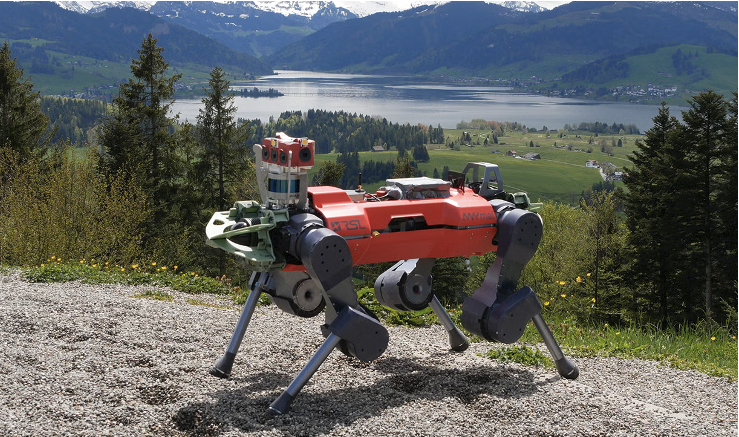
\includegraphics[width=0.47\textwidth]{pics/Introduction/Legged_Robot_high_resolution.pdf}
        \label{fig:introduction_applications_legged}
    }
    \hfill
    \subfigure[Industrial robot]{
        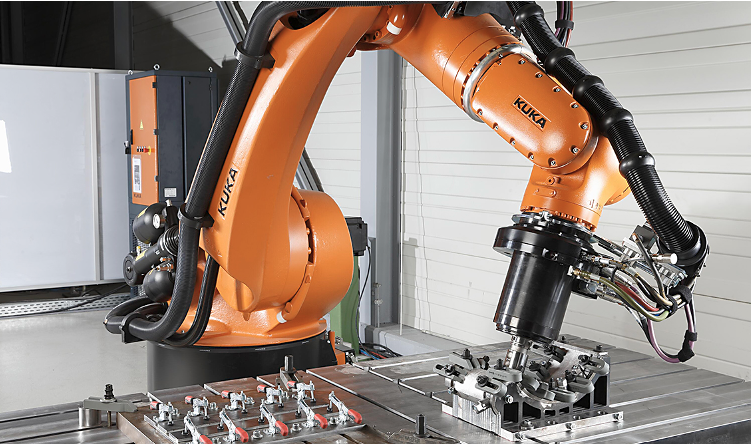
\includegraphics[width=0.47\textwidth]{pics/Introduction/KUKA_high_resolution.pdf}
        \label{fig:introduction_applications_kuka}
    }
    \caption{Examples of robotic systems composed of coupled rigid bodies: (a) legged
    locomotion taken from \cite{Intro_Legged} and (b) industrial manipulation taken from \cite{Intro_KUKA}.}
    \label{fig:introduction_applications}
\end{figure}

In addition to a large number of system variables, rigid-body attitudes
belong to rotation groups, considered as Lie groups, rather than to a Euclidean vector
space. Joint constraints couple the configuration of neighbouring bodies, and the
equations of motion couple states and controls over time \cite{Sangli2025}. Consequently, even a
finite-horizon problem without contact or obstacles generally contains nonlinear
equalities and nonconvex rotation constraints. Its feasible set can have several
disconnected regions, and its objective can contain many local minima \cite{Kang_2026Fast}.
Moreover, the continuous-time dynamics are high dimensional as state and control trajectories
are functions of time. So any numerical
solution must discretize these problems. Nevertheless, classic global optimization methods simplify
the dynamics of robotic systems by approximating them with simpler models \cite{Sangli2025}. 
Thereby, the discrete dynamics can differ from the continuous dynamics through 
loss of geometric structure and manifold drift, 
which results in deviations from the true solution and 
numerical infeasibility \cite{Marsden2001}.

Currently, nonlinear programming is one of the most common approaches for computing robot 
trajectories. Starting from an initial guess, these methods repeatedly adjust the states and 
control inputs to find a trajectory with a low objective value that satisfies the given 
constraints \cite{Betts1998TrajectoryOptimization,tedrake_underactuated}. Sequential convex 
methods, such as TrajOpt, follow a similar idea but replace the original difficult problem 
with a sequence of simpler convex problems \cite{Schulman2014TrajOpt}. Both approaches can 
find useful motions efficiently, even for relatively large robot models. However, the final 
result may depend strongly on the initial guess and is generally only locally optimal.
Sampling-based methods instead explore many possible configurations and connect them to 
construct a path. Although some of these methods are asymptotically optimal, a path obtained 
after a finite computation does not provide a certificate of global optimality 
\cite{KaramanFrazzoli2011Sampling}.

To address the limitations of local methods, this thesis investigates semidefinite 
programming (SDP) for multibody systems. An SDP is a convex optimization problem formulated
using matrix variables. Instead of solving the original nonconvex motion-planning problem directly, a semidefinite 
relaxation constructs a convex approximation that can be solved reliably and provides a lower 
bound on the globally optimal objective value \cite{VandenbergheBoyd1996SDP,Lasserre2001Global}. 
In contrast, a feasible trajectory, for example generated by a local optimization method
such as NLP or TrajOpt, provides an upper bound. 
If the suboptimality gap between the SDP lower bound and the feasible-trajectory 
upper bound is within the specified numerical tolerance, the trajectory is \emph{certified} 
as globally optimal for the considered discrete motion-planning problem \cite{Sangli2025}.

However, realistic trajectory optimization also requires a discrete model that represents
the rigid-body dynamics accurately. Lie group variational integrators (LGVIs) discretize the 
equations of motion directly on the configuration manifold and update rotations through the 
Lie-group structure \cite{Marsden2001,Lee2008}. Consequently, the numerical rotations remain 
on the rotation group. LGVIs also preserve important 
geometric properties of the mechanical system, such as its symplectic structure and 
energy conservation over a long time duration \cite{Sangli2025}. 

Therefore, the key idea of this thesis is to combine these two approaches. For the considered 
rigid-body systems, the LGVI dynamics can be expressed through low-degree polynomial equations. 
The resulting polynomial motion-planning problem can then be approximated by a Moment--SOS 
semidefinite relaxation \cite{Sangli2025}. Thereby, the LGVI provides a structure-preserving 
model of the rigid-body dynamics, while the SDP provides a global lower bound and 
certifies global optimality.
This is the case when the relaxation is tight and a feasible trajectory can be extracted. 
The complete 
concept is summarized in Figure~\ref{fig:intro_pipeline}.

\begin{figure}[t!]
    \centering

    \begin{tikzpicture}[
        >=Latex,
        node distance=5mm,
        block/.style={
            rounded corners=1.5mm,
            draw=black!45,
            fill=black!2,
            thick,
            align=center,
            text width=8.8cm,
            minimum height=0.75cm,
            font=\small
        },
        titled/.style={
            rectangle split,
            rectangle split parts=2,
            rectangle split part align={left,center},
            rounded corners=2mm,
            line width=1pt,
            text width=9cm,
            inner xsep=2mm,
            inner ysep=1mm,
            font=\small
        },
        arrow/.style={
            -{Latex[length=2.2mm]},
            thick,
            draw=black!65
        }
    ]

    % Main problem
    \node[
        titled,
        draw=tum_blue,
        rectangle split part fill={
            tum_blue,
            tum_blue!8!white
        }
    ] (problem)
    {
        \textcolor{white}{\figureboxtitle{Main Problem}}
        \nodepart{second}
        Nonlinear and nonconvex rigid-body trajectory optimization
    };

    \node[
        block,
        below=7mm of problem
    ] (lgvi)
    {
        Lie group variational discretization\\[-1mm]
        \scriptsize structure-preserving rigid-body dynamics
    };

    \node[
        block,
        below=of lgvi
    ] (pop)
    {
        Polynomial motion-planning formulation
    };

    \node[
        block,
        below=of pop
    ] (sdp)
    {
        Sparse Moment--SOS semidefinite relaxation\\[-1mm]
        \scriptsize convex global lower bound
    };

    % Key idea
    \node[
        titled,
        draw=tum_orange,
        rectangle split part fill={
            tum_orange,
            orange!8!white
        },
        below=7mm of sdp
    ] (idea)
    {
        \textcolor{white}{\figureboxtitle{Key Idea}}
        \nodepart{second}
        Structure-preserving LGVI dynamics combined with
        semidefinite relaxation
    };

    \draw[arrow] (problem) -- (lgvi);
    \draw[arrow] (lgvi) -- (pop);
    \draw[arrow] (pop) -- (sdp);
    \draw[arrow] (sdp) -- (idea);

    \end{tikzpicture}

    \caption{Framework of this thesis.
    Lie group variational discretization provides structure-preserving
    rigid-body dynamics, while sparse semidefinite relaxation provides
    a convex lower bound for the resulting polynomial motion-planning
    problem.}
    \label{fig:intro_pipeline}
\end{figure}

This thesis investigates a 3D pendulum as a 
single-rigid-body system and an Acrobot as a constrained and underactuated multibody system. 
The main contributions of this thesis are:

\begin{itemize}
\item The explanation of an LGVI for the controlled and unforced 3D pendulum on $\mathrm{SO}(3)$, 
providing a structure-preserving discrete model of a single rigid body.

\item The derivation of a constrained LGVI for the Acrobot in maximal coordinates on 
$(\mathrm{SO}(2)\times \mathbb{R}^2)^2$.
Thereby, the positions and rotations of both rigid links are represented separately 
and connected through holonomic joint constraints.

\item The numerical implementation and validation of both LGVI models, including the 
preservation of the rotation and joint constraints, and the conserved long-term energy 
behavior.

\item The formulation of the 3D-pendulum polynomial optimization problem (POP) as a polynomial 
optimization problem and its solution through a sparse Moment-SOS semidefinite relaxation. 
This is followed by an assessment of relaxation tightness, extraction feasibility, and the availability 
of global-optimality certificates.

\item The formulation of the Acrobot POP using a reduced polynomial 
model, problem-specific sparse SDP structures and its solution through 
a sparse Moment-SOS semidefinite relaxation.
Finally, the evaluation of the extracted trajectories and their global optimality certificates.
Thereby, the evaluation is extended to a closed-loop implementation.
\end{itemize}

\section{Problem Statement}
\label{sec:introduction_problem_statement}

The framework illustrated in Figure \ref{fig:intro_pipeline} addresses the
following general motion planning problem. Thereby, the objective is to optimize the path 
of a rigid-body system from
an initial configuration towards a desired configuration, while respecting the system's
dynamics, geometric structure, joint connections, and physical limits.
The motion is considered over a finite horizon divided into $N$ intervals. Let $\bm{Y}_k$ describe
the configuration and discrete motion of the system at step $k$, let $\bm{U}_k$ denote
the applied control input, and let $\bm{\lambda}_k$ contain joint-constraint multipliers
when several bodies are connected. The rigid links are indexed by
$i\in\mathcal B:=\{1,\ldots,n_{\mathrm b}\}$. At a high level, the corresponding
motion-planning problem can be written as
\begin{subequations}
\label{eq:problem_statement}
\begin{align}
p^\star =
\min_{\{\bm{Y}_k\}_{k=0}^{N},\{\bm{U}_k,\bm{\lambda}_k\}_{k=1}^{N}}
\quad & \Psi(\bm{Y}_N)+\sum_{k=0}^{N-1}\psi(\bm{Y}_k,\bm{U}_{k+1},\bm{\lambda}_{k+1}),
\label{eq:problem_statement_objective}\\
\text{s.t.}\quad
&\bm{Y}_0=\bm{Y}_{\mathrm{init}},
\label{eq:problem_statement_initial}\\
&\mathcal D_i(\bm{Y}_{k+1},\bm{Y}_k,\bm{U}_{k+1},\bm{\lambda}_{k+1})=0,
\label{eq:problem_statement_dynamics}\\
&(\bm{Y}_{k+1}, \bm{Y}_k,\bm{U}_{k+1},\bm{\lambda}_{k+1})\in\mathcal{A}_k,
\label{eq:problem_statement_admissible}
\end{align}
\end{subequations}

for $k=0,\ldots,N-1$. The objective combines the terminal cost $\Psi$ with the running cost $\psi$. Additionally, the
constraints $\mathcal D_i=0$ represent the discrete rigid-body dynamics of link $i$.
For this compact statement, the admissible set $\mathcal A_k$ collects the Lie-group constraints,
inequality constraints, and control bounds that are written separately as
$\mathcal Y_i$, $\mathcal H$, and $\bm{U}_{\min}\leq \bm{U}_{k+1}\leq \bm{U}_{\max}$ in
Chapter~\ref{chapter:certifiable_trajectory_optimization}. Therefore, \eqref{eq:problem_statement}
summarizes the physical requirements of the problem, generalizing it to any robotic system \cite{Kang_2026Fast}. 

Generally, the objective appears simple. However, for many robotic systems composed of many rigid bodies, 
the equality constraints $\mathcal D_i$ are nonlinear, and
the rotation constraints and equations of
motion make the feasible set nonconvex. The LGVI formulation is useful because the
considered dynamics can be expressed by low-degree
polynomials and have energy-conservation properties \cite{Sangli2025}. 
After collecting all scalar decision variables in
$\bm{z}\in\mathbb{R}^{n_z}$, \eqref{eq:problem_statement} takes the standard
polynomial form
\begin{equation}
\label{eq:problem_statement_polynomial_form}
p^\star=\min_{\bm{z}\in\mathbb{R}^{n_z}}p(\bm{z})
\quad\text{s.t.}\quad
h_i(\bm{z})=0,\ i\in\mathcal{E},
\qquad
g_j(\bm{z})\geq0,\ j\in\mathcal{J},
\end{equation}
\cite{Yang2024Semidefinite}. Here, $p^*$ is the globally optimal value, $h_i$ are polynomial equality constraints,
and $g_j$ are polynomial inequality constraints, with their respective sets $\mathcal{E}$ and $\mathcal{J}$.
This polynomial optimization problem remains nonconvex. At a selected relaxation
order $\kappa$, a Moment-SOS semidefinite relaxation replaces \eqref{eq:problem_statement_polynomial_form}
by a convex problem and returns a global lower bound $\gamma_\kappa^\star$. In contrast, every
verified feasible trajectory $\hat{\bm{z}}$ provides an upper bound through its objective
value. Therefore, the globally optimal value $p^\star$ of the objective is bounded by
\begin{equation}
\label{eq:problem_statement_bounds}
\gamma_\kappa^\star\leq p^\star\leq p(\hat{\bm{z}}).
\end{equation}
If the lower and upper bounds agree within specified numerical tolerances, the
feasible trajectory is certified as globally optimal \cite{Lasserre2001Global}.

Therefore, the central research question of this thesis is as follows:

\begin{quote}
\emph{What are the capabilities and limitations of combining structure-preserving Lie group variational 
integrators with semidefinite relaxation to obtain feasible and certifiably 
optimal trajectories for single- and multi rigid-body systems?}
\end{quote}

This question is investigated by first deriving structure-preserving LGVI models,
then formulating the resulting discrete dynamics as polynomial optimization
problems, and finally evaluating the SDP relaxations in terms of feasibility,
tightness, certifiability, and computational cost.

\section{Related Work}
\label{sec:introduction_related_work}

\paragraph{Trajectory optimization and global planning}

Trajectory optimization represents a robot motion by a finite sequence of states
and control inputs. Direct nonlinear programming methods are widely used
because they can solve large problems efficiently, described in
\cite{Betts1998TrajectoryOptimization,tedrake_underactuated}. Sequential convex
methods such as TrajOpt, from \cite{Schulman2014TrajOpt}, similarly replace the original problem by a sequence of
simpler subproblems. These approaches can produce useful
motions fast, but generally converge only to a local solution and therefore
depend on the initial guess. Sampling-based planners such as PRM$^*$ and RRT$^*$
offer asymptotic optimality, but not a global certificate after a finite computation
\cite{KaramanFrazzoli2011Sampling}. Mixed-integer formulations of 
\cite{DeitsTedrake2014Footstep,DaiIzattTedrake2019IK} provide global
statements for selected problems such as footstep placement and inverse kinematics,
although their computational cost and model approximations are inefficient for
general multibody dynamics.
\cite{Posa2014Contact,Manchester2019ContactVI}.
investigated contact-implicit methods
by including contact forces and mode changes directly in the optimization.

\paragraph{Geometric mechanics and variational integration}

Rigid-body attitudes naturally belong to Lie groups rather than Euclidean vector
spaces. The required foundations of Lie groups, mechanical symmetry, rigid-body
mechanics, inertia, and matrix analysis are provided in
\cite{Hall2000LieGroups,MarsdenRatiu1999,Benacquista2018ClassicalMechanics,
RITInertiaTable216,GallierQuaintance2020LinearAlgebra,YanaiTakeuchiTakane2011SVD}.
Classical integration methods are summarized by Butcher
\cite{butcher2016numerical}, whereas geometric integration emphasizes the
preservation of mechanical structure over long simulations
\cite{Hairer1994,Leimkuhler_Reich_2005}. Projection can restore manifold
constraints after a numerical step \cite{Hairer2000}, while Lie-group integrators
update the configuration directly on the group \cite{CELLEDONI2003421}.
Retraction maps such as the Cayley transform provide a
computational implementation of the implicit Lie-group update, described in
\cite{Arieh_Cayley_Motivation,ColomboJimenez2012SO3_Cayley,
Barbero-Linan2023_Cayley_Formula}.

Variational integrators derive the discrete equations of motion from a discrete
action principle and thereby preserve important geometric properties of the
continuous mechanics, which are defined in \cite{Marsden2001}. 
\cite{Lee2008} develops this approach directly on
matrix Lie groups and applies it to rigid-body mechanics, optimal control, and the
full-body problem. The approach is extended in
\cite{Lee2007,LeeLeokMcClamroch2007DiscreteControlSystems}. The 3D pendulum
provides a compact benchmark for these rotational dynamics \cite{Shen20043DPendulum}.
For multibody systems, maximal coordinates assign a pose to every body and impose
joints through algebraic constraints, defined in 
\cite{BrudigamManchester2021VariationalIntegrators,BrudigamManchester2021LQR}.
These works form the basis for the 3D-pendulum and maximal-coordinate Acrobot LGVIs
derived in this thesis.

\paragraph{Polynomial optimization and sparse semidefinite relaxation}

Semidefinite programming is a convex optimization framework
\cite{VandenbergheBoyd1996SDP}. Moment-SOS methods use it to relax polynomial
optimization problems and obtain global lower bounds. 
\cite{Putinar1993Positive,Lasserre2001Global,Yang2024Semidefinite} establish their 
theoretical basis is
given by positivity certificates and the Lasserre hierarchy. However,
tightness at a selected relaxation order is not guaranteed, as discussed in
\cite{Nie2014FiniteConvergence}. Dense moment matrices grow rapidly with the number
of variables. Correlative sparsity instead constructs smaller overlapping matrices
and can preserve convergence under suitable conditions given in
\cite{Waki2006Sparse,Lasserre2006Sparse}.

\cite{Sangli2025} combine Lie-group variational integrators with sparse moment relaxation
for multibody motion planning and therefore provide the closest methodological
foundation for this thesis. \cite{Kang_2026Fast} show that specialized
sparse formulations and first-order GPU solvers can substantially accelerate
certifiable trajectory optimization. \cite{Kang_2025Global} extend sparsity-rich
relaxations to contact-rich planning. These developments
demonstrate the potential of the approach, while also showing that relaxation size
and solver choice remain decisive. This thesis uses the interior-point solver MOSEK
for optimization \cite{MOSEK}.
Related SDP-based MPC research further illustrates the relevance of repeatedly
solving relaxations in closed loop, as shown in \cite{Hartmann_2026SDP}. The implementation and
experiments presented in this thesis are documented in the open-source
repository \cite{Elshani2026CTO_GitHub}.

\section{Research Gap}
\label{sec:introduction_research_gap}

The connection between LGVIs and semidefinite relaxation has already
been investigated in recent works. However, it does not provide certifiably optimal trajectories for every
problem. \cite{Sangli2025} combines LGVIs with sparse Moment-SOS relaxations for
single- and multibody systems. Still, some relaxations are not
tight, requiring the extracted solutions to be refined using nonlinear programming (NLP),
in order to obtain feasible trajectories.
Similarly, \cite{Kang_2026Fast,Kang_2025Global} develop faster solvers and robotics-specific sparse
formulations, but the reported suboptimality
gaps remain problem-dependent and range from below $(1\%)$ to more than
$(30\%)$ for some problems. Therefore, semidefinite relaxation can provide useful lower bounds and
trajectory candidates, but does not generally guarantee a feasible or certifiably
optimal trajectory.

Accordingly, a remaining question is how reliably the complete LGVI-SDP framework can be applied to systems of 
increasing dynamical complexity.
In particular,
relaxation tightness and feasible trajectory extraction are problem-dependent, and
become more difficult for constrained and underactuated multibody systems. 
This thesis addresses this gap by comparing the complete
pipeline on a single-body benchmark and a constrained underactuated multibody
system. It further investigates whether repeated first-control extraction can
generate feasible closed-loop trajectories when the complete open-loop relaxation
is not tight.

The contribution of this thesis is an empirical assessment showing that SDP can generate feasible trajectories 
using a closed-loop setup and certifiably optimal trajectories in an open-loop setting
for tight relaxations, for rigid-body problems of increasing 
difficulty. Additionally, the offline SDP-MPC implementation can generate feasible stabilizing 
trajectories for harder problems, which can serve as reference or training data for 
controllers and learning-based methods, such as imitation learning or offline reinforcement 
learning.

\section{Thesis Structure}
\label{sec:introduction_structure}

Following the introduction, Chapter \ref{chapter:preliminaries_lie_groups} 
introduces the required matrix Lie groups and Lie algebras. 

Secondly, Chapter \ref{chapter:continous_mechanics_of_rigid_bodies_on_lie_groups} 
develops continuous Lagrangian mechanics on Lie groups,
and derives the continuous 3D-pendulum model, which momentum conservation
property is verified.

Chapter \ref{chapter:discrete_mechanics_for_rigid_bodies_on_lie_groups}
introduces discrete mechanics and LGVIs, first for a single rigid body
and subsequently for constrained multibody systems using maximal coordinates.
Thereby, the LGVI dynamics of a 3D pendulum and a two-link Acrobot are derived. 

Therefore, Chapter \ref{chapter:certifiable_trajectory_optimization}
formulates their trajectory-optimization problems,
introduces semidefinite and Moment--SOS relaxations, defines sparse clique
constructions and certification diagnostics, and presents a closed-loop
SDP implementation for the Acrobot.

Consequently, the numerical simulation  and optimization results 
of the 3D-pendulum and Acrobot are 
evaluated in Chapter \ref{chapter:evaluation}.

Chapter \ref{chap:discussion} discusses the previous results, especially 
the non-certifiable cases and the remaining computational and modeling limitations. 

Finally, Chapter \ref{chap:conclusion} summarizes the
findings and gives the final outlook, proposing future research directions.

%\input{./chapters/MainPart.tex}
\chapter{Preliminaries on Special Embedded Matrix Lie Groups}
\label{chapter:preliminaries_lie_groups}

This chapter summarizes the Lie group notation required for the continuous 
and discrete rigid-body mechanics developed in Chapters \ref{chapter:continous_mechanics_of_rigid_bodies_on_lie_groups} and \ref{chapter:discrete_mechanics_for_rigid_bodies_on_lie_groups}, following the definitions of Lie groups and Lie algebras in \cite{Hall2000LieGroups} and the geometric-mechanics notation in \cite{Lee2008}.

\section{Special Matrix Lie Groups}
\label{sec:special_matrix_lie_groups}

A Lie group is a smooth manifold that is also a group, where multiplication and inversion are smooth maps. A real matrix Lie group is a closed subgroup
$G\subset\mathrm{GL}(n,\mathbb{R})$. Its group operation is matrix
multiplication, and it is an embedded smooth manifold for which
multiplication and inversion are smooth maps
\cite{Hall2000LieGroups}.

Rotations in \(n\) dimensions are represented by the special orthogonal group
\begin{equation}
    \mathrm{SO}(n)
    =
    \left\{
        \bm{R}\in\mathbb{R}^{n\times n}
        \;\middle|\;
        \bm{R}^{\top}\bm{R}=\bm{I}_{n},\;
        \det(\bm{R})=1
    \right\}.
    \label{eq:so_group}
\end{equation}
The groups \(\mathrm{SO}(2)\) and \(\mathrm{SO}(3)\) describe planar and spatial rotations \cite{Lee2008}.

Combined rotational and translational motion is represented by the special Euclidean group
\begin{equation}
    \mathrm{SE}(n)
    =
    \left\{
        \bm{T}
        =
        \begin{bmatrix}
            \bm{R} & \bm{p}\\
            \bm{0} & 1
        \end{bmatrix}
        \;\middle|\;
        \bm{R}\in\mathrm{SO}(n),\;
        \bm{p}\in\mathbb{R}^{n}
    \right\}.
    \label{eq:se_group}
\end{equation}
Here, \(\bm{R}\) denotes the attitude and \(\bm{p}\) the position \cite{Hall2000LieGroups}. However, in this thesis 
rotations and translations are represented separately
in maximal coordinates, elaborated in Section \ref{sec:multi_body_systems}. Therefore, the derivations mainly use
$\mathrm{SO}(n)$ and its Lie algebra $\mathrm{so}(n)$.

\section{Special Lie Algebras}
\label{sec:special_lie_algebras}

\paragraph{Lie algebras and the exponential map}
\cite{Hall2000LieGroups} defines the Lie algebra \(\mathfrak{g}\) of a matrix Lie group \(G\) as its tangent space at the identity,
\begin{equation}
    \mathfrak{g}=T_{e}G.
    \label{eq:lie_algebra_tangent_space}
\end{equation}
For matrix Lie groups, the Lie bracket $[\cdot,\cdot]: \mathfrak{g} \times \mathfrak{g} \to \mathfrak{g}$ 
is defined as
\begin{equation}
    [\bm{a},\bm{b}]
    =
    \bm{a}\bm{b}-\bm{b}\bm{a},
    \qquad
    \bm{a},\bm{b}\in\mathfrak{g},
    \label{eq:matrix_lie_bracket}
\end{equation}
which is bilinear and skew-symmetric \cite{Hall2000LieGroups}. The Lie algebras corresponding to \(\mathrm{SO}(n)\) and \(\mathrm{SE}(n)\) are
\begin{align}
    \mathfrak{so}(n)
    &=
    \left\{
        \bm{\omega}\in\mathbb{R}^{n\times n}
        \;\middle|\;
        \bm{\omega}^{\top}=-\bm{\omega}
    \right\}
    \label{eq:so_algebra},
    \qquad
    &\mathfrak{so}(n) = T_{e}\mathrm{SO}(n)
    \\
    \mathfrak{se}(n)
    &=
    \left\{
        \begin{bmatrix}
            \bm{\omega} & \bm{v}\\
            \bm{0}^{\top} & 0
        \end{bmatrix}
        \;\middle|\;
        \bm{\omega}\in\mathfrak{so}(n),\;
        \bm{v}\in\mathbb{R}^{n}
    \right\},
    \qquad
    &\mathfrak{se}(n) = T_{e}\mathrm{SE}(n).
    \label{eq:se_algebra}
\end{align}
For \(\mathrm{SO}(2)\), \cite{Lee2008} defines the hat map $(\cdot)^\wedge: \mathbb{R} \rightarrow \mathfrak{so}(2)$ as
\begin{equation}
    \widehat{\omega}
    =
    \begin{bmatrix}
        0 & -\omega\\
        \omega & 0
    \end{bmatrix},
    \label{eq:hat_map_so2}
\end{equation}
with $\omega \in \mathbb{R}$.
Additionally, for \(\mathrm{SO}(3)\), the hat map \((\cdot)^{\wedge}:\mathbb{R}^{3}\rightarrow\mathfrak{so}(3)\) is defined by
\begin{equation}
    \widehat{\bm{\omega}}
    =
    \begin{bmatrix}
        0 & -\omega_{3} & \omega_{2}\\
        \omega_{3} & 0 & -\omega_{1}\\
        -\omega_{2} & \omega_{1} & 0
    \end{bmatrix},
    \qquad
    \widehat{\bm{\omega}}\bm{b}=\bm{\omega}\times\bm{b},
    \label{eq:hat_map_so3}
\end{equation}
with $\bm{\omega}, \bm{b} \in \mathbb{R}^3$ and the corresponding inverse map \((\cdot)^{\vee}: \mathfrak{so}(3) \rightarrow \mathbb{R}^3\).

The matrix exponential of an $n\times n$ matrix $\bm{X}$
\begin{equation}
    \exp(\bm{X})=\sum_{m=0}^{\infty} \frac{\bm{X}^m}{m!}
    \label{eq:matrix_exponential}
\end{equation}
defines the exponential map \(\exp:\mathfrak{g}\rightarrow G\) as a local diffeomorphism between a neighborhood of \(\bm{0}\in\mathfrak{g}\) and a neighborhood of \(e\in G\) \cite{Hall2000LieGroups,Lee2008}.

\paragraph{Left and right translations}
For \(\bm{g},\bm{h}\in G\), the left and right translation maps are
\begin{equation}
    \mathbb{L}_{\bm{h}}(\bm{g})=\bm{h}\bm{g},
    \qquad
    R_{\bm{h}}(\bm{g})=\bm{g}\bm{h}.
    \label{eq:left_right_translation}
\end{equation}
Thereby, \cite{Lee2008} states that for a differentiable matrix-valued curve $\bm{g}(t) \in G$, the left-trivialized or body-fixed velocity $\bm{\xi} \in \mathfrak{g}$ is given by
\begin{equation}
    \bm{\xi}=\bm{g}^{-1}\dot{\bm{g}},
    \qquad
    \dot{\bm{g}}=\bm{g}\bm{\xi}.
    \label{eq:left_trivialized_velocity}
\end{equation}

\begin{proposition}[Differential of left translation on a matrix Lie group: $T_{\bm{x}}\mathbb{L}_{\bm{h}}$]
Let $G\subset GL(n,\mathbb{R})$ be a matrix Lie group.
For $\bm{h}\in G$, define $\mathbb{L}_{\bm{h}}:G\to G$ by $\mathbb{L}_{\bm{h}}(\bm{g})=\bm{h}\bm{g}$ \cite{Hall2000LieGroups}.
Then for each $\bm{x}\in G$ the differential
\[
T_{\bm{x}}\mathbb{L}_{\bm{h}}: T_{\bm{x}}G \to T_{\bm{h}\bm{x}}G,
\]
of the left translation map $\mathbb{L}_{\bm{h}}:G\to G$ is given by
\begin{align}\label{eq:preliminaries_differential_left_translation}
T_{\bm{x}}\mathbb{L}_{\bm{h}}(\bm{v})=\bm{h}\bm{v}.
\end{align}
\end{proposition}
\begin{proof}
By the definition of the tangent space of an embedded submanifold given in \cite{Hall2000LieGroups}, there exists a smooth matrix-valued curve $\bm{\gamma}: (-\epsilon,\epsilon) \to G$ with $\bm{\gamma}(0)=\bm{x}$ and the tangent matrix $\dot{\bm{\gamma}}(0)=\bm{v} \in T_{\bm{x}}G$.
In \cite{Lee2008}, the differential is defined as
\[
T_{\bm{x}}\mathbb{L}_{\bm{h}}(\bm{v})=\left.\frac{d}{dt}\mathbb{L}_{\bm{h}}(\bm{\gamma}(t))\right|_{t=0}
=\left.\frac{d}{dt}(\bm{h}\bm{\gamma}(t))\right|_{t=0}=\bm{h}\dot{\bm{\gamma}}(0),
\]
with the left translation map $\mathbb{L}_{\bm{h}}(\bm{g})=\bm{h}\bm{g}$. Since $\bm{h}$ is constant and $\dot{\bm{\gamma}}(0)=\bm{v}$, it follows that
\[
T_{\bm{x}}\mathbb{L}_{\bm{h}}(\bm{v})=\bm{h}\dot{\bm{\gamma}}(0)=\bm{h}\bm{v}.
\]
\end{proof}

It can be observed that $\mathbb{L}_{\bm{h}}(\bm{g})=\bm{h}\bm{g}$ and $T_{\bm{x}}\mathbb{L}_{\bm{h}}(\bm{v})=\bm{h}\bm{v}$ have the same matrix expression, but act on different objects. The left translation map $\mathbb{L}_{\bm{h}}(\bm{g})$ multiplies group elements $\bm{g} \in G$, while its differential is the pushforward of tangent matrices $\bm{v} \in T_{\bm{x}}G \subset \mathbb{R}^{n \times n}$. The differential of a left translation can be applied to the special embedded matrix Lie groups $SO(n)$ and their corresponding Lie algebras $\mathfrak{so}(n)$. 

\paragraph{Differential of left translation $T_{\bm{R}}\mathbb{L}_{\bm{H}}$ on $SO(n)$}

The left translation map in $SO(n)$ is defined as $\mathbb{L}_{\bm{H}}(\bm{R}) = \bm{H}\bm{R}$ with $\bm{H},\bm{R} \in G$. Applied to eq. \eqref{eq:preliminaries_differential_left_translation} with $\bm{v} \in T_{\bm{R}}G$, it follows that
\begin{align*}
    T_{\bm{R}}\mathbb{L}_{\bm{H}}(\bm{v})= \bm{H}\bm{v}.
\end{align*}
The tangent matrix $\bm{v} \in T_{\bm{R}}G$ can be represented by $\bm{v} = T_{e}\mathbb{L}_{\bm{R}}(\bm{\omega}) = \bm{R}\bm{\omega}$ using the left translation map of $\bm{\omega} \in \mathfrak g := \mathfrak{so}(n)$, resulting in
\begin{align}\label{eq:preliminaries_differential_left_SO}
    T_{\bm{R}}\mathbb{L}_{\bm{H}}(\bm{R}\bm{\omega}) = \bm{H}(\bm{R}\bm{\omega}).
\end{align}

%\paragraph{Differential of left translation $T_g\mathbb{L}_h$ on $SE(n)$}

%The left translation map in $SE(n)$ is defined as $\mathbb{L}_{h}(g) = hg$ with $h,g \in G$. Applied to eq. \eqref{eq:preliminaries_differential_left_translation} with $v \in T_{g}G$, it follows that
%\begin{align*}
%    T_{g}\mathbb{L}_{h}(v)= hv.
%\end{align*}
%The tangent vector $v \in T_gG$ can be represented by $v = T_{e}\mathbb{L}_{g}(\xi) = g\xi$ using the left translation map of $\xi \in \mathfrak g := \mathfrak{se}(n)$ resulting in
%\begin{align}\label{eq:preliminaries_differential_left_SE}
%    T_g\mathbb{L}_h(g \xi) = h(g \xi).
%\end{align}



\paragraph{Adjoint and coadjoint operators}
\cite{Lee2008} introduces the adjoint operator $\operatorname{Ad}_{\bm{g}}: \mathfrak{g} \to \mathfrak{g}$ as
\begin{equation}
    \operatorname{Ad}_{\bm{g}}\bm{\eta}
    =
    \bm{g}\bm{\eta}\bm{g}^{-1}.
    \label{eq:adjoint_matrix}
\end{equation}
Its derivative  $\operatorname{ad}_{\bm{\xi}}: \mathfrak{g} \to \mathfrak{g}$ is defined as
\begin{equation}
    \operatorname{ad}_{\bm{\xi}}\bm{\eta}
    =
    \left.\frac{\mathrm{d}}{\mathrm{d}\epsilon}\right|_{\epsilon=0}
    \operatorname{Ad}_{\exp(\epsilon\bm{\xi})}\bm{\eta}
    =
    [\bm{\xi},\bm{\eta}]
    = \bm{\xi}\bm{\eta} - \bm{\eta}\bm{\xi},
    \label{eq:ad_lie_bracket}
\end{equation}
using the Lie bracket $[\cdot,\cdot]$ defined in \eqref{eq:matrix_lie_bracket}.

Let \(\mathfrak{g}^{*}\) be the dual space of \(\mathfrak{g}\). The notation $\langle\bm{\mu},\bm{\xi}\rangle = \bm{\mu}(\bm{\xi})$ denotes the pairing of a covector \(\bm{\mu}\in\mathfrak{g}^{*}\) with a vector \(\bm{\xi}\in\mathfrak{g}\) \cite{Lee2008}. 
Using the pairing, the coadjoint operator \(\operatorname{Ad}_{\bm{g}}^{*}:\mathfrak{g}^{*}\rightarrow\mathfrak{g}^{*}\) is defined as 
\begin{equation}
    \left\langle
        \operatorname{Ad}_{\bm{g}}^{*}\bm{\mu},
        \bm{\xi}
    \right\rangle
    =
    \left\langle
        \bm{\mu},
        \operatorname{Ad}_{\bm{g}}\bm{\xi}
    \right\rangle.
    \label{eq:coadjoint_definition}
\end{equation}
Its derivative \(\operatorname{ad}_{\bm{\eta}}^{*}:\mathfrak{g}^{*}\rightarrow\mathfrak{g}^{*}\) is given by
\begin{align}
    \left\langle\operatorname{ad}_{\bm{\eta}}^{*}\bm{\mu},\bm{\xi}\right\rangle
    &=
    \left\langle\bm{\mu},\operatorname{ad}_{\bm{\eta}}\bm{\xi}\right\rangle
    =
    \left\langle\bm{\mu},[\bm{\eta},\bm{\xi}]\right\rangle
    =
        \left\langle\bm{\mu},\bm{\eta}\bm{\xi} - \bm{\xi}\bm{\eta}\right\rangle
.
    \label{eq:coad_definition}
\end{align}

Additionally, the pairing can be used to define the inner product on the dual space of the Lie algebra \cite{Lee2008}. Using the trace inner product, $\mathfrak{so}(n)$ is identified with its
dual. For $n\in\{2,3\}$, the hat map gives
\begin{equation}
    \left\langle\widehat{\bm a},\widehat{\bm b}\right\rangle
    =
    \frac{1}{2}\operatorname{tr}\!\left(
        \widehat{\bm a}^{\top}\widehat{\bm b}
    \right)
    =
    \bm a^{\top}\bm b = \bm{a} \cdot \bm{b},
    \label{eq:trace_inner_product}
\end{equation}
where $\bm a,\bm b\in\mathbb{R}$ for $n=2$ and
$\bm a,\bm b\in\mathbb{R}^{3}$ for $n=3$.


\paragraph{Variations on Matrix Lie Groups}

For $g\in G$ and $\eta\in\mathfrak{g}=T_eG$, define the local variation
curve $\gamma:(-c,c)\rightarrow G$ by
\begin{equation}
    \gamma(\epsilon)
    =
    g\exp(\epsilon\eta),
    \qquad c>0,
    \label{eq:variation_curve_matrix_lie_group}
\end{equation}
where $\epsilon$ is the variation parameter. Since
$\exp(\epsilon\eta)\in G$, the curve $\gamma(\epsilon)$ remains in
$G$ and satisfies $\gamma(0)=g$ \cite{Lee2008}. The corresponding
infinitesimal variation is
\begin{equation}
    \delta g
    =
    \left.
    \frac{d}{d\epsilon}
    \right|_{\epsilon=0}
    \gamma(\epsilon)
    =
    \left.
    \frac{d}{d\epsilon}
    \right|_{\epsilon=0}
    g\exp(\epsilon\eta)
    =
    g\eta
    =
    T_e\mathbb{L}_g(\eta)
    \in T_gG.
    \label{eq:infinitesimal_variation_matrix_lie_group}
\end{equation}


%Explain brackets
%Inner product 
%-> Pairs

\chapter{Continuous Mechanics of Rigid Bodies on Lie Groups}
\label{chapter:continous_mechanics_of_rigid_bodies_on_lie_groups}


This chapter introduces the continuous mechanics of rigid bodies on Lie groups, which is the foundation for the discrete mechanics formulation in Chapter~\ref{chapter:discrete_mechanics_for_rigid_bodies_on_lie_groups}. 
Therefore, Section \ref{sec:continuous_lagrangian_mechanics} presents the representation of geometric mechanics on Lie groups
by deriving the Euler-Lagrange equations and the Legendre transformation. Moreover, the properties of the Lagrangian flow are discussed. Consequently, 
Section \ref{section:continuous_3D_pendulum} applies the derived framework to the unforced 3D-pendulum as an example of a mechanical system on a Lie group, and verifies the momentum preservation properties of the Lagrangian 
flow of the model, based on the work of \cite{Lee2008}. 

% Chapter 3.1: Lagrangian Mechanics
% Required cross-reference in Chapter 2:
% Add \label{prop:infinitesimal_variation_matrix_lie_group}
% immediately after
% \begin{proposition}[Infinitesimal variation on a matrix Lie group]

\section{Lagrangian Mechanics}
\label{sec:continuous_lagrangian_mechanics}

Differential geometry provides a framework for describing geometric mechanics, by
exploring the geometric structure of a Lagrangian or Hamiltonian system \cite{Lee2008}.
Thereby, Lagrangian mechanics describes the motion of a mechanical system through
a variational principle. Instead of directly discretizing or integrating
the equations of motion, the trajectory is obtained from the stationary
value of the action integral. This formulation provides the continuous 
foundation for the discrete variational integrators introduced in 
Chapter~\ref{chapter:discrete_mechanics_for_rigid_bodies_on_lie_groups}. 
In particular, the variational construction keeps the symplectic and 
momentum-preserving structure of mechanical systems, which is later used 
for the geometric trajectory optimization formulation via Semidefinite Programming (SDP) Relaxation in Chapter~\ref{chapter:certifiable_trajectory_optimization}
\cite{Lee2008,Marsden2001,Sangli2025}.

\begin{figure}[ht]
    \centering
    \begin{tikzpicture}[
        node distance=0.9cm and 1.2cm,
        box/.style={
            draw, rectangle, align=center, minimum width=4.6cm,
            minimum height=1.2cm, inner sep=6pt
        },
        arrow/.style={-Latex}
    ]
        \node[box] (manifold){Configuration and velocity\\ $(\bm{g},\dot{\bm{g}})\in TG$};
        \node[box, below=of manifold] (lagrangian) {Lagrangian\\ $L(\bm{g},\bm{\xi})$};
        \node[box, below left=of lagrangian, xshift=1.3cm, yshift=-0.3cm] (action) {Action integral\\ $\mathcal S=\int_{t_0}^{t_f} L(\bm{g},\bm{\xi})\,dt$};
        \node[box, below right=of lagrangian, xshift=-1.3cm, yshift=-0.3cm] (legendre) {Legendre transform.\\ $\bm{\mu}=\mathbb{F}L(\bm{g},\bm{\xi})$};
        \node[box, below=of action] (variation) {Variation\\ $\delta\mathcal S=0$};
        \node[box, below=of legendre] (hamilton) {Hamilton equations};
        \node[box, below=of variation] (euler) {Euler--Lagrange equations};

        \draw[arrow] (manifold) -- (lagrangian);
        \draw[arrow] (lagrangian) -- (action);
        \draw[arrow] (lagrangian) -- (legendre);
        \draw[arrow] (action) -- (variation);
        \draw[arrow] (legendre) -- (hamilton);
        \draw[arrow] (variation) -- (euler);
    \end{tikzpicture}
    \caption{General method to derive the Euler-Lagrange equations of a mechanical system on a Lie group (adapted from \cite{Lee2008}).}
    \label{fig:continuous_mechanics}
\end{figure}

Figure~\ref{fig:continuous_mechanics}, adapted from \cite{Lee2008}, summarizes the general method to derive the Euler-Lagrange
equations of a mechanical system on a Lie group. Thereby, the path for which the action of a Lagrangian is stationary
over time has to be derived. The variation of the trajectory gives the Euler-Lagrange equations. 
Alternatively, the Legendre transformation can be used to derive the Hamiltonian equations of motion.   


\subsection{Euler--Lagrange Equations}
\label{sec:continuous_euler_lagrange_equations}

Following \cite{Lee2008}, the configuration manifold is a matrix Lie group $G$ with Lie algebra $\mathfrak g$. By left trivialization, the tangent bundle $TG$ is identified with $G\times\mathfrak g$ in \eqref{eq:left_trivialized_velocity}.
A mechanical system on $G$ is described by the Lagrangian
\begin{equation}
    L:G\times\mathfrak g\rightarrow\mathbb R,
    \qquad
    L(\bm{g},\bm{\xi})=T(\bm{g},\bm{\xi})-U(\bm{g}),
    \label{eq:continuous_lagrangian_lie_group}
\end{equation}
where $T$ and $U$ denote the kinetic and potential energy. On the interval $[t_0,t_f]$, the action integral is given by
\begin{equation}
    \mathcal S
    =
    \int_{t_0}^{t_f}L(\bm{g},\bm{\xi})\,\mathrm dt.
    \label{eq:continuous_action_integral}
\end{equation}
To derive the Euler--Lagrange equations, the variation of the action integral has to be computed. By definition, Hamilton's principle states that the action is stationary
\begin{equation}
    \delta\mathcal S
    =
    \delta\int_{t_0}^{t_f}L(\bm{g},\bm{\xi})\,\mathrm dt
    =
    \int_{t_0}^{t_f}\delta L(\bm{g},\bm{\xi})\,\mathrm dt
    =
    0,
    \label{eq:hamilton_principle_lie_group}
\end{equation}
for all variations with fixed endpoints at $t_0$ and $t_f$ \cite{Marsden2001}.
The variation of the Lagrangian is expressed as
\begin{equation}
    \delta L(\bm{g},\bm{\xi})
    =
    \left\langle D_{\bm{g}}L(\bm{g},\bm{\xi}),\delta\bm{g}\right\rangle
    +
    \left\langle D_{\bm{\xi}}L(\bm{g},\bm{\xi}),\delta\bm{\xi}\right\rangle,
    \label{eq:variation_continuous_lagrangian}
\end{equation}
with the partial derivatives $D_{\bm{g}}L(\bm{g},\bm{\xi})\in T_{\bm{g}}^*G$ with respect to $\bm{g}$ and $D_{\bm{\xi}}L(\bm{g},\bm{\xi})\in\mathfrak g^*$ with respect to $\bm{\xi}$ \cite{Marsden2001}.
\cite{Lee2008} extends the local group variation introduced in \eqref{eq:infinitesimal_variation_matrix_lie_group} to a trajectory defined by
\begin{equation}
    \bm{g}^{\epsilon}(t)
    =
    \bm{g}(t)\exp(\epsilon\bm{\eta}(t)),
    \qquad
    \text{for}
    \qquad
    \bm{\eta}(t_0)=\bm{\eta}(t_f)=\bm{0},
    \label{eq:continuous_curve_variation_lie_group}
\end{equation}
for a differentiable matrix-valued curve $\bm{\eta}:[t_0,t_f]\rightarrow\mathfrak g$ and defines the corresponding infinitesimal variations as
\begin{equation}
    \delta\bm{g}=\bm{g}\bm{\eta},
    \qquad
    \delta\bm{\xi}
    =
    \dot{\bm{\eta}}+\operatorname{ad}_{\bm{\xi}}\bm{\eta}.
    \label{eq:continuous_lie_group_variations}
\end{equation}
The endpoint conditions in \eqref{eq:continuous_curve_variation_lie_group} keep the initial and terminal configurations fixed and remove the boundary contribution arising from integration by parts.

Substituting \eqref{eq:variation_continuous_lagrangian} and \eqref{eq:continuous_lie_group_variations} into \eqref{eq:hamilton_principle_lie_group}, the variation of the action integral is given by
\begin{align}
    \delta\mathcal S
    =
    \int_{t_0}^{t_f}
    \Bigg\langle
        T_e^*\mathbb{L}_{\bm{g}}\,D_{\bm{g}}L(\bm{g},\bm{\xi})
        +\operatorname{ad}_{\bm{\xi}}^*D_{\bm{\xi}}L(\bm{g},\bm{\xi})
        -\frac{\mathrm d}{\mathrm dt}D_{\bm{\xi}}L(\bm{g},\bm{\xi}),
        \bm{\eta}
    \Bigg\rangle
    \mathrm dt
    =0,
    \label{eq:variation_action_after_integration_by_parts}
\end{align}
where $T_e^*\mathbb{L}_{\bm{g}}:T_{\bm{g}}^*G\rightarrow\mathfrak g^*$ denotes the dual of the differential $T_e\mathbb{L}_{\bm{g}}$ \cite{Lee2008}. Since \eqref{eq:variation_action_after_integration_by_parts} holds for all $\bm{\eta} \in \mathfrak{g}$ satisfying $\bm{\eta}(t_0)=\bm{\eta}(t_f)=\bm{0}$, the continuous Euler--Lagrange equations on $G$ are defined as
\begin{subequations}
\label{eq:continuous_euler_lagrange_lie_group}
\begin{align}
    \frac{\mathrm d}{\mathrm dt}D_{\bm{\xi}}L(\bm{g},\bm{\xi})
    -\operatorname{ad}_{\bm{\xi}}^*D_{\bm{\xi}}L(\bm{g},\bm{\xi})
    -T_e^*\mathbb{L}_{\bm{g}}\,D_{\bm{g}}L(\bm{g},\bm{\xi})
    &=0,
    \label{eq:continuous_euler_lagrange_momentum_balance}\\
    \dot{\bm{g}}&=\bm{g}\bm{\xi}.
    \label{eq:continuous_euler_lagrange_reconstruction}
\end{align}
\end{subequations}
The equation \eqref{eq:continuous_euler_lagrange_momentum_balance} is the dynamical representation of the system with the velocity $\bm{\xi}$ expressed in the body-fixed frame, while \eqref{eq:continuous_euler_lagrange_reconstruction} reconstructs the trajectory on the configuration manifold \cite{Lee2008}.

In order to derive the Euler-Lagrange equations in the following Sections, a general method for calculating the partial derivatives of the Lagrangian with respect to $\bm{\xi}$ and $\bm{g}$ has to be defined.

\begin{proposition}[Directional derivative representation of $D_{\bm{\xi}} L(\bm{g},\bm{\xi})$]
Let $G$ be a Lie group with Lie algebra $\mathfrak g$, and let $L:G\times\mathfrak g\to\mathbb R$
be smooth \cite{Hall2000LieGroups}. For any $\delta\bm{\xi}\in\mathfrak g$ the partial derivative $D_{\bm{\xi}} L(\bm{g},\bm{\xi})\in\mathfrak g^*$ is characterized by
\begin{equation}\label{eq:derivative_omega}
\langle D_{\bm{\xi}} L(\bm{g},\bm{\xi}),\delta\bm{\xi}\rangle
=\left.\frac{d}{d\varepsilon}\right|_{\varepsilon=0}L(\bm{g},\bm{\xi}+\varepsilon\,\delta\bm{\xi}).
\end{equation}
\end{proposition}

\begin{proof}
Since $\mathfrak g$ is a vector space, the differential of the map $L(\bm{g},\bm{\xi})$ at $\bm{\xi}$ is a linear map $\mathfrak g\to\mathbb R$, as $\bm{g}$ is fixed. Therefore the partial derivative $D_{\bm{\xi}}L(\bm{g},\bm{\xi})$ is an element of the dual space $\mathfrak g^*$. Moreover, for any $\delta\bm{\xi}\in\mathfrak g$, the curve
$\bm{\gamma}(\varepsilon)=\bm{\xi}+\varepsilon\,\delta\bm{\xi}$ satisfies $\bm{\gamma}(0)=\bm{\xi}$ and $\dot{\bm{\gamma}}(0)=\delta\bm{\xi}$, which realizes $\delta\bm{\xi}$ as a tangent direction at $\bm{\xi}$ for any $\varepsilon \in (-c,c)$ \cite{Lee2008}.
The corresponding directional derivative is
\[
\langle D_{\bm{\xi}} L(\bm{g},\bm{\xi}),\delta\bm{\xi}\rangle
=
\left.\frac{d}{d\varepsilon}\right|_{\varepsilon=0} L(\bm{g},\bm{\gamma}(\varepsilon))
=
\left.\frac{d}{d\varepsilon}\right|_{\varepsilon=0}L(\bm{g},\bm{\xi}+\varepsilon\,\delta\bm{\xi}),
\]
using $\left\langle D_{\bm{\xi}} L(\bm{g},\bm{\xi}),\delta\bm{\xi}\right\rangle
=
D_{\bm{\xi}} L(\bm{g},\bm{\xi})(\delta\bm{\xi})$.
\end{proof}


\begin{proposition}[Directional derivative representation of $D_{\bm{g}} L(\bm{g},\bm{\xi})$]
Let $G$ be a Lie group with Lie algebra $\mathfrak g$, and let $L:G\times\mathfrak g\to\mathbb R$
be smooth and $\bm{\eta}$ an arbitrary matrix-valued curve in $\mathfrak g$ \cite{Hall2000LieGroups}. For any $\delta\bm{g}=T_e\mathbb{L}_{\bm{g}}(\bm{\eta})=\bm{g}\bm{\eta}\in T_{\bm{g}}G$ \eqref{eq:continuous_lie_group_variations}
the partial derivative $D_{\bm{g}} L(\bm{g},\bm{\xi})\in T_{\bm{g}}^*G$ is characterized by
\begin{equation} \label{eq:derivative_rotation}
\langle D_{\bm{g}} L(\bm{g},\bm{\xi}),\delta\bm{g}\rangle
=
\langle T_{e}^{*}\mathbb{L}_{\bm{g}} D_{\bm{g}} L(\bm{g},\bm{\xi}),\bm{\eta} \rangle
=
\left.\frac{d}{d\varepsilon}\right|_{\varepsilon=0}L(\bm{g}\exp{(\varepsilon \bm{\eta})},\bm{\xi}).
\end{equation}
\end{proposition}

\begin{proof}
Since $G$ is a smooth manifold, the differential of the map $L(\bm{g},\bm{\xi})$ is a linear map $T_{\bm{g}}G\to\mathbb R$, as $\bm{\xi}$ is fixed. Therefore the partial derivative $D_{\bm{g}}L(\bm{g},\bm{\xi})$ is an element of the dual space $T_{\bm{g}}^*G$. 
Using the definition of the variation $\bm{g}^{\epsilon}$ \eqref{eq:continuous_curve_variation_lie_group}, the corresponding directional derivative is
\[
\langle D_{\bm{g}} L(\bm{g},\bm{\xi}),\delta\bm{g}\rangle
= \left.\frac{d}{d\varepsilon}\right|_{\varepsilon=0}L(\bm{g}^{\epsilon},\bm{\xi})
= \left.\frac{d}{d\varepsilon}\right|_{\varepsilon=0}L(\bm{g}\exp{(\varepsilon \bm{\eta})},\bm{\xi}),
\]
using $\left\langle D_{\bm{g}} L(\bm{g},\bm{\xi}),\delta\bm{g}\right\rangle
=
D_{\bm{g}} L(\bm{g},\bm{\xi})(\delta\bm{g})$ \cite{Lee2008}. Additionally, the directional derivative can be expressed by the covector $T_e^*\mathbb{L}_{\bm{g}}$ and
the definition of the
differential of the left translation $\bm{g}\bm{\eta} = T_e\mathbb{L}_{\bm{g}}(\bm{\eta})$ defined in \eqref{eq:preliminaries_differential_left_translation}, which leads to
\[
\langle D_{\bm{g}} L(\bm{g},\bm{\xi}),\delta\bm{g}\rangle
= \langle D_{\bm{g}} L(\bm{g},\bm{\xi}),\bm{g}\bm{\eta} \rangle
= \langle D_{\bm{g}} L(\bm{g},\bm{\xi}), T_e\mathbb{L}_{\bm{g}}(\bm{\eta}) \rangle
= \langle T_e ^* \mathbb{L}_{\bm{g}} D_{\bm{g}} L(\bm{g},\bm{\xi}), \bm{\eta} \rangle.
\]
\end{proof}

\subsection{Legendre Transformation and Hamiltonian Mechanics}
\label{sec:continuous_legendre_hamiltonian_mechanics}

In contrast to the Lagrangian $L:G\times\mathfrak{g}\to\mathbb{R}$ formulation, the Hamiltonian formulation $H: G \times \mathfrak{g}^\star \to \mathbb{R}$ represents the state on the cotangent bundle $T^*G$ identified with $G \times \mathfrak{g}^*$ by left trivialization. 
Thereby, the state is written as $(\bm{g},\bm{\mu})$ with the body-fixed momentum $\bm{\mu}\in\mathfrak g^*$ \cite{Marsden2001}. 
The Lagrangian and Hamiltonian descriptions are related by the Legendre transformation $\mathbb{F}L:G\times\mathfrak g\rightarrow G\times\mathfrak g^*$
\begin{equation}
    \mathbb{F}L:
    (\bm{g},\bm{\xi})
    \mapsto
    (\bm{g},\bm{\mu})
    =
    \left(
        \bm{g},
        D_{\bm{\xi}}L(\bm{g},\bm{\xi})
    \right),
    \label{eq:continuous_generalized_momentum}
\end{equation}
Consequently, applying the Legendre transformation~\eqref{eq:continuous_generalized_momentum} to the Euler-Lagrange equations \eqref{eq:continuous_euler_lagrange_lie_group}, the Hamiltonian equations of motion are derived as
\begin{subequations}
\label{eq:continuous_hamilton_equations_lie_group}
\begin{align}
    \dot{\bm{\mu}}
    -\operatorname{ad}_{\bm{\xi}}^*\bm{\mu}
    -T_e^*\mathbb{L}_{\bm{g}}\,D_{\bm{g}}L(\bm{g},\bm{\xi})
    &=0,
    \label{eq:continuous_hamilton_momentum_equation}\\
    \dot{\bm{g}}&=\bm{g}\bm{\xi}.
    \label{eq:continuous_hamilton_reconstruction}
\end{align}
\end{subequations}

\subsection{Properties of the Lagrangian Flow}
\label{sec:properties_continuous_lagrangian_flow}

\cite{Marsden2001} defines the Lagrangian flow $\mathcal{F}_L^T:G\times\mathfrak g\rightarrow G\times\mathfrak g$,
which maps an initial state to the corresponding state at time $t$. 
Thereby, for a regular Lagrangian, the Lagrangian flow evolves the system in time while preserving its geometric structure.
Under a group action, it has symplecticity and momentum-preservation properties \cite{Lee2008,Marsden2001}.

\paragraph{Symplecticity}
The Lagrangian one-form $\Theta_L$ on $G\times\mathfrak g$ is defined by
\begin{equation}
    \Theta_L(\bm{g},\bm{\xi})\cdot(\delta\bm{g},\delta\bm{\xi})
    =
    \left\langle
        D_{\bm{\xi}}L(\bm{g},\bm{\xi}),
        \bm{g}^{-1}\delta\bm{g}
    \right\rangle.
    \label{eq:continuous_lagrangian_one_form}
\end{equation}
With the Lagrangian symplectic two-form $\Omega_L=\mathrm d\Theta_L,$
the flow preserves symplecticity according to
\begin{equation}
    \left(F_L^T\right)^*\Omega_L=\Omega_L,
    \label{eq:continuous_lagrangian_flow_symplecticity}
\end{equation}
for $T=t_f-t_0$ \cite{Lee2008}.

\paragraph{Noether's theorem}
Let a left action of a Lie group $H$ with Lie algebra $\mathfrak h$ act  
smoothly on $G$ by the mapping $\Phi:H\times G\rightarrow G$ such that
$\Phi_{\bm{h}}(\bm{g})=\Phi(\bm{h},\bm{g})$. \cite{Lee2008} defines the left trivialization 
$\phi_L:TG \to G\times\mathfrak g$ by
\begin{equation}\label{eq:left_trivialization_noethers_theorem}
    \phi_L(\bm{g},\dot{\bm{g}}) = (\bm{g}, \bm{g}^{-1}\dot{\bm{g}}),
    \qquad
    \phi_L^{-1}(\bm{g},\bm{g}^{-1}\dot{\bm{g}}) = (\bm{g},\dot{\bm{g}}).
\end{equation}
Additionally, the infinitesimal generator $\zeta_{G\times\mathfrak{g}}: G \times \mathfrak g \to T(G\times\mathfrak g)$ is given by
\begin{equation}
    \zeta_{G\times\mathfrak g}(\bm{g},\bm{\xi})
    =
    \left.\frac{\mathrm d}{\mathrm d\epsilon}\right|_{\epsilon=0}
        \phi_L
        \circ T_{\bm{g}}\Phi_{\exp_H(\epsilon\zeta)}(\bm{g})
        \cdot (\phi_L^{-1}(\bm{g},\bm{\xi})),
    \label{eq:lifted_infinitesimal_generator}
\end{equation}
for $\zeta\in\mathfrak h$ \cite{Lee2008}.
Moreover, the corresponding Lagrangian momentum map $J_L:G\times\mathfrak g\rightarrow\mathfrak h^*$ is defined by
\begin{equation}
    J_L(\bm{g},\bm{\xi})\cdot\zeta
    =
    \Theta_L\cdot
    \zeta_{G\times\mathfrak g}.
    \label{eq:continuous_lagrangian_momentum_map}
\end{equation}

\begin{theorem}[Noether's theorem]
\label{thm:continuous_noether}
If the Lagrangian is infinitesimally invariant under the lifted action, such that
\begin{equation}
    \mathrm dL(\bm{g},\bm{\xi})\cdot
    \zeta_{G\times\mathfrak g}(\bm{g},\bm{\xi})=0
    \qquad
    \text{for all }\zeta\in\mathfrak h,
    \label{eq:infinitesimal_lagrangian_invariance}
\end{equation}
then the associated momentum map is preserved along the Lagrangian flow,
\begin{equation}
    J_L\!\left(F_L^t(\bm{g},\bm{\xi})\right)
    =
    J_L(\bm{g},\bm{\xi}),
    \label{eq:continuous_noether_momentum_preservation}
\end{equation}
which is considered as Noether's theorem \cite{Marsden2001}.
\end{theorem}

Noether's theorem connects a continuous symmetry of the Lagrangian with a conserved momentum quantity \cite{Lee2008,Marsden2001}. 
This result is applied in Section~\ref{sec:continuous_3D_pendulum_momentum_validation} to identify and verify the 
momentum preserved by the unforced 3D-pendulum. However, \cite{Marsden2001} states that 
the variational integrator does not generally conserve the continuous energy of the system exactly.
Nevertheless, due to the symplectic structure, the energy is bounded and oscillates around the exact energy over a long-time horizon.


\section{Unforced 3D-Pendulum}
\label{section:continuous_3D_pendulum}

In the following Section, the unforced mechanics of a three-degree-of-freedom pendulum given by \cite{Lee2008} are presented, using Lagrangian mechanics of Section \ref{sec:continuous_lagrangian_mechanics}. Following, the momentum preservation properties of the Lagrangian flow of the model will be verified. 

\subsection{Derivation of Lie Group Mechanics}

\paragraph{Configuration Manifold}

\begin{figure}[t!]
	\centering
	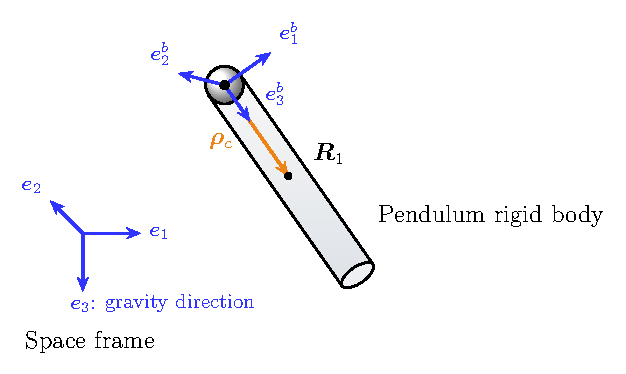
\includegraphics[width=0.75\textwidth]{pendulum_3d_so3.pdf}
	\caption{3D-pendulum system attached to a fixed pivot.}
	\label{fig:3d_pendulum}
\end{figure}

The 3D-Pendulum model, illustrated in \ref{fig:3d_pendulum}, consist of a rigid body rotating under the influence of gravity $g$ attached to a fixed frictionless pivot \cite{Shen20043DPendulum}. Moreover, the system has no external control moment, since it is unforced. A space frame and a body-fixed frame attached to the pendulum, both with their origins at the pivot, are defined. The unit vector $\bm{e}_3$ represents the gravity direction in the space frame, while $\bm{\rho_c}$ denotes the vector from the pivot to the center of mass expressed in the body-fixed frame. Following the fixed pivot, there is no translational degree of freedom. Therefore, the configuration manifold of the model is given by the special orthogonal group
\[
SO(3)
=
\left\{
\bm{R}\in\mathbb{R}^{3\times 3}
\;\middle|\;
\bm{R}^\top \bm{R}=\bm{I}_3,\ 
\det(\bm{R})=1
\right\}.\]
The configuration is completely determined by the rotation matrix $\bm{R}\in SO(3)$, which maps the body-fixed frame to the space frame. Additionally, in $SO(3)$ the attitude kinematics equation is defined by 
\begin{equation}
\label{eq:SO3_attitude_kinematics}
\dot{\bm{R}} = \bm{R}\hat{\bm{\omega}},
\end{equation}
with the angular velocity $\bm{\omega}\in \mathbb{R}^3$, mapped to the Lie algebra $\mathfrak{so}(3)$ by the hat map $\hat{\cdot}: \mathbb{R}^3 \to \mathfrak{so}(3)$ \cite{Lee2008}. Consequently, $\hat{\bm{\omega}}$ is a $3 \times 3$ skew-symmetric matrix. 

\paragraph{Lagrangian}

To derive the Lagrangian $L:SO(3) \times\mathfrak{so}(3) \to \mathbb{R}$, the kinetic $T:SO(3) \times\mathfrak{so}(3) \to \mathbb{R} $ and potential $V:SO(3) \to \mathbb{R}$ energy of the rigid body are introduced. The rotational inertia of the mass is expressed in the body-frame by the inertia matrix $\bm{J} \in \mathbb{R}^{3 \times 3}$. \cite{Lee2008} defines 
\begin{equation}\label{eq:3D_pendulum_kinetic_energy}
T(\bm{\omega}) = \frac{1}{2} \int_{B} \lVert \hat{\bm{\omega} \bm{\rho}} \rVert^{2} \, dm(\bm{\rho})
= \frac{1}{2}\operatorname{tr}[\hat{\bm{\omega}} \bm{J}_d \hat{\bm{\omega}}^\top]
= \frac{1}{2} \bm{\omega}^\top \bm{J} \bm{\omega},
\end{equation}
as a general expression for the kinetic energy of the single body $B$ with the velocity $\bm{\omega} \times \bm{\rho} = \hat{\bm{\omega}}\bm{\rho}$. Thereby, 
\begin{equation}\label{eq:non-standard_inertia}
    \bm{J}_d = \int_{B} \hat{\bm{\rho}} \hat{\bm{\rho}}^\top  \, dm(\bm{\rho})
    =\frac{1}{2}\operatorname{tr}[\bm{J}]\,\bm{I}-\bm{J},
\end{equation}
is a nonstandard inertia matrix, with the relation
\begin{equation} \label{eq:nonstandard_Inertia_Relation}
    (\bm{J}\bm{\omega})^\wedge = \hat{\bm{\omega}}\bm{J}_d + \bm{J}_d \hat{\bm{\omega}},
\end{equation}
for any $\bm{\omega}\in\mathbb{R}^3$. The potential energy is given by
\begin{equation}\label{eq:3D_pendulum_potential_energy}
    V(\bm{R}) = -mg\, \bm{e}_3^\top \bm{R}\bm{\rho}_c,
\end{equation}
where \(\bm{R}\bm{\rho}_c\) denotes the vector from the pivot to the center of mass expressed in the space-fixed frame, and \(\bm{e}_3^\top \bm{R}\bm{\rho}_c\) is its projection onto the gravity direction \(\bm{e}_3\) \cite{Lee2008}. Using \eqref{eq:3D_pendulum_kinetic_energy} and \eqref{eq:3D_pendulum_potential_energy}, the Lagrangian of the unforced 3D pendulum is given by 
\begin{equation}\label{eq:continuous_3D_pendulum_lagrangian}
    L(\bm{R}, \hat{\bm{\omega}}) = T(\hat{\bm{\omega}}) - V(\bm{R})
    = \frac{1}{2}\operatorname{tr}[\hat{\bm{\omega}} \bm{J}_d \hat{\bm{\omega}}^\top] + mg\, \bm{e}_3^\top \bm{R}\bm{\rho}_c.
\end{equation}


\paragraph{Euler--Lagrange Equations}

In order to define the Euler--Lagrange equations \eqref{eq:continuous_euler_lagrange_lie_group}, the derivatives of \eqref{eq:continuous_3D_pendulum_lagrangian} have to be calculated. Firstly, the directional derivative $D_{\hat{\bm{\omega}}}L(\bm{R},\hat{\bm{\omega}})$ is given by applying \eqref{eq:derivative_omega}, which yields
\begin{align}
\left\langle D_{\hat{\bm{\omega}}}L(\bm{R},\hat{\bm{\omega}}),\,\delta\hat{\bm{\omega}}\right\rangle
&=
\left.\frac{d}{d\epsilon}\right|_{\epsilon=0}
L\!\left(\bm{R},\hat{\bm{\omega}}+\epsilon\,\delta\hat{\bm{\omega}}\right) \notag\\
&=
\left.\frac{d}{d\epsilon}\right|_{\epsilon=0}
\frac{1}{2}\operatorname{tr}\!\left[
(\hat{\bm{\omega}}+\epsilon\,\delta\hat{\bm{\omega}})
\,\bm{J}_d\,
(\hat{\bm{\omega}}+\epsilon\,\delta\hat{\bm{\omega}})^{T}
\right] \notag\\
&=
\frac{1}{2}\operatorname{tr}\!\left[
\delta\hat{\bm{\omega}}\,\bm{J}_d\,\hat{\bm{\omega}}^{T}
+
\hat{\bm{\omega}}\,\bm{J}_d\,(\delta\hat{\bm{\omega}})^{T}
\right] \notag.
\end{align}
By using the antisymmetry identity of a cross product $\hat{\bm{x}}=-\hat{\bm{x}}^\top$ for any $\bm{x} \in \mathbb{R}^3$ and $\operatorname{tr}[\bm{A}\bm{B}]=\operatorname{tr}[\bm{B}\bm{A}]$ for any $\bm{A},\bm{B} \in \mathbb{R}^{3 \times 3}$, 
the directional derivative is rewritten as
\begin{align}\label{eq:continuous_3D_pendulum_derivative_omega}
\left\langle D_{\hat{\bm{\omega}}}L(\bm{R},\hat{\bm{\omega}}),\,\delta\hat{\bm{\omega}}\right\rangle
&=
\frac{1}{2}\operatorname{tr}\!\left[
-\delta\hat{\bm{\omega}}\,\bm{J}_d\,\hat{\bm{\omega}}
-
\hat{\bm{\omega}}\,\bm{J}_d\,\delta\hat{\bm{\omega}}
\right] \notag \\
&=
\frac{1}{2}\operatorname{tr}\!\left[
-\bigl(\bm{J}_d\hat{\bm{\omega}}+\hat{\bm{\omega}}\bm{J}_d\bigr)
\,\delta\hat{\bm{\omega}}
\right] \notag\\
&=
\left\langle \bm{J}_d\hat{\bm{\omega}}+\hat{\bm{\omega}}\bm{J}_d,\,
\delta\hat{\bm{\omega}}\right\rangle \notag\\
&=
\left\langle (\bm{J}\bm{\omega})^\wedge,\,\delta\hat{\bm{\omega}}\right\rangle,
\end{align}
with the definition of the inner product \eqref{eq:trace_inner_product} and the skew-symmetric property of \eqref{eq:nonstandard_Inertia_Relation}. 

\indent Moreover, the derivative $D_{\bm{R}}L(\bm{R},\hat{\bm{\omega}})$, which in this model depends only on the potential energy $V(\bm{R})$, is calculated using \eqref{eq:derivative_rotation} as
\begin{align}
\left\langle D_{\bm{R}} L(\bm{R},\hat{\bm{\omega}}),\,\delta \bm{R}\right\rangle
&=
\left\langle T_{e}^{*}\mathbb{L}_{\bm{R}}\,D_{\bm{R}} L(\bm{R},\hat{\bm{\omega}}),\, \hat{\bm{\eta}} \right\rangle \notag\\
&=
\left.\frac{d}{d\epsilon}\right|_{\epsilon=0}
L\!\left(\bm{R}\exp(\epsilon\hat{\bm{\eta}}),\hat{\bm{\omega}}\right) \notag\\
&=
\left.\frac{d}{d\epsilon}\right|_{\epsilon=0}
mg\,\bm{e}_3^{\top}\bm{R}\exp(\epsilon\hat{\bm{\eta}})\bm{\rho}_c \notag\\
&=
mg\,\bm{e}_3^{\top}\bm{R}\hat{\bm{\eta}}\,\bm{\rho}_c \notag\\
&=
mg\,(\bm{R}^{\top}\bm{e}_3)^{\top}\hat{\bm{\eta}}\,\bm{\rho}_c \notag\\
&=
mg\,(\bm{\rho}_c\times \bm{R}^{\top}\bm{e}_3)\cdot \bm{\eta}, \notag
\end{align}
since $\bm{a}^\top \hat{\bm{x}}\bm{b} = \bm{a} \cdot(\bm{x} \times \bm{b}) = (\bm{b} \times \bm{a}) \cdot \bm{x}$ for any $\bm{a}, \bm{b}, \bm{x} \in \mathbb{R}^3$. Applying the definition of inner products \eqref{eq:trace_inner_product}, it follows that 
\begin{equation}\label{eq:continuous_3D_pendulum_derivative_rotation}
    \left\langle T_{e}^{*}\mathbb{L}_{\bm{R}}\,D_{\bm{R}} L(\bm{R},\hat{\bm{\omega}}),\, \hat{\bm{\eta}} \right\rangle
    = \left\langle (mg\,(\bm{\rho}_c\times \bm{R}^{\top}\bm{e}_3))^\wedge, \hat{\bm{\eta}}\right\rangle.
\end{equation}

Since the directional derivative
\[
D_{\hat{\bm{\omega}}}L(\bm{R},\hat{\bm{\omega}})
\;\widehat{=}\;
\bm{J}_d\hat{\bm{\omega}}+\hat{\bm{\omega}}\bm{J}_d,
\]
was derived in \eqref{eq:continuous_3D_pendulum_derivative_omega}, the coadjoint term in the Euler--Lagrange equations can be written in matrix form by using the identity \eqref{eq:ad_lie_bracket}. Therefore,
\begin{align}
ad^*_{\hat{\bm{\omega}}}D_{\hat{\bm{\omega}}}L(\bm{R},\hat{\bm{\omega}})
&=
\left[\bm{J}_d\hat{\bm{\omega}}+\hat{\bm{\omega}}\bm{J}_d,\hat{\bm{\omega}}\right] \notag \\
&=
(\bm{J}_d\hat{\bm{\omega}}+\hat{\bm{\omega}}\bm{J}_d)\hat{\bm{\omega}}
-
\hat{\bm{\omega}}(\bm{J}_d\hat{\bm{\omega}}+\hat{\bm{\omega}}\bm{J}_d) \notag \\
&=
(\bm{J}\bm{\omega} \times \bm{\omega})^\wedge \notag
\end{align}
with the relation $\hat{\bm{x}}\hat{\bm{y}}-\hat{\bm{y}}\hat{\bm{x}}=(\bm{x} \times \bm{y})^\wedge$ for any $\bm{x},\bm{y} \in \mathbb{R}^3$ and \eqref{eq:nonstandard_Inertia_Relation}. Furthermore, by the antisymmetry of the cross product, it follows that
\begin{equation} \label{eq:continuous_3D_pendulum_adjoint_derivative_omega}   
ad^*_{\hat{\bm{\omega}}}D_{\hat{\bm{\omega}}}L(\bm{R},\hat{\bm{\omega}})
= (\bm{J}\bm{\omega} \times \bm{\omega})^\wedge
= -(\bm{\omega} \times \bm{J} \bm{\omega})^\wedge
\end{equation}
\indent Finally, the Euler-Lagrange equations of the unforced 3D-pendulum are expressed in $\mathfrak{so}(3)$ and $SO(3)$ form, by substituting \eqref{eq:continuous_3D_pendulum_derivative_omega}, \eqref{eq:continuous_3D_pendulum_derivative_rotation} and \eqref{eq:continuous_3D_pendulum_adjoint_derivative_omega} into \eqref{eq:continuous_euler_lagrange_lie_group}, which results in
\begin{subequations}\label{eq:continuous_3D_pendulum_euler_lagrange}
\begin{align}
 (\bm{J}\dot{\bm{\omega}})^\wedge + (\bm{\omega}\times (\bm{J}\bm{\omega}))^\wedge
 &= (mg\,\bm{\rho}_c \times \bm{R}^T\bm{e}_3)^\wedge,
 \label{eq:continuous_3D_pendulum_euler_lagrange_dynamics} \\
 \dot{\bm{R}} &= \bm{R}\hat{\bm{\omega}}.
 \label{eq:continuous_3D_pendulum_euler_lagrange_kinematics}
\end{align}
\end{subequations}

\paragraph{Legendre Transformation}

In order to obtain Hamilton's equations for the unforced 3D-pendulum model, the Legendre transformation $\mathbb{F}L:(SO(3)\times\mathfrak{so}(3)) \to (SO(3) \times \mathfrak{so}(3)^*)$ \eqref{eq:continuous_generalized_momentum} has to be applied, which results in the expression for the momentum
\begin{equation}  \label{eq:continuous_3D_pendulum_momentum}
    \hat{\bm{\Pi}} = D_{\hat{\bm{\omega}}}L(\bm{R},\hat{\bm{\omega}}) = (\bm{J}\bm{\omega})^\wedge
\end{equation}
where $ \hat{\bm{\Pi}} \in \mathfrak{so}(3)^*$. By substituting \eqref{eq:continuous_3D_pendulum_momentum} into \eqref{eq:continuous_3D_pendulum_euler_lagrange}, Hamilton's equations of an unforced 3D-pendulum are 
\begin{subequations}\label{eq:continuous_3D_pendulum_hamilton}
\begin{align}
    \hat{\dot{\bm{\Pi}}} + (\bm{J}^{-1}\bm{\Pi} \times \bm{\Pi})^\wedge &= (mg\,\bm{\rho}_c \times \bm{R}^T \bm{e}_3)^\wedge,
    \label{eq:continuous_3D_pendulum_hamilton_momentum} \\
    \dot{\bm{R}} &= \bm{R}(\bm{J}^{-1}\bm{\Pi})^\wedge,
    \label{eq:continuous_3D_pendulum_hamilton_kinematics}
\end{align}
\end{subequations}
with $\bm{J}$ being nonsingular.
Finally, the derived Euler-Lagrange equations \eqref{eq:continuous_3D_pendulum_euler_lagrange} and Hamilton's equations \eqref{eq:continuous_3D_pendulum_hamilton} correspond to the given 3D-pendulum results of \cite{Lee2008}.

\subsection{Verification of Momentum Conservation}
\label{sec:continuous_3D_pendulum_momentum_validation}


The verification of momentum conservation is particularly relevant,
in order to ensure that the numerical integration of the system's dynamics preserves the physical properties of the system over long time. 
This is essential for accurate numerical simulation and for 
reliable trajectory optimization methods \cite{Sangli2025}. Therefore, in the following, the momentum conservation property of the continuous 3D pendulum is verified based on its symmetry and Noether's theorem \ref{thm:continuous_noether}.

\cite{Lee2008} identifies a symmetry of the unforced 3D-pendulum's Lagrangian, which is infinitesimally invariant under an action of the group $H = SO(2) \simeq S^1$. Here, a rotation about the gravity direction $\bm{e}_3$ does not change the Lagrangian. Thus, $SO(2)$ and $S^1$ describe the same symmetry group under the left action $\Phi: S^1 \times SO(3) \to SO(3)$ of $H$ on $G$,
\begin{equation}\label{eq:continuous_3D_pendulum_symmetry_action}
    \Phi(\theta, \bm{R})= \exp_{SO(3)}(\theta \hat{\bm{e}_3})\bm{R},
\end{equation}
where $\exp_{SO(3)}(\theta \hat{\bm{e}_3})$ expresses a finite rotation about the gravity direction $\bm{e}_3$ by the angle $\theta$ \cite{Lee2008}. By Noether's Theorem \ref{thm:continuous_noether}, the infinitesimal invariance of the 3D-pendulum's Lagrangian is verified, if 
\begin{equation}\label{eq:continuous_3D_momentum_conservation}
    dL(\bm{R},\hat{\bm{\omega}})\cdot \zeta_{SO(3)\times\mathfrak{so}(3)}(\bm{R}, \hat{\bm{\omega}}) = 0.
\end{equation}
Consequently, preserving the Lagrangian momentum map along the flow $J_L\!\left(\mathcal{F}_L^T(\bm{R},\hat{\bm{\omega}})\right)=J_L(\bm{R},\hat{\bm{\omega}})$.

Therefore, the infinitesimal generator of the lifted group action on $SO(3)\times\mathfrak{so}(3)$ is required \cite{Lee2008}. With the attitude kinematics relation \eqref{eq:SO3_attitude_kinematics}, the left trivialization $\phi_L(\bm{R},\dot{\bm{R}})=\phi_L(\bm{R},\bm{R}\hat{\bm{\omega}})=(\bm{R},T_e\mathbb{L}_{\bm{R}^{-1}}\bm{R}\hat{\bm{\omega}})=(\bm{R},\hat{\bm{\omega}})$, and its inverse $\phi_L^{-1}(\bm{R},\hat{\bm{\omega}})=(\bm{R},T_e\mathbb{L}_{\bm{R}}\hat{\bm{\omega}})=(\bm{R},\bm{R}\hat{\bm{\omega}})$ are taken from \eqref{eq:left_trivialization_noethers_theorem}, with the differential $T_{\bm{R}}$ of \eqref{eq:preliminaries_differential_left_SO}. Following \cite{Lee2008}, the lifted infinitesimal generator $\zeta_{SO(3) \times \mathfrak{so}(3)}:SO(3) \times \mathfrak{so}(3) \to T(SO(3) \times \mathfrak{so}(3))$ \eqref{eq:lifted_infinitesimal_generator} is computed as
\begin{align}
\zeta_{SO(3)\times\mathfrak{so}(3)}(\bm{R},\hat{\bm{\omega}})
&=
\left.\frac{d}{d\epsilon}\right|_{\epsilon=0}
\phi_L \circ T_{\bm{R}}\Phi_{\exp_{SO(2)}(\epsilon\zeta)}
\circ \phi_L^{-1}(\bm{R},\hat{\bm{\omega}}) \notag\\
&=
\left.\frac{d}{d\epsilon}\right|_{\epsilon=0}
\phi_L \circ T_{\bm{R}}\Phi_{\exp_{SO(2)}(\epsilon\zeta)}
(\bm{R},\bm{R}\hat{\bm{\omega}}) \notag\\
&=
\left.\frac{d}{d\epsilon}\right|_{\epsilon=0}
\phi_L\!\left(
\exp(\epsilon\zeta\hat{\bm{e}}_3)\bm{R},
\exp(\epsilon\zeta\hat{\bm{e}}_3)\bm{R}\hat{\bm{\omega}}
\right) \notag\\
&=
\left.\frac{d}{d\epsilon}\right|_{\epsilon=0}
\left(
\exp(\epsilon\zeta\hat{\bm{e}}_3)\bm{R},
\bm{R}^{-1}\exp(\epsilon\zeta\hat{\bm{e}}_3)^{-1}
\bigl(\exp(\epsilon\zeta\hat{\bm{e}}_3)\bm{R}\hat{\bm{\omega}}\bigr)
\right) \notag\\
&=
\left.\frac{d}{d\epsilon}\right|_{\epsilon=0}
\left(
\exp(\epsilon\zeta\hat{\bm{e}}_3)\bm{R},
\hat{\bm{\omega}}
\right) \notag\\
&=
\left(
\zeta\hat{\bm{e}}_3\bm{R},
\bm{0}
\right).
\label{eq:continuous_3D_pendulum_lifted_generator}
\end{align}

This result can be substituted into \eqref{eq:continuous_3D_momentum_conservation}, using \eqref{eq:continuous_3D_pendulum_derivative_rotation}, which gives
\begin{align}
dL(\bm{R},\hat{\bm{\omega}})\cdot
\zeta_{SO(3)\times\mathfrak{so}(3)}(\bm{R},\hat{\bm{\omega}})
&=
dL(\bm{R},\hat{\bm{\omega}})\cdot
(\zeta \hat{\bm{e}}_3\bm{R},\bm{0}) \notag\\
&=
\left\langle D_{\bm{R}}L(\bm{R},\hat{\bm{\omega}}),\,\zeta \hat{\bm{e}}_3\bm{R}\right\rangle
+
\left\langle D_{\hat{\bm{\omega}}}L(\bm{R},\hat{\bm{\omega}}),\,\bm{0}\right\rangle \notag\\
&=
\left\langle T_e^*\mathbb{L}_{\bm{R}}D_{\bm{R}}L(\bm{R},\hat{\bm{\omega}}),\,
\hat{\bm{\eta}}\right\rangle.
\label{eq:continuous_3D_pendulum_infinitesimal_invariance_start}
\end{align}
Since the lifted generator has no component in the $\hat{\bm{\omega}}$ direction, the component directional derivative $D_{\hat{\bm{\omega}}}$ equals zero in the zero direction. Moreover, by the definition of the lifted infinitesimal generator \eqref{eq:lifted_infinitesimal_generator}, the result of \eqref{eq:continuous_3D_pendulum_lifted_generator} redefines the variational relationship as
\begin{equation} \label{eq:continuous_3D_pendulum_lifted_action_generator_variation}
    (\delta \bm{R}, \delta \hat{\bm{\omega}}) = (\zeta \hat{\bm{e}}_3\bm{R},\bm{0}).
\end{equation}
Consequently, using the previously given infinitesimal variation \eqref{eq:continuous_lie_group_variations}, the corresponding relation $\delta \bm{R} = \zeta \hat{\bm{e}}_3 \bm{R} = \bm{R} \hat{\bm{\eta}}$ is defined, from which the variation $\hat{\bm{\eta}}$ can be expressed as
\begin{equation}\label{eq:continuous_3D_pendulum_variation_eta}
    \hat{\bm{\eta}}= \zeta \bm{R}^{-1} \hat{\bm{e}}_3 \bm{R}.
\end{equation}
This can be substituted into \eqref{eq:continuous_3D_pendulum_infinitesimal_invariance_start}, yielding
\begin{align}
\left\langle T_e^*\mathbb{L}_{\bm{R}}D_{\bm{R}}L(\bm{R},\hat{\bm{\omega}}),\,
\zeta \bm{R}^{-1}\hat{\bm{e}}_3\bm{R}\right\rangle
&=
\left.\frac{d}{d\epsilon}\right|_{\epsilon=0}
L\!\left(\bm{R}\exp\!\left(\epsilon \zeta \bm{R}^{-1}\hat{\bm{e}}_3\bm{R}\right),\hat{\bm{\omega}}\right).
\notag
\end{align}
Since only the potential term of the 3D-pendulum $V(\bm{R})$ \eqref{eq:3D_pendulum_potential_energy} depends on $\bm{R}$ and \eqref{eq:continuous_3D_pendulum_variation_eta} is skew symmetric, it can be shown that 
\begin{align} \label{eq:continuous_3d_pendulum_validation}
\left.\frac{d}{d\epsilon}\right|_{\epsilon=0}
L\!\left(\bm{R}\exp\!\left(\epsilon \zeta \bm{R}^{-1}\hat{\bm{e}}_3\bm{R}\right),\hat{\bm{\omega}}\right)
&=
mg\,\bm{e}_3^T\bm{R}
\left(\zeta \bm{R}^{-1}\hat{\bm{e}}_3\bm{R}\right)
\bm{\rho}_c \notag\\
&=
mg\,(\bm{\rho}_c^\top
\left(\zeta \bm{R}^{-1}\hat{\bm{e}}_3\bm{R}\right)^\top
\bm{R}^\top\bm{e}_3)^\top \notag\\
&=
-\,mg\,\bm{\rho}_c^\top
\left(\zeta \bm{R}^{-1}\hat{\bm{e}}_3\bm{R}\right)
\bm{R}^\top\bm{e}_3 \notag\\
&=
-\,mg\,\bm{\rho}_c^\top
\zeta \bm{R}^{-1}\hat{\bm{e}}_3\bm{e}_3 \notag\\
&=
-\,mg\,\bm{\rho}_c^\top
\zeta \bm{R}^{-1}(\bm{e}_3\times \bm{e}_3) \notag\\
&=0,
\end{align}
because $\bm{e}_3\times \bm{e}_3=\bm{0}$ and $\bm{R}^{-1}=\bm{R}^{\top}$ for any $\bm{R} \in SO(3)$. Therefore, the condition of \eqref{eq:continuous_3D_momentum_conservation} is verified and the Lagrangian is infinitesimally invariant under the symmetry action. Consequently, by Noether's Theorem ~\ref{thm:continuous_noether}, 
the corresponding momentum map $J_L(\bm{R},\bm{\omega})$ of the continuous 3D-pendulum is preserved along the Lagrangian flow
\[  J_L\!\left(\mathcal{F}_L^T(\bm{R},\hat{\bm{\omega}})\right)
    =
    J_L(\bm{R},\hat{\bm{\omega}}).
\]

\chapter{Discrete Mechanics for Rigid Bodies on Lie Groups}
\label{chapter:discrete_mechanics_for_rigid_bodies_on_lie_groups}

This chapter introduces the discrete mechanics of rigid bodies on Lie groups
for trajectory optimization computations. Thereby, it is the discrete-time 
version of the continuous mechanics in Chapter~\ref{chapter:continous_mechanics_of_rigid_bodies_on_lie_groups}. 
Instead of applying standard numerical integration methods, for example, 
the midpoint or trapezoidal rule, directly to the 
continuous equations of motion, variational integrators discretize Hamilton's 
principle. Therefore, the resulting discrete flow 
preserves the variational and geometric structure of the mechanical system 
\cite{Marsden2001,Leimkuhler_Reich_2005}. 
In correspondence with \cite{Lee2008}, the discrete time nodes 
are defined by
\begin{align*}
    t_k=t_0+kh,
    \qquad
    k=0,\ldots,N, 
    \qquad
    \text{and}
    \qquad
    Nh=t_f-t_0,
    \label{eq:discrete_time_grid}
\end{align*}
for a fixed time step $h>0$ and $N$ time steps.

Section~\ref{sec:discrete_lagrangian_mechanics} introduces the forced discrete
Euler-Lagrange equations, including the discrete Legendre transformation, and the 
geometric properties of the discrete Lagrangian flow. Additionally, a computational
approach is given for solving the implicit discrete equations. 
Subsequently, in Section \ref{sec:single_rigid_body_systems}, the formulation 
is applied to a single rigid body system and extended to 
multi-body systems in maximal coordinates in Section \ref{sec:multi_body_systems}. 
These discrete models are used for the geometric trajectory optimization
formulation and computation in 
Chapter~\ref{chapter:certifiable_trajectory_optimization}.

\section{Discrete Lagrangian Mechanics}
\label{sec:discrete_lagrangian_mechanics}

Following the continuous Lagrangian mechanics in 
Chapter \ref{chapter:continous_mechanics_of_rigid_bodies_on_lie_groups}, 
discrete Lagrangian mechanics is based on the discrete variational principle.
The continuous trajectory is replaced by 
a sequence of configurations on the Lie group, and the action integral is 
approximated by an action sum. For a regular discrete Lagrangian, the resulting Lie group 
variational integrator defines a symplectic discrete flow that remains on the configuration 
manifold. If the discrete Lagrangian is invariant under a lifted Lie-group action, the 
associated discrete 
momentum map is preserved exactly at every time step 
manifold \cite{Marsden2001,Lee2008}.

Figure~\ref{fig:discrete_mechanics} summarizes the general method for deriving the 
discrete Euler--Lagrange equations of a mechanical system on a Lie group.
Thereby, the discrete Euler-Lagrange equations are obtained from the variation
of the action sum. Alternatively, the discrete Legendre transformation can be used
to derive the discrete Hamiltonian equations of motion.

\begin{figure}[ht]
    \centering
    \resizebox{\textwidth}{!}{%
    \begin{tikzpicture}[
        node distance=0.9cm and 1.2cm,
        box/.style={
            draw, rectangle, align=center, minimum width=4.8cm,
            minimum height=1.2cm, inner sep=6pt
        },
        arrow/.style={-Latex}
    ]
        \node[box] (manifold) {Discrete configuration state\\ $(\bm{g}_k,\bm{f}_k)\in G\times G$};
        \node[box, below=of manifold] (lagrangian) {Discrete Lagrangian\\ $L_d(\bm{g}_k,\bm{f}_k)$};
        \node[box, below left=of lagrangian, xshift=1.3cm, yshift=-0.3cm] (action) {Action sum\\ $\mathcal S_d=\sum_{k=0}^{N-1}L_d(\bm{g}_k,\bm{f}_k)$};
        \node[box, below right=of lagrangian, xshift=-1.3cm, yshift=-0.3cm] (legendre) {Discrete Legendre transforms\\ $\bm{\mu}_k = \mathbb{F} L_d(\bm{g}_k,\bm{f}_k)$};
        \node[box, below=of action] (variation) {Variation\\ $\delta\mathcal S_d=0$};
        \node[box, below=of legendre] (hamilton) {Discrete Hamilton equations};
        \node[box, below=of variation] (euler) {Discrete Euler--Lagrange equations};

        \draw[arrow] (manifold) -- (lagrangian);
        \draw[arrow] (lagrangian) -- (action);
        \draw[arrow] (lagrangian) -- (legendre);
        \draw[arrow] (action) -- (variation);
        \draw[arrow] (legendre) -- (hamilton);
        \draw[arrow] (variation) -- (euler);
    \end{tikzpicture}%
    }
    \caption{General method to derive the discrete Euler--Lagrange equations of a mechanical system on a Lie group. Adapted from \cite{Lee2008}.}
    \label{fig:discrete_mechanics}
\end{figure}

\subsection{Discrete Euler--Lagrange Equations}
\label{sec:discrete_euler_lagrange_equations}

Following \cite{Lee2008,Marsden2001}, $G$ is a matrix Lie group with Lie algebra $\mathfrak g$. 
Thereby, a discrete trajectory $\bm{g}_d$ is defined by a sequence of configurations 
$\{\bm{g}_k\}_{k=0}^{N}$, where $\bm{g}_k = \bm{g}_d(t_k)$. The discrete state space is defined on $G \times G$.
By defining the relative group element $\bm{f}_k\in G$, the discrete-time kinematic equation is given by
\begin{equation}
    \bm{g}_{k+1}=\bm{g}_k\bm{f}_k.
    \label{eq:discrete_lie_group_kinematics}
\end{equation}
Consequently, the multiplicative update guarantees that $\bm{g}_{k+1}\in G$.

The discrete Lagrangian $L_d:G\times G\rightarrow\mathbb R$
approximates the action integral of the continuous Lagrangian over the interval $[t_k,t_{k+1}]$.
\cite{Marsden2001} states that, for sufficiently small $h$ and a regular continuous Lagrangian, the exact discrete Lagrangian is defined by
\begin{equation}
    L_d^{\mathrm{exact}}(\bm{g}_k,\bm{f}_k)
    =
    \int_0^h
    L\!\left(\widetilde{\bm{g}}(t),
    \widetilde{\bm{g}}(t)^{-1}\dot{\widetilde{\bm{g}}}(t)\right)
    \,\mathrm dt,
    \label{eq:exact_discrete_lagrangian}
\end{equation}
with the boundary conditions $\widetilde{\bm{g}}(0)=\bm{g}_k, \widetilde{\bm{g}}(h)=\bm{g}_k\bm{f}_k$.
Moreover, $\widetilde{\bm{g}}:[0,h]\rightarrow G$ satisfies the continuous Euler-Lagrange 
equations \eqref{eq:continuous_euler_lagrange_lie_group} \cite{Lee2008}. 
However, in this thesis, $L_d$ is calculated using the trapezoidal rule \eqref{eq:trapezodial_rule} 
to approximate \eqref{eq:exact_discrete_lagrangian}.

The discrete action sum is given by
\begin{equation}
    \mathcal S_d
    =
    \sum_{k=0}^{N-1}L_d(\bm{g}_k,\bm{f}_k).
    \label{eq:discrete_action_sum}
\end{equation}
Similarly to the continuous action integral \eqref{eq:hamilton_principle_lie_group} and the variation of the continuous Lagrangian \eqref{eq:variation_continuous_lagrangian}, 
the discrete Hamilton principle states that the action sum is stationary
\begin{equation}
    \delta\mathcal S_d
    =
    \sum_{k=0}^{N-1}\delta L_d(\bm{g}_k,\bm{f}_k)
    = \sum_{k=0}^{N-1} \left\langle D_{\bm{g}_k}L_d(\bm{g}_k,\bm{f}_k),\delta\bm{g}_k\right\rangle
    +
    \left\langle D_{\bm{f}_k}L_d(\bm{g}_k,\bm{f}_k),\delta\bm{f}_k\right\rangle
    =0,
    \label{eq:discrete_hamilton_principle}
\end{equation}
for all possible variations of $\bm{g}_d$ with fixed endpoints at $k=0$ and $k=N$ \cite{Marsden2001}.

Analogously to the continuous variation in \eqref{eq:continuous_curve_variation_lie_group}, 
the variation of the discrete configuration sequence is defined by
\begin{equation}
    \bm{g}_k^{\epsilon}
    =
    \bm{g}_k\exp(\epsilon\bm{\eta}_k)
    \label{eq:discrete_configuration_variation}
\end{equation}
with the discrete matrix-valued curve $\{\bm{\eta}_k \}^N_{k=0}$ and $\bm{\eta}_0=\bm{\eta}_N=\bm{0}$ \cite{Lee2008}.
Using the infinitesimal variation introduced 
in \eqref{eq:infinitesimal_variation_matrix_lie_group}, it follows that
\begin{equation}
    \delta\bm{g}_k=\bm{g}_k\bm{\eta}_k=T_e\mathbb{L}_{\bm{g}_k}(\bm{\eta}_k).
    \label{eq:discrete_infinitesimal_configuration_variation}
\end{equation}
Moreover, \cite{Lee2008} derives the infinitesimal variation of $\bm{f}_k$ as
\begin{align}
    \delta\bm{f}_k
    =
    T_e\mathbb{L}_{\bm{f}_k} \cdot \left(
        -\operatorname{Ad}_{\bm{f}_k^{-1}}\bm{\eta}_k+\bm{\eta}_{k+1}
    \right)
    =\bm{f}_k\bm{X}_k,
    \label{eq:discrete_relative_group_variation}
\end{align}
with $\bm{X}_k = -\operatorname{Ad}_{\bm{f}_k^{-1}}\bm{\eta}_k+\bm{\eta}_{k+1} \in\mathfrak g$.
After substituting \eqref{eq:discrete_infinitesimal_configuration_variation} and 
\eqref{eq:discrete_relative_group_variation} into \eqref{eq:discrete_hamilton_principle},
the variation of the action sum becomes 
\begin{align}
    \delta\mathcal S_d
    =
    \sum_{k=1}^{N-1}
    \Big\langle
        &T_e^*\mathbb{L}_{\bm{f}_{k-1}} \cdot D_{\bm{f}_{k-1}}L_d(\bm{g}_{k-1},\bm{f}_{k-1})
        +T_e^*\mathbb{L}_{\bm{g}_k} \cdot D_{\bm{g}_k}L_d(\bm{g}_k,\bm{f}_k)
        \notag\\
        &-
        \operatorname{Ad}_{\bm{f}_k^{-1}}^* \cdot
        \left(T_e^*\mathbb{L}_{\bm{f}_k} \cdot D_{\bm{f}_k}L_d(\bm{g}_k,\bm{f}_k)\right),
        \bm{\eta}_k
    \Big\rangle
    =0,
    \label{eq:variation_discrete_action_sum}
\end{align}
shifting the summation index, and using $\bm{\eta}_0=\bm{\eta}_N=\bm{0}$ \cite{Lee2008}.

Since \eqref{eq:variation_discrete_action_sum} holds for all 
sequences $\{\bm{\eta}_k\}_{k=1}^{N-1}\subset\mathfrak g$, the discrete Euler-Lagrange 
equations on $G$ are defined as
\begin{subequations}
\label{eq:discrete_euler_lagrange_lie_group}
\begin{align}
    T_e^*\mathbb{L}_{\bm{f}_{k-1}} \cdot D_{\bm{f}_{k-1}}L_d(\bm{g}_{k-1},\bm{f}_{k-1})
    &-
    \operatorname{Ad}_{\bm{f}_k^{-1}}^* \cdot
    \left(T_e^*\mathbb{L}_{\bm{f}_k} \cdot D_{\bm{f}_k}L_d(\bm{g}_k,\bm{f}_k)\right)
    \notag\\
    &+
    T_e^*\mathbb{L}_{\bm{g}_k} \cdot D_{\bm{g}_k}L_d(\bm{g}_k,\bm{f}_k)
    =0,
    \label{eq:discrete_euler_lagrange_balance}\\
    \bm{g}_{k+1}&=\bm{g}_k\bm{f}_k,
    \label{eq:discrete_euler_lagrange_reconstruction}
\end{align}
\end{subequations}
\cite{Lee2008}.
Equation~\eqref{eq:discrete_euler_lagrange_balance} is the dynamical representation of the
system in the body-fixed frame, while 
\eqref{eq:discrete_euler_lagrange_reconstruction} updates 
the configuration on the Lie group. 

In order to derive the discrete Euler-Lagrange equations in the following sections, 
the definitions of the partial derivatives $D_{\bm{g}_k}L_d(\bm{g}_k,\bm{f}_k)$ and $D_{\bm{f}_k}L_d(\bm{g}_k,\bm{f}_k)$ are required. 

\begin{proposition}[Directional derivative representation of $D_{\bm{g}_k}L_d(\bm{g}_k,\bm{f}_k)$]
\label{prop:directional_derivative_discrete_g}
Let $G$ be a Lie group with Lie algebra $\mathfrak g$, and let $L_d:G\times G\rightarrow\mathbb R$ be smooth \cite{Hall2000LieGroups}. 
For any $\delta\bm{g}_k=T_e\mathbb{L}_{\bm{g}_k}(\bm{\eta}_k)=\bm{g}_k\bm{\eta}_k \in T_{\bm{g}_k}G$ \eqref{eq:discrete_infinitesimal_configuration_variation}, the partial derivative $D_{\bm{g}_k}L_d(\bm{g}_k,\bm{f}_k)\in T_{\bm{g}_k}^*G$ is characterized by
\begin{equation}
    \left\langle D_{\bm{g}_k}L_d(\bm{g}_k,\bm{f}_k),\delta\bm{g}_k\right\rangle
    =
    \left\langle T_e^*\mathbb{L}_{\bm{g}_k} \cdot D_{\bm{g}_k}L_d(\bm{g}_k,\bm{f}_k),\bm{\eta}_k\right\rangle
    =
    \left.\frac{\mathrm d}{\mathrm d\epsilon}\right|_{\epsilon=0}
    L_d\!\left(\bm{g}_k\exp(\epsilon\bm{\eta}_k),\bm{f}_k\right).
    \label{eq:directional_derivative_discrete_g}
\end{equation}
\end{proposition}

\begin{proof}
By definition of the infinitesimal variation $\bm{g}_k^\epsilon$ \eqref{eq:discrete_infinitesimal_configuration_variation} and the definition of the infinitesimal 
variation on matrix Lie groups \eqref{eq:infinitesimal_variation_matrix_lie_group}, the corresponding directional derivative is
\begin{equation*}
    \left\langle D_{\bm{g}_k}L_d(\bm{g}_k,\bm{f}_k),\delta\bm{g}_k\right\rangle
    =
    \left.\frac{\mathrm d}{\mathrm d\epsilon}\right|_{\epsilon=0}
    L_d\!\left(\bm{g}_k\exp(\epsilon\bm{\eta}_k),\bm{f}_k\right).
\end{equation*}
using $\left\langle D_{\bm{g}_k}L_d(\bm{g}_k,\bm{f}_k),\delta\bm{g}_k\right\rangle = D_{\bm{g}_k}L_d(\bm{g}_k,\bm{f}_k)(\delta\bm{g}_k)$.
Additionally, the directional derivative can be expressed by the covector $T_e^*\mathbb{L}_{\bm{g}_k}$ and the definition of the differential 
of the left translation $\bm{g}_k \bm{\eta}_k = T_e\mathbb{L}_{\bm{g}_k}(\bm{\eta}_k)$ defined in \eqref{eq:preliminaries_differential_left_translation}, which leads to
\begin{align*}
    \left\langle D_{\bm{g}_k}L_d(\bm{g}_k,\bm{f}_k),\delta\bm{g}_k\right\rangle
    &=
    \left\langle D_{\bm{g}_k}L_d(\bm{g}_k,\bm{f}_k),\bm{g}_k \bm{\eta}_k\right\rangle \\
    &=
    \left\langle D_{\bm{g}_k}L_d(\bm{g}_k,\bm{f}_k),T_e\mathbb{L}_{\bm{g}_k}(\bm{\eta}_k)\right\rangle \\
    &=
    \left\langle T_e^*\mathbb{L}_{\bm{g}_k} \cdot D_{\bm{g}_k}L_d(\bm{g}_k,\bm{f}_k),\bm{\eta}_k\right\rangle.
\end{align*}
\end{proof}

\begin{proposition}[Directional derivative representation of $D_{\bm{f}_k}L_d(\bm{g}_k,\bm{f}_k)$]
\label{prop:directional_derivative_discrete_f}
Let $G$ be a matrix Lie group with Lie algebra $\mathfrak g$, 
and let $L_d:G\times G\rightarrow\mathbb R$ be smooth \cite{Hall2000LieGroups}. 
For any $\delta\bm{f}_k=T_e\mathbb{L}_{\bm{f}_k}(\bm{X}_k)=\bm{f}_k\bm{X}_k\in T_{\bm{f}_k}G$ \eqref{eq:discrete_relative_group_variation}, 
the partial derivative $D_{\bm{f}_k}L_d(\bm{g}_k,\bm{f}_k)\in T_{\bm{f}_k}^*G$ is characterized by
\begin{align}
    \left\langle D_{\bm{f}_k}L_d(\bm{g}_k,\bm{f}_k),\delta\bm{f}_k\right\rangle
    &=
    \left\langle T_e^*\mathbb{L}_{\bm{f}_k} \cdot D_{\bm{f}_k}L_d(\bm{g}_k,\bm{f}_k),\bm{X}_k\right\rangle
    \notag\\
    &=
    \left.\frac{\mathrm d}{\mathrm d\epsilon}\right|_{\epsilon=0}
    L_d\!\left(\bm{g}_k,\bm{f}_k\exp(\epsilon \bm{X}_k)\right).
    \label{eq:directional_derivative_discrete_f}
\end{align}
\end{proposition}

\begin{proof}
By definition of the infinitesimal variation $\bm{f}_k^\epsilon$ \eqref{eq:discrete_relative_group_variation} and the definition of the infinitesimal 
variation on matrix Lie groups \eqref{eq:infinitesimal_variation_matrix_lie_group}, 
the corresponding directional derivative is
\begin{equation*}
    \left\langle D_{\bm{f}_k}L_d(\bm{g}_k,\bm{f}_k),\delta\bm{f}_k\right\rangle
    =
    \left.\frac{\mathrm d}{\mathrm d\epsilon}\right|_{\epsilon=0}
    L_d\!\left(\bm{g}_k,\bm{f}_k\exp(\epsilon \bm{X}_k)\right).
\end{equation*}
using $\left\langle D_{\bm{f}_k}L_d(\bm{g}_k,\bm{f}_k),\delta\bm{f}_k\right\rangle = D_{\bm{f}_k}L_d(\bm{g}_k,\bm{f}_k)(\delta\bm{f}_k)$.
Additionally, the directional derivative can be expressed by the covector $T_e^*\mathbb{L}_{\bm{f}_k}$ and the
definition of the differential of the left translation $\bm{f}_k \bm{X}_k = T_e\mathbb{L}_{\bm{f}_k}(\bm{X}_k)$ 
defined in \eqref{eq:preliminaries_differential_left_translation}, which leads to 
\begin{align*}    
\langle D_{\bm{f}_k}L_d(\bm{g}_k,\bm{f}_k),\delta\bm{f}_k\rangle
&= \langle D_{\bm{f}_k}L_d(\bm{g}_k,\bm{f}_k),\bm{f}_k \bm{X}_k \rangle \\
&= \langle D_{\bm{f}_k}L_d(\bm{g}_k,\bm{f}_k), T_e\mathbb{L}_{\bm{f}_k}(\bm{X}_k) \rangle \\
&= \langle T_e ^* \mathbb{L}_{\bm{f}_k} \cdot D_{\bm{f}_k}L_d(\bm{g}_k,\bm{f}_k), \bm{X}_k \rangle.
\end{align*}
\end{proof}

\subsection{Discrete Legendre Transformation and Hamiltonian Mechanics}
\label{sec:discrete_legendre_hamiltonian_mechanics}

Correspondingly to the continuous Legendre transformation in Section~\ref{sec:continuous_legendre_hamiltonian_mechanics}, the same discrete dynamics can be represented on the left-trivialized cotangent bundle $T^*G$ 
identified with $G\times\mathfrak g^*$. Thereby, \cite{Lee2008} defines the discrete Legendre 
transformations $\mathbb{F}^+L_d, \mathbb{F}^- L_d: G \times G \to G \times \mathfrak{g}^*$ 
as
\begin{subequations}
\label{eq:discrete_legendre_transformations}
\begin{align}
    \mathbb F^+L_d(\bm{g}_k,\bm{f}_k)
    &=
    (\bm{g}_k\bm{f}_k,\bm{\mu}_{k+1}),
    \label{eq:positive_discrete_legendre_transformation}\\
    \mathbb F^-L_d(\bm{g}_k,\bm{f}_k)
    &=
    (\bm{g}_k,\bm{\mu}_k),
    \label{eq:negative_discrete_legendre_transformation}
\end{align}
\end{subequations}
where the discrete momenta $\bm{\mu}_k,\bm{\mu}_{k+1}\in\mathfrak g^*$ are
\begin{subequations}
\label{eq:discrete_momenta}
\begin{align}
    \bm{\mu}_k
    &=
    -T_e^*\mathbb{L}_{\bm{g}_k} \cdot D_{\bm{g}_k}L_d(\bm{g}_k,\bm{f}_k)
    +
    \operatorname{Ad}_{\bm{f}_k^{-1}}^* \cdot
    \left(T_e^*\mathbb{L}_{\bm{f}_k} \cdot D_{\bm{f}_k}L_d(\bm{g}_k,\bm{f}_k)\right),
    \label{eq:negative_discrete_momentum}\\
    \bm{\mu}_{k+1}
    &=
    T_e^*\mathbb{L}_{\bm{f}_k} \cdot D_{\bm{f}_k}L_d(\bm{g}_k,\bm{f}_k).
    \label{eq:positive_discrete_momentum}
\end{align}
\end{subequations}
\cite{Marsden2001} describes that the discrete Euler-Lagrange equation \eqref{eq:discrete_euler_lagrange_balance} is equivalent to the momentum matching condition
\begin{equation}
    \mathbb F^+L_d(\bm{g}_{k-1},\bm{f}_{k-1})
    =
    \mathbb F^-L_d(\bm{g}_k,\bm{f}_k).
    \label{eq:discrete_momentum_matching}
\end{equation}
Thus, the momentum obtained from the preceding interval is equal to the momentum obtained from the following interval at the common node $\bm{g}_k$ \cite{Marsden2001}.

Using \eqref{eq:discrete_momenta}, the corresponding discrete Hamilton equations are given by
\begin{subequations}
\label{eq:discrete_hamilton_equations_lie_group}
\begin{align}
    \operatorname{Ad}_{\bm{f}_k^{-1}}^*
    \cdot
    \left(T_e^*\mathbb{L}_{\bm{f}_k} \cdot D_{\bm{f}_k}L_d(\bm{g}_k,\bm{f}_k)\right)
    &=
    \bm{\mu}_k+T_e^*\mathbb{L}_{\bm{g}_k} \cdot D_{\bm{g}_k}L_d(\bm{g}_k,\bm{f}_k),
    \label{eq:discrete_hamilton_implicit_equation}\\
    \bm{g}_{k+1}&=\bm{g}_k\bm{f}_k,
    \label{eq:discrete_hamilton_reconstruction}\\
    \bm{\mu}_{k+1}
    &=
    \operatorname{Ad}_{\bm{f}_k}^*
    \cdot
    \left(
        \bm{\mu}_k+T_e^*\mathbb{L}_{\bm{g}_k} \cdot D_{\bm{g}_k}L_d(\bm{g}_k,\bm{f}_k)
    \right).
    \label{eq:discrete_hamilton_momentum_update}
\end{align}
\end{subequations}
First, the implicit equation 
\eqref{eq:discrete_hamilton_implicit_equation} is solved for $\bm{f}_k$, 
given the state $(\bm{g}_k,\bm{\mu}_k)$. Consequently, the next 
configuration $\bm{g}_{k+1}$ and momentum $\bm{\mu}_{k+1}$ are then obtained from 
\eqref{eq:discrete_hamilton_reconstruction} and 
\eqref{eq:discrete_hamilton_momentum_update}. 
Consequently, \eqref{eq:discrete_hamilton_equations_lie_group} defines the discrete flow 
$(\bm{g}_k,\bm{\mu}_k)\mapsto(\bm{g}_{k+1},\bm{\mu}_{k+1})$ \cite{Lee2008}.

\subsection{Properties of the Discrete Lagrangian Flow}
\label{sec:properties_discrete_lagrangian_flow}

Similarly to the continuous case in Section~\ref{sec:properties_continuous_lagrangian_flow}, 
the discrete-time Lagrangian flow associated with a regular discrete Lagrangian is symplectic. 
Moreover, if the discrete Lagrangian is invariant under the lifted action of a Lie group, the 
corresponding discrete momentum map is preserved \cite{Lee2008}.
\paragraph{Symplecticity}
In contrast to the continuous case \eqref{eq:continuous_lagrangian_one_form}, 
in the discrete case, there exist two Lagrangian one-forms $\Theta_{L_d}^{+}$, $\Theta_{L_d}^{-}$ on $G \times G$ through 
boundary terms \cite{Marsden2001}, which relation is given by
\begin{align*}
    dL_d =
    \Theta_{L_d}^{+} - \Theta_{L_d}^{-}.
\end{align*}
Moreover, \cite{Marsden2001} shows that $d\Theta_{L_d}^{+}=d\Theta_{L_d}^{-}$,
as the second-order derivative $d^2L_d$ equals zero. Therefore, the discrete Lagrangian symplectic form 
is defined as $\Omega_{L_d}=d\Theta_{L_d}^{+}=d\Theta_{L_d}^{-}$, 
which is preserved by the discrete Lagrangian flow $\mathcal F_{L_d}: G \times G \to G \times G$.
Consequently,
\begin{equation}
    (\mathcal F_{L_d}^{N-1})^*\Omega_{L_d}
    =
    \Omega_{L_d},
\end{equation}
for $N-1$ discrete steps \cite{Marsden2001}.

\paragraph{Discrete Noether's theorem}
Considering the defined action of a Lie group $H$ on $G$, $\Phi: H \times G \to G$ in Section 
\ref{sec:properties_continuous_lagrangian_flow}, there exist two Lagrangian momentum maps
$J_{L_d}^+$ and $J_{L_d}^-: G \times G \to \mathfrak h^*$.

\begin{theorem}[Discrete Noether's theorem]
\label{thm:discrete_noether}
If the discrete Lagrangian $L_d : G \times G \to \mathbb{R}$ is invariant 
under the lifted action of $\Phi: H \times G \to G$, then the two discrete 
Lagrangian momentum maps are equal $J_{L_d}^+=J_{L_d}^-=J_{L_d}$, and the 
associated discrete momentum map is preserved by the discrete Lagrangian flow,
\begin{equation}
    J_{L_d}\!\left(
        \mathcal F_{L_d}^{N-1}(\bm{g}_0,\bm{f}_0)
    \right)
    =
    J_{L_d}(\bm{g}_0,\bm{f}_0),
\end{equation}
which is called discrete Noether's theorem \cite{Marsden2001}.
\end{theorem}

In contrast to the continuous Lagrangian mechanics of 
Section~\ref{sec:continuous_lagrangian_mechanics}, 
the mathematical validation of momentum preservation for discrete variational integrators of
single and multi-body systems 
is not considered in this thesis. However, their long-time energy behaviour will be 
evaluated through numerical simulations in Section \ref{sec:numerical_simulation_results}.

\subsection{Forced Discrete Euler-Lagrange Equations}
\label{sec:discrete_forced_lagrangian}

Currently, the discrete Euler-Lagrange equations \eqref{eq:discrete_euler_lagrange_lie_group} describe unforced mechanical systems. 
However, in most cases the system is subjected to external forces or control inputs. The Lagrange-d'Alembert principle can be applied to derive the forced 
Euler-Lagrange equations for continuous mechanics, given by
\begin{align}
    \delta \int_{t_0}^{t_f} L(\bm{g}, \bm{\xi})\, dt + \int_{t_0}^{t_f} \bm{u}(t) \cdot \bm{\eta}\, dt = 0,
\end{align}
with generalized forces $\bm{u}(t):[t_0, t_f] \to \mathfrak{g}^*$ acting on the system for any $\bm{\eta}=\bm{g}^{-1}\delta\bm{g}\in\mathfrak{g}$ in continuous time \cite{Lee2008}. 

In discrete time the force in the Lagrange-d'Alembert principle is approximated by 
\begin{align}
    \int_{t_k}^{t_{k+1}} \bm{u}(t) \cdot \bm{\eta}\, dt \approx \bm{u}_{d_k}^- \cdot \bm{\eta}_k + \bm{u}_{d_k}^+ \cdot \bm{\eta}_{k+1},
\end{align}
using discrete generalized forces $\bm{u}_{d_k}^{+}, \bm{u}_{d_k}^{-} \in \mathfrak{g}^*$ acting on the system at the discrete time step $k$ \cite{Lee2008}.
Therefore, corresponding to the action sum of the discrete Lagrangian \eqref{eq:discrete_action_sum}, the discrete Lagrange-d'Alembert principle is given by 
\begin{align}\label{eq:discrete_Lagrange-d_Alembert}
    \delta \sum_{k=0}^{N-1} L_d(\bm{g}_k, \bm{f}_k) + \sum_{k=0}^{N-1} \left( \bm{u}_{d_k}^- \cdot \bm{\eta}_k + \bm{u}_{d_k}^+ \cdot \bm{\eta}_{k+1} \right) = 0.
\end{align}
\cite{Lee2008} states that \eqref{eq:discrete_Lagrange-d_Alembert} is equivalent to the discrete Hamilton's principle \eqref{eq:discrete_hamilton_principle} with the additional forcing term. 
In consequence, 
the corresponding forced version 
of the unforced discrete Euler-Lagrange equations 
\eqref{eq:discrete_euler_lagrange_lie_group} is given by
\begingroup
\small
\begin{subequations}\label{eq:discrete_forced_Euler_Lagrange}
\begin{align}
    \label{eq:discrete_forced_Euler_Lagrange_Dynamics}
    &T^*_{e}\mathbb{L}_{\bm{f}_{k-1}} \cdot D_{\bm{f}_{k-1}} L_d(\bm{g}_{k-1}, \bm{f}_{k-1})
    - \operatorname{Ad}^*_{\bm{f}_{k}^{-1}} \cdot \left(T^*_{e}\mathbb{L}_{\bm{f}_{k}} \cdot D_{\bm{f}_{k}}L_d(\bm{g}_{k}, \bm{f}_{k})\right) \notag \\
    &\qquad + T^*_{e}\mathbb{L}_{\bm{g}_{k}} \cdot D_{\bm{g}_{k}} L_d(\bm{g}_{k}, \bm{f}_{k})
    + \bm{u}^-_{d_k} + \bm{u}^+_{d_{k-1}} = \bm{0},
\end{align}
\vspace{-1.2\baselineskip}
\begin{equation}\label{eq:discrete_forced_Euler_Lagrange_Kinetics}
    \bm{g}_{k+1} = \bm{g}_{k}\bm{f}_{k}.
\end{equation}
\end{subequations}
\endgroup
According to \cite{Lee2008}, for the discrete Lagrangian of the form
\begin{align}\label{eq:discrete_lagrangian_forced_special}
    L_d(\bm{g}_k, \bm{f}_k) = T_d(\bm{f}_k) - (1-c)hV(\bm{g}_k) - chV(\bm{g}_k\bm{f}_k),
\end{align}
with $T_d(\bm{f}_k)$ being the discrete kinetic energy, $V(\bm{g}_k)$ the potential energy and $c \in [0,1]$ a constant parameter, 
the discrete forces can be generalized as
\begin{align}\label{eq:discrete_forces_special}
    \bm{u}_{d_k}^{-} = (1-c)h\bm{u}_k,
    \qquad
    \bm{u}_{d_{k}}^{+} = ch\bm{u}_{k+1},
\end{align}
at the discrete time nodes $t_k$ and $t_{k-1}$. 

\subsection{Computational Implementation}

\label{sec:discrete_computational_approach}

In contrast to the continuous mechanics of Chapter \ref{chapter:continous_mechanics_of_rigid_bodies_on_lie_groups}, numerical simulations 
can be performed for discrete-time mechanical model representations. 
Therefore, a simulation framework has to be defined. To determine the 
relative attitude update $\bm{F}_k \in SO(3)$, the implicit 
Euler-Lagrange \eqref{eq:discrete_euler_lagrange_lie_group} and Hamilton equations \eqref{eq:discrete_hamilton_equations_lie_group} 
have to be solved at every time step $k$. Therefore, an efficient 
computational algorithm is required for practical numerical 
simulations, especially for complex multibody-mechanical models. 
\cite{Lee2008} proposes an approach of expressing the group element 
$\bm{F}_k \in G$ on the linear vector space of the Lie algebra, by 
using the exponential map. Thereby, the implicit equation is 
solved numerically by a Newton iteration \cite{Marsden2001} 
in $\mathbb{R}^3$.

Firstly, the implicit discrete-time Euler-Lagrange equations 
or the discrete-time Hamilton equations have to be converted into 
an equivalent vector equation in $\mathbb{R}^3$, for example, 
using the Rodrigues formula
\begin{align}\label{eq:Rodrigues}
\bm{F}
=
\exp(\hat{\bm{f}})
=
\bm{I}_{3 \times 3}
+
\frac{\sin \lVert \bm{f} \rVert}{\lVert \bm{f} \rVert}\,\hat{\bm{f}}
+
\frac{1-\cos \lVert \bm{f} \rVert}{\lVert \bm{f} \rVert^2}\,\hat{\bm{f}}^{\,2},
\end{align}
for $\bm{f} \in \mathbb{R}^3$ \cite{MarsdenRatiu1999}. However, it requires the evaluation of expensive $\sin$ and $\cos$ terms, which increase the computational time and costs. In order to improve the computational efficiency, the exponential map \eqref{eq:Rodrigues} is replaced by the Cayley transformation \cite{Arieh_Cayley_Motivation}.


\paragraph{Cayley Transformation}

The Cayley transformation is a local diffeomorphism between $\mathbb{R}^3$ and $SO(3)$, which is defined as 
\begin{align} \label{eq:Cayley}
    \bm{F}= \operatorname{Cay}(\bm{f}) = (\bm{I} + \hat{\bm{f}})(\bm{I}-\hat{\bm{f}})^{-1} = \frac{1}{1+\bm{f}^\top \bm{f}}\left((1-\bm{f}^\top \bm{f}) \bm{I}+2\hat{\bm{f}}+2\bm{f}\bm{f}^\top\right),
\end{align}
representing a rotation $\theta$ given by $\lVert \bm{f} \rVert = \tan\left(\frac{\theta}{2}\right)$ \cite{Barbero-Linan2023_Cayley_Formula}. Therefore, the Cayley transformation is subject to the constraint $\theta < \pi$, which requires the step size $h$ to be chosen sufficiently small. After substituting the Cayley transformation \eqref{eq:Cayley} 
into the implicit equations \eqref{eq:discrete_euler_lagrange_balance} or \eqref{eq:discrete_hamilton_implicit_equation}, a 
equivalent vector equation is obtained
\begin{align}\label{eq:implicit_vector_equation}
     \bm{0} = \bm{A}(\bm{f}),
\end{align}
 where $\bm{A}:\mathbb{R}^3 \to \mathbb{R}^3$ \cite{ColomboJimenez2012SO3_Cayley}.

\paragraph{Newton Iteration}

For solving the implicit vector equation \eqref{eq:implicit_vector_equation}, Newton's method is used \cite{Marsden2001}. The iteration rule is given by 
\begin{align}
\bm{f}^{(i+1)} &= \bm{f}^{(i)} - \nabla \bm{A}\!\left(\bm{f}^{(i)}\right)^{-1} \bm{A}\!\left(\bm{f}^{(i)}\right),
\end{align}
where convergence to the solution is reached until $\left\lVert \bm{f}^{(i+1)} - \bm{f}^{(i)} \right\rVert < \varepsilon_{\mathrm N}$ for a defined $\varepsilon_{\mathrm N}$. An initial guess $\bm{f}^0$ can be obtained by linearizing the vector equation \eqref{eq:implicit_vector_equation} \cite{Lee2008}. Finally, the rotation matrix $\bm{F}_k \in SO(3)$ at $k$ is calculated using the Cayley transformation \eqref{eq:Cayley}. 

\section{Single Rigid Body Systems}
\label{sec:single_rigid_body_systems}

\subsection{3D-Pendulum}
\label{sec:discrete_3D_pendulum}

In the following Section, the unforced mechanics of a three-degree-of-freedom pendulum given by \cite{Lee2008} are presented, using discrete Lagrangian mechanics of section \ref{sec:discrete_lagrangian_mechanics}. This corresponds to the equivalent discrete case of the continuous unforced 3D-pendulum of Section \ref{section:continuous_3D_pendulum}.

\paragraph{Configuration Manifold}

The discrete configuration manifold of the unforced 3D-pendulum uses the same space and body-fixed frame definitions as the continuous model. The gravity direction in the space frame is represented by the unit vector $\bm{e}_3$, and the vector from the pivot to the center of mass is $\bm{\rho}_c$ in the body frame. As in the continuous formulation of Section \ref{section:continuous_3D_pendulum}, the discrete configuration manifold is $SO(3)$. Therefore, the attitude of the 3D-pendulum is described by a rotation matrix $\bm{R}_k \in SO(3)$, which maps the body-fixed frame to the reference frame at the discrete time step $k$. \cite{Lee2008} defines the discrete-time attitude kinematics equation as
\begin{equation}\label{eq:discrete_attitude_kinematics_equation_SO3}
    \bm{R}_{k+1}= \bm{R}_k \bm{F}_k,
\end{equation}
with the rotation matrix $\bm{F}_k$, representing the relative attitude update between two integration steps. Additionally, \cite{Lee2008} introduces adjoint operator relations for $\bm{F} \in SO(3)$ and the skew-symmetric matrix $\hat{\bm{\eta}} \in \mathfrak{so}(3)$, which are given as
\begin{align}
\operatorname{Ad}_{\bm{F}} \hat{\bm{\eta}}
&=
\bm{F}\,\hat{\bm{\eta}}\,\bm{F}^{\top}
=
(\bm{F}\bm{\eta})^\wedge,
\\
\operatorname{Ad}^{*}_{\bm{F}} \hat{\bm{\eta}}
&=
\bm{F}^{\top}\,\hat{\bm{\eta}}\,\bm{F}
=
(\bm{F}^{\top}\bm{\eta})^\wedge.\label{eq:discrete_coadjoint}
\end{align}

\paragraph{Discrete Lagrangian}

As defined in \eqref{eq:exact_discrete_lagrangian}, the discrete Lagrangian $L_d(\bm{R}_k, \bm{F}_k):SO(3) \times SO(3) \to \mathbb{R} $ is an approximation of the action integral of the continuous Lagrangian over one time step $h$. In order to discretize the given continuous Lagrangian of \eqref{eq:continuous_3D_pendulum_lagrangian}
\begin{equation}\label{eq:discrete_3D_pendulum_lagrangian}
    L(\bm{R}, \hat{\bm{\omega}}) = T(\bm{R}, \hat{\bm{\omega}}) - V(\bm{R})
    = \frac{1}{2}\operatorname{tr}[\hat{\bm{\omega}} \bm{J}_d \hat{\bm{\omega}}^\top] + mg\, \bm{e}_3^\top \bm{R}\bm{\rho}_c,
\end{equation}
the time dependent angular velocity $\hat{\bm{\omega}}(t)$ and rotation matrix $\bm{R}(t)$ have to be represented on the discrete time interval $[t_k,t_{k+1}]$ \cite{Marsden2001}. Given the definition of the exponential \eqref{eq:matrix_exponential} for an $n\times n$ matrix $\bm{X}$,
its first-order expansion can be written as
\begin{equation}\label{eq:first_order_expansion_exponential}
    \exp(\bm{X}) = \bm{I} + \bm{X} + O(\bm{X}^2).
\end{equation}
Therefore, for small $h$, the exponential map $\bm{F}_k = \exp(h \hat{\bm{\omega}}_k)$ can be approximated using \eqref{eq:first_order_expansion_exponential}, by
\[
    \bm{F}_k = \exp(h \hat{\bm{\omega}}_k) \approx \bm{I} + h \hat{\bm{\omega}}_k.
\]
This gives the general discrete approximation of the angular velocity
\begin{equation}\label{eq:discrete_velocity_approximation}
    \hat{\bm{\omega}}_k \approx \frac{1}{h}(\bm{F}_k - \bm{I}),
\end{equation}
\cite{Lee2008}. Secondly, quadrature rules, for example, the midpoint rule and the trapezoidal rule, can be applied to create an integrator $F_{L_{d}}: (\bm{R}_0, \bm{F}_0) \to (\bm{R}_1, \bm{F}_1)$ \cite{Marsden2001}. In order to align with \cite{Lee2008}, the trapezoidal rule is applied to approximate an integral, as given by
\begin{equation}\label{eq:trapezodial_rule}
    \int_{t_k}^{t_{k+1}} f(t)\,dt
    \approx
    \frac{h}{2}\left(f(t_k)+f(t_{k+1})\right),
\end{equation}
for $h = t_{k+1}-t_k$ \cite{butcher2016numerical}. Applying \eqref{eq:trapezodial_rule} to the Lagrangian \eqref{eq:discrete_3D_pendulum_lagrangian}, it follows
\begin{align}\label{eq:discrete_potential_3D_pendulum}
    \int_{t_k}^{t_{k+1}} V(\bm{R}) \, dt
    =
    \int_{t_k}^{t_{k+1}} -mg\,\bm{e}_3^{\top} \bm{R} \bm{\rho}_c \, dt
    &\approx
    -\frac{h}{2}\, mg\,\bm{e}_3^{\top}  \bm{R}_k \bm{\rho}_c
    -
    \frac{h}{2}\, mg\,\bm{e}_3^{\top} \bm{R}_{k+1} \bm{\rho}_c \notag \\
    &=
    -\frac{h}{2}\, mg\,\bm{e}_3^{\top} \bm{R}_k \bm{\rho}_c
    -
    \frac{h}{2}\, mg\,\bm{e}_3^{\top} \bm{R}_k \bm{F}_k \bm{\rho}_c, \notag \\
    &=\frac{h}{2}V(\bm{R}_k)+\frac{h}{2}V(\bm{R}_k \bm{F}_k),
\end{align}
using \eqref{eq:discrete_attitude_kinematics_equation_SO3}, as only the potential energy $V(\bm{R})$ of the continuous Lagrangian depends on $\bm{R}$. Substituting \eqref{eq:discrete_velocity_approximation} and \eqref{eq:discrete_potential_3D_pendulum} into \eqref{eq:discrete_3D_pendulum_lagrangian}, the discrete Lagrangian is calculated as
\begin{align}\label{eq:discrete_3d_pendulum_discrete_lagrangian_full}
    L_d(\bm{R}_k,\bm{F}_k)
    &=
    \frac{1}{2h}\operatorname{tr}\!\left[(\bm{F}_k-\bm{I})\bm{J}_d(\bm{F}_k-\bm{I})^{\top}\right]
    - \frac{h}{2}\left(V(\bm{R}_k)+V(\bm{R}_k\bm{F}_k)\right)  \notag\\
    &=
    \frac{1}{2h}\operatorname{tr}\!\left[
        \bm{F}_k\bm{J}_d\bm{F}_k^{\top}
        - \bm{J}_d\bm{F}_k^{\top}
        - \bm{F}_k\bm{J}_d
        + \bm{J}_d
    \right]
    - \frac{h}{2}\left(V(\bm{R}_k)+V(\bm{R}_k\bm{F}_k)\right) \notag \\
    &=
    \frac{1}{2h}\operatorname{tr}\!\left[
        2\bm{J}_d - 2\bm{F}_k\bm{J}_d
    \right]
    - \frac{h}{2}\left(V(\bm{R}_k)+V(\bm{R}_k\bm{F}_k)\right) \notag \\
    &=
    \frac{1}{h}\operatorname{tr}\!\left[(\bm{I}-\bm{F}_k)\bm{J}_d\right]
    - \frac{h}{2}\left(V(\bm{R}_k)+V(\bm{R}_k\bm{F}_k)\right),
\end{align}
using $\operatorname{tr}[\bm{F}_k \bm{J}_d \bm{F}_k^\top] = \operatorname{tr}[\bm{J}_d \bm{F}_k^\top \bm{F}_k ] = \operatorname{tr}[\bm{J}_d]$ and $\operatorname{tr}[\bm{J}_d \bm{F}_k^\top] = \operatorname{tr}[\bm{F}_k \bm{J}_d]$, since $\bm{J}_d$ is defined as a diagonal matrix $\bm{J}_d = \bm{J}_d^\top$ \cite{Lee2008}.

\paragraph{Discrete Euler-Lagrange Equations}

In order to define the Euler-Lagrange Equation \eqref{eq:discrete_euler_lagrange_lie_group}, the derivatives of \eqref{eq:discrete_3d_pendulum_discrete_lagrangian_full} have to be calculated. Firstly, the directional derivative $\left\langle D_{\bm{F}_k}L_d(\bm{R}_k, \bm{F}_k), \delta \bm{F}_k \right\rangle = \left\langle
T_e^*\mathbb{L}_{\bm{F}_k}\,D_{\bm{F}_k}L_d(\bm{R}_k,\bm{F}_k),
\hat{\bm{X}}_k
\right\rangle$ is given by applying Proposition \eqref{prop:directional_derivative_discrete_f}, which yields
{\small
\begin{align}
\left\langle
T_e^*\mathbb{L}_{\bm{F}_k}\,D_{\bm{F}_k}L_d(\bm{R}_k,\bm{F}_k),
\hat{\bm{X}}_k
\right\rangle
&=
\left.\frac{d}{d\epsilon}\right|_{\epsilon=0}
L_d\!\left(
\bm{R}_k,\bm{F}_k\exp(\epsilon\hat{\bm{X}}_k)
\right)
\notag\\
&=
-\frac{1}{h}\operatorname{tr}\!\left[
\bm{F}_k\hat{\bm{X}}_k \bm{J}_d
\right]
+\frac{h}{2}mg\,\bm{e}_3^{\top}\bm{R}_k\bm{F}_k
\hat{\bm{X}}_k\bm{\rho}_c
\notag\\
&=
-\frac{1}{h}\operatorname{tr}\!\left[
\hat{\bm{X}}_k\bm{J}_d\bm{F}_k
\right]
+\frac{h}{2}mg\,
\left((\bm{R}_k \bm{F}_k)^{\top}\bm{e}_3\right)^{\top}
\hat{\bm{X}}_k\bm{\rho}_c,
\notag
\end{align}}
using the trace identity $\operatorname{tr}[\bm{A}\bm{B}\bm{C}] = \operatorname{tr}[\bm{B}\bm{C}\bm{A}]$ for any $\bm{A}, \bm{B}, \bm{C} \in \mathbb{R}^{n \times n}$. Additionally, \cite{Lee2008} introduces the relation $\operatorname{tr}[\hat{\bm{s}}\bm{B}] = - \left\langle \bm{B}-\bm{B}^\top, \hat{\bm{s}} \right\rangle$ for any $\bm{s} \in \mathbb{R}^3,\bm{B} \in \mathbb{R}^{3 \times 3}$. Applying it together with $\bm{a}^\top \hat{\bm{x}}\bm{b} = (\bm{b} \times \bm{a}) \cdot \bm{x}$ for any $\bm{a}, \bm{b}, \bm{x} \in \mathbb{R}^3$, the inner product definition \eqref{eq:trace_inner_product}, and the linearity of the pairing $\left\langle \bm{A}, \bm{B} \right\rangle + \left\langle \bm{C}, \bm{B} \right\rangle = \left\langle \bm{A}+\bm{C},\bm{B} \right\rangle$ for any $\bm{A}, \bm{B}, \bm{C} \in \mathbb{R}^{n \times n}$, the final directional derivative of the discrete Lagrangian with respect to $\bm{F}_k$ is calculated as
{\small
\begin{align}
\left\langle
T_e^*\mathbb{L}_{\bm{F}_k}\,D_{\bm{F}_k}L_d(\bm{R}_k,\bm{F}_k),
\hat{\bm{X}}_k
\right\rangle
&=
\left\langle
\frac{1}{h}
\left(\bm{J}_d\bm{F}_k-\bm{F}_k^{\top}\bm{J}_d\right),
\hat{\bm{X}}_k
\right\rangle
+\left\langle
\frac{h}{2}mg\,
\left(
\bm{\rho}_c\times (\bm{R}_k\bm{F}_k)^{\top}\bm{e}_3
\right)^\wedge,
\hat{\bm{X}}_k
\right\rangle
\notag\\
&=
\left\langle
\frac{1}{h}
\left(\bm{J}_d\bm{F}_k-\bm{F}_k^{\top}\bm{J}_d\right)
+
\left(
\frac{h}{2}mg\,
\bm{\rho}_c\times \bm{R}_{k+1}^{\top}\bm{e}_3
\right)^\wedge,
\hat{\bm{X}}_k
\right\rangle. \notag
\end{align}}
Therefore,
\begin{equation}\label{eq:discrete_3D_pendulum_derivative_fk}
    T_e^*\mathbb{L}_{\bm{F}_k}\,D_{\bm{F}_k}L_d(\bm{R}_k,\bm{F}_k)
    \;\widehat{=}\;
    \frac{1}{h}\left(\bm{J}_d \bm{F}_k - \bm{F}_k^{\top}\bm{J}_d\right)
    +
    \frac{h}{2}\,\hat{\bm{\tau}}_{g,k+1},
\end{equation}
    with the definition of
\begin{equation}\label{eq:3d_pendulum_gravity_moment}
    \bm{\tau}_{g,k} = mg\,\bm{\rho}_c\times \bm{R}_{k}^{\top}\bm{e}_3,
\end{equation}
being the moment due to the potential energy in the body frame \cite{Lee2008}.

Moreover, the directional derivative 
\[
\left\langle
D_{\bm{R}_{k+1}}L_d(\bm{R}_{k+1},\bm{F}_{k+1}),
\delta \bm{R}_{k+1}
\right\rangle = \left\langle
T_e^*\mathbb{L}_{\bm{R}_{k+1}}\,D_{\bm{R}_{k+1}}L_d(\bm{R}_{k+1},\bm{F}_{k+1}),
\hat{\bm{\eta}}_{k+1}
\right\rangle,
\] which in this model depends only on the potential energy $V(\bm{R}_{k+1})+V(\bm{R}_{k+1} \bm{F}_{k+1})$, is calculated using Proposition \eqref{prop:directional_derivative_discrete_g} as
{\small
\begin{align}
\left\langle
T_e^*\mathbb{L}_{\bm{R}_{k+1}}\,D_{\bm{R}_{k+1}}L_d(\bm{R}_{k+1},\bm{F}_{k+1}),
\hat{\bm{\eta}}_{k+1}
\right\rangle
\notag
&=
\left.\frac{d}{d\epsilon}\right|_{\epsilon=0}
L_d\!\left(
\bm{R}_{k+1}\exp(\epsilon\hat{\bm{\eta}}_{k+1}),
\bm{F}_{k+1}
\right)
\notag\\
&=
\frac{h}{2}mg\,\bm{e}_3^{\top}\bm{R}_{k+1}\hat{\bm{\eta}}_{k+1}\bm{\rho}_c
+
\frac{h}{2}mg\,\bm{e}_3^{\top}\bm{R}_{k+1}\hat{\bm{\eta}}_{k+1}\bm{F}_{k+1}\bm{\rho}_c
\notag\\
&=
\frac{h}{2}mg
\left[
\left(\bm{\rho}_c\times \bm{R}_{k+1}^{\top}\bm{e}_3\right)
+
\left(\bm{F}_{k+1}\bm{\rho}_c\times \bm{R}_{k+1}^{\top}\bm{e}_3\right)
\right]\cdot \bm{\eta}_{k+1}.
\notag
\end{align}}
Applying the definition of inner products \eqref{eq:trace_inner_product}, it follows 
{\small
\begin{align}  
 \left\langle
T_e^*\mathbb{L}_{\bm{R}_{k+1}}\,D_{\bm{R}_{k+1}}L_d(\bm{R}_{k+1},\bm{F}_{k+1}),
\hat{\bm{\eta}}_{k+1}
\right\rangle
&=
\left\langle
\frac{h}{2}mg
\left[
\left(\bm{\rho}_c\times \bm{R}_{k+1}^{\top}\bm{e}_3\right)
+
\left(\bm{F}_{k+1}\bm{\rho}_c\times \bm{R}_{k+1}^{\top}\bm{e}_3\right)
\right]^\wedge,
\hat{\bm{\eta}}_{k+1}
\right\rangle.
\notag \\
&=
\left\langle
\frac{h}{2}
\left(
\hat{\bm{\tau}}_{g,k+1}
+
(\bm{F}_{k+1}\bm{\tau}_{g,k+2})^\wedge
\right),
\hat{\bm{\eta}}_{k+1}
\right\rangle,
\notag
\end{align}
}
which implies that the derivative of \eqref{eq:discrete_3D_pendulum_lagrangian} with respect to $\bm{R}_{k+1}$ is given by
\begin{equation}\label{eq:discrete_3D_pendulum_derivative_gk}
    T_e^*\mathbb{L}_{\bm{R}_{k+1}}\,D_{\bm{R}_{k+1}}L_d(\bm{R}_{k+1},\bm{F}_{k+1}) = \frac{h}{2}
\left[
\hat{\bm{\tau}}_{g,k+1}
+
(\bm{F}_{k+1}\bm{\tau}_{g,k+2})^\wedge
\right].
\end{equation}

Since the directional derivative
$T_e^*\mathbb{L}_{\bm{F}_k}\,D_{\bm{F}_k}L_d(\bm{R}_k,\bm{F}_k)$
was already derived in \eqref{eq:discrete_3D_pendulum_derivative_fk}, the coadjoint term in the discrete Euler-Lagrange equation \eqref{eq:discrete_euler_lagrange_lie_group} can be written in matrix form as 
{\small
\begin{align}
\operatorname{Ad}^{*}_{\bm{F}_{k+1}^{-1}}
\!\left(
T_e^*\mathbb{L}_{\bm{F}_{k+1}}
D_{\bm{F}_{k+1}}L_d(\bm{R}_{k+1},\bm{F}_{k+1})
\right)
&=
\bm{F}_{k+1}
\left[
\frac{1}{h}
\left(
\bm{J}_d\bm{F}_{k+1}
-
\bm{F}_{k+1}^{\top}\bm{J}_d
\right)
+
\frac{h}{2}\hat{\bm{\tau}}_{g,k+2}
\right]
\bm{F}_{k+1}^{\top}
\notag\\
&=
\frac{1}{h}
\left(
\bm{F}_{k+1}\bm{J}_d
-
\bm{J}_d\bm{F}_{k+1}^{\top}
\right)
+
\frac{h}{2}\bm{F}_{k+1}\hat{\bm{\tau}}_{g,k+2}\bm{F}_{k+1}^{\top}
\notag\\
&=
\frac{1}{h}
\left(
\bm{F}_{k+1}\bm{J}_d
-
\bm{J}_d\bm{F}_{k+1}^{\top}
\right)
+
\frac{h}{2}(\bm{F}_{k+1}\bm{\tau}_{g,k+2})^\wedge\label{eq:discrete_3D_pendulum_coadjoint},
\end{align}}
by using the identity \eqref{eq:discrete_coadjoint}.

Finally, the discrete Euler-Lagrange equations of the unforced 3D-pendulum are expressed in $\mathfrak{so}(3)$ $SO(3)$ form, substituting \eqref{eq:discrete_3D_pendulum_derivative_fk}, \eqref{eq:discrete_3D_pendulum_derivative_gk} and \eqref{eq:discrete_3D_pendulum_coadjoint} into \eqref{eq:discrete_euler_lagrange_lie_group}, which results in
\begin{subequations}\label{eq:discrete_3D_pendulum_EL}
\begin{align}
    \label{eq:discrete_3D_pednulum_EL_1}
    \frac{1}{h}\left(
        \bm{F}_{k+1}\bm{J}_d
        - \bm{J}_d\bm{F}_{k+1}^{\top}
        - \bm{J}_d\bm{F}_k
        + \bm{F}_k^{\top}\bm{J}_d
    \right)
    &=
    h\,\hat{\bm{\tau}}_{g,k+1}, \\
    \label{eq:discrete_3D_pednulum_EL_2}
    \bm{R}_{k+1} &= \bm{R}_k \bm{F}_k.
\end{align}
\end{subequations}
\cite{Lee2008} describes the procedure of obtaining the discrete-time flow map $(\bm{R}_{k},\bm{R}_{k+1}) \to (\bm{R}_{k+1},\bm{R}_{k+2})$ by solving \eqref{eq:discrete_3D_pednulum_EL_1} for $\bm{F}_{k+1}$ for given $(\bm{R}_{k},\bm{R}_{k+1})$ and $\bm{F}_k = \bm{R}_k^\top\bm{R}_{k+1}$. Secondly, $\bm{R}_{k+2}$ is derived from \eqref{eq:discrete_3D_pednulum_EL_2}.  

\paragraph{Discrete Legendre Transformation}

In order to obtain the discrete Hamilton equations for the unforced 3D-pendulum model, the discrete Legendre transformation $\mathbb{F}^+L_d, \mathbb{F}^-L_d:(SO(3)\times SO(3)) \to (SO(3) \times \mathfrak{so}(3)^*)$ with $\mathbb{F}^+L_d(\bm{R}_{k-1}, \bm{F}_{k-1}) = \mathbb{F}^-L_d(\bm{R}_k, \bm{F}_k)$ \eqref{eq:discrete_legendre_transformations} have to be applied. This results in the expression for the discrete momentum

\begin{subequations}\label{eq:discrete_3D_pendulum_momentum}
\begin{align}
    \hat{\bm{\Pi}}_k
    &=
    -\frac{h}{2}\left(
        \hat{\bm{\tau}}_{g,k}
        + \left(\bm{F}_k\bm{\tau}_{g,k+1}\right)^\wedge
    \right)
    +
    \frac{1}{h}\left(
        \bm{F}_k\bm{J}_d
        - \bm{J}_d\bm{F}_k^{\top}
    \right)
    +
    \frac{h}{2}\left(\bm{F}_k\bm{\tau}_{g,k+1}\right)^\wedge
    \notag \\
    &=
    \frac{1}{h}\left(
        \bm{F}_k\bm{J}_d
        - \bm{J}_d\bm{F}_k^{\top}
    \right)
    - \frac{h}{2}\hat{\bm{\tau}}_{g,k}, \label{eq:discrete_3D_pendulum_momentum_1} \\
    \hat{\bm{\Pi}}_{k+1}
    &=
    \frac{1}{h}\left(
        \bm{J}_d\bm{F}_k
        - \bm{F}_k^{\top}\bm{J}_d
    \right)
    + \frac{h}{2}\hat{\bm{\tau}}_{g,k+1},\label{eq:discrete_3D_pendulum_momentum_2}
\end{align}
\end{subequations}
where $ \hat{\bm{\Pi}} \in \mathfrak{so}(3)^*$. By substituting \eqref{eq:discrete_3D_pendulum_derivative_fk}, \eqref{eq:discrete_3D_pendulum_derivative_gk} and \eqref{eq:discrete_3D_pendulum_coadjoint} into \eqref{eq:discrete_hamilton_equations_lie_group}, the discrete Hamilton equations of an unforced 3D-pendulum are calculated as
\begin{subequations}\label{eq:discrete_3D_pendulum_hamilton}
\begin{align}
    \label{eq:discrete_3D_pendulum_hamilton_1}
     \frac{1}{h}\left(
        \bm{F}_k \bm{J}_d
        - \bm{J}_d \bm{F}_k^{\top}
    \right)
    &=
    \hat{\bm{\Pi}}_k
    + \frac{h}{2}\hat{\bm{\tau}}_{g,k} ,\\
    \label{eq:discrete_3D_pendulum_hamilton_2}
    \bm{R}_{k+1}
    &=
    \bm{R}_k \bm{F}_k ,\\
    \label{eq:discrete_3D_pendulum_hamilton_3}
    \hat{\bm{\Pi}}_{k+1}
    &=
    (\bm{F}_k^\top \bm{\Pi}_k)^\wedge
    + \frac{h}{2}(\bm{F}_k^\top \bm{\tau}_{g,k})^\wedge
    + \frac{h}{2}\hat{\bm{\tau}}_{g,k+1}.
\end{align}
\end{subequations}
Finally, the discrete map $(\bm{R}_k, \bm{\Pi}_k)  \to (\bm{R}_{k+1}, \bm{\Pi}_{k+1})$ is obtained by implicitly solving the equation \eqref{eq:discrete_3D_pendulum_hamilton_1} for $\bm{F}_k$ with given $(\bm{R}_k, \bm{\Pi}_k)$. In consequence, $\bm{R}_{k+1}$ is derived from \eqref{eq:discrete_3D_pendulum_hamilton_2}, and $\bm{\Pi}_{k+1}$ from \eqref{eq:discrete_3D_pendulum_hamilton_3}.

\paragraph{Controlled 3D Pendulum}

The derived Euler-Lagrange and Hamilton equations describe the free
motion of the 3D pendulum under the influence of gravity. In order to formulate a control problem,
an external control moment $\bm{u}_k$ is applied to the system. \cite{Lee2008} identifies 
\begin{align}\label{eq:external_control_moment_3D_pendulum}
    \bm{u}_k = \bm{R}_k^\top \bm{e}_3 \times \bm{u}_{p_{k}},
\end{align}
in the body-fixed frame for a control parameter $\bm{u}_{p_{k}} \in \mathbb{R}^3$. Thereby, the external control moment has no component
along the gravity direction, since the vector $\bm{R}_k^\top \bm{e}_3$ is aligned with the gravity vector. Thus, the
control input preserves the angular momentum about the gravity direction.

For the discrete Lagrangian in
\eqref{eq:discrete_3D_pendulum_lagrangian}, the potential energy is evaluated at
both endpoints of the time interval. Comparing its coefficients with the generalized
mechanical discrete Lagrangian \eqref{eq:discrete_lagrangian_forced_special} gives $c=\frac{1}{2}$,
which corresponds to the trapezoidal approximation of the potential contribution. Consequently, using the representation
of the generalized forces in
\eqref{eq:discrete_forces_special}, the discrete 
generalized forces are chosen as
\begin{align}\label{eq:generalized_forced_3D_pendulum}
    \bm{u}_{d_k}^{-}
    =
    \frac{h}{2}\bm{u}_k,
    \qquad
    \bm{u}_{d_{k}}^{+}
    =
    \frac{h}{2}\bm{u}_{k+1}.
\end{align}
Following, the controlled 3D-Pendulum Euler-Lagrange
equations are derived as
\begin{subequations}\label{eq:forced_3D_pendulum_EL}
\begin{align}
    \label{eq:forced_3D_pendulum_EL_dynamics}
    \frac{1}{h}\left(
        \bm{F}_{k+1}\bm{J}_d
        - \bm{J}_d\bm{F}_{k+1}^{\top}
        - \bm{J}_d\bm{F}_k
        + \bm{F}_k^{\top}\bm{J}_d
    \right)
    &=
    h\left(\bm{\tau}_{g,k+1} + \bm{u}_{k+1}\right)^\wedge,
    \\
    \label{eq:forced_3D_pendulum_EL_kinematics}
    \bm{R}_{k+1} &= \bm{R}_k \bm{F}_k.
\end{align}
\end{subequations}
by substituting the generalized forces \eqref{eq:generalized_forced_3D_pendulum} into 
the previously derived discrete Euler-Lagrange equations of the uncontrolled 
3D-pendulum \eqref{eq:discrete_3D_pendulum_EL}, considering 
the Lagrange-d'Alembert principle for forced discrete mechanics \eqref{eq:discrete_forced_Euler_Lagrange}.
Correspondingly, the controlled 3D-Pendulum Hamilton equations are given as 
\begin{subequations}\label{eq:forced_3D_pendulum_hamilton}
\begin{align}
    \label{eq:forced_3D_pendulum_hamilton_1}
    \hat{\bm{\Pi}}_k
    &=
    \frac{1}{h}\left(
        \bm{F}_k \bm{J}_d
        - \bm{J}_d \bm{F}_k^{\top}
    \right)
    - \frac{h}{2}\hat{\bm{\tau}}_{g,k}
    - \frac{h}{2}\hat{\bm{u}}_k, \\
    \label{eq:forced_3D_pendulum_hamilton_2}
    \bm{R}_{k+1}
    &=
    \bm{R}_k \bm{F}_k, \\
    \label{eq:forced_3D_pendulum_hamilton_3}
    \hat{\bm{\Pi}}_{k+1}
    &=
    (\bm{F}_k^\top \bm{\Pi}_k)^\wedge
    + \frac{h}{2}\left(\bm{F}_k^\top(\bm{\tau}_{g,k} + \bm{u}_k)\right)^\wedge
    + \frac{h}{2}(\bm{\tau}_{g,k+1} + \bm{u}_{k+1})^\wedge,
\end{align}
\end{subequations}
\cite{Lee2008}.
It can be observed that, for $\bm{u}_k=\bm{0}$, the forced discrete Euler-Lagrange \eqref{eq:forced_3D_pendulum_EL} and Hamilton \eqref{eq:forced_3D_pendulum_hamilton} equations 
reduce to the corresponding unforced equations \eqref{eq:discrete_3D_pendulum_EL}, \eqref{eq:discrete_3D_pendulum_hamilton} derived previously.
%It can be observed that, for $\bm{u}_k=\bm{0}$, the forced discrete Euler-Lagrange \eqref{eq:forced_3D_pendulum_EL} 
%reduces to the corresponding unforced equations \eqref{eq:discrete_3D_pendulum_EL}.


\section{Multi-body Systems}
\label{sec:multi_body_systems}

The previous sections considered the discrete mechanics of a single rigid body whose
configuration evolves directly on a Lie group. For multibody systems, the individual
rigid bodies are connected through mechanical joints. These joints impose holonomic
constraints on the configuration and therefore have to be included in the variational
principle. In this work, constrained multibody systems are represented in maximal
coordinates, following the formulation used for variational integrators in
maximal coordinates in \cite{BrudigamManchester2021VariationalIntegrators} and for constrained
Lie group variational dynamics in \cite{Sangli2025}.

In minimal coordinates, the configuration is described directly by the independent
degrees of freedom of the system. This representation is compact, but the
resulting kinematics and dynamics may contain nonlinear trigonometric expressions
and dense coupling terms. This is disadvantageous for the polynomial optimization
formulation considered later in this thesis. In contrast, maximal coordinates assign
each rigid body its own position and orientation variables. The reduction to the
physical degrees of freedom is then achieved by imposing algebraic joint constraints
with Lagrange multipliers. Therefore, the constraints are not artificial state
constraints, but hard mechanical constraints induced by the joints of the system
\cite{BrudigamManchester2021VariationalIntegrators}.

For a multi-body system with \(n_b\) rigid bodies in dimension
\(d\in\{2,3\}\), the maximal-coordinate configuration manifold is given by
\begin{equation}
    Q_{\mathrm{max}}
    =
    \prod_{i=1}^{n_b}
    \left(
    \mathbb{R}^{d} \times SO(d)
    \right).
    \label{eq:q_max_general}
\end{equation}
Each rigid body \(i\) is described by its center of mass position
\(\bm{x}_i\in\mathbb{R}^{d}\) and its orientation
\(\bm{R}_i\in SO(d)\). Consequently, the full configuration in maximal-coordinates is written as
\begin{equation}
    q =
    \left(
    \bm{x}_1,\bm{R}_1,\ldots,\bm{x}_{n_b},\bm{R}_{n_b}
    \right)
    \in Q_{\mathrm{max}}.
    \label{eq:q_max_state_general}
\end{equation}
The joint structure is encoded by holonomic constraints
\begin{equation}
    \bm{\phi}(q)=\bm{0},
    \qquad
    \bm{\phi}:Q_{\mathrm{max}}\rightarrow\mathbb{R}^{n_c},
    \label{eq:holonomic_constraints_general}
\end{equation}
where \(n_c\) denotes the number of scalar constraint equations.

\begin{figure}[t]
    \centering
    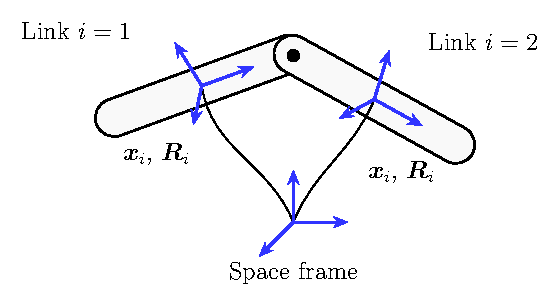
\includegraphics[width=0.65\textwidth]
        {pics/two_link_maximal_coordinates.pdf}
    \caption{Two rigid links connected by a joint in maximal coordinates.
    Adapted from \cite{BrudigamManchester2021LQR}.}
    \label{fig:maximal_coordinates_joint}
\end{figure}

A typical holonomic joint constraint can be written by equating two points
attached to different rigid bodies. This is illustrated in
Fig.~\ref{fig:maximal_coordinates_joint}. Let \(\bm{\rho}_i\) and \(\bm{\rho}_j\) denote
constant vectors from the corresponding center of mass to the joint location in
each body-fixed frame. Then a link-connecting constraint is given by
\begin{equation}
    \bm{\phi}_{ij}(q)
    =
    \bm{x}_i+\bm{R}_i\bm{\rho}_i
    -
    \bm{x}_j-\bm{R}_j\bm{\rho}_j
    =
    \bm{0}.
    \label{eq:general_joint_constraint_maximal}
\end{equation}
To include the holonomic constraints in the discrete variational principle, the
discrete action sum is augmented by Lagrange multipliers
\(\bm{\lambda}_k\in\mathbb{R}^{n_c}\). Using a trapezoidal approximation \eqref{eq:trapezodial_rule} for the
constraint contribution gives the discrete action sum
\begin{equation}
    S_{d}
    =
    \sum_{k=0}^{N-1}
    \left[
    L_d(q_k,q_{k+1})
    +
    \frac{h}{2}
    \left(
    \bm{\lambda}_k^\top \bm{\phi}(q_k)
    +
    \bm{\lambda}_{k+1}^\top \bm{\phi}(q_{k+1})
    \right)
    \right].
    \label{eq:constrained_discrete_action}
\end{equation}
%The variation with respect to \(q_k\), together with the discrete
%Lagrange--d'Alembert force contribution introduced in
%Section~\ref{sec:forced_discrete_euler_lagrange}, yields the forced and
%constrained discrete Euler-Lagrange equations
%\begin{equation}
%    D_1 L_d(q_k,q_{k+1})
%    +
%    D_2 L_d(q_{k-1},q_k)
%    +
%    \bm{u}_k
%    +
%    h\,\bm{G}(q_k)^\top \bm{\lambda}_k = 0,
%    \qquad
%    \bm{\phi}(q_k)=\bm{0},
%    \label{eq:forced_constrained_del_general}
%\end{equation}
%where
%\begin{equation}
%    \bm{G}(q_k)
%    =
%    \frac{\partial \bm{\phi}(q_k)}{\partial q_k}
%    \label{eq:constraint_jacobian_general}
%\end{equation}
%denotes the constraint Jacobian.
%Equation~\eqref{eq:forced_constrained_del_general} provides the general
%forced and constrained discrete Euler-Lagrange equation used for deriving multi-body dynamics.

\subsection{Acrobot}
\label{subsection:discrete_Acrobot}

\paragraph{Configuration Manifold}

The Acrobot model, illustrated in Fig.~\ref{fig:acrobot_maximal_coordinates},
consists of two planar rigid links connected by a revolute joint. The first link is
attached to the inertial frame by a fixed revolute joint, while the second link is
connected to the first link at the elbow. In contrast to the 3D-pendulum, the
system is described in maximal coordinates. Therefore, each link is assigned its own
center of mass position and orientation.

\begin{figure}[t]
    \centering
    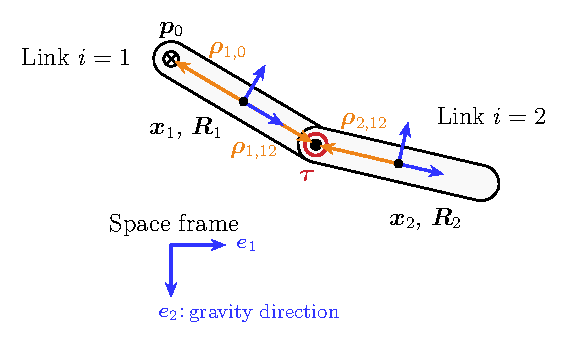
\includegraphics[width=0.75\textwidth]{pics/acrobot_maximal_coordinates.pdf}
    \caption{Acrobot configuration manifold in maximal coordinates.}
    \label{fig:acrobot_maximal_coordinates}
\end{figure}

For each link \(i\in\{1,2\}\), the center of mass position is denoted by
\(\bm{x}_i\in\mathbb{R}^2\), and the orientation of the body-fixed frame with
respect to the inertial frame is described by the rotation matrix
\(\bm{R}_i\in SO(2)\). The special orthogonal group in two dimensions is defined as
\begin{equation}
    SO(2)
    =
    \left\{
    \bm{R}\in\mathbb{R}^{2\times 2}
    \mid
    \bm{R}^{\top}\bm{R}=\bm{I}_{2},
    \ \det(\bm{R})=1
    \right\}.
    \label{eq:so2_definition}
\end{equation}
Every element \(\bm{R}_i\in SO(2)\) can be written in terms of an angle
\(\theta_i\in\mathbb{R}\) as
\begin{equation}
    \bm{R}_i
    =
    \begin{bmatrix}
        \cos\theta_i & -\sin\theta_i \\
        \sin\theta_i &  \cos\theta_i
    \end{bmatrix}.
    \label{eq:so2_rotation_matrix}
\end{equation} 
Thus, the unconstrained maximal-coordinate configuration
manifold is given by
\begin{equation}
    Q_{\mathrm{max}}
    =
    \left(
    \mathbb{R}^2 \times SO(2)
    \right)^2 .
    \label{eq:acrobot_q_max}
\end{equation}
Consequently, the constrained configuration of the Acrobot is written as
\begin{equation}
    Q_c = \{q \in Q_{\mathrm{max}} \mid \bm{\phi}(q) = \bm{0}\},
    \label{eq:acrobot_configuration}
\end{equation}
with $q = (\bm{x}_1,\bm{R}_1,\bm{x}_2,\bm{R}_2)$.
Here, \(\bm{R}_i\) maps vectors from the \(i\)-th body-fixed frame to the inertial
frame.

Let \(\bm{\rho}_{1,0}\in\mathbb{R}^2\) denote the vector from the center of mass of
link~1 to the base joint, expressed in the first body-fixed frame. Furthermore, let
\(\bm{\rho}_{1,12}\in\mathbb{R}^2\) and \(\bm{\rho}_{2,12}\in\mathbb{R}^2\) denote the
vectors from the corresponding centers of mass to the elbow joint, expressed in
the body-fixed frames of link~1 and link~2. The fixed base joint is imposed by
\begin{equation}
    \bm{\phi}_{0}(q)
    =
    \bm{x}_1
    +
    \bm{R}_1\bm{\rho}_{1,0}
    -
    \bm{p}_0
    =
    \bm{0},
    \label{eq:acrobot_base_constraint}
\end{equation}
where \(\bm{p}_0\in\mathbb{R}^2\) is the fixed base position in the inertial frame.
The elbow joint is imposed by requiring the two joint points on link~1 and link~2
to coincide, yielding
\begin{equation}
    \bm{\phi}_{12}(q)
    =
    \bm{x}_1
    +
    \bm{R}_1\bm{\rho}_{1,12}
    -
    \bm{x}_2
    -
    \bm{R}_2\bm{\rho}_{2,12}
    =
    \bm{0}.
    \label{eq:acrobot_elbow_constraint}
\end{equation}
Consequently, the full holonomic constraint vector is defined as
\begin{equation}
    \bm{\phi}(q)
    =
    \begin{bmatrix}
        \bm{\phi}_{0}(q) \\
        \bm{\phi}_{12}(q)
    \end{bmatrix}
    =
    \bm{0}.
    \label{eq:acrobot_constraints}
\end{equation}

In the discrete setting, the attitude of each link is updated by a relative rotation
\(\bm{F}_{i,k}\in SO(2)\), such that
\begin{equation}
    \bm{R}_{i,k+1}
    =
    \bm{R}_{i,k}\bm{F}_{i,k},
    \qquad i\in\{1,2\}.
    \label{eq:acrobot_rotation_update}
\end{equation}
The discrete configuration at time step \(k\) is therefore
\begin{equation}
    q_k
    =
    \left(
    \bm{x}_{1,k},\bm{R}_{1,k},
    \bm{x}_{2,k},\bm{R}_{2,k}
    \right)
    \in Q_c .
    \label{eq:acrobot_discrete_configuration}
\end{equation}

\paragraph{Continuous Lagrangian}

To derive the continuous Lagrangian of the Acrobot in maximal coordinates, the
kinetic and potential energy of both rigid links are introduced. For each link
\(i\in\{1,2\}\), the translational velocity of the center of mass is denoted by
\(\dot{\bm{x}}_i=\bm{v}_i\in\mathbb{R}^2\). Let $\bm{M}_i = m_i\bm{I}_2$ be the mass matrix of link \(i\).
The defined non-standard inertia matrix in \eqref{eq:non-standard_inertia}
is derived for $SO(3)$. In order to apply the non-standard inertia to the planar $SO(2)$ case,
the non-standard inertia matrix on \(SO(2)\) is derived by rewriting the 
planar rotational kinetic term of the discrete Lagrangian in
\cite{LeeLeokMcClamroch2007DiscreteControlSystems}. 
As a result, the relation of the non-standard
inertia to the standard inertia matrix on $SO(2)$ is given by
\begin{align}\label{eq:2D_nonstandard_inertia}
    \bm{J}_{d,i}
    =
    \frac{1}{2}J_i^{\mathrm{com}} \bm{I}_2,
\end{align}
where $J_i^{\mathrm{com}}$ is the rotational inertia of a uniform rod about its center of mass. 
The kinetic energy with its translational $T_T$ and rotational $T_R$ components is written as
\begin{equation}
    T
    =
    \underbrace{
    \sum_{i=1}^{2}
    \frac{1}{2}\bm{v}_i^{\top}\bm{M}_i\bm{v}_i
    }_{T_T}
    +
    \underbrace{
    \sum_{i=1}^{2}
    \frac{1}{2}
    \mathrm{tr}
    \left[
        \bm{\widehat{\omega}}_i
        \bm{J}_{d,i}
        \bm{\widehat{\omega}}_i^{\top}
    \right]
    }_{T_R}.
    \label{eq:acrobot_kinetic_energy_split}
\end{equation}
The gravitational potential energy is expressed directly by the center of mass
positions. In contrast to the 3D-pendulum, \cite{BrudigamManchester2021VariationalIntegrators} assumes zero potential for the rotational setting, 
which gives 
\begin{equation}
    V_R(\bm{R}_1,\bm{R}_2)=0.
    \label{eq:acrobot_rotation_potential_zero}
\end{equation}
Therefore, the gravitational potential energy is only given by the translational term
\begin{equation}
    V = V_T(\bm{x}_1,\bm{x}_2)
    =
    -
    \sum_{i=1}^{2}
    g\,\bm{e}_2^{\top}\bm{M}_i\bm{x}_i,
    \label{eq:acrobot_potential_energy}
\end{equation}
where \(\bm{e}_2\in\mathbb{R}^2\) denotes the unit vector in the gravity direction in the inertial frame.
Consequently, the continuous Lagrangian
\(L:TQ_{\mathrm{max}}\rightarrow\mathbb{R}\) is defined as
\begin{equation}
    \begin{aligned}
    L(q,\dot{q})
    &=
    \sum_{i=1}^{2}
    \left(
    \frac{1}{2}\bm{v}_i^{\top}\bm{M}_i\bm{v}_i
    +
    \frac{1}{2}
    \mathrm{tr}
    \left[
        \bm{\widehat{\omega}}_i
        \bm{J}_{d,i}
        \bm{\widehat{\omega}}_i^{\top}
    \right]
    \right)
    +
    \sum_{i=1}^{2}
    g\,\bm{e}_2^{\top}\bm{M}_i\bm{x}_i .
    \end{aligned}
    \label{eq:acrobot_continuous_lagrangian}
\end{equation}

\paragraph{Discrete Lagrangian}

In general, the discrete Lagrangian is written as
\begin{align*}
    L_d(q_k,q_{k+1})
    =
    T_{d,T}(q_k,q_{k+1})
    +
    T_{d,R}(q_k,q_{k+1})
    -
    V_{d,T}(q_k,q_{k+1}).
    \label{eq:acrobot_discrete_lagrangian_split}
\end{align*}
Following the structure of maximal-coordinate variational
integrators in \cite{BrudigamManchester2021VariationalIntegrators},
the translational and rotational parts are
discretized separately.

For the translational part, the center of mass velocity of each link is 
\begin{equation}
    \bm{v}_{i,k}
    =
    \frac{\bm{x}_{i,k+1}-\bm{x}_{i,k}}{h},
    \qquad i\in\{1,2\}.
    \label{eq:acrobot_discrete_translational_velocity}
\end{equation}
\cite{BrudigamManchester2021VariationalIntegrators} defines the discrete translational kinetic energy contribution to be
\begin{equation}
    T_{d,T}(q_k,q_{k+1})
    =
    \sum_{i=1}^{2}
    \frac{1}{2h}
    \left(
    \bm{x}_{i,k+1}-\bm{x}_{i,k}
    \right)^{\top}
    \bm{M}_i
    \left(
    \bm{x}_{i,k+1}-\bm{x}_{i,k}
    \right).
    \label{eq:acrobot_discrete_translational_lagrangian}
\end{equation}
Substituting the angular velocity approximation \eqref{eq:discrete_velocity_approximation} into the rotational kinetic energy
$T_R$ of \eqref{eq:acrobot_kinetic_energy_split}, the discrete rotational kinetic
energy contribution is derived as
\begin{equation}
\begin{aligned}
    T_{d,R}(q_k,q_{k+1})
    &=
    \sum_{i=1}^{2}
    \frac{1}{2h}
    \mathrm{tr}
    \left[
    \left(
    \bm{F}_{i,k}-\bm{I}_{2}
    \right)
    \bm{J}_{d,i}
    \left(
    \bm{F}_{i,k}-\bm{I}_{2}
    \right)^{\top}
    \right] \\
    &=
    \sum_{i=1}^{2}
    \frac{1}{h}
    \mathrm{tr}
    \left[
    \left(
    \bm{I}_{2}
    -
    \bm{F}_{i,k}
    \right)
    \bm{J}_{d,i}
    \right].
\end{aligned}
\label{eq:acrobot_discrete_rotational_lagrangian}
\end{equation}
This calculation corresponds to the discrete rotational kinetic energy of the 3D-pendulum in Section \ref{sec:discrete_3D_pendulum}.

Finally, using the trapezoidal rule for the discretization of the potential energy integral, the discrete translational potential contribution $V_{d,T}$
is given by
\begin{equation}
    V_{d,T}(q_k,q_{k+1})
    =
    -
    \frac{h}{2}
    \sum_{i=1}^{2}
    m_i g
    \bm{e}_{2}^{\top}
    \left(
    \bm{x}_{i,k}
    +
    \bm{x}_{i,k+1}
    \right).
    \label{eq:acrobot_discrete_potential_lagrangian}
\end{equation}

Combining the translational \eqref{eq:acrobot_discrete_translational_lagrangian}, rotational \eqref{eq:acrobot_discrete_rotational_lagrangian}, and potential \eqref{eq:acrobot_discrete_potential_lagrangian} contributions gives the
discrete Lagrangian
\begin{equation}
    \begin{aligned}
    L_d(q_k,q_{k+1})
    =
    &
    \text{  }
    L_d
    \left(
    \bm{x}_{1,k},\bm{x}_{1,k+1},
    \bm{x}_{2,k},\bm{x}_{2,k+1},
    \bm{F}_{1,k},\bm{F}_{2,k}
    \right)  \\
    =
    &
    \sum_{i=1}^{2}
    \frac{1}{2h}
    \left(
    \bm{x}_{i,k+1}-\bm{x}_{i,k}
    \right)^{\top}
    \bm{M}_i
    \left(
    \bm{x}_{i,k+1}-\bm{x}_{i,k}
    \right)  \\
    &
    +
    \sum_{i=1}^{2}
    \frac{1}{h}
    \mathrm{tr}
    \left[
    \left(
    \bm{I}_{2}
    -
    \bm{F}_{i,k}
    \right)
    \bm{J}_{d,i}
    \right]   \\
    &
    +
    \frac{h}{2}
    \sum_{i=1}^{2}
    g
    \bm{e}_{2}^{\top}
    \bm{M}_i
    \left(
    \bm{x}_{i,k}
    +
    \bm{x}_{i,k+1}
    \right).
    \end{aligned}
    \label{eq:acrobot_discrete_lagrangian}
\end{equation}

\paragraph{Discrete Euler-Lagrange Equations}

The discrete equations of motion are obtained from the stationary condition of the
constrained discrete action. 
The holonomic constraints introduced in
\eqref{eq:acrobot_constraints} are included by extending the action integral with
Lagrange multipliers. Let
\begin{equation}
    \bm{\lambda}
    =
    \begin{bmatrix}
        \bm{\lambda}_{0} \\
        \bm{\lambda}_{12}
    \end{bmatrix}
    \in\mathbb{R}^{4},
    \label{eq:acrobot_lagrange_multipliers}
\end{equation}
where \(\bm{\lambda}_{0}\in\mathbb{R}^2\) enforces the base constraint and
\(\bm{\lambda}_{12}\in\mathbb{R}^2\) enforces the elbow constraint.
Using the constrained action sum defined in \eqref{eq:constrained_discrete_action}, the
variation is written as
\begin{equation}
    \delta S_{d}
    =
    \delta
    \sum_{k=0}^{N-1}
    \left[
    L_d(q_k,q_{k+1})
    +
    \frac{h}{2}
    \left(
    \bm{\lambda}_{k}^{\top}\bm{\phi}(q_k)
    +
    \bm{\lambda}_{k+1}^{\top}\bm{\phi}(q_{k+1})
    \right)
    \right]
    = 0.
    \label{eq:acrobot_variation_constrained_discrete_action}
\end{equation}
The translational and rotational components are treated separately, following the
maximal-coordinate variational-integrator structure. In \cite{BrudigamManchester2021VariationalIntegrators},
the variation of the translational component is given as
\begin{equation}
    \delta_{\bm{x}_{i,k+1}} S_{d,c}
    =
    \left\langle
    \left(\frac{1}{h}\bm{M}_i
    \left(
    \bm{v}_{i,k}
    -
    \bm{v}_{i,k+1}
    \right)
    +
    g\bm{M}_i\bm{e}_2
    +
    \bm{G}_{x_i,k+1}^{\top}\bm{\lambda}_{k+1}\right) h,
    \delta\bm{x}_{i,k+1}
    \right\rangle,
    \label{eq:acrobot_translational_variation}
\end{equation}
using the relation \eqref{eq:acrobot_discrete_translational_velocity}. $\bm{G}_{x_i,k+1}$ is defined as the Jacobian of the constraints $\bm{\phi}(q_{k+1})$ with respect to $\bm{x}_{i,k+1}$.
The constraint contribution is calculated as
\begin{equation}
    \bm{G}_{x,k+1}^{\top}\bm{\lambda}_{k+1}
    =
    \begin{bmatrix}
        \dfrac{\partial \bm{\phi}_{0,k+1}}{\partial \bm{x}_{1,k+1}}
        &
        \dfrac{\partial \bm{\phi}_{0,k+1}}{\partial \bm{x}_{2,k+1}}
        \\[0.8em]
        \dfrac{\partial \bm{\phi}_{12,k+1}}{\partial \bm{x}_{1,k+1}}
        &
        \dfrac{\partial \bm{\phi}_{12,k+1}}{\partial \bm{x}_{2,k+1}}
    \end{bmatrix}^{\top}
    \begin{bmatrix}
        \bm{\lambda}_{0,k+1} \\
        \bm{\lambda}_{12,k+1}
    \end{bmatrix}  
    =
    \begin{bmatrix}
        \bm{\lambda}_{0,k+1}+\bm{\lambda}_{12,k+1} \\
        -\bm{\lambda}_{12,k+1}
    \end{bmatrix}.
    \label{eq:acrobot_translational_constraint_force}
\end{equation}
with the discretized constraints
\begin{equation}
    \bm{\phi}(q_{k+1})
    =
    \begin{bmatrix}
        \bm{\phi}_{0,k+1} \\
        \bm{\phi}_{12,k+1}
    \end{bmatrix}
    =
    \begin{bmatrix}
    \bm{x}_{1,k+1}
    +
    \bm{R}_{1,k+1}\bm{\rho}_{1,0}
    -
    \bm{p}_0
    \\
    \bm{x}_{1,k+1}
    +
    \bm{R}_{1,k+1}\bm{\rho}_{1,12}
    -
    \bm{x}_{2,k+1}
    -
    \bm{R}_{2,k+1}\bm{\rho}_{2,12}
    \end{bmatrix}.
    \label{eq:acrobot_discrete_constraints_vector}
\end{equation}
Therefore, substituting the gradient \eqref{eq:acrobot_translational_constraint_force} into \eqref{eq:acrobot_translational_variation}, the translational discrete Euler-Lagrange equations for link 1 and link 2 are
\begin{subequations}
\label{eq:acrobot_translational_del_links}
\begin{align}
    \frac{1}{h}\bm{M}_{1}
    \left(
    \bm{v}_{1,k+1}
    -
    \bm{v}_{1,k}
    \right)
    -
    g\bm{M}_{1}\bm{e}_{2}
    -
    \left(
    \bm{\lambda}_{0,k+1}
    +
    \bm{\lambda}_{12,k+1}
    \right)
    &=
    \bm{0},
    \label{eq:acrobot_translational_del_link_1}
    \\
    \frac{1}{h}\bm{M}_{2}
    \left(
    \bm{v}_{2,k+1}
    -
    \bm{v}_{2,k}
    \right)
    -
    g\bm{M}_{2}\bm{e}_{2}
    +
    \bm{\lambda}_{12,k+1}
    &=
    \bm{0}.
    \label{eq:acrobot_translational_del_link_2}
\end{align}
\end{subequations}

For the rotational part, the derivatives of \eqref{eq:discrete_euler_lagrange_lie_group} have to be taken for each link, analogously to the 3D-pendulum of Section \ref{sec:discrete_3D_pendulum}.
Firstly, the directional derivative $\left\langle D_{\bm{F}_{i,k}}L_d(\bm{F}_{i,k}), \delta \bm{F}_{i,k} \right\rangle$ is given by applying Proposition \eqref{prop:directional_derivative_discrete_f}, which yields
\begin{equation}
    \begin{aligned}
    \left\langle
    T_e^*\mathbb{L}_{\bm{F}_{i,k}}
    D_{\bm{F}_{i,k}}L_{d,R,i},
    \widehat{\bm{X}}_k
    \right\rangle
    &=
    \left.
    \frac{d}{d\epsilon}
    \right|_{\epsilon=0}
    L_{d}
    \left(
    \bm{F}_{i,k}
    \exp(\epsilon\widehat{\bm{X}}_k)
    \right)
    \\
    &=
    -
    \frac{1}{h}
    \mathrm{tr}
    \left[
    \bm{F}_{i,k}
    \widehat{\bm{X}}_k
    \bm{J}_{d,i}
    \right]
    \\
    &=
    \left\langle
    \frac{1}{h}
    \left(
    \bm{J}_{d,i}\bm{F}_{i,k}
    -
    \bm{F}_{i,k}^{\top}\bm{J}_{d,i}
    \right),
    \widehat{\bm{X}}_k
    \right\rangle
    \\
    &=
    \left\langle
    \bm{\widehat{\Pi}}_{i,k}
    ,
    \widehat{\bm{X}}_k
    \right\rangle
    , 
    \end{aligned}
    \label{eq:acrobot_rotational_derivative_pairing}
\end{equation}
corresponding to the derivative of the single body 3D-pendulum derived in Section \ref{sec:discrete_3D_pendulum}. 
Here,
\begin{equation}
    \bm{\widehat{\Pi}}_{i,k}
    =
    \frac{1}{h}
    \left(
        \bm{J}_{d,i}\bm{F}_{i,k}
        -
        \bm{F}_{i,k}^{\top}\bm{J}_{d,i}
    \right),
    \qquad i\in\{1,2\},
    \label{eq:acrobot_discrete_angular_momentum}
\end{equation}
denotes the discrete angular momentum
of link \(i\) associated with the relative rotation \(\bm{F}_{i,k}\).
It is the analogue of the discrete Legendre momentum \eqref{eq:discrete_3D_pendulum_momentum_1} used for
the 3D-pendulum in Section \ref{sec:discrete_3D_pendulum}, now defined separately for each rigid link \cite{Lee2008}.

Since \(SO(2)\) is abelian, it follows that \(\operatorname{Ad}_{\bm{F}_{i,k}}=\bm{I}\) \cite{Lee2008}.
Therefore, the coadjoint term is equal to \eqref{eq:acrobot_rotational_derivative_pairing} at time step $k+1$, which gives
\begin{equation}\label{eq:acrobot_Ad_variation}
\operatorname{Ad}^{*}_{\bm{F}_{i,k+1}^{-1}}
\!\left(
T_e^*\mathbb{L}_{\bm{F}_{i,k+1}}
D_{\bm{F}_{i,k+1}}L_d(\bm{F}_{i,k+1})
\right)
= 
\frac{1}{h}
\left(
\bm{J}_{d,i}\bm{F}_{i,k+1}
-
\bm{F}_{i,k+1}^{\top}\bm{J}_{d,i}
\right).
\end{equation}
It remains to derive the directional derivative of the rotations $\bm{R}_{i,k+1}$. 
From \eqref{eq:acrobot_variation_constrained_discrete_action}, it is observed that only the constraints $\bm{\phi}(q_k)$ are dependent on
the rotation matrices \(\bm{R}_{1,k}\) and \(\bm{R}_{2,k}\). 
Hence, the variation of the constraint contribution 
\begin{equation*}
    \left\langle D_{\bm{R}_{i,k+1}}(h \bm{\lambda}_{k+1}^\top \bm{\phi}_{k+1}), \delta \bm{R}_{i,k+1} \right\rangle=\left\langle T_e^* \mathbb{L}_{\bm{R}_{i,k+1}} D_{\bm{R}_{i,k+1}}(h \bm{\lambda}_{k+1}^\top \bm{\phi}_{k+1}), \bm{\widehat{\eta}}_{i,k+1} \right\rangle,
\end{equation*}
has to be evaluated for each link $i$, using Proposition \eqref{prop:directional_derivative_discrete_g}. For link $i=1$, the variation of the constraint contribution is given by
\begin{equation}
    \begin{aligned}
    &
    \left\langle
    T_e^*\mathbb{L}_{\bm{R}_{1,k+1}}
    D_{\bm{R}_{1,k+1}}
    \left(
    h\bm{\lambda}_{k+1}^{\top}\bm{\phi}_{k+1}
    \right),
    \bm{\widehat{\eta}}_{1,k+1}
    \right\rangle
    \\
    &=
    \left.
    \frac{d}{d\epsilon}
    \right|_{\epsilon=0}
    h
    \left[
    \bm{\lambda}_{0,k+1}^{\top}
    \bm{\phi}_{0,k+1}^{\epsilon}
    +
    \bm{\lambda}_{12,k+1}^{\top}
    \bm{\phi}_{12,k+1}^{\epsilon}
    \right]
    \\
    &=
    h 
    \left[
    \bm{\lambda}_{0,k+1}^{\top}
    \bm{R}_{1,k+1}\bm{\widehat{\eta}}_{1,k+1}\bm{\rho}_{1,0}
    +
    \bm{\lambda}_{12,k+1}^{\top}
    \bm{R}_{1,k+1}\bm{\widehat{\eta}}_{1,k+1}\bm{\rho}_{1,12}
    \right]
    \\
    &=
    h
    \left[
    \left(
    \bm{\rho}_{1,0}
    \times
    \bm{R}_{1,k+1}^{\top}\bm{\lambda}_{0,k+1}
    \right)
    +
    \left(
    \bm{\rho}_{1,12}
    \times
    \bm{R}_{1,k+1}^{\top}\bm{\lambda}_{12,k+1}
    \right)
    \right]
    \cdot
    \eta_{1,k+1}
    \\
    &=
    \left\langle
    h
    \left[
    \left(
    \bm{\rho}_{1,0}
    \times
    \bm{R}_{1,k+1}^{\top}\bm{\lambda}_{0,k+1}
    \right)
    +
    \left(
    \bm{\rho}_{1,12}
    \times
    \bm{R}_{1,k+1}^{\top}\bm{\lambda}_{12,k+1}
    \right)
    \right]^{\wedge},
    \bm{\widehat{\eta}}_{1,k+1}
    \right\rangle,
    \end{aligned}
    \label{eq:acrobot_R1_constraint_derivative_kp1}
\end{equation}
whose calculation corresponds to the derivative of the 3D-pendulum with respect to the rotation matrix $\bm{R}_k$ derived in Section \ref{sec:discrete_3D_pendulum}.
Here, the planar cross product of $\boldsymbol{a},\boldsymbol{b}\in\mathbb{R}^{2}$ is defined as
$\boldsymbol{a}^{\top}\widehat{\eta}\,\boldsymbol{b}=(\boldsymbol{b}\times\boldsymbol{a}) \cdot \eta$, using the $SO(2)$ hat map \eqref{eq:hat_map_so2}.
In contrast, the variation of the constraint contribution for link $i=2$ only depends on $\bm{\phi}_{12,k+1}$ and is derived as
\begin{equation}
    \begin{aligned}
    &
    \left\langle
    T_e^*\mathbb{L}_{\bm{R}_{2,k+1}}
    D_{\bm{R}_{2,k+1}}
    \left(
    h\bm{\lambda}_{k+1}^{\top}\bm{\phi}_{k+1}
    \right),
    \bm{\widehat{\eta}}_{2,k+1}
    \right\rangle
    \\
    &=
    \left.
    \frac{d}{d\epsilon}
    \right|_{\epsilon=0}
    h
    \left[
    \bm{\lambda}_{12,k+1}^{\top}
    \bm{\phi}_{12,k+1}^{\epsilon}
    \right]
    \\
    &=
    \left.
    \frac{d}{d\epsilon}
    \right|_{\epsilon=0}
    h
    \left[
    \bm{\lambda}_{12,k+1}^{\top}
    \left(
    -
    \bm{R}_{2,k+1}
    \exp(\epsilon\bm{\widehat{\eta}}_{2,k+1})
    \bm{\rho}_{2,12}
    \right)
    \right]
    \\
    &=
    -h
    \left[
    \bm{\lambda}_{12,k+1}^{\top}
    \bm{R}_{2,k+1}
    \bm{\widehat{\eta}}_{2,k+1}
    \bm{\rho}_{2,12}
    \right]
    \\
    &=
    -h
    \left(
    \bm{\rho}_{2,12}
    \times
    \bm{R}_{2,k+1}^{\top}\bm{\lambda}_{12,k+1}
    \right)
    \cdot
    \eta_{2,k+1}
    \\
    &=
    \left\langle
    -h
    \left(
    \bm{\rho}_{2,12}
    \times
    \bm{R}_{2,k+1}^{\top}\bm{\lambda}_{12,k+1}
    \right)^{\wedge},
    \bm{\widehat{\eta}}_{2,k+1}
    \right\rangle .
    \end{aligned}
    \label{eq:acrobot_R2_constraint_derivative_kp1}
\end{equation}

The full rotational contribution is described by substituting \eqref{eq:acrobot_rotational_derivative_pairing}, \eqref{eq:acrobot_Ad_variation}, \eqref{eq:acrobot_R1_constraint_derivative_kp1} and \eqref{eq:acrobot_R2_constraint_derivative_kp1} for each link $i = 1,2$ into \eqref{eq:discrete_euler_lagrange_lie_group}. Moreover, \eqref{eq:acrobot_translational_del_links} gives the translational description.
Finally, the full discrete Euler-Lagrange equations of the unforced Acrobot in maximal coordinates are expressed on \(\left(\mathbb{R}^2\times SO(2)\right)^2\) as
\begin{subequations}
\label{eq:acrobot_full_del_shifted}
\begingroup
\small
\setlength{\jot}{0.35em}
\vspace{-0.3cm}
\begin{align}
    \intertext{\textit{Translation:}}
    \vspace{-0.1cm}
    \frac{1}{h}\bm{M}_{1}
    \left(
        \bm{v}_{1,k+1}
        -
        \bm{v}_{1,k}
    \right)
    -
    g\bm{M}_{1}\bm{e}_2
    -
    \left(
        \bm{\lambda}_{0,k+1}
        +
        \bm{\lambda}_{12,k+1}
    \right)
    &=
    \bm{0},
    \label{eq:acrobot_full_del_shifted_translation_1}
    \\
\hspace{-2em}
    \frac{1}{h}\bm{M}_{2}
    \left(
        \bm{v}_{2,k+1}
        -
        \bm{v}_{2,k}
    \right)
    -
    g\bm{M}_{2}\bm{e}_2
    +
    \bm{\lambda}_{12,k+1}
    &=
    \bm{0},
    \label{eq:acrobot_full_del_shifted_translation_2}
\end{align}
\vspace{-0.4cm}
\vspace{-0.6cm}
\begin{align}
    \intertext{\textit{Rotation:}}
    \vspace{-0.1cm}
    \bm{\widehat{\Pi}}_{1,k}
    -
    \bm{\widehat{\Pi}}_{1,k+1}
    +
    h
    \left[
    \left(
    \bm{\rho}_{1,0}
    \times
    \bm{R}_{1,k+1}^{\top}\bm{\lambda}_{0,k+1}
    \right)
    +
    \left(
    \bm{\rho}_{1,12}
    \times
    \bm{R}_{1,k+1}^{\top}\bm{\lambda}_{12,k+1}
    \right)
    \right]^{\wedge}
    &=
    \bm{0},
    \label{eq:acrobot_full_del_shifted_rotation_1}
    \\
\hspace{-2em}
    \bm{\widehat{\Pi}}_{2,k}
    -
    \bm{\widehat{\Pi}}_{2,k+1}
    -
    h
    \left[
    \left(
    \bm{\rho}_{2,12}
    \times
    \bm{R}_{2,k+1}^{\top}\bm{\lambda}_{12,k+1}
    \right)
    \right]^{\wedge}
    &=
    \bm{0},
    \label{eq:acrobot_full_del_shifted_rotation_2}
\end{align}
\vspace{-0.4cm}
\vspace{-0.6cm}
\begin{align}
    \intertext{\textit{Constraints:}}    
    \bm{\phi}_{0,k+1}
    =
    \bm{x}_{1,k+1}
    +
    \bm{R}_{1,k+1}\bm{\rho}_{1,0}
    -
    \bm{p}_0
    &=
    \bm{0},
    \label{eq:acrobot_full_del_shifted_base_constraint}
    \\
\hspace{-2em}
    \bm{\phi}_{12,k+1}
    =
    \bm{x}_{1,k+1}
    +
    \bm{R}_{1,k+1}\bm{\rho}_{1,12}
    -
    \bm{x}_{2,k+1}
    -
    \bm{R}_{2,k+1}\bm{\rho}_{2,12}
    &=
    \bm{0},
    \label{eq:acrobot_full_del_shifted_elbow_constraint}
\end{align}
\vspace{-0.4cm}    
\vspace{-0.6cm}
\begin{align}
    \intertext{\textit{Kinematics:}}    
    \bm{R}_{1,k+1}
    &=
    \bm{R}_{1,k}\bm{F}_{1,k},
    \label{eq:acrobot_full_del_shifted_kinematics_1}
    \\
\hspace{-2em}
    \bm{R}_{2,k+1}
    &=
    \bm{R}_{2,k}\bm{F}_{2,k}.
    \label{eq:acrobot_full_del_shifted_kinematics_2}
\end{align}
\endgroup
\end{subequations}
subject to the constraints \eqref{eq:acrobot_constraints}.

\paragraph{Controlled Acrobot}

As in the controlled 3D-pendulum case of Section \ref{sec:discrete_3D_pendulum}, the trapezoidal approximation distributes
the virtual work equally to both endpoints of the interval \eqref{eq:generalized_forced_3D_pendulum}. Therefore, the discrete
Legendre force contributions of \eqref{eq:discrete_forces_special} are given by 
\begin{align}
    \bm{\tau}^-_{d,k}= \frac{h}{2}\bm{\tau}_{k}, \quad \bm{\tau}^+_{d,k}= \frac{h}{2}\bm{\tau}_{k+1},
    \label{eq:acrobot_force_contribution}
\end{align}
The Acrobot is actuated by a single motor located at the elbow joint \cite{BrudigamManchester2021LQR}. In contrast
to the controlled 3D-pendulum, the input is therefore not an external moment acting
on one rigid body, but an internal joint torque acting between the two links. The generalized torque vector
is defined as
\begin{equation}
    \bm{\tau}_k
    =
    \begin{bmatrix}
        -u_k \\
         u_k
    \end{bmatrix},
    \label{eq:acrobot_generalized_torque}
\end{equation}
where \(u_k\in\mathbb{R}\) is the scalar elbow torque that applies 
opposite moments between the two links.

Since the Acrobot is actuated by a motor at the elbow joint, the control input is a
pure rotational torque acting between the two links. Hence, there is no external
translational force acting directly on the centers of mass, and the translational
force contribution is set to
\begin{equation}
    \bm{u}^{x}_{1,k}
    =
    \bm{u}^{x}_{2,k}
    =
    \bm{0}.
    \label{eq:acrobot_zero_translational_force}
\end{equation}
Using the discrete Lagrange-d'Alembert principle \eqref{eq:discrete_forced_Euler_Lagrange}, the generalized torque
contribution \eqref{eq:acrobot_force_contribution} under the definition of torque vector $\bm{\tau}_k$ \eqref{eq:acrobot_generalized_torque} is added only to the unforced 
rotational equations \eqref{eq:acrobot_full_del_shifted_rotation_1} and \eqref{eq:acrobot_full_del_shifted_rotation_2}. 
In consequence, the controlled rotational discrete Euler-Lagrange equations are derived as
\begin{subequations}
\label{eq:forced_acrobot_rotational_equations}
\begingroup
\footnotesize
\setlength{\jot}{0.25em}
\begin{align}
    \bm{\widehat{\Pi}}_{1,k}
    -
    \bm{\widehat{\Pi}}_{1,k+1}
    +
    h
    \left[
    \left(
    \bm{\rho}_{1,0}
    \times
    \bm{R}_{1,k+1}^{\top}\bm{\lambda}_{0,k+1}
    \right)
    +
    \left(
    \bm{\rho}_{1,12}
    \times
    \bm{R}_{1,k+1}^{\top}\bm{\lambda}_{12,k+1}
    \right)
    -
    u_{k+1}
    \right]^{\wedge}
    &=
    \bm{0},
    \label{eq:forced_acrobot_rotation_link1}
    \\
    \bm{\widehat{\Pi}}_{2,k}
    -
    \bm{\widehat{\Pi}}_{2,k+1}
    +
    h
    \left[
    u_{k+1}
    -
    \left(
    \bm{\rho}_{2,12}
    \times
    \bm{R}_{2,k+1}^{\top}\bm{\lambda}_{12,k+1}
    \right)
    \right]^{\wedge}
    &=
    \bm{0}.
    \label{eq:forced_acrobot_rotation_link2}
\end{align}
\endgroup
\end{subequations}
For \(u_{k+1}=0\), these equations reduce to the corresponding unforced rotational
equations derived previously.
\chapter{Certifiable Trajectory Optimization via Semidefinite Relaxation}
\label{chapter:certifiable_trajectory_optimization}

This chapter formulates the discrete rigid-body models derived in 
Chapter \ref{chapter:discrete_mechanics_for_rigid_bodies_on_lie_groups} as 
finite-horizon trajectory optimization problems. Section \ref{sec:discrete_motion_planning_of_rigid_body_systems} 
introduces the geometric motion planning 
formulation of \cite{Sangli2025}, which expresses the Lie group variational 
integrators and their kinematic constraints by polynomial equalities and inequalities. 
In general, a nonconvex polynomial optimization problem is relaxed to a convex semidefinite 
program. Therefore, Section \ref{sec:semidefinite_optimization_relaxation} gives an 
overall introduction to semidefinite programming and presents the 
Moment-SOS hierarchy and the exploitation of correlative and term sparsity. 
Finally, Sections \ref{sec:discrete_motion_planning_3d_pendulum} and 
\ref{sec:discrete_motion_planning_acrobot} define the optimization formulation for 
the controlled 3D-pendulum and the Acrobot. The resulting construction follows the sparse 
semidefinite trajectory optimization framework SPOT of \cite{Kang_2026Fast,Kang_2025Global}.
For the Acrobot, the sparse SDP relaxation is embedded in a model predictive control loop. 
Because the prediction-horizon relaxation is not rank one, the extracted predicted trajectory 
is not certified as globally optimal or feasible. Nevertheless, applying the first extracted 
control and simulating the controlled LGVI produces a 
dynamically consistent numerical closed-loop trajectory.

\section{Discrete Motion Planning of Rigid-Body Systems}
\label{sec:discrete_motion_planning_of_rigid_body_systems}

A general robot motion planning problem is modeled as a mechanical system 
consisting of \(n_{\mathrm b}\) rigid links, 
indexed by \(i\in\mathcal B:=\{1,\ldots,n_{\mathrm b}\}\), with $N$ steps starting at $k=0$. 
The robot configuration state \(\bm{Y}_k\) consists of the center-of-mass positions \(\bm{x}_{i,k}\), 
rotations \(\bm{R}_{i,k}\). The relative rotations \(\bm{F}_{i,k}\) are recunstructed from the 
kinematic update \eqref{eq:discrete_lie_group_kinematics}. The control input is denoted 
by \(\bm{U}_{k+1}\), with \(\bm{\lambda}_{k+1}\) being the Lagrange multipliers of the holonomic joint 
constraints. Adapted from the discrete kinodynamic motion planning problem of 
\cite{Sangli2025}, the general multi-body problem is written as
\begin{subequations}
\label{eq:general_motion_optimization}
\begin{align}
\min_{\{\bm{Y}_k\}_{k=0}^{N},\{\bm{U}_k,\bm{\lambda}_k\}_{k=1}^{N}}
&\quad \Psi(\bm{Y}_N)+\sum_{k=0}^{N-1}\psi(\bm{Y}_k,\bm{U}_{k+1},\bm{\lambda}_{k+1})\\
\text{s.t.}\quad
&\mathcal D_i(\bm{Y}_{k+1},\bm{Y}_k,\bm{U}_{k+1},\bm{\lambda}_{k+1})=0, \qquad i\in\mathcal B,\\
&\bm{Y}_k\in\mathcal Y_i, \\
&\mathcal{H}(\bm{Y}_{k+1},\bm{U}_{k+1},\bm{\lambda}_{k+1})\geq0,\\
&\bm{U}_{\min}\leq \bm{U}_{k+1}\leq \bm{U}_{\max},\\
&\bm{Y}_0=\bm{Y}_{\mathrm{init}},\\
&k=0,\ldots,N-1. \nonumber
\end{align}
\end{subequations}
Here, \(\Psi(\cdot)\) denotes the terminal costs and \(\psi(\cdot)\) the running costs. 
The equality constraint set \(\mathcal D_i=0\) represents the forced 
discrete Euler--Lagrange equations of link \(i\) derived in Chapter \ref{chapter:discrete_mechanics_for_rigid_bodies_on_lie_groups}, 
including the set of control inputs $\bm{U}_{k+1}$ and Lagrange multipliers $\bm{\lambda}_{k+1}$. Additionally,
for multi-body systems, the set
\(\mathcal D_i\) contains the holonomic joint constraints \eqref{eq:holonomic_constraints_general}.
The inequalities \(\mathcal{H}\geq0\) describe rotation-step limits, 
geometric constraints such as collision avoidance, and bounds introduced to obtain a compact feasible set \cite{Kang_2026Fast}. 
Control limits are set by \(\bm{U}_{\min}\leq \bm{U}_k\leq \bm{U}_{\max}\) in \eqref{eq:general_motion_optimization}.

The set \(\mathcal Y_i\) enforces the matrix Lie-group structure of the set of states $\bm{Y}_k$. 
Thereby, the multiplicative kinematic update 
\begin{equation}
\bm{R}_{i,k+1}=\bm{R}_{i,k}\bm{F}_{i,k}
\label{eq:general_lie_group_kinematics}
\end{equation}
preserves the corresponding Lie group structure for each link \(i\). 

For rigid-body motion on $SO(3)$, 
the rotation of link \(i\) is given by
\[
\bm{R}_{i,k}=
\begin{bmatrix}
\bm{r}^{1}_{i,k},&\bm{r}^{2}_{i,k},&\bm{r}^{3}_{i,k}
\end{bmatrix}
\in\mathbb R^{3\times3}.
\]
Following \cite{Sangli2025}, 
$\bm{R}_{i,k} \in \mathrm{SO}(3)$ is represented by the 
15 quadratic polynomial equalities
\begin{align}
&\|\bm{r}^{1}_{i,k}\|_2^2-1
=
\|\bm{r}^{2}_{i,k}\|_2^2-1
=
\|\bm{r}^{3}_{i,k}\|_2^2-1
=0,\nonumber\\
&(\bm{r}^{1}_{i,k})^\top \bm{r}^{2}_{i,k}
=
(\bm{r}^{2}_{i,k})^\top \bm{r}^{3}_{i,k}
=
(\bm{r}^{1}_{i,k})^\top \bm{r}^{3}_{i,k}
=0,
\label{eq:so3_polynomial_constraints}\\
&\bm{r}^{1}_{i,k}\times \bm{r}^{2}_{i,k}-\bm{r}^{3}_{i,k}
=
\bm{r}^{2}_{i,k}\times \bm{r}^{3}_{i,k}-\bm{r}^{1}_{i,k}
=
\bm{r}^{3}_{i,k}\times \bm{r}^{1}_{i,k}-\bm{r}^{2}_{i,k}
=\bm{0}_{3\times1}.
\nonumber
\end{align}
The same constraints are imposed on \(\bm{F}_{i,k}\) by replacing
\(\bm{r}^{1}_{i,k},\bm{r}^{2}_{i,k},\bm{r}^{3}_{i,k}\) with its columns
\(\bm{f}^{1}_{i,k},\bm{f}^{2}_{i,k},\bm{f}^{3}_{i,k}\).

For rigid-body motion on $SO(2)$, the standard polynomial parametrization is
\begin{equation}
\bm{R}_{i,k}=
\begin{bmatrix}
c_{i,k}&-s_{i,k}\\
s_{i,k}&c_{i,k}
\end{bmatrix},
\qquad
\bm{F}_{i,k}=
\begin{bmatrix}
a_{i,k}&-b_{i,k}\\
b_{i,k}&a_{i,k}
\end{bmatrix},
\end{equation}
where \(c_{i,k}=\cos\theta_{i,k}\), \(s_{i,k}=\sin\theta_{i,k}\), \(a_{i,k}=\cos\Delta\theta_{i,k}\), and \(b_{i,k}=\sin\Delta\theta_{i,k}\) \cite{Hall2000LieGroups}. 
Applying \eqref{eq:so2_polynomial_constraints} 
to the kinematic update for each link \(i\) in \eqref{eq:general_lie_group_kinematics},
its planar version is given by
\begin{align}
c_{i,k+1}-c_{i,k}a_{i,k}+s_{i,k}b_{i,k}=0,
\qquad
s_{i,k+1}-s_{i,k}a_{i,k}-c_{i,k}b_{i,k}=0,
\end{align}
for planar motion. In contrast to \eqref{eq:so3_polynomial_constraints}, the planar rotation matrices
\(\bm{R}_{i,k},\bm{F}_{i,k} \in \mathrm{SO}(2)\) are imposed by the two quadratic polynomial equalities
\begin{align}\label{eq:so2_polynomial_constraints}
c_{i,k}^2+s_{i,k}^2=1,
\qquad
a_{i,k}^2+b_{i,k}^2=1, 
\end{align}
\cite{Sangli2025}.

The matrix in \eqref{eq:so2_polynomial_constraints} describes a rotation in the \(xy\)-plane and therefore about the \(z\)-axis. In general, rotations about a fixed axis are
\begin{equation}
\bm{R}_x=
\begin{bmatrix}
1&0&0\\
0&c&-s\\
0&s&c
\end{bmatrix},
\qquad
\bm{R}_y=
\begin{bmatrix}
c&0&s\\
0&1&0\\
-s&0&c
\end{bmatrix},
\qquad
\bm{R}_z=
\begin{bmatrix}
c&-s&0\\
s&c&0\\
0&0&1
\end{bmatrix},
\label{eq:axis_rotations}
\end{equation}
with \(c=\cos\theta\) and \(s=\sin\theta\) \cite{Sangli2025}.
Consequently, planar motion in the \(yz\)-, \(xz\)-, or \(xy\)-plane corresponds to a rotation about the \(x\)-, \(y\)-, or \(z\)-axis.

Finally, from a given initial configuration $\bm{Y}_k$, the target configuration $\bm{Y}_N$ is reached by minimizing the terminal cost \(\Psi(\cdot)\).

\section{Semidefinite Optimization and Relaxation}
\label{sec:semidefinite_optimization_relaxation}

The discrete motion planning problem \eqref{eq:general_motion_optimization} is considered as a 
polynomial optimization problem (POP) 
with polynomial objective, equality, and inequality constraints \cite{Sangli2025}. Thereby,
\(\bm{z}\in\mathbb{R}^{n_z}\) is the complete set of states $\bm{Y}_k$, control
inputs $\bm{U}_k$, and Lagrange multipliers $\bm{\lambda}_{k+1}$ over the planning horizon. 
Equivalently, the POP can be written in the general form
\begin{subequations}\label{eq:pop_general}
\begin{align}
 p^\star = \min_{\bm{z}\in\mathbb{R}^{n_z}}
 &\quad p(\bm{z})
 \label{eq:pop_general_objective}\\
 \text{s.t.}\quad
 &h_l(\bm{z})=0, &&l=1,\ldots,m_h,
 \label{eq:pop_general_equalities}\\
 &g_j(\bm{z})\geq 0, &&j=1,\ldots,m_g,
 \label{eq:pop_general_inequalities}
\end{align}
\end{subequations}
with the basic closed semialgebraic feasible set
\begin{equation}
 \mathcal{K}:=
 \left\{\bm{z}\in\mathbb{R}^{n_z}\ \middle|\
 h_l(\bm{z})=0,\ l=1,\ldots,m_h,\;
 g_j(\bm{z})\geq0,\ j=1,\ldots,m_g\right\}.
 \label{eq:pop_feasible_set}
\end{equation}
Here, \(p\), \(h_l\), and \(g_j\) are real multivariate polynomials. In general,
a multivariate polynomial is defined as
\begin{equation}
 p(\bm{z})=\sum_{\bm{\alpha}}p_{\bm{\alpha}}\bm{z}^{\bm{\alpha}},
 \qquad
 \bm{z}^{\bm{\alpha}}:=\prod_{i=1}^{n_z}z_i^{\alpha_i},
 \label{eq:multivariate_polynomial}
\end{equation} 
where $\alpha_i$ are nonnegative integers and \(p_{\bm{\alpha}}\) are nonzero \cite{Yang2024Semidefinite}.
Although \eqref{eq:pop_general} is generally nonconvex, the Moment--SOS hierarchy constructs a
sequence of convex semidefinite relaxations whose optimal values are certified
lower bounds on the optimal solution \(p^\star\) \cite{Yang2024Semidefinite}.

\subsection{Semidefinite Relaxation and the Moment-SOS Hierarchy}
\label{subsec:moment_sos_hierarchy}

\paragraph{Semidefinite programming (SDP)}
Let \(\mathbb{S}^{n}\) denote the vector space of symmetric \(n\times n\)
matrices. A matrix \(\bm{X}\in\mathbb{S}^{n}\) is positive semidefinite,
written as \(\bm{X}\succeq0\), if
\(\bm{v}^{\top}\bm{X}\bm{v}\geq0\) for all
\(\bm{v}\in\mathbb{R}^{n}\). A semidefinite program (SDP) has the standard
primal form
\begin{equation}
\begin{aligned}
 p_{\mathrm{SDP}}^\star
 =\min_{\bm{X}\in\mathbb{S}^{n}}
 &\quad \left\langle\bm{C},\bm{X}\right\rangle\\
 \text{s.t.}\quad
 &\mathcal{A}(\bm{X})=\bm{b},\\
 &\bm{X}\succeq0.
\end{aligned}
\label{eq:standard_sdp}
\end{equation}
where $\bm{C} \in \mathbb{S}^{n}$ and $\bm{b} \in \mathbb{R}^{m}$. The linear map \(\mathcal{A}: \mathbb{S}^{n} \to \mathbb{R}^{m}\) is defined as
\begin{equation}
 \mathcal{A}(\bm{X})
 :=
 \begin{bmatrix}
 \langle\bm{A}_1,\bm{X}\rangle\\
 \vdots\\
 \langle\bm{A}_i,\bm{X}\rangle\\
 \langle\bm{A}_m,\bm{X}\rangle
 \end{bmatrix}.
 \label{eq:linear_map}
\end{equation}
Here, \(\langle\bm{C},\bm{X}\rangle=
\operatorname{tr}(\bm{C}\bm{X})\). 
In contrast to \eqref{eq:pop_general}, the objective and the
constraints in \eqref{eq:standard_sdp} are convex. In the following, the Moment-SOS 
relaxation approximates the nonconvex polynomial problem by a convex SDP \cite{Yang2024Semidefinite}.

\paragraph{Sum-of-squares (SOS) relaxation}
\cite{Yang2024Semidefinite} defines a monomial
of the optimization variables \(\bm{z}=(z_1,\ldots,z_{n_z})\) as
\begin{equation}
\bm{z}^{\bm{\alpha}}:=\prod_{i=1}^{n_z}z_i^{\alpha_i},
\label{eq:monomial_basis_comparison}
\end{equation}
with \(\bm{\alpha}=(\alpha_1,\ldots,\alpha_{n_z})\in\mathbb{N}_0^{n_z}\). Thereby, 
$|\bm{\alpha}|:=\sum_{i=1}^{n_z}\alpha_i$ is the total degree of the monomial $\bm{z}^{\bm{\alpha}}$. 
Moreover, the standard basis of monomials with
degree up to \( |\bm{\alpha}|\leq d\) is given by
\[
[\bm{z}]_d:=
\begin{bmatrix}
1 & z_1 & \cdots & z_{n_z} & z_1^2 & z_1z_2 & \cdots & z_{n_z}^d
\end{bmatrix}^{\top}
=
\left[\bm{z}^{\bm{\alpha}}\right]_{\bm{\alpha}\in\mathbb{N}_0^{n_z}},
\]
The vector has dimension
\begin{equation}
s(n_z,d)=\binom{n_z+d}{d}.
\label{eq:monomial_basis_dimension_comparison}
\end{equation}
\cite{Yang2024Semidefinite} defines a polynomial \(p\) of degree at most \(2d\) as a sum of squares (SOS)
if it can be written as
\(p(\bm{z})=\sum_i q_i(\bm{z})^2\). Here, each \(q_i\) has degree at
most \(d\) and the polynomial \(p\) is globally nonnegative. 
Equivalently, \(p\) is SOS if the Gram-matrix $\bm{Q} \in \mathbb{S}^{s(n_z,d)}$ satisfies
\begin{equation}
p(\bm{z})=[\bm{z}]_d^{\top}
\bm{Q}[\bm{z}]_d,
\qquad \bm{Q}\succeq0.
\label{eq:sos_gram_matrix_comparison}
\end{equation}
Finding an SOS representation can be formulated
as an SDP feasibility problem.
For the POP \eqref{eq:pop_general}, any value \(\gamma\)
satisfying \(p(\bm{z})-\gamma\geq0\) on the feasible set \(\mathcal{K}\) is
a lower bound on \(p^\star\) \cite{Yang2024Semidefinite}. 
Since verifying this nonnegativity directly is
difficult, the SOS relaxation searches for the certificate
\begin{equation}
p(\bm{z})-\gamma
=
\sigma_0(\bm{z})
+\sum_{j=1}^{m_g}\sigma_j(\bm{z})g_j(\bm{z})
+\sum_{l=1}^{m_h}\chi_l(\bm{z})h_l(\bm{z}),
\label{eq:putinar_certificate_comparison}
\end{equation}
where \(\sigma_0\) and \(\sigma_j\) are SOS polynomials and \(\chi_l\) are
arbitrary polynomials \cite{Putinar1993Positive}. On
\(\mathcal{K}\), the inequalities satisfy \(g_j\geq0\) and the equalities
satisfy \(h_l=0\). Therefore, the right-hand side of
\eqref{eq:putinar_certificate_comparison} is nonnegative and proves
\(p(\bm{z})\geq\gamma\).

By restricting the degree of $\sigma_0, \sigma_j g_j, \chi_l h_l$ in
\eqref{eq:putinar_certificate_comparison} to at most \(2\kappa\) gives the
finite-dimensional order-\(\kappa\) SOS relaxation
\begin{subequations}\label{eq:sos_relaxation}
\begin{align}
 \gamma_{\kappa}^{*}=
 \max_{\gamma,\{\sigma_j\},\{\chi_l\}}
 &\quad \gamma
 \label{eq:sos_relaxation_objective}\\
 \text{s.t.}\quad
 &p-\gamma=\sigma_0+
 \sum_{j=1}^{m_g}\sigma_jg_j+
 \sum_{l=1}^{m_h}\chi_lh_l,
 \label{eq:sos_relaxation_identity}\\
 &\deg(\sigma_0),\ \deg(\sigma_jg_j),\ \deg(\chi_lh_l)
 \leq2\kappa,
 \label{eq:sos_relaxation_degree}\\
 &\sigma_j\in\Sigma[\bm{z}],
 \qquad
 \chi_l\in\mathbb{R}[\bm{z}].
 \label{eq:sos_relaxation_cones}
\end{align}
\end{subequations}
Here, \(\Sigma[\bm{z}]\) denotes the set of SOS polynomials in
\(\bm{z}\), and \(\mathbb{R}[\bm{z}]\) denotes the set of real
polynomials in \(\bm{z}\). $\kappa$ is called the relaxation order. 
Consequently, every feasible certificate provides the lower bound
\(\gamma_{\kappa}^{*}\leq p^\star\).

\paragraph{Moment relaxation}
The moment relaxation is the SDP dual of the SOS relaxation. \cite{Yang2024Semidefinite} 
introduces a scalar variable \(y_{\bm{\alpha}}\), called a moment, for each monomial
\(\bm{z}^{\bm{\alpha}}\). Additionally, the linear functional \(\mathcal{L}_{\bm{y}}:\mathbb{R}[\bm{z}] \to 
\mathbb{R}\) is defined as
\begin{equation}
q(\bm{z})=\sum_{\bm{\alpha}}q_{\bm{\alpha}}\bm{z}^{\bm{\alpha}}
\to 
\mathcal{L}_{\bm{y}}(q) =
\sum_{\bm{\alpha}}q_{\bm{\alpha}}y_{\bm{\alpha}},
\label{eq:riesz_functional_comparison}
\end{equation}
which replaces the monomials $\bm{z}^{\bm{\alpha}}$ in $q(\bm{z})$ to obtain a numerical value \cite{Sangli2025}.
The moment matrix $\bm{M}_{\kappa}(\bm{y})$ is defined as
\begin{equation}
\bm{M}_{\kappa}(\bm{y})
:=
\mathcal{L}_{\bm{y}}
\left(
[\bm{z}]_{\kappa}[\bm{z}]_{\kappa}^{\top}
\right).
\label{eq:moment_matrix_comparison}
\end{equation}
The polynomial constraints are included similarly. For an inequality
\(g_j(\bm{z})\geq0\), let
\(d_j:=\lceil\deg(g_j)/2\rceil\). \cite{Sangli2025} defines the corresponding localizing matrix as
\begin{equation}
\bm{M}_{\kappa-d_j}(g_j\bm{y})
:=
\mathcal{L}_{\bm{y}}
\left(
g_j(\bm{z})
[\bm{z}]_{\kappa-d_j}
[\bm{z}]_{\kappa-d_j}^{\top}
\right).
\label{eq:localizing_matrix_g}
\end{equation}
Requiring this matrix to be positive semidefinite represents the inequality
\(g_j\geq0\). Similarly, for an equality $h_l(\bm{z})=0$, 
with $e_l:=\lceil\deg(h_l)/2\rceil$, the corresponding localization matrix is 
\begin{equation}
\bm{M}_{\kappa-e_l}(h_l\bm{y})
:=
\mathcal{L}_{\bm{y}}
\left(
h_l(\bm{z})
[\bm{z}]_{\kappa-e_l}
[\bm{z}]_{\kappa-e_l}^{\top}
\right).
\label{eq:localizing_matrix_h}
\end{equation}
For relaxation order \(\kappa\), a solution is approximated by 
sequences $y_{\bm{\alpha}}$ with finite order $|\bm{\alpha}| \leq 2 \kappa$.
This gives the order-\(\kappa\) moment
relaxation
\begin{subequations}\label{eq:moment_relaxation_comparison}
\begin{align}
\beta_{\kappa}^{*}
=
\min_{\bm{y}}
&\quad \mathcal{L}_{\bm{y}}(p)
\label{eq:moment_relaxation_objective_comparison}\\
\text{s.t.}\quad
&y_{\bm{0}}=1,
\label{eq:moment_relaxation_normalization_comparison}\\
&\bm{M}_{\kappa}(\bm{y})\succeq0,
\label{eq:moment_relaxation_psd_comparison}\\
&\bm{M}_{\kappa-d_j}(g_j\bm{y})\succeq0,
&&j=1,\ldots,m_g,
\label{eq:moment_relaxation_inequalities_comparison}\\
&\bm{M}_{\kappa-e_l}(h_l\bm{y})=\bm{0}
&&l=1,\ldots,m_h.
\label{eq:moment_relaxation_equalities_comparison}
\end{align}
\end{subequations}
with \(y_{\bm{0}}=1\) being the monomial
\(\bm{z}^{\bm{0}}=1\) \cite{Yang2024Semidefinite}. 

The moment and SOS relaxations
form a primal-dual SDP pair. Therefore, the Moment-SOS hierarchy provides the sequence of lower bounds
\begin{equation}
\gamma_{\kappa}^{*}
\leq
\beta_{\kappa}^{*}
\leq
p^\star.
\label{eq:moment_sos_bounds_comparison}
\end{equation}
If the SDP pair has no duality gap, then $\gamma_{\kappa}^{*} = \beta_{\kappa}^{*}$ 
\cite{Lasserre2001Global}.

\paragraph{Convergence}
Solving the SOS and moment relaxations for increasing orders \(\kappa\) defines
Lasserre's hierarchy. Higher orders give tighter lower bounds but larger SDPs.
For a nonempty feasible set, both bound sequences increase monotonically and
converge to the global optimum \(p^\star\), 
if the quadratic module is Archimedean, for example through
\(R^2-\|\bm{z}\|_2^2\geq0\). This convergence is asymptotic 
\begin{equation}
\gamma_{\kappa}^{\star}\leq\gamma_{\kappa+1}^{\star}\leq p^\star,
\qquad
\beta_{\kappa}^{\star}\leq\beta_{\kappa+1}^{\star}\leq p^\star,
\qquad
\lim_{\kappa\rightarrow\infty}\gamma_\kappa^\star
=
\lim_{\kappa\rightarrow\infty}\beta_\kappa^\star
=
p^\star,
\label{eq:convergence_of_moment_sos_hierarchy}
\end{equation}
described in \cite{Lasserre2001Global}.

In addition, under additional suitable optimality conditions, convergence is finite given by
\begin{equation}
\gamma_{\kappa^\star}^\star
=
\beta_{\kappa^\star}^\star
=
p^\star
\end{equation}
for some finite relaxation order \(\kappa^\star\)
\cite{Nie2014FiniteConvergence}.
This property is referred to as finite convergence \cite{Lasserre2001Global}.

\paragraph{Solution extraction}
Let \(\bm{y}^\star\) denote an optimal moment sequence of the order-\(\kappa\)
moment relaxation. A simple finite-order certificate is obtained from the
optimal moment matrix \(\bm{M}_{\kappa}(\bm{y}^\star)\)
\cite{Yang2024Semidefinite}.
If it has rank one $\operatorname{rank}\!\left(
\bm{M}_{\kappa}(\bm{y}^\star)\right)=1$, then
\begin{equation}
\bm{M}_{\kappa}(\bm{y}^\star)
=
[\bm{z}^\star]_{\kappa}
[\bm{z}^\star]_{\kappa}^{\top}.
\label{eq:2}
\end{equation}
Therefore, the relaxation is tight, and a globally optimal decision vector is
recovered from the first-order moments as
\begin{equation}
z_r^\star=y_{\bm{e}_r}^\star,
\qquad r=1,\ldots,n_z,
\label{eq:1}
\end{equation}
where \(\bm{e}_r\) is the \(r\)-th unit multi-index \cite{Yang2024Semidefinite}. 
If the moment matrix has higher rank, the rank-one condition does not certify
that the relaxation is tight \cite{Sangli2025}. Moreover, any
feasible trajectory \(\widehat{\bm{z}}\) provides an upper bound, such that
\begin{equation}
\gamma_{\kappa}^{\star}
\leq p^\star
\leq p(\widehat{\bm{z}}).
\label{eq:certified_objective_bracket}
\end{equation}

\subsection{Sparse Relaxations}
\label{subsec:sparse_relaxations}

The dense moment matrix in \eqref{eq:moment_matrix_comparison} has
\(\binom{n_z+\kappa}{\kappa}\) rows and columns. Since \(n_z\) increases with
the number of links and the planning horizon \(N\), a dense relaxation quickly
becomes computationally intractable. However, each cost or constraint in a
trajectory optimization problem usually depends only on a small subset of the
complete decision vector. Sparse Moment--SOS relaxations exploit this structure
at the variable level by correlative sparsity (CS) and at the monomial level by
term sparsity (TS) \cite{Kang_2025Global,Kang_2026Fast,Sangli2025}.

\paragraph{Correlative sparsity and chordal extension}
The correlative sparsity pattern (CSP) is represented by an undirected graph
\(\mathcal{G}=(\mathcal{V},\mathcal{E})\). Its vertices represent
the scalar variables \(z_1,\ldots,z_{n_z}\), and two vertices are connected if
their variables occur together in one monomial of the objective or in one
constraint polynomial. A clique $\mathcal{C}$ is a subset of vertices 
$\mathcal{C} \subset \mathcal{V} $ in which every pair of vertices is
connected by an edge. Thus, the variables of each constraint are 
contained in one clique. Thereby, a clique is considered maximal if it is not 
properly contained within any other clique inside the graph $\mathcal{G}$ \cite{Kang_2025Global}.

In addition, a graph is chordal if every cycle with at least four vertices 
has an edge between
two non-adjacent vertices in the cycle. However, if the graph is not chordal, 
edges are added to obtain a chordal extension. Its maximal cliques then define
the variable groups of the sparse relaxation. Finding an extension with the
minimum number of edges to $\mathcal{G}$ is computationally difficult. 
Therefore, heuristic extensions such as minimum degree (MD) and minimum fill (MF) 
are commonly used \cite{Kang_2025Global}. Larger cliques generally produce a 
tighter but more expensive relaxation, such that the extension 
determines a trade-off between relaxation strength and SDP block size.

Figure~\ref{fig:chordal_extension_cliques} illustrates a chordal extension. 
The original graph in Figure~\ref{fig:chordal_extension_cliques}(a) is non-chordal.
The MD extension adds the fill edges \((B,D)\) and \((B,F)\) in (b), and the
resulting maximal cliques are illustrated in (c) \cite{Kang_2025Global}.

\begin{figure}[!ht]
 \centering
 \begin{minipage}[t]{0.15\textwidth}
  \centering
  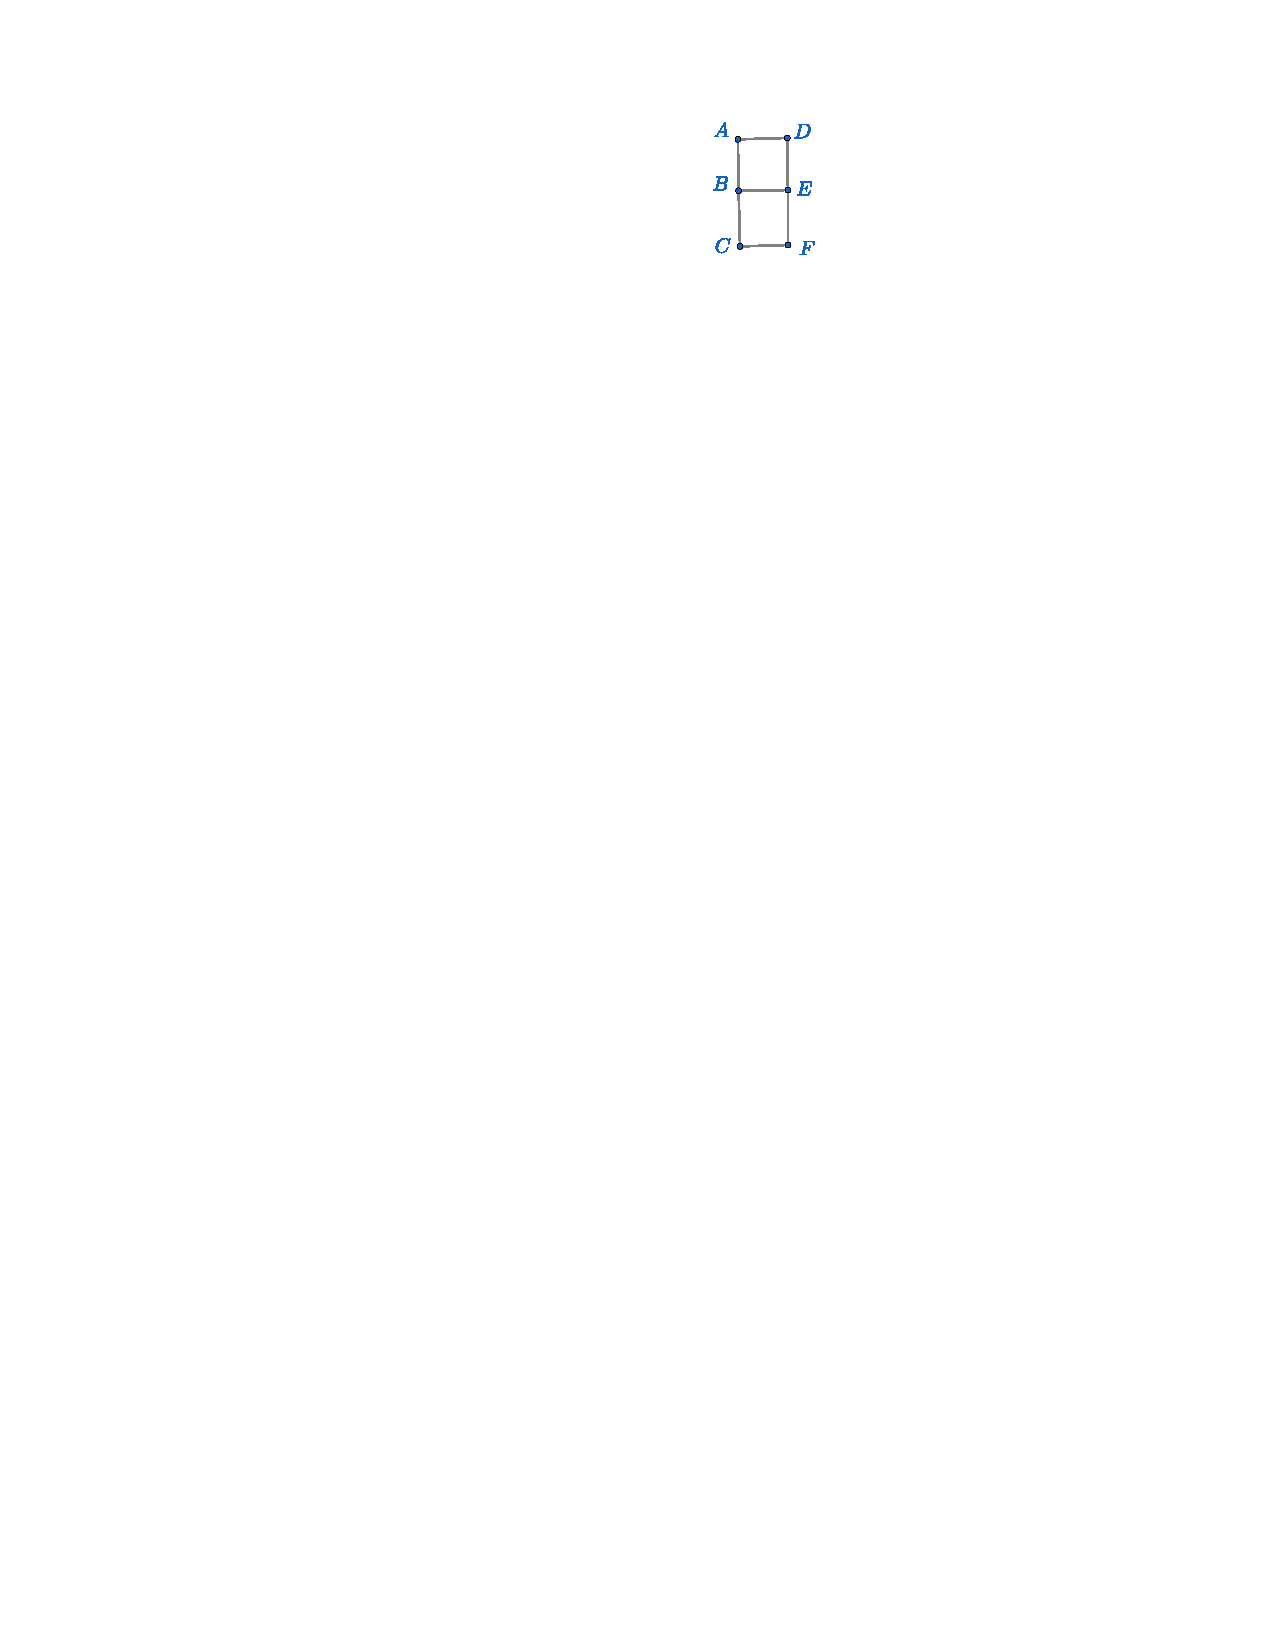
\includegraphics[width=\textwidth]{pics/sparse_relaxation/a_MD.pdf}
  \caption*{(a)}
 \end{minipage}
 \hspace{0.08\textwidth}
 \begin{minipage}[t]{0.15\textwidth}
  \centering
  
\includegraphics[width=\textwidth]{pics/sparse_relaxation/b_MD.pdf}
  \caption*{(b)}
 \end{minipage}
 \hspace{0.08\textwidth}
 \begin{minipage}[t]{0.15\textwidth}
  \centering
  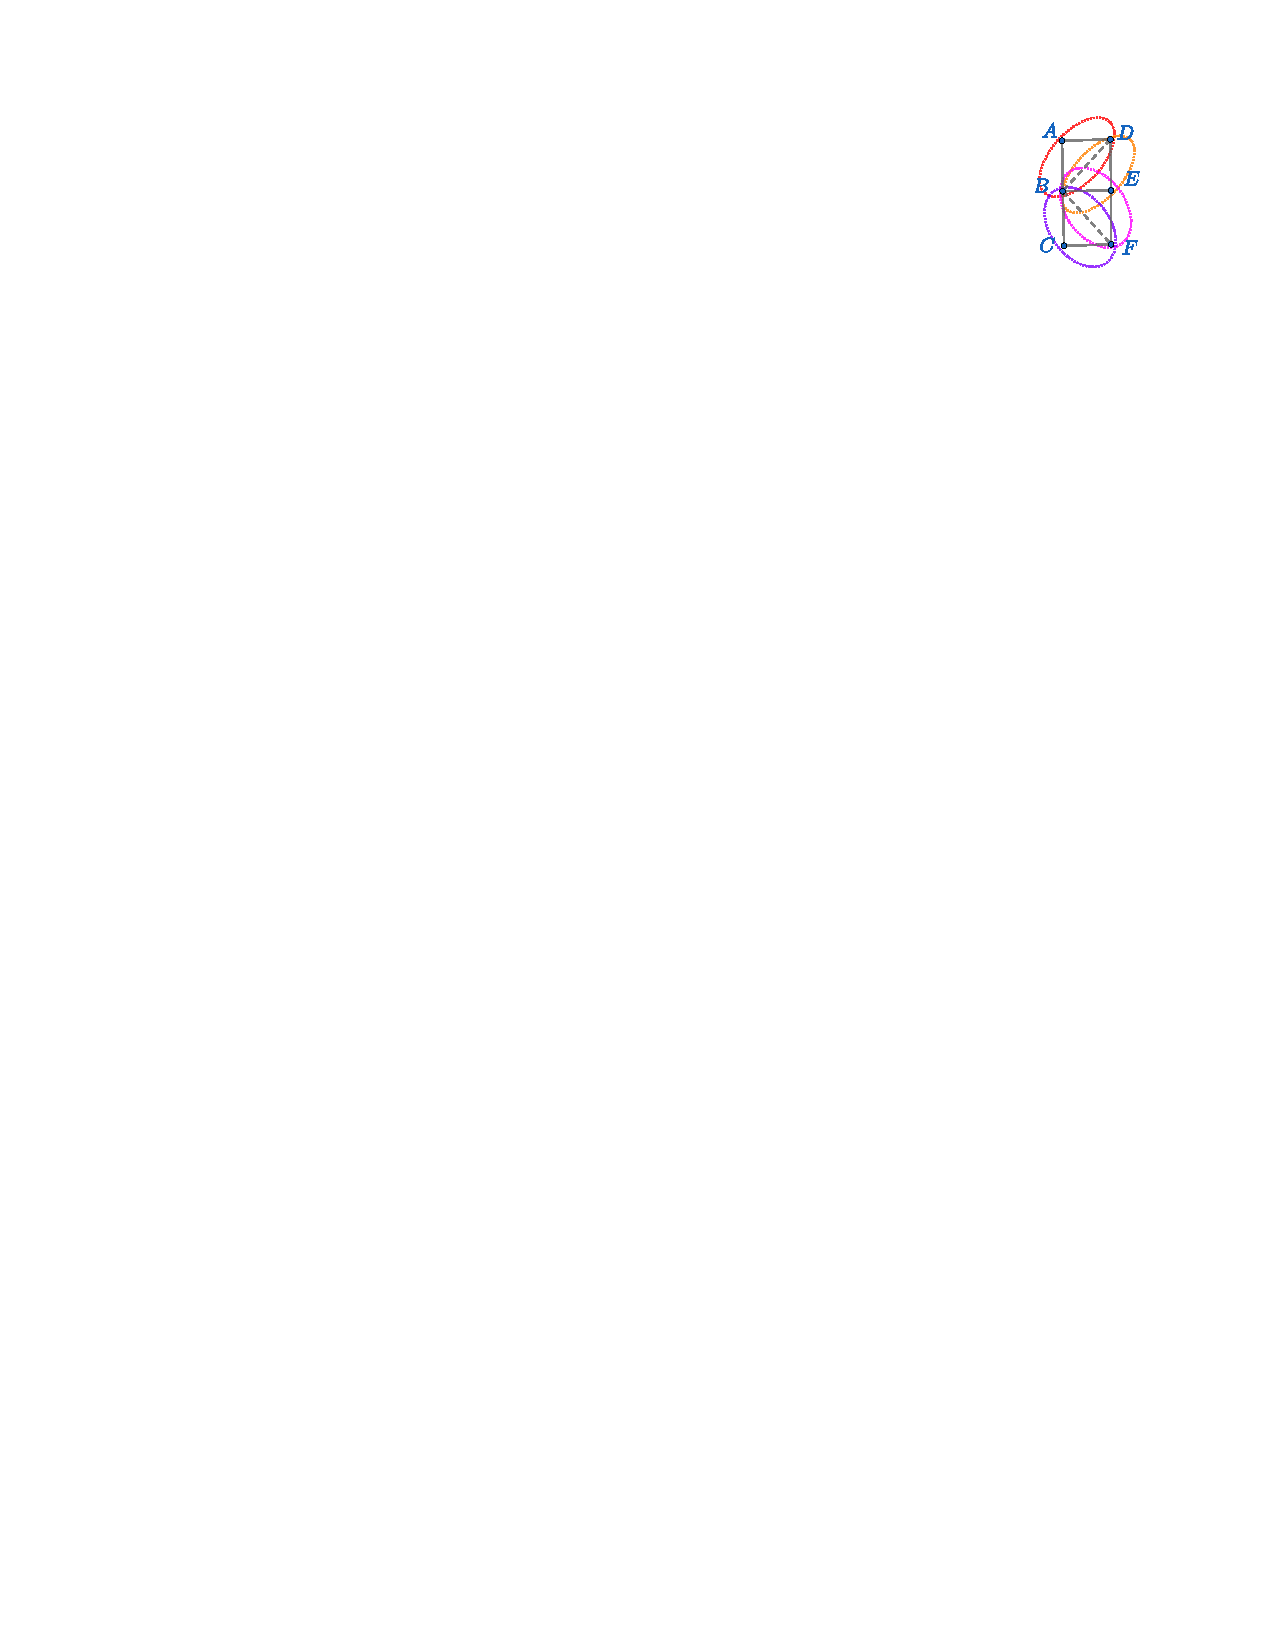
\includegraphics[width=\textwidth]{pics/sparse_relaxation/c_MD.pdf}
  \caption*{(c)}
 \end{minipage}
 \caption{An example of a chordal extension and its maximal cliques. (a) non-chordal. 
 (b) MD chordal extension. (c) maximal cliques. Adapted
 from \cite{Kang_2025Global}.}
 \label{fig:chordal_extension_cliques}
\end{figure}

\paragraph{Chain-like sparsity of trajectory optimization}
For the motion planning formulation of Section 
\ref{sec:discrete_motion_planning_of_rigid_body_systems}, the vectorized 
decision variables can be ordered as
\begin{equation}
    \bm{z}=
    \begin{bmatrix}
    \bm{Y}_0&
    \bm{U}_1&
    \bm{\lambda}_1&
    \bm{Y}_1&
    \cdots&
    \bm{U}_N&
    \bm{\lambda}_N&
    \bm{Y}_N
    \end{bmatrix}^{\top}.
 \label{eq:trajectory_decision_vector}
\end{equation}
\cite{Kang_2026Fast} defines the index set \(\mathcal I_k\), which 
selects the scalar variables of the \(k\)-th
trajectory clique,
\begin{equation}
 \bm{z}(\mathcal I_k)=
 \begin{bmatrix}
 \bm{Y}_{k-1}&\bm{U}_k&\bm{\lambda}_k&\bm{Y}_k
 \end{bmatrix}^{\top},
 \qquad k=1,\ldots,N.
 \label{eq:trajectory_clique}
\end{equation}
For multibody rigid-body systems, each link constraint 
and stage cost for transition \(k\) is contained inside \(\mathcal I_k\).
Additionally, the temporal cliques satisfy
\begin{equation}
 \bigcup_{k=1}^{N} \mathcal I_k=\{1,\ldots,n_z\},
 \qquad
 \left(\bigcup_{i=1}^{k-1}\mathcal I_i\right)\cap \mathcal I_k
 =\mathcal I_{k-1}\cap \mathcal I_k,
 \quad k=2,\ldots,N.
 \label{eq:chain_sparsity_condition}
\end{equation}
Their adjacent overlap contains the shared boundary state \(\bm{Y}_{k-1}\). Therefore,
the property \eqref{eq:chain_sparsity_condition} results from the Markov structure 
of the discretized dynamics
\cite{Sangli2025}.

Figure~\ref{fig:temporal_clique_sparsity} illustrates the chain-like sparsity
pattern for the clique \eqref{eq:trajectory_clique} and the
resulting multi-block SDP, forming a chain-like graph. Thereby,
\(\psi(\bm{Y}_{k-1},\bm{U}_k,\bm{\lambda}_k)\) denotes the stage cost,
\(\mathcal{D}(\bm{Y}_k,\bm{Y}_{k-1},\bm{U}_k,\bm{\lambda}_k)=0\) the polynomial
equality constraints, and \(H(\bm{Y}_k,\bm{U}_k,\bm{\lambda}_k)\geq0\) the polynomial inequality constraints.

\begin{figure}[!ht]
 \centering
 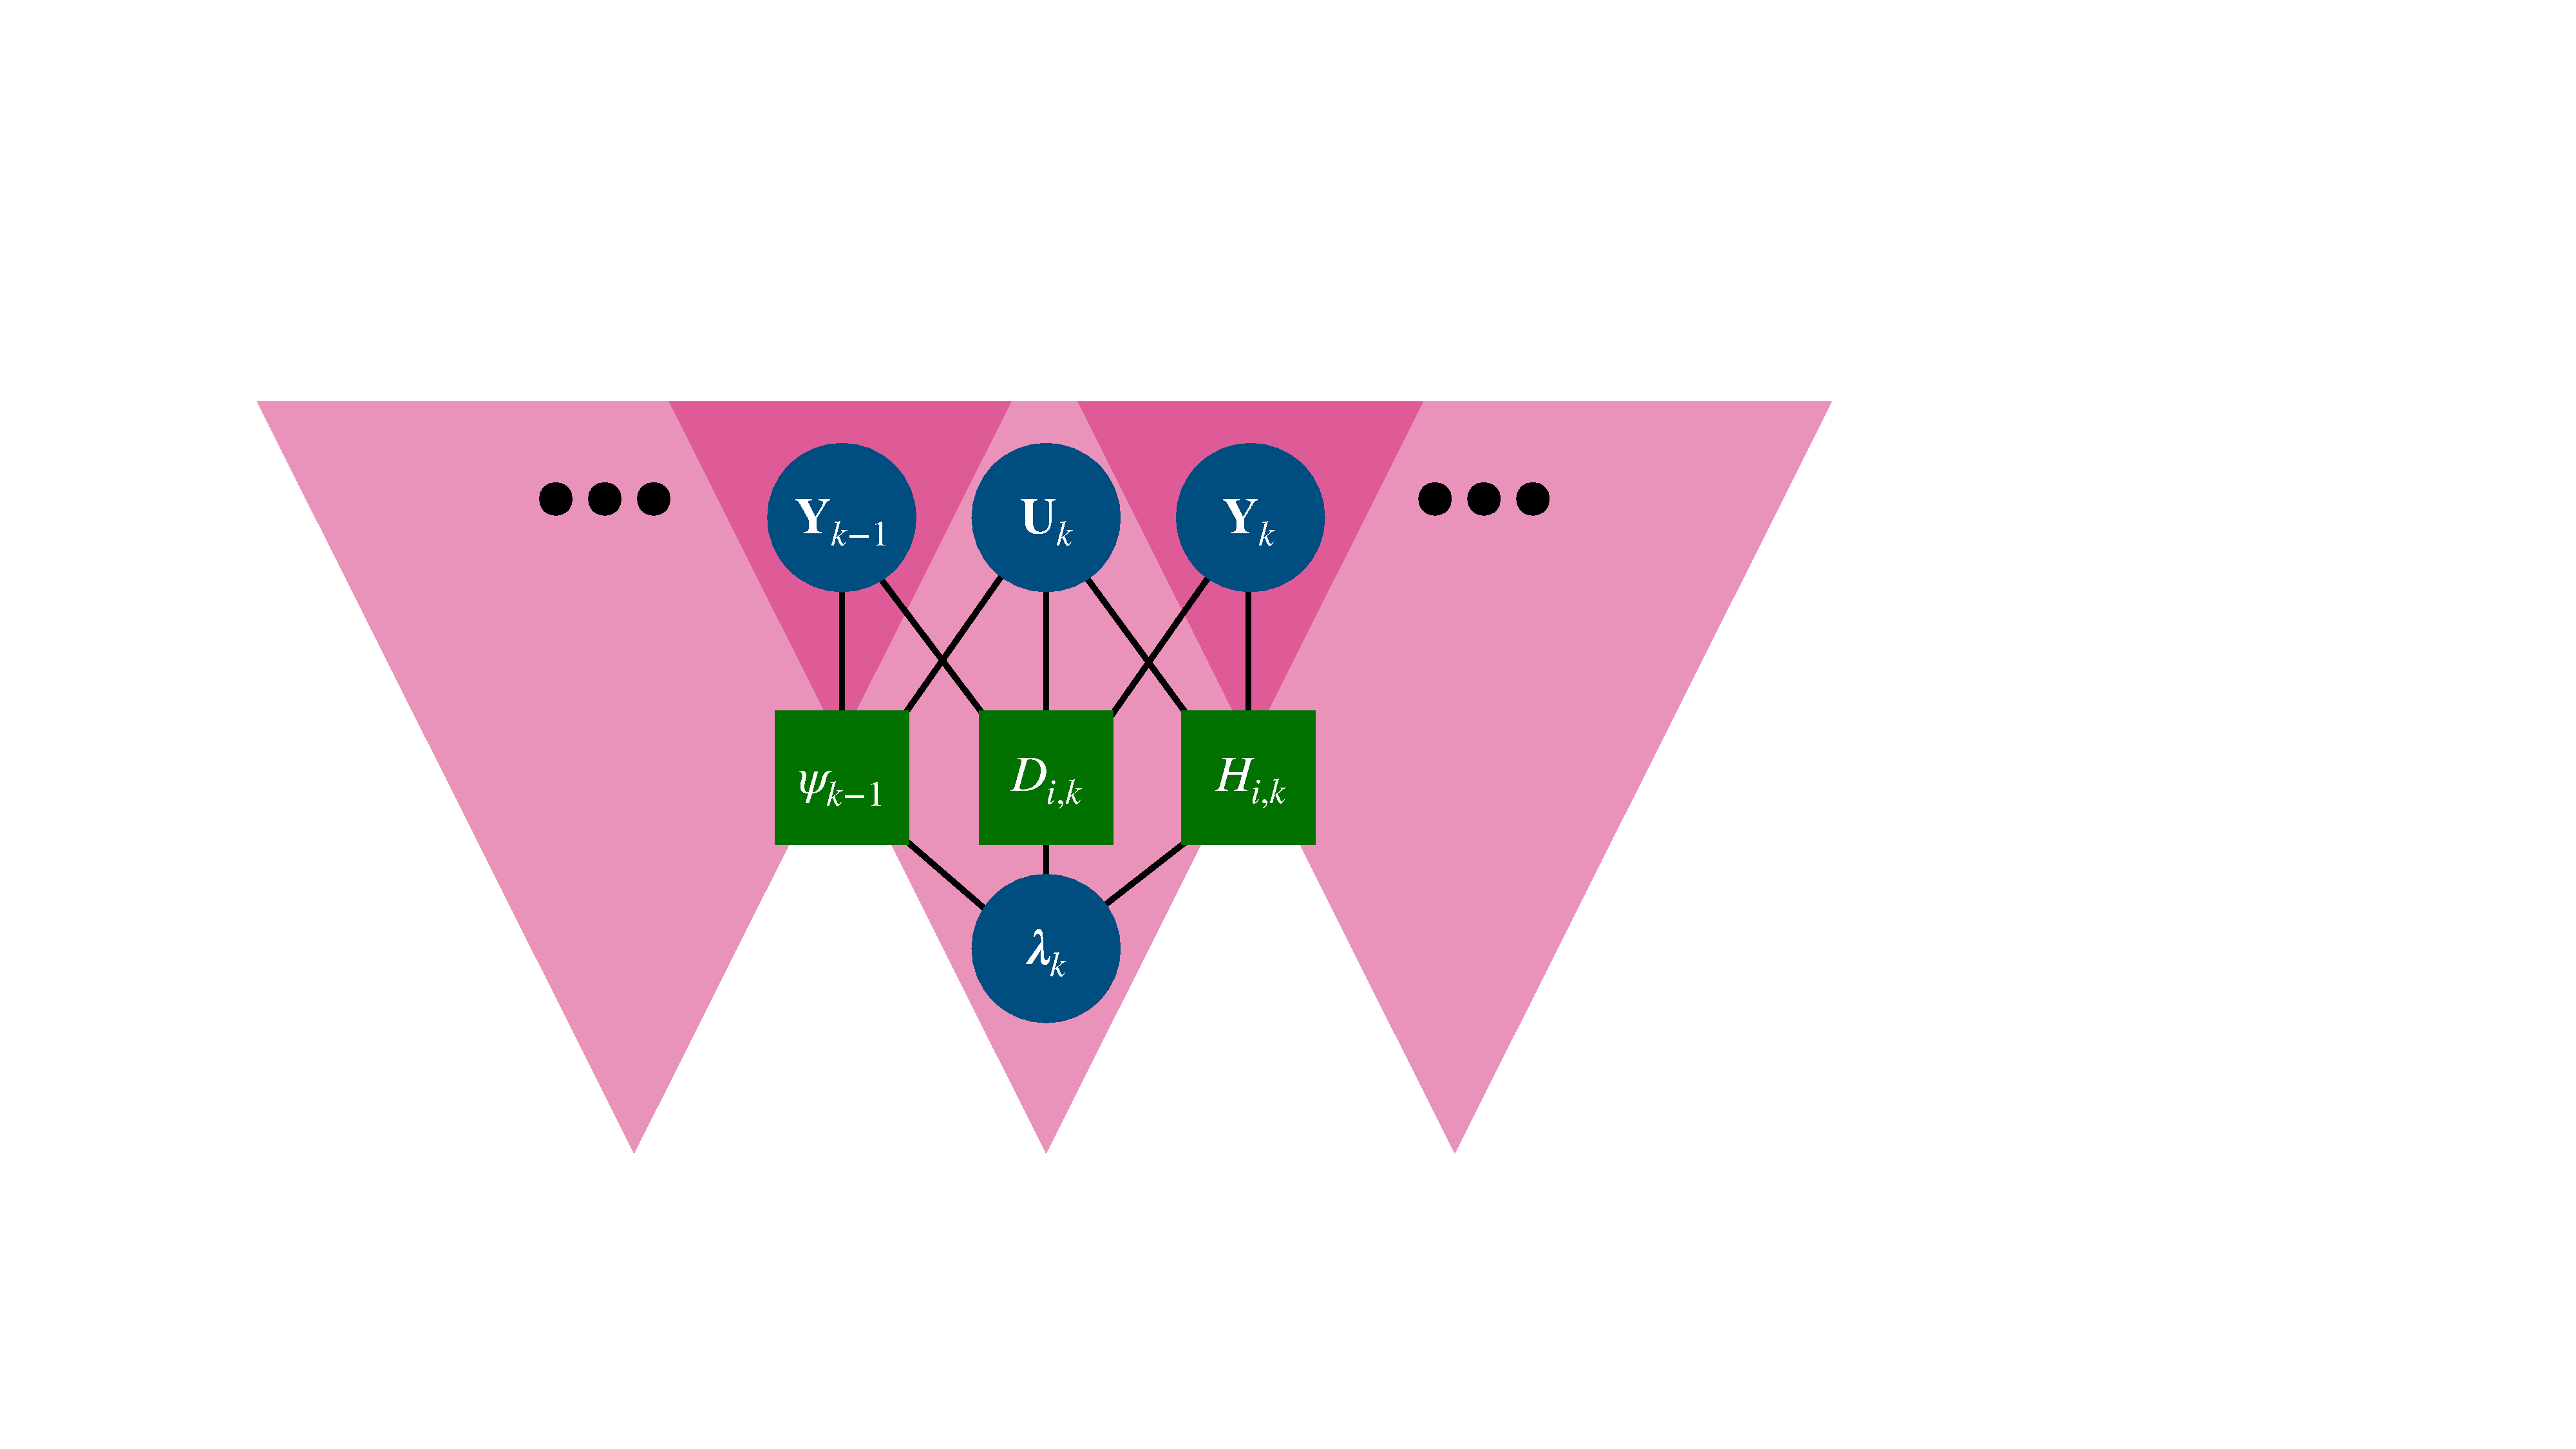
\includegraphics[width=0.6\textwidth]
 {./pics/sparse_relaxation/I_k.pdf}
 \caption{Illustration of a chain-like sparsity pattern.
 Adapted from \cite{Kang_2026Fast}.}
 \label{fig:temporal_clique_sparsity}
\end{figure}

\paragraph{Multibody rigid-body-specific sparsity}
Many robotic systems have local dependencies. 
\cite{Kang_2025Global} gives the example of a 
one-dimensional two-link chain in discrete time 
with the three states $x_{1,k}, x_{2,k}, x_{3,k}$ and the corresponding
control inputs $u_{1,k},u_{2,k},u_{3,k}$,
\begin{align}
&x_{1,k+1} = x_{1,k}+u_{1,k},\\
&x_{2,k+1} = x_{2,k}+u_{2,k},\\
&x_{3,k+1} = x_{3,k}+u_{3,k},\\
&(x_{1,k}-x_{2,k})^2 = r^2, \\
&(x_{2,k}-x_{3,k})^2 = r^2.
\end{align}
Using the chain-like sparsity condition
\eqref{eq:chain_sparsity_condition} therefore gives the nine-variable clique vector
\begin{equation}
\bm{z}(\mathcal I_k^{\mathrm{full}})
=
\begin{bmatrix}
x_{1,k}&x_{2,k}&x_{3,k}&x_{1,k+1}&x_{2,k+1}&x_{3,k+1}&u_{1,k}&u_{2,k}&u_{3,k}
\end{bmatrix}^{\top}.
\end{equation}
\cite{Kang_2025Global} elaborates that each input affects only its corresponding 
state and the geometric constraints couple only neighboring states.
Therefore, this clique vector can be decomposed further into
\begin{align}
\bm{z}(\mathcal I_{\mathrm{dyn},i,k})
&=\begin{bmatrix}x_{i,k}&x_{i,k+1}&u_{i,k}\end{bmatrix}^{\top},
&&i=1,2,3,\\
\bm{z}(\mathcal I_{\mathrm{geom},i,m})
&=\begin{bmatrix}x_{i,m}&x_{i+1,m}\end{bmatrix}^{\top},
&&i=1,2,\quad m\in\{k,k+1\}.
\end{align}
In consequence, the original clique of size nine is replaced by three 
cliques of size three and four cliques of size two.

\paragraph{Sparse Moment--SOS relaxation}
After defining the \(N_{\mathrm{cl}}\) variable cliques
\(\mathcal I_1,\ldots,\mathcal I_{N_{\mathrm{cl}}}\),
\(p(\bm{z})=\sum_{i=1}^{N_{\mathrm{cl}}}p_i(\bm{z}(\mathcal I_i))\) and every
constraint polynomial is assigned to a clique containing all of its variables,
the $\kappa$-order moment relaxation problem \eqref{eq:moment_relaxation_comparison}
can be solved. For the sparse Moment-SOS relaxation, the moment and
localizing conditions are imposed separately on the local monomial bases \cite{Kang_2025Global}.
Consequently, instead of one matrix of dimension
\(\binom{n_z+\kappa}{\kappa}\), the sparse relaxation contains blocks of
dimension \(\binom{|\mathcal I_i|+\kappa}{\kappa}\). Using the chain-like cliques
\eqref{eq:trajectory_clique}, its size remains independent of \(N\) if the
per-stage model size is fixed. Only the number of blocks grows linearly with
\(N\) \cite{Kang_2026Fast}.

Figure~\ref{fig:dense_sparse_moment_comparison} illustrates an example from
\cite{Kang_2025Global}: a reduction for
a POP with two variables \(\bm{x}=(x_1,x_2)\) and relaxation order
\(\kappa=2\). The dense moment matrix has dimension
\(\binom{2+2}{2}=6\). If the variables are separated into the cliques
\(\{x_1\}\) and \(\{x_2\}\), the sparse relaxation instead contains two moment
matrices of dimension \(\binom{1+2}{2}=3\). Consequently, one \(6\times6\)
positive-semidefinite constraint is replaced by two \(3\times3\)
positive-semidefinite constraints \cite{Kang_2025Global}.

\begin{figure}[!ht]
 \centering
 \begin{minipage}[t]{0.44\textwidth}
  \centering
  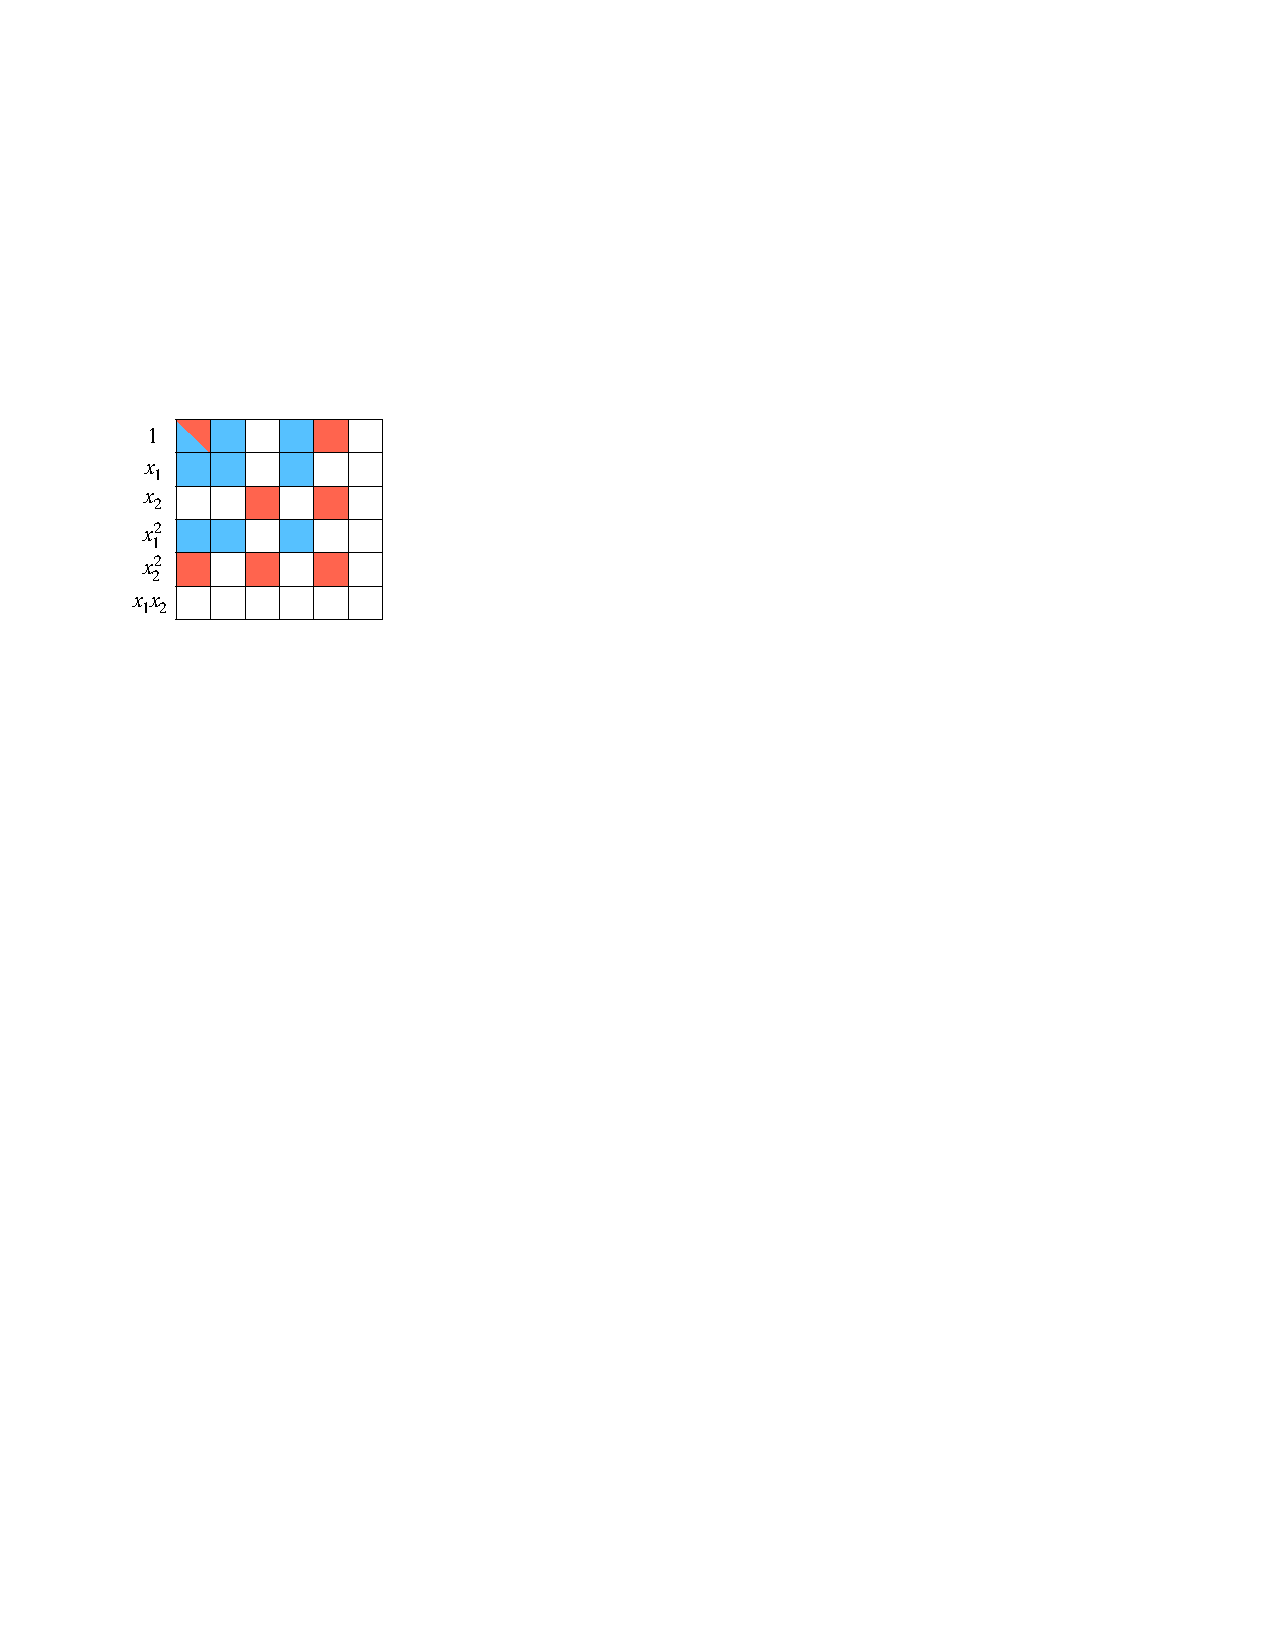
\includegraphics[width=\textwidth]{pics/sparse_relaxation/dense_moment_relaxation.pdf}
  \caption*{(a) Dense Moment Relaxation}
 \end{minipage}
 \begin{minipage}[t]{0.25\textwidth}
  \centering
  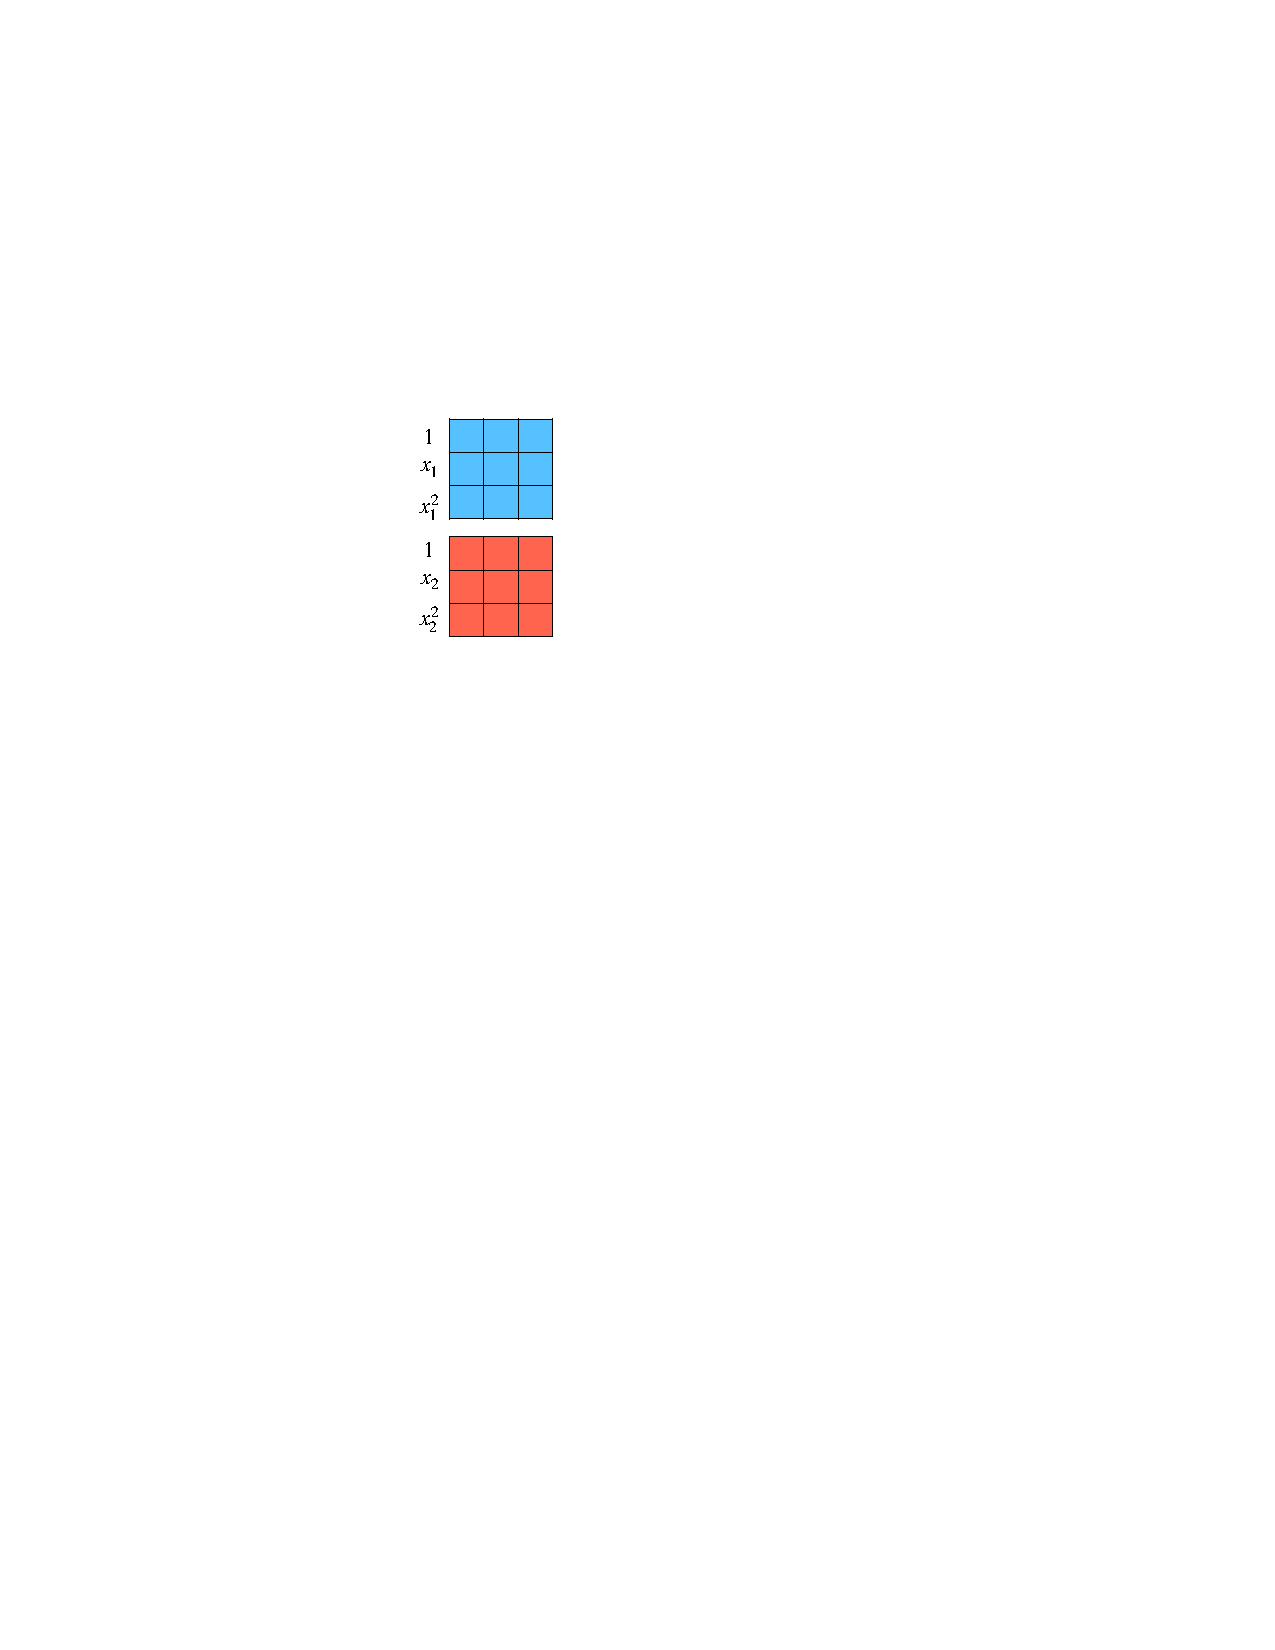
\includegraphics[width=\textwidth]{pics/sparse_relaxation/sparse_moment_relaxation.pdf}
  \caption*{(b) Sparse Moment Relaxation}
 \end{minipage}
 \caption{Comparison of dense and sparse moment matrices for a two-variable POP
 at relaxation order \(\kappa=2\). Reproduced from
 \cite{Kang_2025Global}.}
 \label{fig:dense_sparse_moment_comparison}
\end{figure}

At a fixed order $\kappa$, the sparse lower-bound may
be further away from the optimal solution $p^*$ than the dense bound. 
Still, if all optimal clique moment matrices have rank one, a globally optimal 
trajectory $\bm{z}^*$ can be extracted. However, rank one of only the first
clique does not certify the complete horizon. Following \cite{Sangli2025}, proximity to rank one is
evaluated by
\begin{equation}
 \delta_k:=\frac{\nu_{2,k}}{\nu_{1,k}},
 \qquad
 \delta_{\max}:=\max_{k=1,\ldots,N_{\mathrm{cl}}}\delta_k.
 \label{eq:numerical_rank_metric}
\end{equation}
Here, 
\(\nu_{1,k}\geq\nu_{2,k}\geq\cdots\geq0\) are the eigenvalues of
\(\bm{M}_{\kappa,k}\). \(\delta_{\max}\) close to zero indicates an approximately rank-one solution.
 Nevertheless, it remains a numerical tightness diagnostic and is not an exact certificate.

\paragraph{Sparse Polynomial Optimization Toolbox (SPOT)}
The sparse Moment--SOS relaxations in this thesis are constructed 
using the Sparse Polynomial Optimization Toolbox (SPOT) developed by 
\cite{Kang_2025Global}. Given a POP, SPOT automatically constructs its 
correlative sparsity graph, applies a chordal extension, identifies 
the maximal variable cliques, groups the polynomial constraints, and 
generates the corresponding sparse moment or SOS relaxation. For both 
CS and TS, SPOT provides maximal (MAX), minimum-degree (MD), and minimum-fill 
(MF) chordal-extension options, as well as user-defined (SELF) cliques. TS further 
decomposes the monomial bases within the variable cliques, but is not considered 
in this thesis, because of limited computational capabilities. 
In this thesis, the controlled 3D-pendulum of Section \ref{sec:discrete_3D_pendulum} uses automatic CS with the MD 
extension, whereas the Acrobot of Section \ref{subsection:discrete_Acrobot} uses problem-specific SELF cliques. 
Their exact clique constructions and relaxation orders are specified 
in the following sections.

\newpage

\section{Discrete Motion Planning for the 3D-Pendulum}
\label{sec:discrete_motion_planning_3d_pendulum}

In order to optimize the trajectory of the 3D pendulum, the discrete motion planning 
problem \eqref{eq:general_motion_optimization} has to be formulated as a 
polynomial optimization problem (POP), using the derived discrete Lie group dynamics of the
3D pendulum in Section~\ref{sec:discrete_3D_pendulum}. The optimization variables are the entries of
\(\bm{R}_0,\ldots,\bm{R}_N\), \(\bm{F}_0,\ldots,\bm{F}_{N-1}\), and the control parameters
\(\bm{u}_{p,1},\ldots,\bm{u}_{p,N-1}\), given \cite{Lee2008} definition of the control moment
\begin{equation}
    \bm{u}_k=\bm{R}_k^{\top}\bm{e}_3\times \bm{u}_{p,k}.
\end{equation}
For improved numerical conditioning, the variables have to be scaled to the range \([-1,1]\). 
Therefore, the control input is scaled by the scalar control limit as

\begin{equation}
    \bm{u}_{p,k}
    =u_{\max}\bar{\bm{u}}_{p,k},
    \qquad
    u_{\max}>0,
    \label{eq:u_scaling_3d_pendulum}
\end{equation}
so that the normalized Euclidean control bound becomes
\begin{align}\label{eq:u_bound_3d_pendulum}
    1-\bar{\bm{u}}_{p,k}^{\top}\bar{\bm{u}}_{p,k}\geq0.
\end{align}
In contrast, the entries of \(\bm{R}_k\) and \(\bm{F}_k\) are already bounded by the Lie-group constraints 
\eqref{eq:so3_polynomial_constraints}.

\cite{Kang_2026Fast} defines the cost function as a weighted sum of the terminal and stage costs 
\begin{equation}
    \begin{aligned}
    J_{\mathrm{LQR}}
    &=
    P_f
    \left(\bm{x}_N-\bm{x}_f\right)^\top
    \bm{Q}_x
    \left(\bm{x}_N-\bm{x}_f\right)
    \\
    &\quad+
    \sum_{k=0}^{N-1}
    \left\{
    \left(\bm{x}_k-\bm{x}_f\right)^\top
    \bm{Q}_x
    \left(\bm{x}_k-\bm{x}_f\right)
    +
    \bm{u}_k^\top \bm{Q}_u \bm{u}_k
    \right\},
    \end{aligned}
    \label{eq:lqr_style_loss}
\end{equation}
where $\bm{Q}_x$ and $\bm{Q}_u$ are the identity matrices after rescaling of the variables. 
In addition to \eqref{eq:lqr_style_loss}, this thesis uses individual weights $w_R$, $w_F$ for
the terminal costs and $\alpha_R$, $\alpha_F$, $w_u$ for
the stage costs.  

In the next step, the constraints given by \eqref{eq:general_motion_optimization} have to be 
identified for the 3D-pendulum. The equality constraints $\mathcal{D}$ are given by the discrete 
forced dynamics \eqref{eq:forced_3D_pendulum_EL_dynamics} and the 
kinematics update \eqref{eq:forced_3D_pendulum_EL_kinematics}. Moreover, the
Lie-group constraints $\mathcal{Y}$ defined in Section~\ref{sec:discrete_motion_planning_of_rigid_body_systems}
by \eqref{eq:so3_polynomial_constraints} have to be included for $\bm{R}_k$ and $\bm{F}_k$.
Finally, by using the inequality relation $\mathcal{H}$ given in \cite{GallierQuaintance2020LinearAlgebra}, 
\begin{align}
    \operatorname{tr}(\bm{F}_k)=1+2\cos(\Delta\theta_k)
\end{align}
the relative rotation during one step $\bm{F}_k$ is bounded by the angle $0 \leq \Delta\theta_{\max} \leq \pi$, and
the control input by \eqref{eq:u_bound_3d_pendulum}. In summary, the full controlled 
3D-pendulum POP is defined as
\begingroup
\footnotesize
\begin{subequations}
\label{eq:controlled_3d_pendulum_pop}
\begin{align}
p_{\mathrm{P}}^{\star}
=
\min_{\substack{
\{\bm{R}_k\}_{k=0}^{N},\,\{\bm{F}_k\}_{k=0}^{N-1}\\[-0.2em]
\{\bar{\bm{u}}_{p,k}\}_{k=1}^{N-1}}}
\quad
&w_R\left\|\bm{R}_N-\bm{R}_N^{\mathrm{des}}\right\|_F^2
+w_F\left\|\bm{F}_{N-1}-\bm{F}^{\mathrm{des}}\right\|_F^2
\notag\\[-0.9em]
&+\alpha_R \sum_{k=0}^{N-1}
\left\|\bm{R}_k-\bm{R}_N^{\mathrm{des}}\right\|_F^2
+\alpha_F \sum_{k=0}^{N-2}
\left\|\bm{F}_k-\bm{F}^{\mathrm{des}}\right\|_F^2
\notag\\[0.4em]
&+\frac{1}{w_u} \sum_{k=1}^{N-1}\left\|\bar{\bm{u}}_{p,k}\right\|_2^2
\label{eq:controlled_3d_pendulum_pop_objective}
\\[0.2em]
\hspace{-0.9em}\text{s.t.}\quad
&\hspace{-0.9em}\begin{aligned}
\frac{1}{h}\left(
\bm{F}_{k+1}\bm{J}_d-\bm{J}_d\bm{F}_{k+1}^{\top}-\bm{J}_d\bm{F}_k+\bm{F}_k^{\top}\bm{J}_d
\right)
&=h\left(\bm{\tau}_{g,k+1}+\bm{u}_{k+1}\right)^{\wedge}
\end{aligned},
\label{eq:controlled_3d_pendulum_pop_dynamics}
\\[0.8em]
&\hspace{-0.9em}\begin{aligned}
\bm{R}_{k+1}&=\bm{R}_k\bm{F}_k
\end{aligned},
\label{eq:controlled_3d_pendulum_pop_kinematics}
\\[0.8em]
&\hspace{-0.9em}\begin{aligned}
&\|\bm{r}_{1,k}\|_2^2-1=\|\bm{r}_{2,k}\|_2^2-1=\|\bm{r}_{3,k}\|_2^2-1=0,\\[-0.2em]
&\bm{r}_{1,k}^{\top}\bm{r}_{2,k}=\bm{r}_{2,k}^{\top}\bm{r}_{3,k}
=\bm{r}_{1,k}^{\top}\bm{r}_{3,k}=0,\\[-0.2em]
&\bm{r}_{1,k}\!\times \bm{r}_{2,k}-\bm{r}_{3,k}
=\bm{r}_{2,k}\!\times \bm{r}_{3,k}-\bm{r}_{1,k}
=\bm{r}_{3,k}\!\times \bm{r}_{1,k}-\bm{r}_{2,k}=\bm{0}_{3\times1},
\end{aligned}
\label{eq:controlled_3d_pendulum_pop_so3_R}
\\[0.8em]
&\hspace{-0.9em}\begin{aligned}
&\|\bm{f}_{1,k}\|_2^2-1=\|\bm{f}_{2,k}\|_2^2-1=\|\bm{f}_{3,k}\|_2^2-1=0,\\[-0.2em]
&\bm{f}_{1,k}^{\top}\bm{f}_{2,k}=\bm{f}_{2,k}^{\top}\bm{f}_{3,k}
=\bm{f}_{1,k}^{\top}\bm{f}_{3,k}=0,\\[-0.2em]
&\bm{f}_{1,k}\!\times \bm{f}_{2,k}-\bm{f}_{3,k}
=\bm{f}_{2,k}\!\times \bm{f}_{3,k}-\bm{f}_{1,k}
=\bm{f}_{3,k}\!\times \bm{f}_{1,k}-\bm{f}_{2,k}=\bm{0}_{3\times1},
\end{aligned}
\label{eq:controlled_3d_pendulum_pop_so3_F}
\\[0.8em]
&\hspace{-0.9em}\begin{aligned}
\frac{\operatorname{tr}(\bm{F}_k)-1}{2}
&\geq \cos(\Delta\theta_{\max})
\end{aligned},
\label{eq:controlled_3d_pendulum_pop_step_bound}
\\[0.8em]
&\hspace{-0.9em}\begin{aligned}
1-\bar{\bm{u}}_{p,k}^{\top}\bar{\bm{u}}_{p,k}&\geq0
\end{aligned},
\label{eq:controlled_3d_pendulum_pop_control_bound}
\\[0.8em]
&\hspace{-0.9em}\begin{aligned}
\bm{R}_0&=\bm{R}^{\mathrm{init}},
\qquad \bm{F}_0=\bm{F}^{\mathrm{init}}
\end{aligned}.
\label{eq:controlled_3d_pendulum_pop_initial}
\end{align}
\end{subequations}
\endgroup
with the initial conditions \(\bm{R}^{\mathrm{init}}\) and \(\bm{F}^{\mathrm{init}}\).
Here, \eqref{eq:controlled_3d_pendulum_pop_dynamics} holds for
\(k=0,\ldots,N-2\), \eqref{eq:controlled_3d_pendulum_pop_kinematics}
and \eqref{eq:controlled_3d_pendulum_pop_step_bound} hold for
\(k=0,\ldots,N-1\), \eqref{eq:controlled_3d_pendulum_pop_so3_R}
holds for \(k=0,\ldots,N\), \eqref{eq:controlled_3d_pendulum_pop_so3_F}
holds for \(k=0,\ldots,N-1\), and
\eqref{eq:controlled_3d_pendulum_pop_control_bound} holds for
\(k=1,\ldots,N-1\).
Moreover, \(h\) is the time step, \(\bm{J}_d\) is the nonstandard inertia matrix \eqref{eq:non-standard_inertia},
and $\bm{\tau}_{g,k}$ denotes the gravity moment in the body-fixed frame \eqref{eq:3d_pendulum_gravity_moment}.
The definition of \(\bm{r}_{i,k}\) and \(\bm{f}_{i,k}\) is given in \eqref{eq:so3_polynomial_constraints}.
Finally, \eqref{eq:controlled_3d_pendulum_pop} gives the full POP of the 3d-pendulum with 
polynomials until degree 2.

In order to construct the sparse moment relaxation, the chain-like sparsity 
structure of the 3D-pendulum POP has to be identified. The local decision vector
associated with the pendulum clique index set \(\mathcal I_k^{\mathrm{P}}\) is ordered as
\begin{align}\label{eq:3d_pendulum_sparse_clique}
    \bm{z}_{\mathrm{P}}(\mathcal I_k^{\mathrm{P}})
    =
    [\bm{R}_{k+1} \quad \bm{F}_{k+1} \quad \bm{R}_{k} \quad \bm{F}_{k} \quad \bar{\bm{u}}_{p,k+1} ]^{\top},
    \qquad k=0,\ldots,N-2,
\end{align}
which is consistent with the chain-like sparsity condition \eqref{eq:chain_sparsity_condition}.
Thereby, the dynamics and kinematics only couple neighboring time steps. 
Therefore, the clique vector \(\bm{z}_{\mathrm{P}}(\mathcal I_k^{\mathrm{P}})\)
contains \(n_{\mathrm{cl}}=39\) scalar variables.
\cite{Sangli2025} identifies for a clique size of \(n_{\mathrm{cl}}\), the order-\(\kappa\) moment matrix
dimension as
\begin{equation}
s(n_{\mathrm{cl}},\kappa)
=\binom{n_{\mathrm{cl}}+\kappa}{\kappa}.
\label{eq:moment_size}
\end{equation}
Consequently, at $\kappa=2$, a 39-variable interior clique
\(\bm{z}_{\mathrm{P}}(\mathcal I_k^{\mathrm{P}})\) yields $s(39,2)=820$.
The corresponding moment matrix therefore has size $820\times820$. In
contrast, the full decision vector contains
\[
 n_{z,\mathrm{P}}=9(N+1)+9N+3(N-1)=21N+6
\]
variables. A dense second-order relaxation would consequently require a moment
matrix of size
\[
s(n_{z,\mathrm{P}},2)=\binom{21N+8}{2}.
\]
For the implemented horizon $N=20$, this corresponds to a
$91\,378\times91\,378$ moment matrix, which is computationally not feasible. 
Nevertheless, the spare relaxation \eqref{eq:3d_pendulum_sparse_clique} 
consists of bigger miment matrices, compared to the moment matrices constructed using 
MD, which will be used for the Evaluation.
In the following Section \ref{sec:3d_pendulum_optimization_results},
SPOT is used to construct the second-order sparse moment relaxation from the 3D-pendulum's POP 
\eqref{eq:controlled_3d_pendulum_pop} \cite{Kang_2025Global}. The resulting SDP is solved with the interior-point solver
MOSEK \cite{MOSEK}. The scalar equations used in the implementation are listed in
Appendix~\ref{app:controlled_3d_pendulum_scalar_pop}. Finally, the implementation is documented 
in the GitHub repository \cite{Elshani2026CTO_GitHub}.

\section{Discrete Motion Planning for an Acrobot}
\label{sec:discrete_motion_planning_acrobot}

The following section applies the discrete motion planning formulation of
Section \ref{sec:discrete_motion_planning_of_rigid_body_systems} 
to the controlled Acrobot derived in Section \ref{subsection:discrete_Acrobot}. 
First, the trajectory optimization problem is solved in Section 
\ref{sec:trajectory_optimization_via_sdp_relaxation} 
using a sparse semidefinite relaxation. Subsequently, the same relaxation is 
embedded into a model predictive control framework to obtain a 
closed-loop controller in Section \ref{sec:acrobot_trajectory_optimization_SDP_MPC}.

\subsection{Trajectory Optimization via SDP Relaxation}
\label{sec:trajectory_optimization_via_sdp_relaxation}
To optimize the Acrobot trajectory, the discrete motion planning
problem \eqref{eq:general_motion_optimization} has to be formulated as a POP using
the controlled discrete Euler-Lagrange equations of Section \ref{subsection:discrete_Acrobot}. 
For the two links $i=1,2$, the planar rotations are represented around the z-axis by 
\eqref{eq:so2_polynomial_constraints}.
The Acrobot model in maximal coordinates contains additional 
velocity variables $\bm{v}_{i,k}\in\mathbb R^2$, which results in a higher number of optimization variables.
Instead, the maximal coordinate model can be reduced by eliminating the
translational positions and velocities while the constraints still remain
polynomial. Therefore, the 
holonomic constraints \eqref{eq:acrobot_base_constraint} and 
\eqref{eq:acrobot_elbow_constraint} eliminate the center-of-mass
positions exactly according to
\begin{equation}
\bm{x}_{1,k}=\bm{p}_0-\bm{R}_{1,k}\bm{\rho}_{1,0},
\qquad
\bm{x}_{2,k}=\bm{p}_0+\bm{R}_{1,k}(\bm{\rho}_{1,12}-\bm{\rho}_{1,0})
               -\bm{R}_{2,k}\bm{\rho}_{2,12}.
\label{eq:acrobot_eliminated_positions}
\end{equation}
Therefore, the velocity $\bm{v}_{i,k}$ can be approximated from the rotations by  
\begin{subequations}\label{eq:velocity_approximation_rotations}
\begin{align}
    \bm{v}_{1,k}
    &\approx
    \frac{(\bm{R}_{1,k}-\bm{R}_{1,k+1})\bm{\rho}_{1,0}}{h},
    \label{eq:velocity_approximation_link1}\\
    \bm{v}_{2,k}
    &\approx
    \frac{
        (\bm{R}_{1,k+1}-\bm{R}_{1,k})
        (\bm{\rho}_{1,12}-\bm{\rho}_{1,0})
        -(\bm{R}_{2,k+1}-\bm{R}_{2,k})\bm{\rho}_{2,12}
    }{h}.
    \label{eq:velocity_approximation_link2}
\end{align}
\end{subequations}
substituting \eqref{eq:acrobot_eliminated_positions} into \eqref{eq:acrobot_discrete_translational_velocity}.
In addition, the kinematic update \eqref{eq:acrobot_full_del_shifted_kinematics_1}-\eqref{eq:acrobot_full_del_shifted_kinematics_2} can be rewritten as
\begin{equation}
\bm{R}_{i,k-1}=\bm{R}_{i,k}\bm{F}_{i,k-1}^{\top}.
\label{eq:acrobot_kinematic_substitution}
\end{equation}
Consequently, using \eqref{eq:acrobot_full_del_shifted_kinematics_1}-\eqref{eq:acrobot_full_del_shifted_kinematics_2},
\eqref{eq:acrobot_kinematic_substitution} and \eqref{eq:velocity_approximation_rotations},
the translational dynamics 
\eqref{eq:acrobot_full_del_shifted_translation_1}-\eqref{eq:acrobot_full_del_shifted_translation_2} are reduced to a polynomial form 
\begin{subequations}
\begingroup
\setlength{\jot}{0.35em}
\vspace{-0.3cm}
\begin{align}
    \intertext{\textit{Translation:}}
    \vspace{-0.1cm}
    -\bm{M}_1 \bm{R}_{1,k}
    \bm{A}_{1,k}\bm{\rho}_{1,0}
    -h^2g\bm{M}_1\bm{e}_2
    -h^2\left(\bm{\lambda}_{0,k}+\bm{\lambda}_{12,k}\right)
    &=
    \bm{0},
    \label{eq:acrobot_full_del_shifted_translation_1_reduced}
    \\
\hspace{-2em}
    \bm{M}_2\Bigl[
    \bm{R}_{1,k}
    \bm{A}_{1,k}
    \left(\bm{\rho}_{1,12}-\bm{\rho}_{1,0}\right)
    -\bm{R}_{2,k}
    \bm{A}_{2,k}\bm{\rho}_{2,12}
    \Bigr]
    -h^2g\bm{M}_2\bm{e}_2
    +h^2\bm{\lambda}_{12,k}
    &=
    \bm{0},
    \label{eq:acrobot_full_del_shifted_translation_2_reduced}
\end{align}
\endgroup
\end{subequations}
with $\bm{A}_{i,k}=\bm{F}_{i,k}-2\bm{I}_2+\bm{F}_{i,k-1}^{\top}$.
Therefore, the reduced translational dynamics only depend on the relative rotations
$\bm{F}_{i,k}$ and $\bm{F}_{i,k-1}$, and the attitude $\bm{R}_{i,k}$.
The physical properties of the reduced model are validated and compared to the full model in the 
Appendix \ref{appendix:experimental_details}.

Similar to the 3D pendulum in Section \ref{sec:discrete_motion_planning_3d_pendulum}, 
for numerical conditioning, the control and constraint multipliers are scaled
to the interval $[-1,1]$ componentwise,
\begin{equation}
u_k^{\mathrm{phys}}=u_{\max}\bar u_k,
\qquad
\bm{\lambda}_{0,k}=\lambda_{\max}\bar{\bm{\lambda}}_{0,k},
\qquad
\bm{\lambda}_{12,k}=\lambda_{\max}\bar{\bm{\lambda}}_{12,k}.
\label{eq:acrobot_variable_scaling}
\end{equation}
The normalized control and componentwise multiplier bounds are
\begin{equation}
1-\bar u_k^2\geq0,
\qquad
1-\bigl(\bar{\lambda}_{0,k}^{(j)}\bigr)^2\geq0,
\qquad
1-\bigl(\bar{\lambda}_{12,k}^{(j)}\bigr)^2\geq0,
\quad j=1,2.
\label{eq:acrobot_normalized_bounds}
\end{equation}
Moreover, since
$\tfrac12\operatorname{tr}(\bm{F}_{i,k})=a_{i,k}=\cos(\Delta\theta_{i,k})$,
the relative-rotation bound is
\begin{align}\label{eq:acrobot_normalized_f_bound}
a_{i,k}\geq\cos(\Delta\theta_{i,\max}).
\end{align} 
The entries of $\bm{R}_{i,k}$ and
$\bm{F}_{i,k}$ are already bounded by the $SO(2)$ constraints.

The optimization variables are the entries of
$\bm{R}_{i,0},\ldots,\bm{R}_{i,N}$, $\bm{F}_{i,0},\ldots,\bm{F}_{i,N-1}$, and the normalized
variables $\bar{\bm{\lambda}}_{0,k},\bar{\bm{\lambda}}_{12,k}\in\mathbb R^2$ and
$\bar u_k\in\mathbb R$, $k=1,\ldots,N-1$.
Therefore, the reduced full-horizon decision vector contains $n_{z,\mathrm{A}}^{reduced}=13N-1$
scalar variables, compared to the original $n_{z,\mathrm{A}}^{full}=17N+3$ variables of the full model using position variables $\bm{x_{i,k}}$.


Similar to the 3D-pendulum objective introduced in \eqref{eq:lqr_style_loss}
(see Section \ref{sec:discrete_motion_planning_3d_pendulum}), the Acrobot
objective uses individual terminal weights $w_R,w_F,$ and stage weights 
$\alpha_R,\alpha_F$, and \(w_u\). The multipliers $\bar{\bm{\lambda}}_{0,k}$ and $\bar{\bm{\lambda}}_{12,k}$ 
are not penalized. In the notation of the general problem~\eqref{eq:general_motion_optimization}, 
the equality constraints $\mathcal{D}_i$ consist of the reduced translational 
\eqref{eq:acrobot_full_del_shifted_translation_1_reduced}-\eqref{eq:acrobot_full_del_shifted_translation_2_reduced} 
and rotational dynamics \eqref{eq:forced_acrobot_rotation_link1}-\eqref{eq:forced_acrobot_rotation_link2},
together with the kinematic update 
\eqref{eq:acrobot_full_del_shifted_kinematics_1}-\eqref{eq:acrobot_full_del_shifted_kinematics_2}. 
The SO(2) Lie-group constraints \eqref{eq:so2_polynomial_constraints}
form $\mathcal{Y}_i$, whereas $\mathcal{H}$ contains the increment \eqref{eq:acrobot_normalized_f_bound},
control, and multiplier bounds \eqref{eq:acrobot_normalized_bounds}.
In summary, the
full controlled Acrobot POP is defined as
\begingroup
\footnotesize
\allowdisplaybreaks
\begin{subequations}
\label{eq:controlled_acrobot_pop}
\begin{align}
p_{\mathrm A}^{\star}
=
\min_{\bm{z}_{\mathrm{A}}}
\quad
&w_R\sum_{i=1}^{2}\|\bm{R}_{i,N}-\bm{R}_i^{\mathrm{des}}\|_F^2
+w_F\sum_{i=1}^{2}\|\bm{F}_{i,N-1}-\bm{F}_i^{\mathrm{des}}\|_F^2
\notag\\[-0.1em]
&+\alpha_R\sum_{k=0}^{N-1}\sum_{i=1}^{2}
  \|\bm{R}_{i,k}-\bm{R}_i^{\mathrm{des}}\|_F^2
+\alpha_F\sum_{k=0}^{N-2}\sum_{i=1}^{2}
  \|\bm{F}_{i,k}-\bm{F}_i^{\mathrm{des}}\|_F^2
\notag\\[-0.1em]
&+\frac{1}{w_u}\sum_{k=1}^{N-1}\bar u_k^2
\label{eq:controlled_acrobot_pop_objective}
\\[0.2em]
\hspace{-0.9em}\text{s.t.}\quad
&\hspace{-0.9em}\begin{aligned}
-\bm{M}_1 \bm{R}_{1,k}
\bm{A}_{1,k}\bm{\rho}_{1,0}
-h^2g\bm{M}_1\bm{e}_2
-h^2\left(\bar{\bm{\lambda}}_{0,k}+\bar{\bm{\lambda}}_{12,k}\right)
&=\bm{0}_2
\end{aligned}
\label{eq:controlled_acrobot_pop_translation_1}\\
&\hspace{-0.9em}\begin{aligned}
\bm{M}_2\Bigl[
\bm{R}_{1,k}
\bm{A}_{1,k}
\left(\bm{\rho}_{1,12}-\bm{\rho}_{1,0}\right)
-\bm{R}_{2,k}
\bm{A}_{2,k}\bm{\rho}_{2,12}
\Bigr]
-h^2g\bm{M}_2\bm{e}_2
+h^2\bar{\bm{\lambda}}_{12,k}
&=\bm{0}_2
\end{aligned}
\label{eq:controlled_acrobot_pop_translation_2}\\[0.8em]
&\hspace{-0.9em}\begin{aligned}
&
\hat{\bm{\Pi}}_{1,k}
-\hat{\bm{\Pi}}_{1,k+1}
\\
&\quad
+h
\left[
\left(
\bm{\rho}_{1,0}
\times
\bm{R}_{1,k+1}^{\top}\bar{\bm{\lambda}}_{0,k+1}
\right)
+
\left(
\bm{\rho}_{1,12}
\times
\bm{R}_{1,k+1}^{\top}\bar{\bm{\lambda}}_{12,k+1}
\right)
-u_{\max}\bar u_{k+1}
\right]^{\wedge}
&=\bm{0}
\end{aligned}
\label{eq:controlled_acrobot_pop_rotation_1}
\\
&\hspace{-0.9em}\begin{aligned}
\hat{\bm{\Pi}}_{2,k}
-\hat{\bm{\Pi}}_{2,k+1}
+h
\left[
u_{\max}\bar u_{k+1}
-
\left(
\bm{\rho}_{2,12}
\times
\bm{R}_{2,k+1}^{\top}\bar{\bm{\lambda}}_{12,k+1}
\right)
\right]^{\wedge}
&=\bm{0}
\end{aligned}
\label{eq:controlled_acrobot_pop_rotation_2}\\[0.8em]
&\hspace{-0.9em}\bm{R}_{i,k+1}=\bm{R}_{i,k}\bm{F}_{i,k},
\label{eq:controlled_acrobot_pop_kinematics}\\[0.8em]
&\hspace{-0.9em}c_{i,k}^2+s_{i,k}^2-1=0,
\label{eq:controlled_acrobot_pop_so2_R}\\
&\hspace{-0.9em}a_{i,k}^2+b_{i,k}^2-1=0,
\label{eq:controlled_acrobot_pop_so2_F}\\[0.8em]
&\hspace{-0.9em}a_{i,k}-\cos(\Delta\theta_{i,\max})\geq0,
\label{eq:controlled_acrobot_pop_step_bound}\\
&\hspace{-0.9em}1-\bar u_k^2\geq0,
\label{eq:controlled_acrobot_pop_control_bound}\\
&\hspace{-0.9em}1-\bigl(\bar{\lambda}_{0,k}^{(j)}\bigr)^2\geq0,
\quad
1-\bigl(\bar{\lambda}_{12,k}^{(j)}\bigr)^2\geq0,
\label{eq:controlled_acrobot_pop_multiplier_bound}\\[0.8em]
&\hspace{-0.9em}\begin{gathered}
\bm{F}_{i,0}=\bm{F}_i^{\mathrm{init}},\qquad
\bm{R}_{i,1}=\bm{R}_i^{\mathrm{init}}.
\end{gathered}
\label{eq:controlled_acrobot_pop_initial}
\end{align}
\end{subequations}
\endgroup

\begin{table}[htbp]
\centering
\small
\caption{Index ranges for the constraints in the controlled Acrobot POP.}
\label{tab:controlled_acrobot_pop_indexing}
\begin{tabular}{@{}lll@{}}
\toprule
Constraint & Equation(s) & Indexing \\
\midrule
Translation
& \eqref{eq:controlled_acrobot_pop_translation_1},
  \eqref{eq:controlled_acrobot_pop_translation_2}
& \(k=1,\ldots,N-1\) \\
Rotation
& \eqref{eq:controlled_acrobot_pop_rotation_1},
  \eqref{eq:controlled_acrobot_pop_rotation_2}
& \(k=0,\ldots,N-2\) \\
Kinematics
& \eqref{eq:controlled_acrobot_pop_kinematics}
& \(i=1,2,\; k=0,\ldots,N-1\) \\
\(SO(2)\) for \(\bm{R}\)
& \eqref{eq:controlled_acrobot_pop_so2_R}
& \(i=1,2,\; k=0,\ldots,N\) \\
\(SO(2)\) for \(\bm{F}\)
& \eqref{eq:controlled_acrobot_pop_so2_F}
& \(i=1,2,\; k=0,\ldots,N-1\) \\
Step bound
& \eqref{eq:controlled_acrobot_pop_step_bound}
& \(i=1,2,\; k=1,\ldots,N-1\) \\
Control bound
& \eqref{eq:controlled_acrobot_pop_control_bound}
& \(k=1,\ldots,N-1\) \\
Multiplier bound
& \eqref{eq:controlled_acrobot_pop_multiplier_bound}
& \(j=1,2,\; k=1,\ldots,N-1\) \\
Initial conditions
& \eqref{eq:controlled_acrobot_pop_initial}
& \(i=1,2\) \\
\bottomrule
\end{tabular}
\end{table}
Table \ref{tab:controlled_acrobot_pop_indexing} describes the index ranges for the constraints in the controlled Acrobot POP.
Since the center-of-mass positions are reconstructed from the rotations \eqref{eq:acrobot_eliminated_positions},
the holonomic constraints \eqref{eq:acrobot_full_del_shifted_base_constraint}-\eqref{eq:acrobot_full_del_shifted_elbow_constraint}
are satisfied identically and therefore do not appear in the reduced POP.
Moreover, $\bm{F}_{i,0}=\bm{F}_i^{\mathrm{init}}$ and
$\bm{R}_{i,1}=\bm{R}_i^{\mathrm{init}}$ specify the initial rotation increment and attitude of each link, respectively.
Instead of using fixed boundary conditions, the desired terminal values are penalized. 
Finally, the full POP of the Acrobot on $SO(2)$ in~\eqref{eq:controlled_acrobot_pop} 
is a polynomial of degree less than or equal to two.

\paragraph{Chain-like sparsity}
The reduced dynamics and kinematics couple neighboring time steps.
Following the chain-like sparsity pattern introduced in Section 
\ref{sec:semidefinite_optimization_relaxation}, the first
complete stage clique is
\begin{equation}
\hspace{-1.3em}
\begin{aligned}
\bm{z}_{\mathrm{A}}(\mathcal I_1^{\mathrm{A}})
=
\left[
\bm{R}_{1,0},\bm{R}_{2,0},
\bm{R}_{1,1},\bm{R}_{2,1},
\bm{R}_{1,2},\bm{R}_{2,2},
\bm{F}_{1,0},\bm{F}_{2,0},
\bm{F}_{1,1},\bm{F}_{2,1},
\bar{\bm{\lambda}}_{0,1},
\bar{\bm{\lambda}}_{12,1},
\bar u_1
\right]^{\top},
\end{aligned}
\label{eq:acrobot_full_self_initial_clique}
\end{equation}
whereas the remaining complete stage cliques are
\begin{equation}
\hspace{-0.8em}
\begin{aligned}
\bm{z}_{\mathrm{A}}(\mathcal I_k^{\mathrm{A}})
=
\left[
\bm{R}_{1,k},\bm{R}_{2,k},
\bm{R}_{1,k+1},\bm{R}_{2,k+1},
\bm{F}_{1,k-1},\bm{F}_{2,k-1},
\bm{F}_{1,k},\bm{F}_{2,k},
\bar{\bm{\lambda}}_{0,k},
\bar{\bm{\lambda}}_{12,k},
\bar u_k
\right]^{\top},
\end{aligned}
\label{eq:acrobot_full_self_interior_cliques}
\end{equation}
for $k=2,\ldots,N-1$. For the Acrobot, each rotation and relative rotation
is represented by two scalar variables $c_{i,k}$ and $s_{i,k}$ or $a_{i,k}$ and $b_{i,k}$, 
following the $SO(2)$ definition of \eqref{eq:so2_polynomial_constraints}.
The larger first clique also covers the initial values \eqref{eq:controlled_acrobot_pop_initial}
and the kinematic update \eqref{eq:controlled_acrobot_pop_kinematics} 
at $k=0$ and $k=1$. 
Moreover, the terminal variables are contained inside
\(\bm{z}_{\mathrm{A}}(\mathcal I_{N-1}^{\mathrm{A}})\);
therefore, no additional terminal clique is required. The size of the first clique is
\(|\mathcal I_1^{\mathrm{A}}|=25\), whereas the interior cliques have size
\(|\mathcal I_k^{\mathrm{A}}|=21\).
Therefore, the moment matrix dimensions are 
\begin{equation}
s(25,2)=\binom{27}{2}=351,
\qquad
s(21,2)=\binom{23}{2}=253,
\label{eq:acrobot_full_self_moment_sizes}
\end{equation}
using \eqref{eq:moment_size} for the second-order relaxation $\kappa = 2$.
Consequently, the chain-like sparsity formulation contains one $351\times351$ 
moment matrix and $N-2$ interior matrices of size $253\times253$.

\paragraph{Special multi-body sparsity}
The Acrobot dynamics couple both rigid links through
$\bar{\bm{\lambda}}_{12,k}$, but the kinematic equations \eqref{eq:controlled_acrobot_pop_kinematics}
do not contain the
multipliers or the input $\bar u_k$. The special multi-body sparsity construction exploits this
additional structure. Therefore, the interior cliques can be decomposed into the smaller cliques
\begin{subequations}
\label{eq:acrobot_hybrid_self_cliques}
\begin{align}
\bm{z}_{\mathrm{A}}(\mathcal I_{\mathrm{dyn},k}^{\mathrm{A}})
&=
\left[
\bm{R}_{1,k},
\bm{F}_{1,k-1},
\bm{F}_{1,k},
\bm{R}_{2,k},
\bm{F}_{2,k-1},
\bm{F}_{2,k},
\bar{\bm{\lambda}}_{0,k},
\bar{\bm{\lambda}}_{12,k},
\bar u_k
\right]^{\top}
\in\mathbb R^{17},
\label{eq:acrobot_hybrid_dynamics_clique}\\
\bm{z}_{\mathrm{A}}(\mathcal I_{\mathrm{kin},k}^{\mathrm{A}})
&=
\left[
\bm{R}_{1,k},
\bm{R}_{2,k},
\bm{R}_{1,k+1},
\bm{R}_{2,k+1},
\bm{F}_{1,k},
\bm{F}_{2,k}
\right]^{\top}
\in\mathbb R^{12},
\label{eq:acrobot_hybrid_kinematic_clique}
\end{align}
\end{subequations}
for $k=3,\ldots,N-1$. Here,
\(\bm{z}_{\mathrm{A}}(\mathcal I_{\mathrm{dyn},k}^{\mathrm{A}})\) covers the
coupled translational and rotational dynamics, whereas
\(\bm{z}_{\mathrm{A}}(\mathcal I_{\mathrm{kin},k}^{\mathrm{A}})\) covers the
kinematics of both links. Keeping both links together avoids
discarding their physical coupling. However, for this thesis,
\(\bm{z}_{\mathrm{A}}(\mathcal I_1^{\mathrm{A}})\)
\eqref{eq:acrobot_full_self_initial_clique} and
\(\bm{z}_{\mathrm{A}}(\mathcal I_2^{\mathrm{A}})\)
\eqref{eq:acrobot_full_self_interior_cliques} are taken as the first two cliques,
to strengthen the relaxation around the first control decision, which will be used in the MPC implementation 
of Section~\ref{sec:acrobot_trajectory_optimization_SDP_MPC}.

At $\kappa=2$, the
moment matrices using the special multi-body \eqref{eq:acrobot_hybrid_dynamics_clique} 
and \eqref{eq:acrobot_hybrid_kinematic_clique}
cliques have dimensions
\begin{equation}
s(17,2)=\binom{19}{2}=171,
\qquad
s(12,2)=\binom{14}{2}=91.
\label{eq:acrobot_hybrid_self_moment_sizes}
\end{equation}
The first two complete clique vectors
\(\bm{z}_{\mathrm{A}}(\mathcal I_1^{\mathrm{A}})\) and
\(\bm{z}_{\mathrm{A}}(\mathcal I_2^{\mathrm{A}})\) are retained around the first
control decision, resulting in moment matrices of size
\(351\times351\) and \(253\times253\), respectively.
Nevertheless, for each time step $k=3,\ldots,N-1$ there
are two moment matrices with the size $171\times171$ and
$91\times91$.

For comparison, a dense relaxation has a single clique containing all
$n_{z,\mathrm{A}}=13N-1$ variables. Its order-two moment matrix has the dimension
\begin{equation}
s(13N-1,2)=\binom{13N+1}{2}.
\label{eq:acrobot_dense_moment_size}
\end{equation}
For the $N=60$ open-loop experiments reported in Section \ref{subsec:acrobot_optimization_results},
this gives
$n_{z,\mathrm{A}}=779$ and a dense moment matrix of size
$304\,590\times304\,590$. Consequently, the chain-like and special multi-body
sparsity formulations significantly reduce the size of the moment matrices, 
by replacing one horizon-dependent positive-semidefinite block by blocks
whose dimensions remain independent of $N$.

In the following Section \ref{subsec:acrobot_optimization_results},
SPOT is used to construct the second-order sparse moment relaxation 
from the Acrobot POP \eqref{eq:controlled_acrobot_pop} \cite{Kang_2025Global}. 
Thereby, the chain-like and special multi-body sparsity structures are exploited
by using the defined cliques \eqref{eq:acrobot_full_self_initial_clique}
-\eqref{eq:acrobot_full_self_interior_cliques} and \eqref{eq:acrobot_hybrid_self_cliques}.
The resulting SDPs are solved with the interior-point solver MOSEK \cite{MOSEK}.
Finally, the complete scalar POP used in the implementation is listed
in Appendix~\ref{app:controlled_acrobot_scalar_pop}, and the corresponding code
is documented in the GitHub repository
\cite{Elshani2026CTO_GitHub}.

\subsection{Trajectory Optimization via Semidefinite Relaxation using Model Predictive Control}
\label{sec:acrobot_trajectory_optimization_SDP_MPC}

For the more difficult Acrobot swing-up problems, the SDP relaxation does
not satisfy the rank-one condition over the complete prediction horizon.
Consequently, the extracted moments do not provide a certified feasible
trajectory \cite{Sangli2025}. However, the numerical results in
Section~\ref{subsec:acrobot_optimization_results} show that the first clique
moment matrix is considerably closer to rank one than the later matrices.
This empirical observation motivates applying only the first extracted
control and solving the SDP again from the resulting state inside a closed loop.

Consequently, the sparse relaxation is embedded into a model predictive control (MPC) framework.
Only the first extracted control is applied, the Acrobot is
simulated over one control interval, and the problem is solved again from the
new simulated state. This converts open-loop trajectory optimization into
closed-loop control with implicit feedback \cite{Kang_2026Fast}. A similar
SDP-based MPC formulation obtains a candidate input sequence from an SDP
relaxation and uses it inside a receding horizon \cite{Hartmann_2026SDP}.
Repeated sparse SDP replanning has shown experimental robustness to
disturbances and model mismatch \cite{Kang_2025Global}. 
However, the MPC loop does not make the SDP relaxation tight and the
predicted SDP trajectory remains uncertified. Nevertheless, the applied controls
generate a dynamically consistent closed-loop trajectory using the LGVI of 
Section \ref{subsection:discrete_Acrobot}. Figure~\ref{fig:acrobot_sdp_mpc_loop} 
summarizes the implemented closed-loop semidefinite-relaxation loop, which will be 
elaborated in the following paragraphs.

\begin{figure}[!ht]
    \centering
    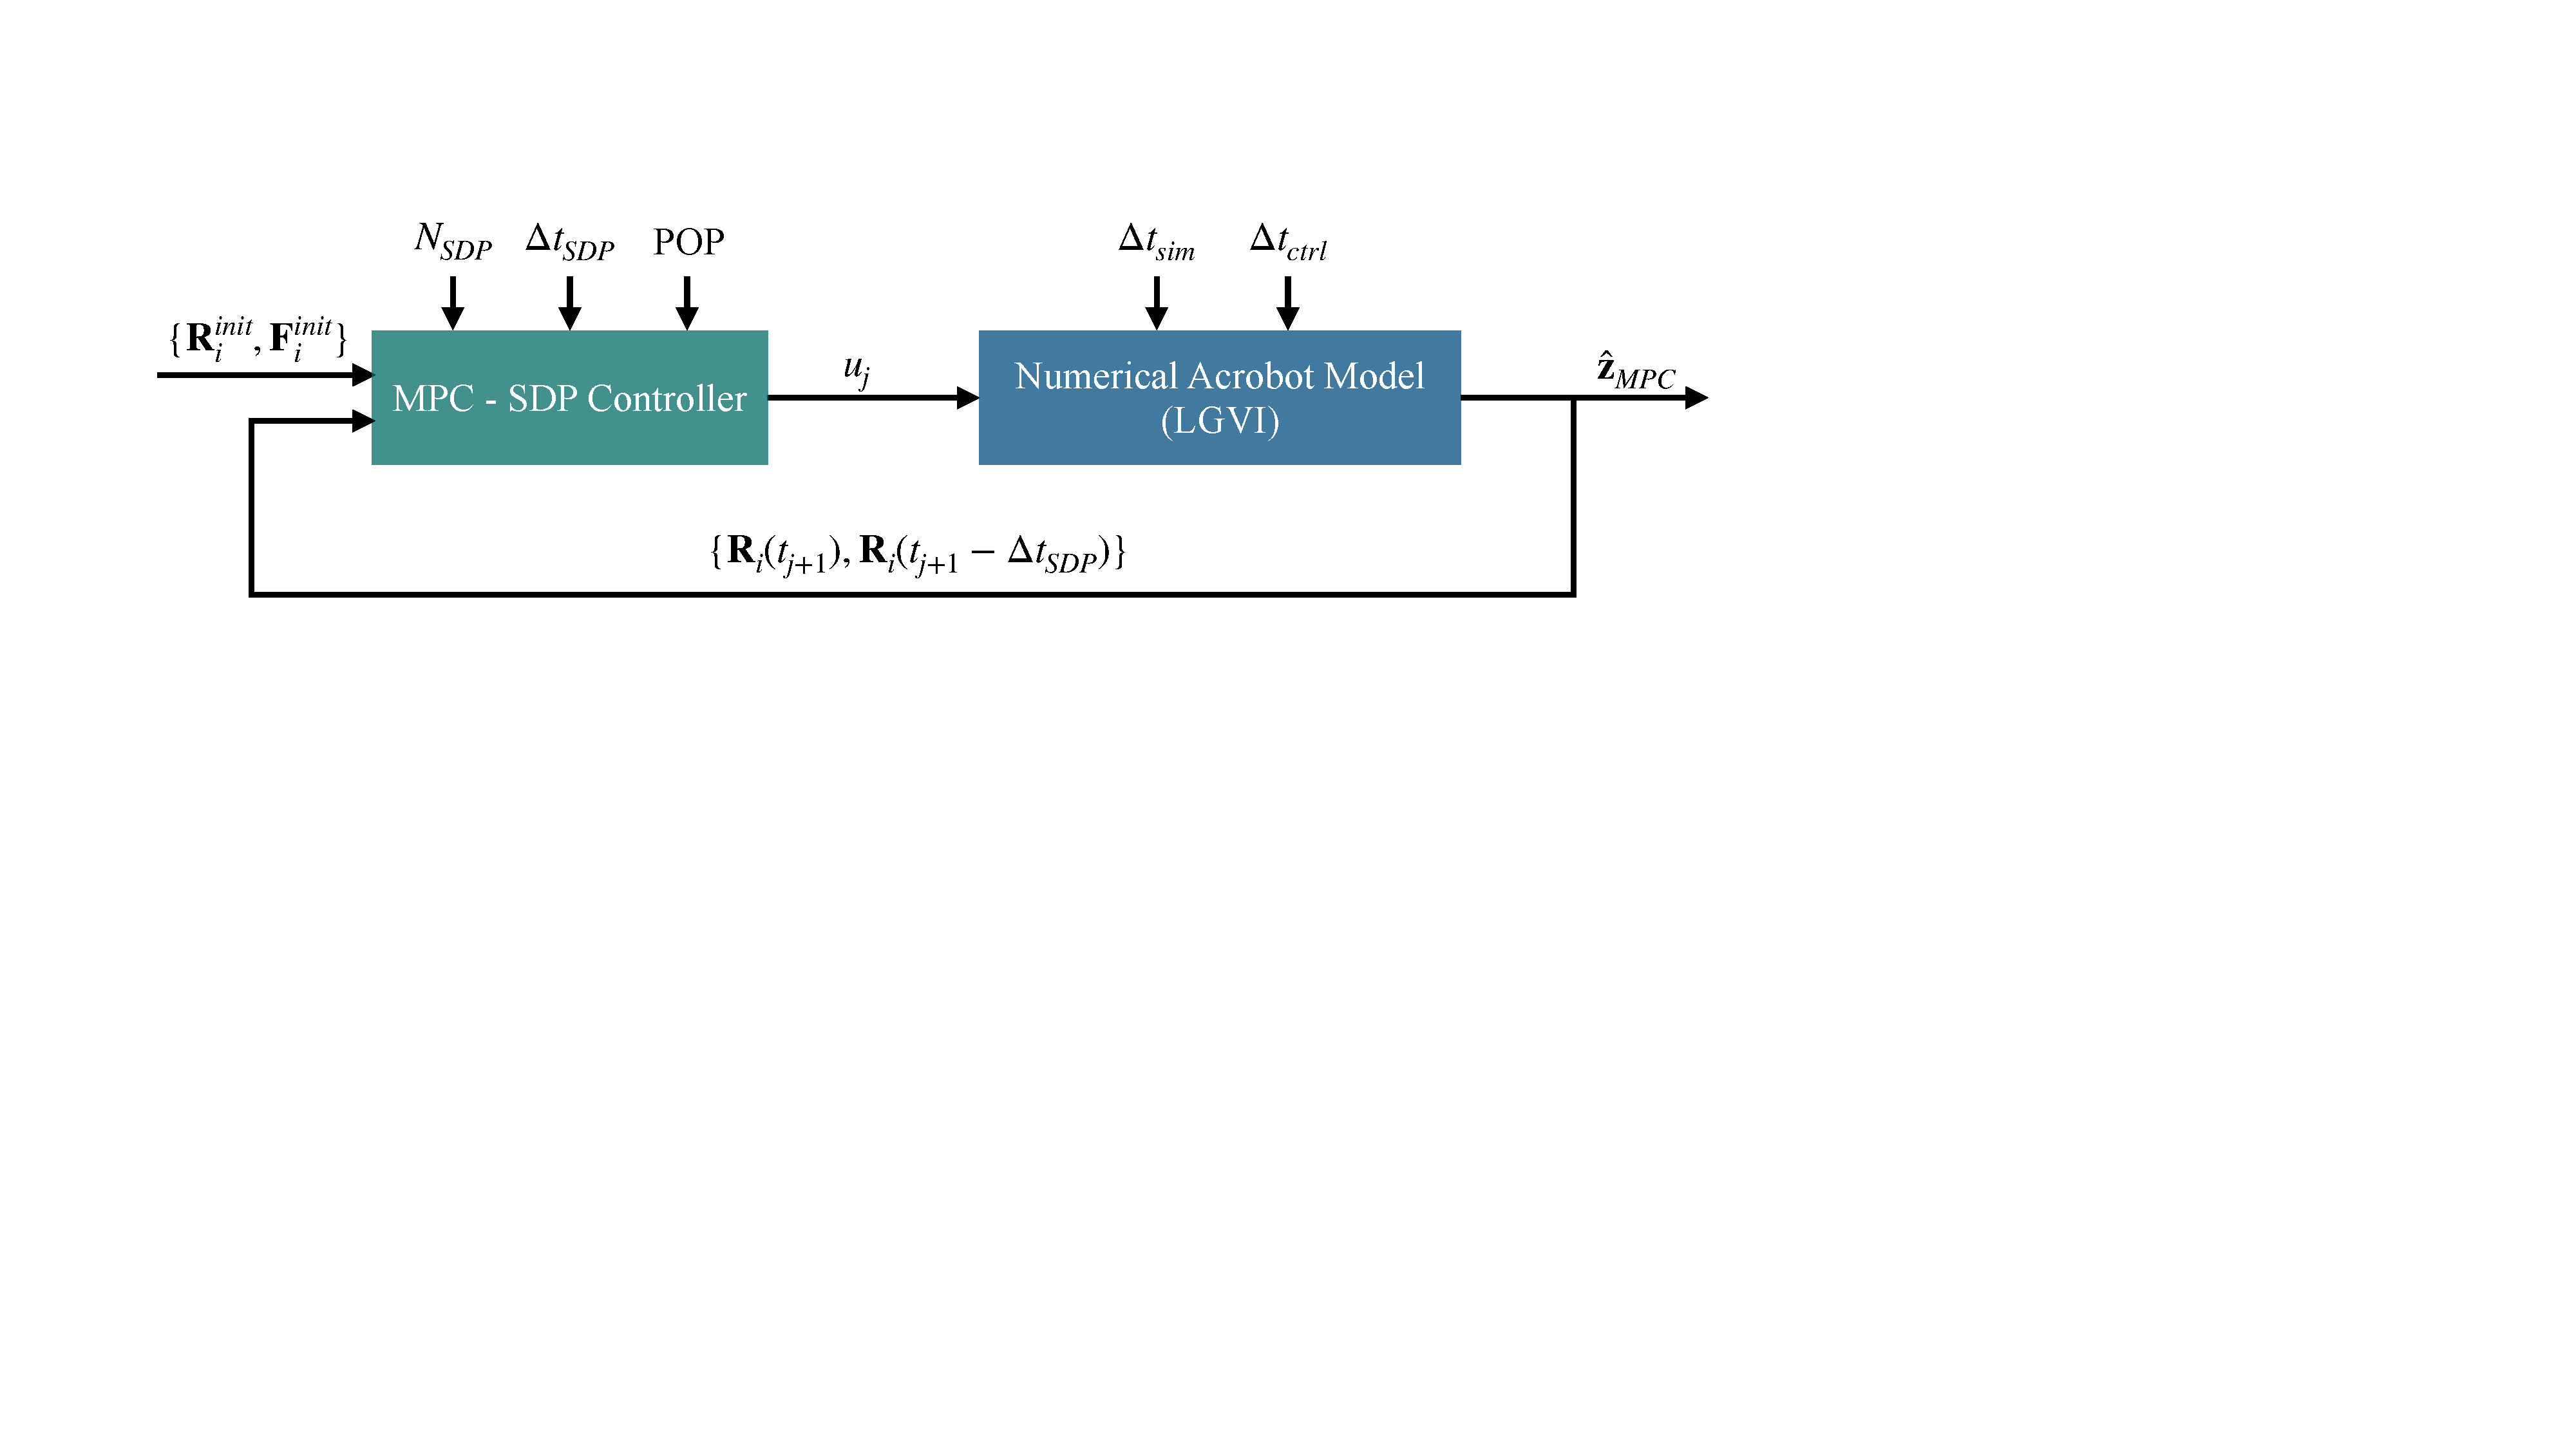
\includegraphics[width=\textwidth]{pics/Optimization/Acrobot/MPC_SDP_Loop.pdf}
    \caption{SDP-based model predictive control loop for the reduced Acrobot.}
    \label{fig:acrobot_sdp_mpc_loop}
\end{figure}

\paragraph{Receding-horizon}
In the following, \(j\in\mathbb{N}_0\) denotes the MPC iteration.
Therefore, the corresponding simulation time is
\begin{align}
t_j=j\Delta t_{\mathrm{ctrl}} 
\end{align}
In addition, \(k\mid j\) is the SDP prediction node \(k\)
of the problem solved at MPC iteration \(j\).
At every iteration, the second-order sparse Moment-SOS relaxation and
clique construction introduced in
Section~\ref{sec:trajectory_optimization_via_sdp_relaxation} are used.
Only the initial rotation data \(\bm{R}_{i,1\mid j}\), \(\bm{F}_{i,0\mid j}\), and
\(\bm{R}_{i,0\mid j}\) are updated from the simulated state, while the dynamics,
cost function, bounds, prediction horizon, and desired state remain unchanged.

For any two consecutive prediction nodes, the relative rotation satisfies
\begin{equation}
    \bm{F}_{i,k\mid j}
    =
    \bm{R}_{i,k\mid j}^{\top}\bm{R}_{i,k+1\mid j},
    \qquad
    \bm{R}_{i,k+1\mid j}
    =
    \bm{R}_{i,k\mid j}\bm{F}_{i,k\mid j}.
    \label{eq:acrobot_relative_rotation_general}
\end{equation}
At the boundary of each newly solved SDP problem, node \(k=1\) represents the
current simulated attitude at \(t_j\), whereas node \(k=0\) represents the
required history state one SDP interval earlier. Therefore, with
\(h=\Delta t_{\mathrm{SDP}}\), the updated boundary data are
\begin{equation}
\begin{aligned}
\bm{R}_{i,1\mid j}
&=\bm{R}_i(t_j),\\
\bm{F}_{i,0\mid j}
&=\bm{R}_i(t_j-\Delta t_{\mathrm{SDP}})^{\top}\bm{R}_i(t_j),\\
\bm{R}_{i,0\mid j}
&=\bm{R}_{i,1\mid j}\bm{F}_{i,0\mid j}^{\top},
\end{aligned}
\label{eq:acrobot_mpc_boundary_data}
\end{equation}
for links $i=1,2$.
The reconstruction \(\bm{F}_{i,0\mid j}=\bm{R}_i(t_j-\Delta t_{\mathrm{SDP}})^{\top}\bm{R}_i(t_j)\) ensures that the 
incoming relative rotation always spans exactly one SDP interval 
\(\Delta t_{\mathrm{SDP}}\). This is
important when the control interval \(\Delta t_{\mathrm{ctrl}}\) or the
simulation interval \(\Delta t_{\mathrm{sim}}\) differs from \(\Delta t_{\mathrm{SDP}}\).
However, during the first MPC iterations, the simulated state does not yet contain a full history
of past rotations for $\Delta t_{\mathrm{SDP}} > t_j$. Therefore, 
missing prehistory is completed using \(\bm{F}_i^{\mathrm{init}}=\bm{I}\),
simulating a stationary start.
\begin{align*}
\bm{R}_i(t)=\bm{R}_i(0)
\quad &\text{for } t<0, \\
\qquad
\bm{F}_{i,0\mid j}
=
\bm{R}_i(0)^\top \bm{R}_i(t_j)
\quad &\text{for }
0<t_j<\Delta t_{\mathrm{SDP}}.
\label{eq:initial_rotation_history}
\end{align*}

\paragraph{Control application}
After updating the boundary data at iteration \(j\), the reduced Acrobot POP
of Section~\ref{sec:trajectory_optimization_via_sdp_relaxation} is converted
into a second-order sparse SDP using SPOT and solved with MOSEK. Ordered
extraction of the degree-one moments provides the normalized first control
\(\bar u_{1\mid j}^{\star}\) from the solution vector 
\[\{\bar u_{1\mid j}^{\star}, \bar u_{2\mid j}^{\star},\dots, \bar u_{N_{\mathrm{SDP}}-1\mid j}^{\star}\}.\] The corresponding physical torque is
\begin{equation}
    u_j
    =
    u_{\max}\bar u_{1\mid j}^{\star}.
    \label{eq:acrobot_mpc_applied_control}
\end{equation}
Then, this first control $u_j$ is applied to the numerical Acrobot simulation 
of Section~\ref{subsec:evaluation_acrobot}, while the
remaining predicted control sequence is discarded. The control input
\(u_j\) is kept constant over the control interval 
$t_{j+1}=t_j+\Delta t_{\mathrm{ctrl}}$.
During this interval, the Acrobot is simulated using the reduced LGVI of
Section~\ref{subsection:discrete_Acrobot}. The simulated
trajectory at $j+1$ is then stored inside $\widehat{\bm{z}}_{\mathrm{MPC},j+1}$.
The resulting rotations and
rotation-steps are then used to construct the initial data for
the next SDP problem as described above. 

After the simulation interval, the rotation error \(e_{R,j}\) and the
relative-step rotation error \(e_{F,j}\) are evaluated. The latter is the
step-angle error calculated from the last fine simulation step and is measured
in degrees or radians, rather than degrees per second. The Acrobot is declared
stabilized if
\begin{equation}
    e_{R,j}\leq\varepsilon_R,
    \qquad
    e_{F,j}\leq\varepsilon_F
    \label{eq:acrobot_mpc_stabilization_condition}
\end{equation}
holds for \(n_{\mathrm{stable}}\) consecutive MPC updates. In this case, the
MPC loop terminates and the full simulated trajectory is 
saved inside $\widehat{\bm{z}}_{\mathrm{MPC},j+1}$. 
Otherwise, \(j\) is increased by one by the 
MPC-SDP controller, the initial data
is updated from the new simulated state, and the SDP is solved again. If the
SDP is infeasible or no finite first control can be extracted, the loop
terminates before another simulation interval.

\paragraph{Prediction horizon}
In summary, the MPC implementation uses
\begin{equation}
    \Delta t_{\mathrm{SDP}},
    \qquad
    \Delta t_{\mathrm{sim}},
    \qquad
    n_{\mathrm{sim}}
    =\frac{\Delta t_{\mathrm{ctrl}}}{\Delta t_{\mathrm{sim}}} \in \mathbb{N},
    \qquad
    T_{\mathrm{pred}}=(N_{\mathrm{SDP}}-1)\Delta t_{\mathrm{SDP}}.
    \label{eq:acrobot_mpc_time_scales}
\end{equation}
Here, \(\Delta t_{\mathrm{SDP}}\) is the discretization interval of the SDP prediction
model, \(\Delta t_{\mathrm{sim}}\) is the fine LGVI simulation step, and
\(\Delta t_{\mathrm{ctrl}}\) is the control interval between two MPC updates.
Consequently, the numerical plant performs \(n_{\mathrm{sim}}\) LGVI steps
before the SDP is solved again. The intervals \(\Delta t_{\mathrm{SDP}}\) and
\(\Delta t_{\mathrm{ctrl}}\) can differ from each other. If the two intervals are equal,
$\Delta t_{\mathrm{SDP}} = \Delta t_{\mathrm{ctrl}}$, one MPC
update corresponds to one predicted SDP interval.

Since node \(k=0\) contains the history state and node \(k=1\) the current
state, the \(N_{\mathrm{SDP}}-1\) future intervals give the prediction horizon
\(T_{\mathrm{pred}}=(N_{\mathrm{SDP}}-1)\Delta t_{\mathrm{SDP}}\).
Increasing \(N_{\mathrm{SDP}}\) 
provides a longer look-ahead for the swing-up but also increases the size
and solution time of the SDP. The complete decision logic of the SDP-based MPC loop is summarized in Figure~\ref{fig:acrobot_sdp_mpc_logic}.

\begin{figure}[!ht]
    \centering
    \resizebox{0.95\textwidth}{!}{%
        \begin{tikzpicture}[
    >=Stealth,
    font=\small,
    line/.style={draw, -{Stealth[length=2.2mm]}, line width=0.55pt},
    process/.style={
        draw,
        rectangle,
        align=center,
        minimum height=1.0cm,
        text width=4.6cm,
        inner xsep=3mm,
        inner ysep=2mm
    },
    wideprocess/.style={
        process,
        minimum height=1.15cm,
        text width=8.4cm
    },
    smallprocess/.style={
        process,
        minimum height=0.75cm,
        text width=4.2cm
    },
    decision/.style={
        draw,
        diamond,
        aspect=1.35,
        align=center,
        inner sep=1.5pt,
        text width=2.5cm
    },
    terminalbad/.style={
        process,
        draw=red,
        text width=3.7cm,
        minimum height=0.75cm,
        fill=red!3
    },
    terminalgood/.style={
        process,
        draw=green!65!black,
        text width=3.8cm,
        minimum height=0.75cm,
        fill=green!5
    }
]

\node[wideprocess] (update) at (4.25, -1.25)
    {Update SDP initial states\\[0.2em]
     \textcolor{red}{\eqref{eq:acrobot_mpc_boundary_data}}};

\node[draw, circle, minimum size=7mm, inner sep=0pt] (start) at ($(update.north)+(0,1.25cm)$) {};
\node[align=center, right=2mm of start] (initial) {$\bm{R}_i^{\mathrm{init}},\,\bm{F}_i^{\mathrm{init}}$};

\node[process, below left=1.05cm and 2.95cm of update.south] (solve)
    {Solve POP \textcolor{red}{\eqref{eq:controlled_acrobot_pop}} via SDP\\[0.2em]
     $\rightarrow$ extract $\bar u_{1\mid j}^{\star}$};

\node[terminalbad, below right=0.95cm and 0.15cm of solve.south east] (infeasible)
    {Terminate};

\node[smallprocess, below=1.95cm of solve, xshift=-1.2cm] (simulate)
    {Numerical simulation\\
     Acrobot LGVI \textcolor{red}{\eqref{eq:acrobot_full_del_shifted}}};

\node[smallprocess, below=0.8cm of simulate] (error)
    {Compute $e_{R,j+1},\,e_{\omega,j+1}$};

\node[decision, below right=0.9cm and 1.9cm of error.south] (terminal)
    {Check\\terminal\\condition\\
     \textcolor{red}{\eqref{eq:acrobot_mpc_stabilization_condition}}};

\node[terminalgood, below=0.9cm of terminal] (trajectory)
    {MPC trajectory $\bm{\hat{z}}_{\mathrm{A},\mathrm{mpc}}$};

\draw[line] (start) -- (update);

\draw[line]
    (update.west) -- (solve.north |- update.west) -- (solve.north);

\draw[line]
    (solve.south) -- ++(0,-0.55cm)
    -| node[pos=0.72, right, align=left] {Apply control $u_j$\\[-0.1em]
        \textcolor{red}{\eqref{eq:acrobot_mpc_applied_control}}}
    (simulate.north);

\draw[line]
    (solve.east) -- node[above] {infeasible} (infeasible.north |- solve.east)
    -- (infeasible.north);

\draw[line]
    (simulate.south) -- node[right] {$\bm{\hat{z}}_{\mathrm{A},\mathrm{MPC},j+1}$} (error.north);

\draw[line] (error.south) |- (terminal.west);

\draw[line]
    (terminal.south) -- node[right] {Yes} (trajectory.north);

\draw[line]
    (terminal.east) .. controls +(3.7cm,0.8cm) and +(1.6cm,-1.6cm) ..
    node[pos=0.31, anchor=west, xshift=10pt, fill=white, inner sep=1pt] {No: $j \leftarrow j+1$}
    (update.south east);

\end{tikzpicture}
%
    }
    \caption{Decision logic of the SDP-based model predictive control loop for the reduced Acrobot.}
    \label{fig:acrobot_sdp_mpc_logic}
\end{figure}

\chapter{Evaluation}
\label{chapter:evaluation}

This chapter evaluates the proposed modeling and optimization framework of Chapter \ref{chapter:certifiable_trajectory_optimization}.
Section~\ref{sec:numerical_simulation_results} first validates the derived LGVIs for the
3D pendulum and the Acrobot through numerical simulations. Sections~\ref{sec:3d_pendulum_optimization_results}
and~\ref{sec:acrobot_optimization_results} then assess the corresponding sparse Moment-SOS
trajectory optimization problems. Finally, Section~\ref{subsec:acrobot_sdp_mpc_results}
examines the closed-loop performance of the SDP-MPC formulation for the Acrobot.

\section{Numerical Simulation Results} 
\label{sec:numerical_simulation_results}

In this section, numerical simulations are conducted to evaluate 
the correctness of the derived discrete integrators for mechanical models on 
Lie groups. In particular, the structure-preserving properties of the variational 
discretizations derived in Section~\ref{sec:properties_discrete_lagrangian_flow} are examined. 
The analysis focuses 
especially on the preservation of the momentum map associated with the symmetry 
of the system, the evolution on the Lie-group configuration manifold, and the 
long-time behaviour of the total energy. This validation is important since 
discrete mechanical models obtained by variational integration provide a reliable 
basis for certifiable trajectory optimization. If the discrete flow violates 
the manifold structure or introduces artificial drift in conserved quantities such 
as momentum, the resulting optimization model becomes less faithful to the 
underlying mechanics \cite{Lee2008}. Additionally, for the 3D-pendulum, the
numerical simulations are compared with classical fourth-order Runge-Kutta methods and projected Runge-Kutta methods 
on \(SO(3)\) as reference integrators \cite{CELLEDONI2003421, Hairer2000}.
(see Table~\ref{tab:integrator_comparison}).

\begin{table}[h]
\centering
\caption{Comparison of the considered integration methods properties.}
\label{tab:integrator_comparison}
\begin{tabular}{lcc}
\hline
\textbf{Method} & \textbf{Symplectic} & \textbf{Manifold Preserving} \\
\hline
Variational Integrator & \cmark & \cmark \\
RK4 & \xmark & \xmark \\
Projected RK4 & \xmark & \cmark \\
\hline
\end{tabular}
\end{table}

\paragraph{Runge--Kutta 4th order}
As a baseline integrator, the classical explicit fourth-order Runge-Kutta (RK4) method is applied to the continuous rigid-body equations written as a first-order system $(\dot{\bm{R}},\dot{\bm{\omega}}) = \bm{f}(\bm{R},\bm{\omega})$. For a system of the form
\begin{align}
    \dot{\bm{y}} = \bm{f}(\bm{y}),
\end{align}
the classical RK4 scheme computes the four stage values
\begin{subequations}\label{eq:rk4_stages}
\begin{align}
    (\bm{k}_1^{R}, \bm{k}_1^{\omega}) &= \bm{f}(\bm{R}_n, \bm{\omega}_n), \\
    (\bm{k}_2^{R}, \bm{k}_2^{\omega}) &= \bm{f}\!\left(\bm{R}_n+\frac{h}{2}\bm{k}_1^{R},\bm{\omega}_n+\frac{h}{2}\bm{k}_1^{\omega}\right), \\
    (\bm{k}_3^{R}, \bm{k}_3^{\omega}) &= \bm{f}\!\left(\bm{R}_n+\frac{h}{2}\bm{k}_2^{R},\bm{\omega}_n+\frac{h}{2}\bm{k}_2^{\omega}\right), \\
   (\bm{k}_4^{R}, \bm{k}_4^{\omega}) &= \bm{f}\!\left(\bm{R}_n+h\bm{k}_3^{R}, \bm{\omega}_n+h\bm{k}_3^{\omega}\right),
\end{align}
\end{subequations}
and updates the numerical solution according to
\begin{subequations}\label{eq:rk4_update}
\begin{align}
    \bm{R}_{n+1}
    &=
    \bm{R}_n
    +
    \frac{h}{6}
    \left(
    \bm{k}_1^{R} + 2\bm{k}_2^{R} + 2\bm{k}_3^{R} + \bm{k}_4^{R}
    \right), \\
    \bm{\omega}_{n+1}
    &=
    \bm{\omega}_n
    +
    \frac{h}{6}
    \left(
    \bm{k}_1^{\omega} + 2\bm{k}_2^{\omega} + 2\bm{k}_3^{\omega} + \bm{k}_4^{\omega}
    \right),
\end{align}
\end{subequations}
for each discrete-time step $n$ \cite{butcher2016numerical}.

The explicit RK4 method does not preserve the orthogonality constraint \(\bm{R}^\top \bm{R}=\bm{I}\) and leaves the configuration manifold $SO(3)$, since the rotation matrix $\bm{R}_n$ is updated additively in the vector space of $\mathbb{R}^{3 \times 3}$ \cite{CELLEDONI2003421}.

\paragraph{RK4 projected to $SO(3)$}

The explicit RK4 method is combined with a projection of the updated discrete-time rotation matrix $\bm{R}_n$ onto $SO(3)$ to satisfy the orthogonality constraint
\[
SO(3)
=
\left\{
\bm{R}\in\mathbb{R}^{3\times 3}
\;\middle|\;
\bm{R}^\top \bm{R}=\bm{I}_3,\ 
\det(\bm{R})=1
\right\}.\]
After performing the RK4 step in $\mathbb{R}^{3 \times 3}$, the singular value decomposition of the obtained rotation matrix \(\widetilde{\bm{R}}_{n+1}\) is computed as
\begin{align}
    \widetilde{\bm{R}}_{n+1}=\bm{U}\bm{\Sigma}\bm{V}^{\top},
\end{align}
followed by a reconstruction of the updated rotation matrix
\begin{align}
    \bm{R}_{n+1}=\bm{U}\bm{V}^{\top},
\end{align}
which is projected onto $SO(3)$ \cite{YanaiTakeuchiTakane2011SVD}. Consequently, $\bm{R}_{n+1}$ satisfies the orthogonality constraint, while the angular velocity $\bm{\omega}_{n+1}$ remains unchanged in the vector space $\mathbb{R}^{3}$. However, this method does not inherit structure-preserving properties of the Lie group variational integrator, for example, symplecticity or momentum conservation \cite{CELLEDONI2003421}. 

\subsection{3D Pendulum}
\label{subsec:3d_pendulum_numercial_simulation}

For evaluating the preservation of the geometric properties of the previously 
defined 3D-pendulum (see Section \ref{sec:discrete_3D_pendulum}), 
numerical simulations are conducted for the unforced and controlled cases. The rigid body is modeled as a uniform solid cylinder of length $l=\SI{1}{\meter}$ and radius $r=\SI{5}{\cm}$, with its center of mass at $\frac{l}{2}$. Thereby, the physical parameters characterizing the configuration manifold are chosen as 
\begin{align}
    m &= \SI{1}{\kilogram}, &
    g &= \SI{9.81}{\meter\per\second\squared}, \\
    \bm{\rho}_c &=
    \begin{bmatrix}
        0 & 0 & 0.5
    \end{bmatrix}^\top \si{\meter}, &
    \bm{e}_3 &=
    \begin{bmatrix}
        0 & 0 & 1
    \end{bmatrix}^\top.
\end{align}
 The inertia matrix about the center of mass can be taken from the inertia table given in \cite{RITInertiaTable216}. The rotations about the $x$- and $y$-axes are about the central diameters, with $J_{11,com}=J_{22,com}= \frac{1}{12}m(3r^2 + l^2)$, while the rotation about the gravity-direction $z$-axis has $J_{33,com}=\frac{1}{2} mr^2$. The off-diagonal terms are equal to zero, because the body-fixed frame is aligned with the principal axes of the cylindrically symmetric body \cite{Lee2008}. Additionally, the inertia matrix about the pivot in body-frame is obtained by the parallel axis theorem of \cite{Benacquista2018ClassicalMechanics} given by
\begin{align}
    \bm{J}
    =
    \bm{J}_{\mathrm{com}}
    +
    m\left(
        \|\bm{\rho}_c\|^2\bm{I}
        -
        \bm{\rho}_c\bm{\rho}_c^{\top}
    \right).
\end{align}
After substituting the chosen values, the 3D-pendulum's inertia matrix is given by
\begin{align}
    \bm{J}
    &=
    \begin{bmatrix}
        0.33396 & 0 & 0 \\
        0 & 0.33396 & 0 \\
        0 & 0 & 0.00125
    \end{bmatrix}
    \si{\kilogram\meter\squared}.
\end{align}
Given \eqref{eq:non-standard_inertia}, the non-standard inertia matrix is calculated as
\begin{align}
    \bm{J}_d
    &=
    \begin{bmatrix}
        0.000625 & 0 & 0 \\
        0 & 0.000625 & 0 \\
        0 & 0 & 0.333333
    \end{bmatrix}
    \si{\kilogram\meter\squared}.
\end{align}
Using the introduced computational approach of Section \ref{sec:discrete_computational_approach}, the derived discrete-time implicit Hamilton equations
of the unforced \eqref{eq:discrete_3D_pendulum_hamilton} and controlled \eqref{eq:forced_3D_pendulum_hamilton} 3D-pendulum are converted to an equivalent vector equation in $\mathbb{R}^3$ using the Cayley transformation. From \cite{ColomboJimenez2012SO3_Cayley}, the corresponding nonlinear vector equation $\bm{0} = \bm{A}(\bm{f})$ of the 3D-pendulum is taken as
\begin{equation}\label{eq:simulation_3D_pendulum_vector_equation}
    \bm{0} = \bm{a}+\bm{a} \times \bm{f} + \bm{f}(\bm{a}^\top \bm{f})-2 \bm{J} \bm{f} = \bm{A}(\bm{f}),
\end{equation}
with $\bm{a}= h (\bm{\Pi}_k + \frac{h}{2} \bm{\tau}_{g,k})$. Additionally, \cite{ColomboJimenez2012SO3_Cayley} defines its Jacobian $\nabla \bm{A}\!\left(\bm{f}\right)$ as
\begin{align}\label{eq:Caley_Jacobian}
\nabla \bm{A}(\bm{f})
=
\hat{\bm{a}}
+
(\bm{a}^{\top}\bm{f})\bm{I}
+
\bm{f}\bm{a}^{\top}
-
2\bm{J}.
\end{align}
The tolerance for the Newton iteration is defined by $\left\lVert \bm{f}^{(i+1)} - \bm{f}^{(i)} \right\rVert < 10^{-12}$. The initial conditions are taken from \cite{Lee2008} 
\begin{align}
\bm{f}^0 &= (2 \bm{J} - \hat{\bm{a}})^{-1}\bm{a},&
    \bm{R}_0 &= \bm{I}, &
    \bm{\omega}_0 &=
    \begin{bmatrix}
        4.14 & 4.14 & 4.14
    \end{bmatrix}^{\top}\si{\radian\per\second},
\end{align} where $\bm{f}^0$ is the linearized solution of
\eqref{eq:simulation_3D_pendulum_vector_equation}.
In the following, the numerical simulation is plotted against time $t_k = kh$. 
The corresponding implementation is documented in the GitHub repository \cite{Elshani2026CTO_GitHub}.

\subsubsection{Unforced 3D-Pendulum}

\begin{figure}[t]
    \centering
    \begin{minipage}{0.49\textwidth}
        \centering
        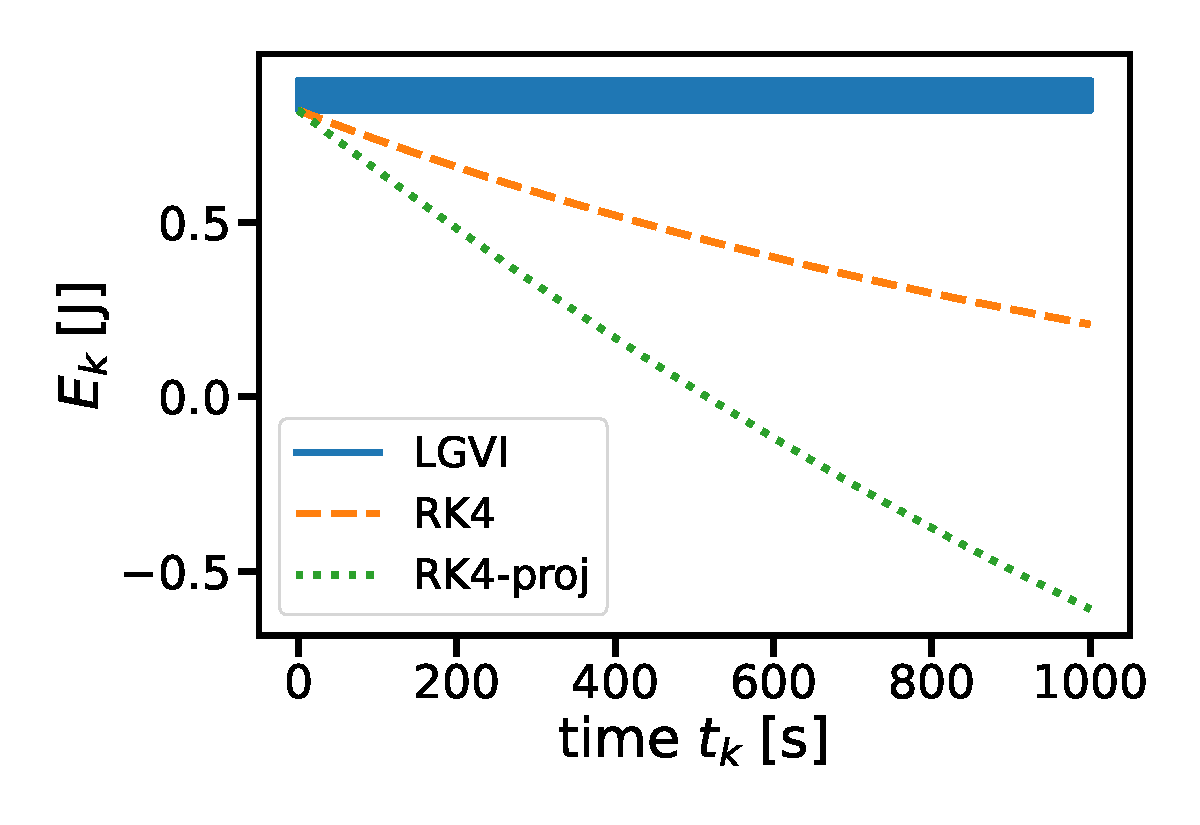
\includegraphics[width=\textwidth]{pics/Numerical_Simulation/Total_Energy.pdf}
        \caption*{(a) Total energy $E_k$.}
    \end{minipage}
    \hfill
    \begin{minipage}{0.49\textwidth}
        \centering
        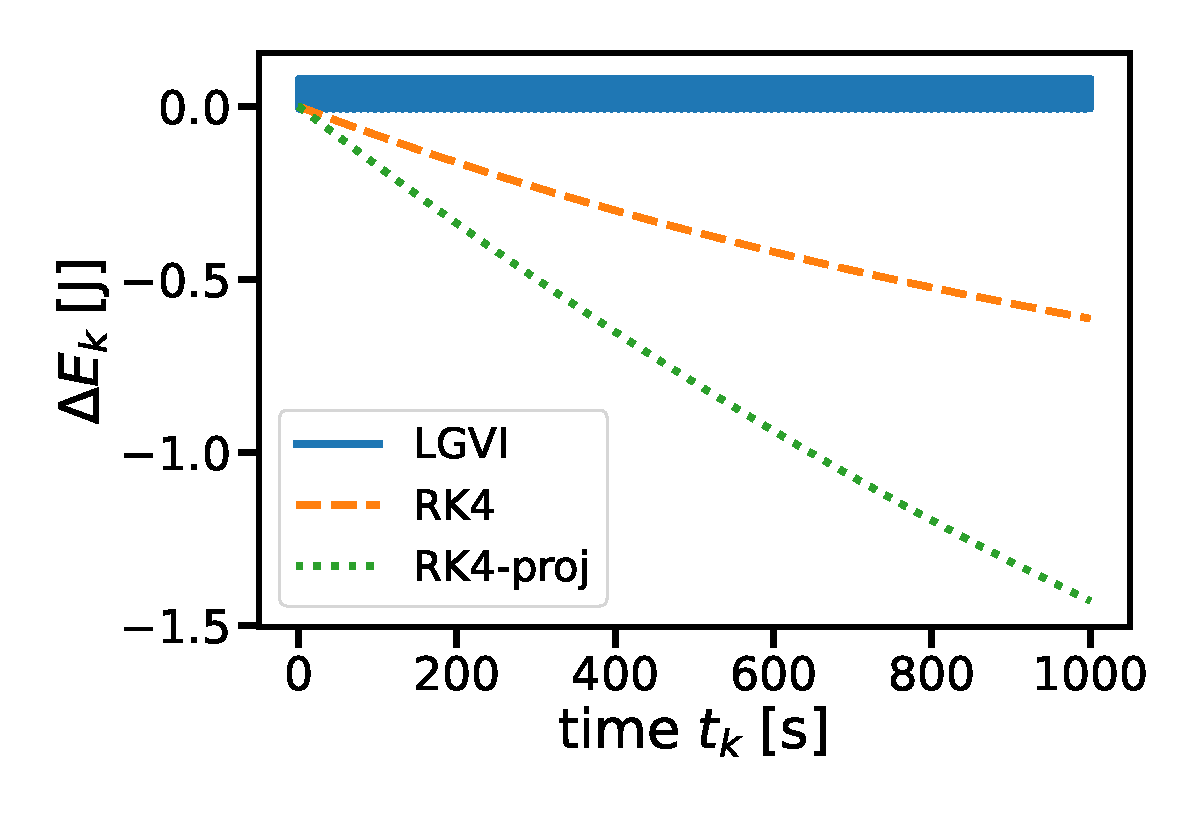
\includegraphics[width=\textwidth]{pics/Numerical_Simulation/Delta_E.pdf}
        \caption*{(b) Energy deviation $\Delta E_k$.}
    \end{minipage}

    \vspace{0.5em}

    \begin{minipage}{0.49\textwidth}
        \centering
        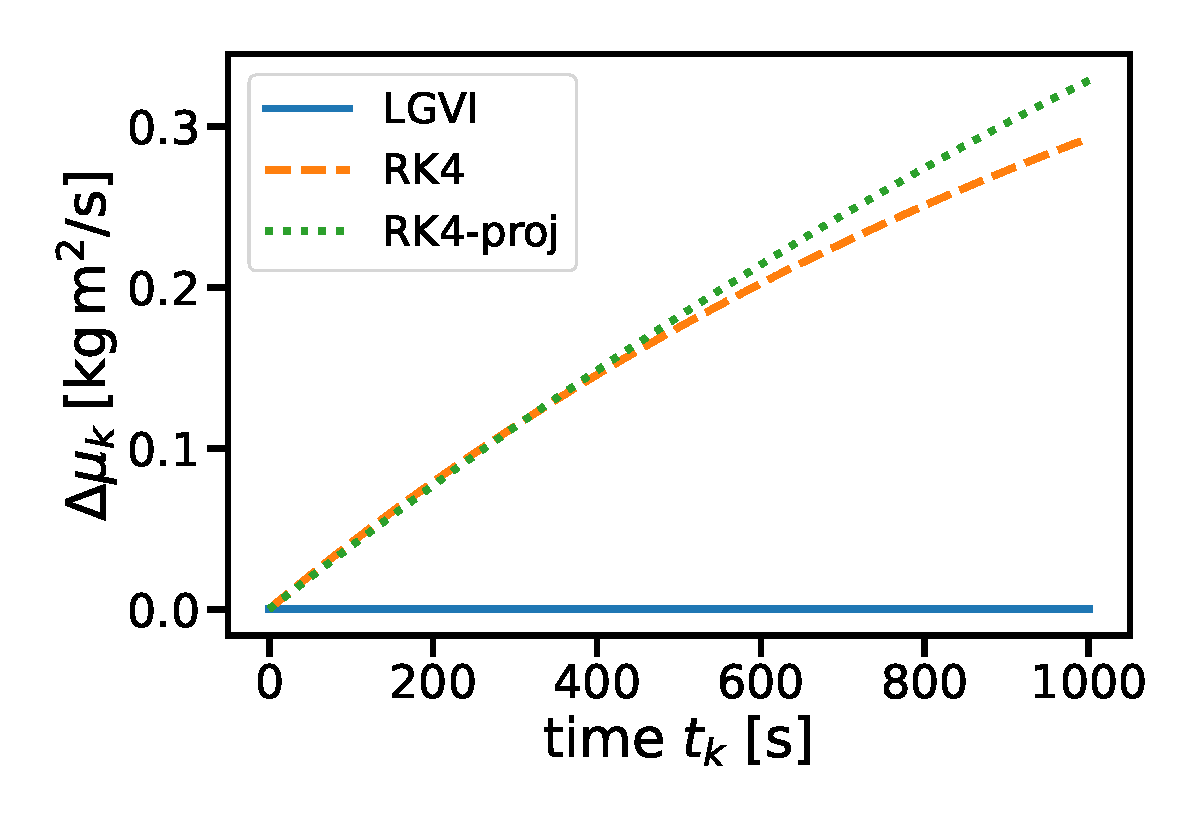
\includegraphics[width=\textwidth]{pics/Numerical_Simulation/Momentum_error.pdf}
        \caption*{(c) Momentum error $\Delta \mu_k$.}
    \end{minipage}
    \hfill
    \begin{minipage}{0.49\textwidth}
        \centering
        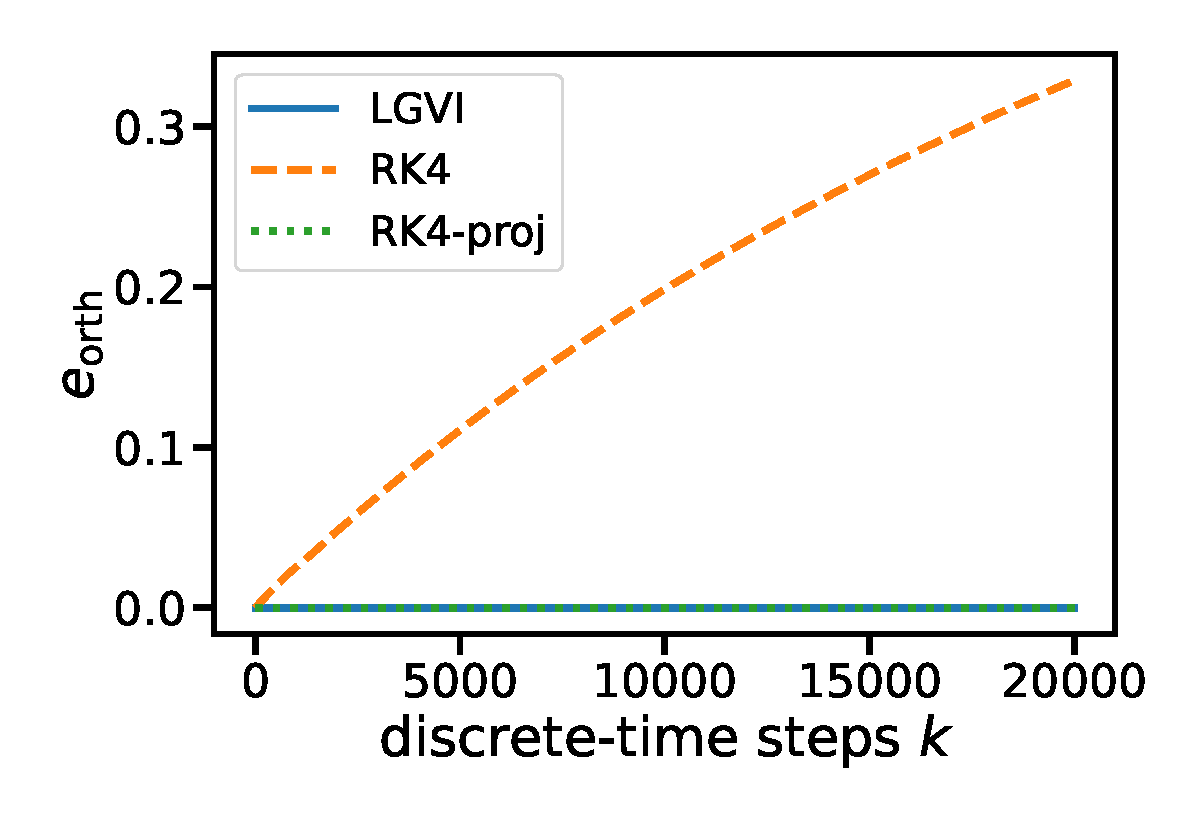
\includegraphics[width=\textwidth]{pics/Numerical_Simulation/Orthogonality_error.pdf}
        \caption*{(d) Orthogonality error $e_{orth}$.}
    \end{minipage}

    \caption{Comparison of the numerical preservation properties for the unforced $3$D pendulum.}
    \label{fig:simulation_results_3d_pendulum}
\end{figure}

The results of the numerical simulation for the unforced case, with 
$\bm{u}_k=\bm{0}$, are shown in Fig.~\ref{fig:simulation_results_3d_pendulum}. 
The simulation is performed over $20000$ discrete-time steps with a step size of 
$h=\SI{0.05}{\second}$. Thereby, the accuracy of the different integrator methods given in Table \ref{tab:integrator_comparison} is compared by plotting the corresponding total energy
\[
 E_k
    =
    \frac{1}{2}\bm{\omega}_k^{\top}\bm{J}\bm{\omega}_k
    -
    mg\,\bm{e}_3^{\top}\bm{R}_k\bm{\rho}_c,
\]
and its deviation $\Delta E_k = E_k - E_0$, the angular momentum error along the gravity direction
\[
\Delta \mu_k= \bm{e}_3^{\top}\bm{R}_k\bm{\Pi}_k - \bm{e}_3^{\top}\bm{R}_0\bm{\Pi}_0,
\]
defined in \cite{Lee2008}, and the orthogonality error 
\[
e_{\mathrm{orth},k} = \left\|\bm{I}-\bm{R}_k^{\top}\bm{R}_k\right\|_F.
\]

The total energy (see Fig. \ref{fig:simulation_results_3d_pendulum} (a)) and the corresponding energy deviation (see Fig. \ref{fig:simulation_results_3d_pendulum} (b)) illustrate the energy-preserving behavior of the Lie Group Variational Integrator (LGVI) over a long-time discrete flow. The energy remains close to the reference level with only small bounded oscillations because the symplectic method exactly solves a perturbed Hamiltonian \cite{Hairer1994}. However, RK4 and projected RK4 display a clear drift of the energy away from its true value, which remains constant for this unforced model.

Moreover, the momentum error (see Fig. \ref{fig:simulation_results_3d_pendulum} (c)) confirms that the LGVI method preserves the momentum, as validated for continuous time in \ref{sec:continuous_3D_pendulum_momentum_validation}. The computational results for RK4 and its projection onto $SO(3)$ show that these methods drift from the initial momentum value because they do not preserve the total angular momentum \cite{Lee2008}. In particular, projected RK4 has a larger discrepancy because it enforces $\bm{R}^\top\bm{R} = \bm{I}$ while leaving the angular velocity $\bm{\omega}$ unchanged, which influences the momentum.

Lastly, the orthogonality error highlights that the LGVI preserves the structure of the Lie group configuration manifold, as depicted in Fig. \ref{fig:simulation_results_3d_pendulum} (d). A similar result is obtained for projected RK4, while classical explicit RK4 violates the orthogonality constraint. For RK4, $e_{orth}$ increases linearly with the number of simulation time steps.

Consequently, only the LGVI preserves the manifold structure together with the momentum and energy behaviour over a long-time horizon. Although RK4 can be projected onto the Lie group manifold $SO(3)$, it cannot preserve the momentum and exhibits long-term energy drift.

\subsubsection{Controlled 3D-Pendulum}

In the controlled case, the previously derived free dynamics of the 3D-pendulum
are extended by an external body-fixed control moment. Following the control
structure defined in \eqref{eq:external_control_moment_3D_pendulum}, the time-dependent control parameter is chosen as
\begin{align}
    \label{eq:controlled_3d_pendulum_input_parameter}
    \bm{u}_p(t)
    =
    \begin{bmatrix}
        0.15\sin(0.5t) \\
        0.10\cos(0.25t) \\
        0
    \end{bmatrix}.
\end{align}
The corresponding discrete control input is obtained by evaluating the control law
at the discrete time nodes $\bm{u}_{p,k} =\bm{u}_p(t_k)$. Thus, the control input acts as a body-fixed external moment that is orthogonal to
the gravity direction expressed in the body frame, given by
$\bm{R}_k^{\top}\bm{e}_3$. Consequently, the control moment has no component
along this direction.

For the RK4 simulation, the continuous-time Hamilton equations \eqref{eq:continuous_3D_pendulum_hamilton} are used, 
with the control input $\bm{u}(t)$ added according to the Lagrange--d'Alembert principle of Section \ref{sec:discrete_forced_lagrangian}.
With the body angular momentum defined by $\bm{\Pi} = \bm{J}\bm{\omega}$,
the forced continuous-time equations of motion are written as
\begin{subequations}
\label{eq:controlled_3d_pendulum_continuous_RK4}
\begin{align}
    \dot{\bm{\Pi}}
    &=
    mg\,\bm{\rho}_c
    \times
    \bm{R}^{\top}\bm{e}_3
    -
    \bm{J}^{-1}\bm{\Pi}
    \times
    \bm{\Pi}
    +
    \bm{u}(t),
    \label{eq:controlled_3d_pendulum_continuous_momentum}
    \\
    \dot{\bm{R}}
    &=
    \bm{R}
    \left(
        \bm{J}^{-1}\bm{\Pi}
    \right)^{\wedge}.
    \label{eq:controlled_3d_pendulum_continuous_kinematics}
\end{align}
\end{subequations}
In contrast to the unforced case, the external input acts on the system.
Therefore, the total energy and the momentum map are no longer expected to be
conserved.

For the Lie group variational integrator, the forced discrete Hamilton equations
derived in \eqref{eq:forced_3D_pendulum_hamilton} are applied. The implicit
equation for the relative update $\bm{F}_k$ is again solved by using the Cayley
transformation. Compared to the unforced case, only the vector
$\bm{a}$ in \eqref{eq:simulation_3D_pendulum_vector_equation} changes due to
the additional control input. For the controlled dynamics, it is given by
\begin{align}
    \label{eq:controlled_3d_pendulum_cayley_a}
    \bm{a}
    =
    h
    \left(
        \bm{\Pi}_k
        +
        \frac{h}{2}
        \left(
            \bm{\tau}_{g,k}+\bm{u}_k
        \right)
    \right).
\end{align}
Therefore, the nonlinear vector equation \eqref{eq:simulation_3D_pendulum_vector_equation}
and its Jacobian \eqref{eq:Caley_Jacobian} are solved equivalently to the unforced simulation, with
the modified vector $\bm{a}$ including the control contribution. After computing
$\bm{f}_k$, the relative attitude update is obtained from the Cayley transformation
and the discrete-time states are propagated according to the forced LGVI. The corresponding implementation
is documented in the GitHub repository \cite{Elshani2026CTO_GitHub}.

The numerical simulation of the controlled 3D-pendulum compares the classical RK4 method with the forced
LGVI. Since the purpose of this experiment is to evaluate the behaviour of the
forced variational discretization under an external input, the projected RK4 method
is not considered in this comparison. The same physical parameters and initial
conditions as in the unforced case are used.

Fig.~\ref{fig:forced_3d_pendulum_results} shows the numerical results for the
controlled 3D-pendulum. The simulation is performed over $N=100000$ discrete-time
steps with step size $h=\SI{0.001}{\second}$. This shorter time interval is chosen
because the differences between the RK4 method and the forced LGVI already become
visible after a small number of time steps. During approximately the first eight
seconds, both methods show almost identical behaviour, which indicates that the
derived forced equations and their implementation are consistent. As the simulation
progresses, however, the trajectories begin to separate.

\begin{figure}[t]
    \centering
    \begin{minipage}{0.49\textwidth}
        \centering
        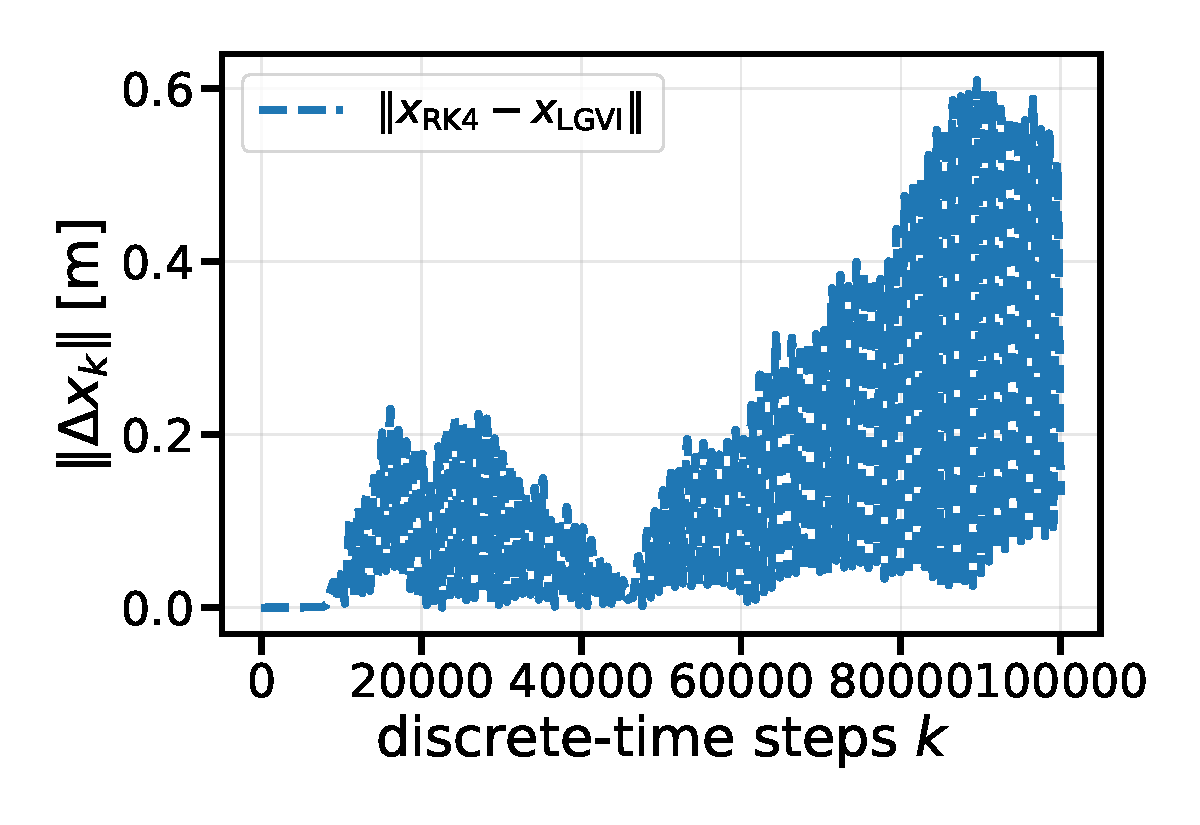
\includegraphics[width=\textwidth]{pics/Numerical_Simulation/Forced_3D_Pendulum_Trajectory.pdf}
        \caption*{(a) Position error norm $\|\Delta \bm{x}_k \||$.}
    \end{minipage}
    \hfill
    \begin{minipage}{0.49\textwidth}
        \centering
        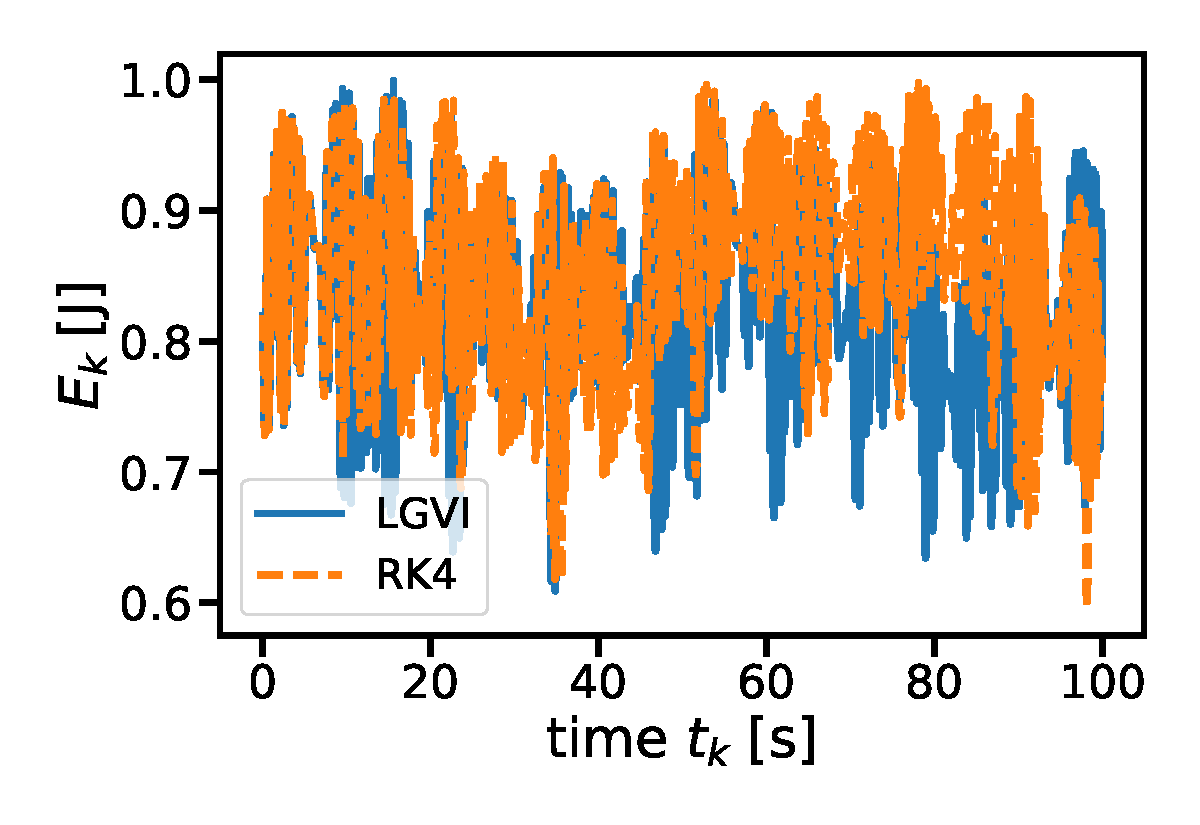
\includegraphics[width=\textwidth]{pics/Numerical_Simulation/Forced_3D_Pendulum_Ek.pdf}
        \caption*{(b) Total energy $E_k$.}
    \end{minipage}

    \vspace{0.5em}

    \begin{minipage}{0.49\textwidth}
        \centering
        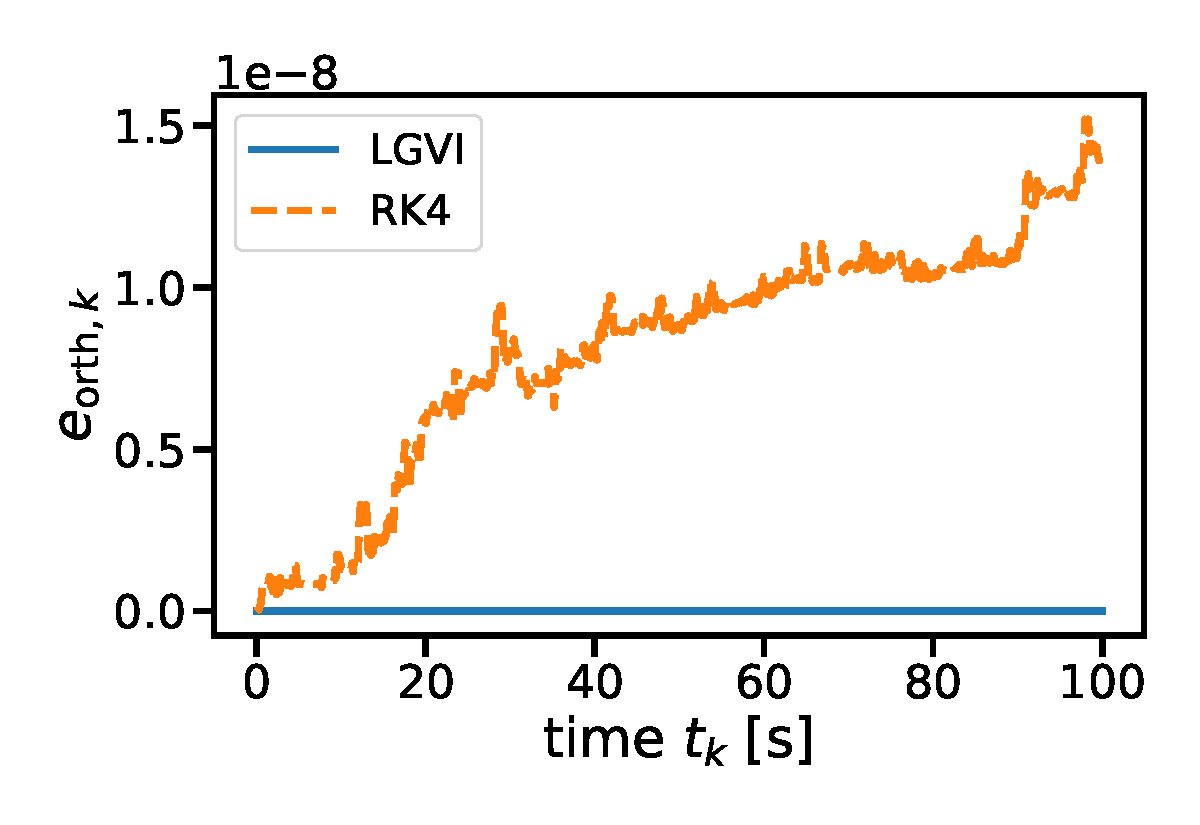
\includegraphics[width=\textwidth]{pics/Numerical_Simulation/Forced_3D_Pendulum_Orth_Error.pdf}
        \caption*{(c) Orthogonality error $e_{\mathrm{orth},k}$.}
    \end{minipage}
    \hfill
    \begin{minipage}{0.49\textwidth}
        \centering
        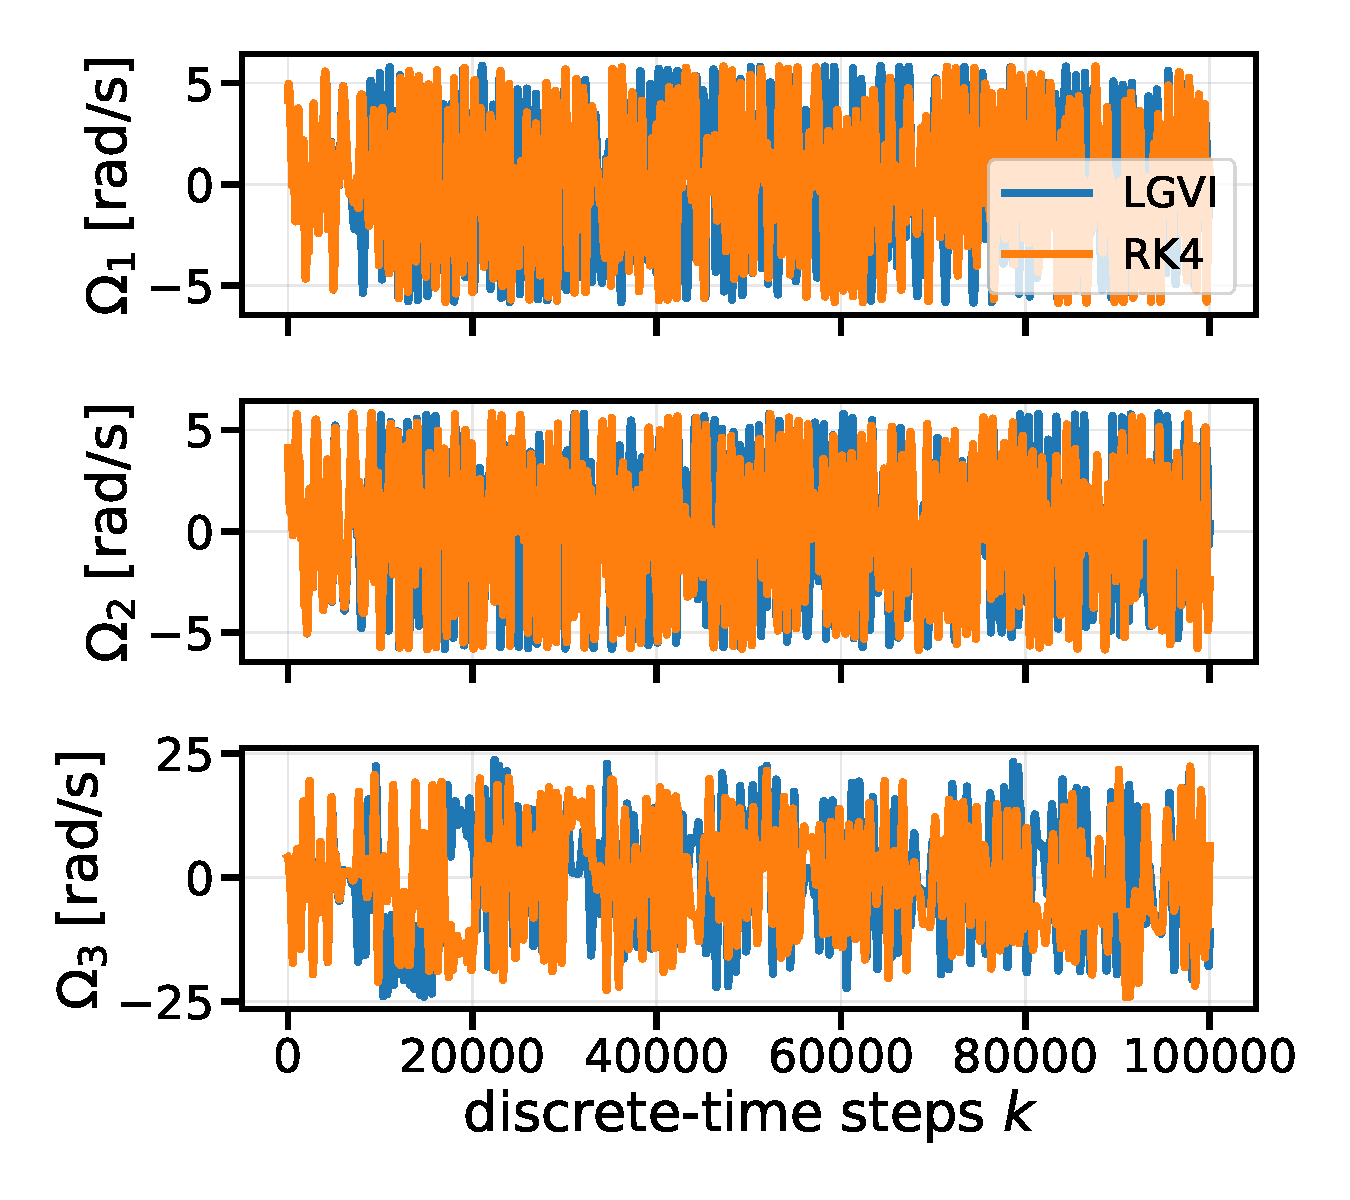
\includegraphics[width=\textwidth]{pics/Numerical_Simulation/Forced_3D_Pendulum_Omega.pdf}
        \caption*{(d) Angular velocity components $\bm{\omega}_k$.}
    \end{minipage}

    \caption{Comparison of the forced LGVI and RK4 simulation for the controlled $3$D pendulum.}
    \label{fig:forced_3d_pendulum_results}
\end{figure}

The position error in Fig.~\ref{fig:forced_3d_pendulum_results}~(a) is computed
from the center-of-mass position $\bm{x}_k=\bm{R}_k\bm{\rho}_c$,
as
\begin{align}
    \left\|\Delta \bm{x}_k\right\|_2
    =
    \left\|
        \bm{x}_{k,\mathrm{RK4}}
        -
        \bm{x}_{k,\mathrm{LGVI}}
    \right\|_2 .
\end{align}
The plot shows that the position error $\Delta \bm{x}_k$ is initially close to zero, but increases
over the simulation. Therefore, both methods reproduce the same short-time motion,
while their trajectories separate after a certain number of time steps. This behaviour is
expected for forced rigid-body dynamics, where small numerical
differences in the attitude $\bm{R}_k$ and momentum update $\bm{\Pi}_k$ can accumulate over time.

The total energy is shown in Fig.~\ref{fig:forced_3d_pendulum_results}~(b).
In contrast to the unforced case, the total mechanical energy is not expected to be
conserved, since the external input $\bm{u}_{p,k}$ acts on the system. It is observed that
the energetic behaviour of LGVI and RK4 under the same applied control
input follows a similar trend at the beginning, but small deviations
appear as the trajectories begin to separate, which is consistent with the position error.

The orthogonality error $e_{\mathrm{orth},k}$ is illustrated in Fig.~\ref{fig:forced_3d_pendulum_results}~(c).
Again, the plot confirms that the LGVI preserves the Lie group structure by staying on the manifold and updating the attitude through
$\bm{R}_{k+1}=\bm{R}_k\bm{F}_k$ with $\bm{F}_k\in SO(3)$. For RK4, the attitude is
updated additively in the surrounding vector space using the discrete update map \eqref{eq:rk4_update}. Over the short interval and due
to the small step size $h$, the orthogonality error remains small, but it is not preserved and increases over time.

Finally, Fig.~\ref{fig:forced_3d_pendulum_results}~(d) compares the angular
velocity components $\bm{\omega}_k$. In the discrete Hamiltonian formulation, the angular velocity
is recovered from the body angular momentum by
\begin{align}
    \hat{\bm{\omega}}_k
    =
    (\bm{J}^{-1}\bm{\Pi}_k)^\wedge,
\end{align}
discretizing and solving \eqref{eq:continuous_3D_pendulum_momentum} for $\hat{\bm{\omega}}_k$.
The angular velocity components of LGVI and RK4 are equal at the beginning of the
simulation, but begin to differ after a small number of steps. This confirms the
same behaviour observed in the position error $\Delta \bm{x}_k$ and the plotted energy $E_k$.
The 3D-Pendulum numerical simulation using external control inputs produces
consistent short-time dynamics of LGVI and RK4, while the numerical trajectories produced by the two methods separate as the
simulation continues.

\subsection{Acrobot}
\label{subsec:evaluation_acrobot}

To evaluate the preservation of the geometric properties of the previously defined Acrobot (see Section \ref{subsection:discrete_Acrobot}), 
numerical simulations are conducted for the unforced and controlled cases similar to those conducted for the 3D-pendulum 
in Section \ref{subsec:3d_pendulum_numercial_simulation}. 
In contrast to the 3D-pendulum, the Acrobot is a constrained multi-body system in maximal coordinates with the configuration 
\[
q_k =
\left(
\bm{x}_{1,k},
\bm{R}_{1,k},
\bm{x}_{2,k},
\bm{R}_{2,k}
\right)
\in
\left(\mathbb{R}^{2}\times SO(2)\right)^2 ,
\]
Therefore, the validation focuses not only on the preservation of the Lie-group structure of the attitude variables, but also on the preservation of the holonomic joint constraints $\bm{\phi}_0(q_k)$ and $\bm{\phi}_{12}(q_k)$. 
The physical parameters are chosen as two identical uniform rods with
\[
    m_1=m_2=1\,\mathrm{kg},
    \qquad
    l_1=l_2=1.0\,\mathrm{m},
    \qquad
    g=9.81\,\mathrm{m/s^2},
\]
and the center of mass of each link is located at $\frac{l_i}{2}$.
Since the maximal-coordinate formulation already represents the translational
motion of the link centers of mass, the rotational inertia is taken about the
corresponding center of mass. \cite{Benacquista2018ClassicalMechanics} defines
the rotational inertia of a uniform rod about its center of mass as
\[
    J_i^{\mathrm{com}}
    =
    \frac{1}{12}m_i l_i^2.
\]
By substituting the defined values of $m_i$ and $l_i$ into \eqref{eq:2D_nonstandard_inertia},
the non-standard inertia matrix of each link is given as
\[
    \bm{J}_{d,1}
    =
    \bm{J}_{d,2}
    =
    \begin{bmatrix}
        0.04167 & 0\\
        0 & 0.04167
    \end{bmatrix}
    \mathrm{kg\,m^2},
\]
The base point is fixed at
\[
    \bm{p}_0 =
    \begin{bmatrix}
        0 & 0
    \end{bmatrix}^{\top}.
\]
Using the body-fixed link convention from Section 4.3.1, the joint vectors are
\[
\bm{\rho}_{1,0}
=
\begin{bmatrix}
0 & 0.5
\end{bmatrix}^{\top}\mathrm{m},
\qquad
\bm{\rho}_{1,12}
=
\begin{bmatrix}
0 & -0.5
\end{bmatrix}^{\top}\mathrm{m},
\qquad
\bm{\rho}_{2,12}
=
\begin{bmatrix}
0 & 0.5
\end{bmatrix}^{\top}\mathrm{m},
\]
illustrated in Fig. \ref{fig:acrobot_maximal_coordinates}.

The implementation of the numerical simulation follows Section \ref{sec:discrete_computational_approach}. In contrast to \eqref{eq:simulation_3D_pendulum_vector_equation}, a unknown variable vector
\[
\bm{z}_{\mathrm{A},k}
=
\begin{bmatrix}
a_{1,k} & b_{1,k} & a_{2,k} & b_{2,k} &
\bm{\lambda}_{0,k}^{\top} &
\bm{\lambda}_{12,k}^{\top}
\end{bmatrix}^{\top},
\]
is defined. The nonlinear residual is written compactly as
\[
\bm{A}_{\mathrm{acro}}(\bm{z}_{\mathrm{A},k})
=
\begin{bmatrix}
\bm{A}_{T,k}\\
\bm{A}_{R,k}\\
a_{1,k}^2+b_{1,k}^2-1\\
a_{2,k}^2+b_{2,k}^2-1
\end{bmatrix}
=
\bm{0},
\]
where \(\bm{A}_{T,k}\) contains the translational dynamics \eqref{eq:acrobot_full_del_shifted_translation_1}-\eqref{eq:acrobot_full_del_shifted_translation_2} and \(\bm{A}_{R,k}\) contains the rotational dynamics \eqref{eq:acrobot_full_del_shifted_rotation_1}-\eqref{eq:acrobot_full_del_shifted_rotation_2}. After the nonlinear system has converged, the relative rotations \(\bm{F}_{i,k}\) are reconstructed and the link attitudes are updated by \(\bm{R}_{i,k+1}=\bm{R}_{i,k}\bm{F}_{i,k}\).

As in the controlled 3D-pendulum simulation, a classical fourth-order Runge--Kutta method is used as a reference integrator. The continuous-time Acrobot dynamics are implemented from the standard joint-coordinate equations given by \cite{tedrake_underactuated}. The resulting absolute link angles $\theta_{1,k}$ and $\theta_{2,k}$ are
mapped directly to the link rotations $\bm{R}_{1,k}$ and $\bm{R}_{2,k}$
using \eqref{eq:so2_rotation_matrix}. The complete implementation is documented in the GitHub repository \cite{Elshani2026CTO_GitHub}.

Additionally, the following metrics are used for the Acrobot simulation. 
The total mechanical energy is evaluated as
\[
E_k
=
\sum_{i=1}^{2}
\left(
    \frac{1}{2}\bm{v}_{i,k}^{\top}\bm{M}_i\bm{v}_{i,k}
    +
    \frac{1}{2}J_i^{\mathrm{com}}\omega_{i,k}^{2}
    -
    g \bm{e}_2^{\top}\bm{M}_i\bm{x}_{i,k}
\right).
\]
where $\bm{M}_i = m_i \bm{I}$ denotes the mass matrix of link $i$. The position difference between the LGVI trajectory and the reconstructed RK4 reference trajectory is computed by
\[
\left\|\Delta \bm{x}_k\right\|_2
=
\left\|
\bm{X}_{k,\mathrm{RK4}}
-
\bm{X}_{k,\mathrm{LGVI}}
\right\|_2,
\]
with $\bm{X}_k =
\begin{bmatrix}
\bm{x}_{1,k}^{\top} & \bm{x}_{2,k}^{\top}
\end{bmatrix}^{\top}$. The holonomic constraint residuals are evaluated separately as
$
\|\bm{\phi}_{0,k}\|_2,$
and
$\|\bm{\phi}_{12,k}\|_2,
$
where $\bm{\phi}_{0,k}$ and $\bm{\phi}_{12,k}$ are defined in \eqref{eq:acrobot_base_constraint} and \eqref{eq:acrobot_elbow_constraint}. Finally, the Lie-group preservation of both link attitudes is measured by
\[
e_{\mathrm{orth},i,k}
=
\left\|
\bm{I}_2 - \bm{R}_{i,k}^{\top}\bm{R}_{i,k}
\right\|_F,
\qquad
i\in{1,2}.
\]
In contrast to the 3D-pendulum, no momentum-map error is evaluated for the Acrobot, as the system does not possess the same rotational symmetry about the gravity direction as the 3D-pendulum.
For the unforced and controlled Acrobot simulations, both links start from the
identity attitude with the same absolute angular velocity,
\[
\bm{R}_{i,0}=\bm{I},
\qquad
\omega_{i,0}=4.14\,\si{\radian\per\second},
\qquad i\in\{1,2\}.
\]

\subsubsection{Unforced Acrobot}

The first Acrobot simulation considers the unforced case with $u_k=0$. The simulation is performed with the step size $ h=\SI{0.01}{\second}$ 
over the final time $ t_f=\SI{1000}{\second}$, which corresponds to $N=100000$ discrete-time steps.
\begin{figure}[t]
    \centering
    \begin{minipage}{0.49\textwidth}
        \centering
        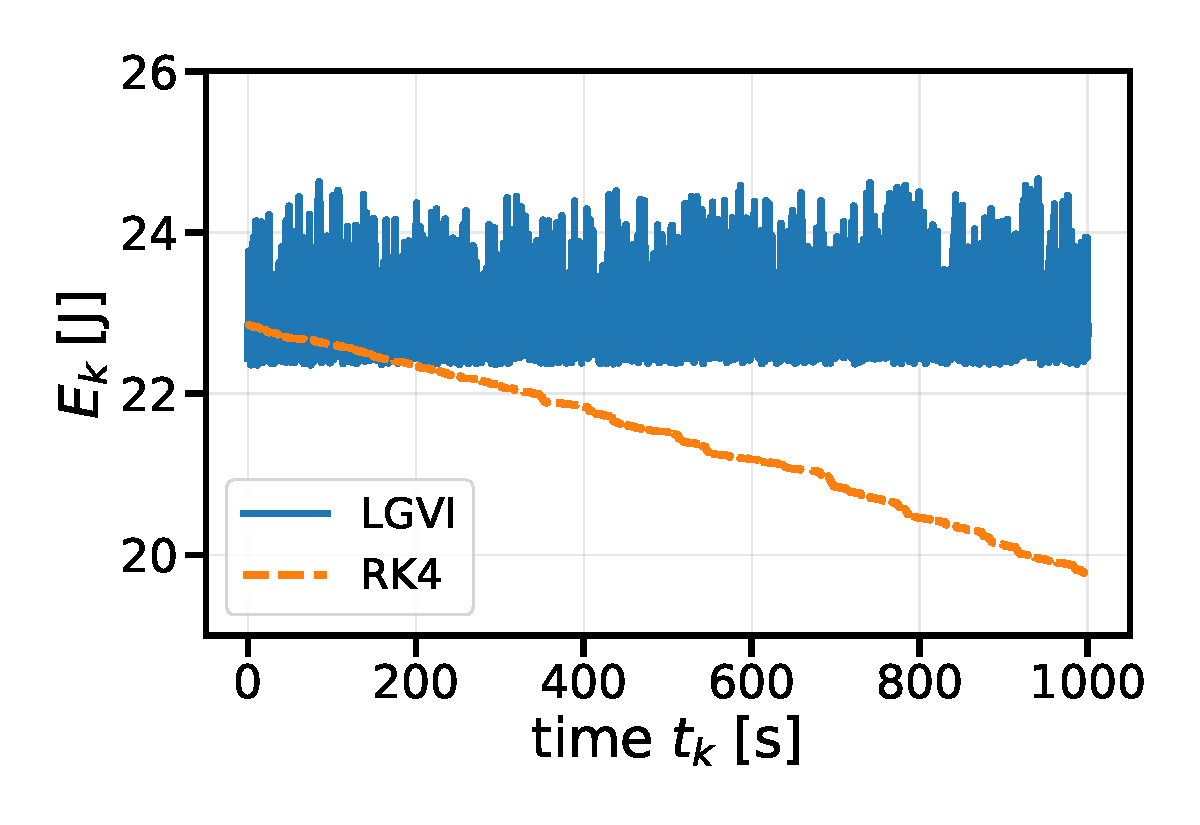
\includegraphics[width=\textwidth]{pics/Numerical_Simulation/Acrobot/acrobot_total_energy.pdf}
        \caption*{(a) Total energy $E_k$.}
    \end{minipage}
    \hfill
    \begin{minipage}{0.49\textwidth}
        \centering
        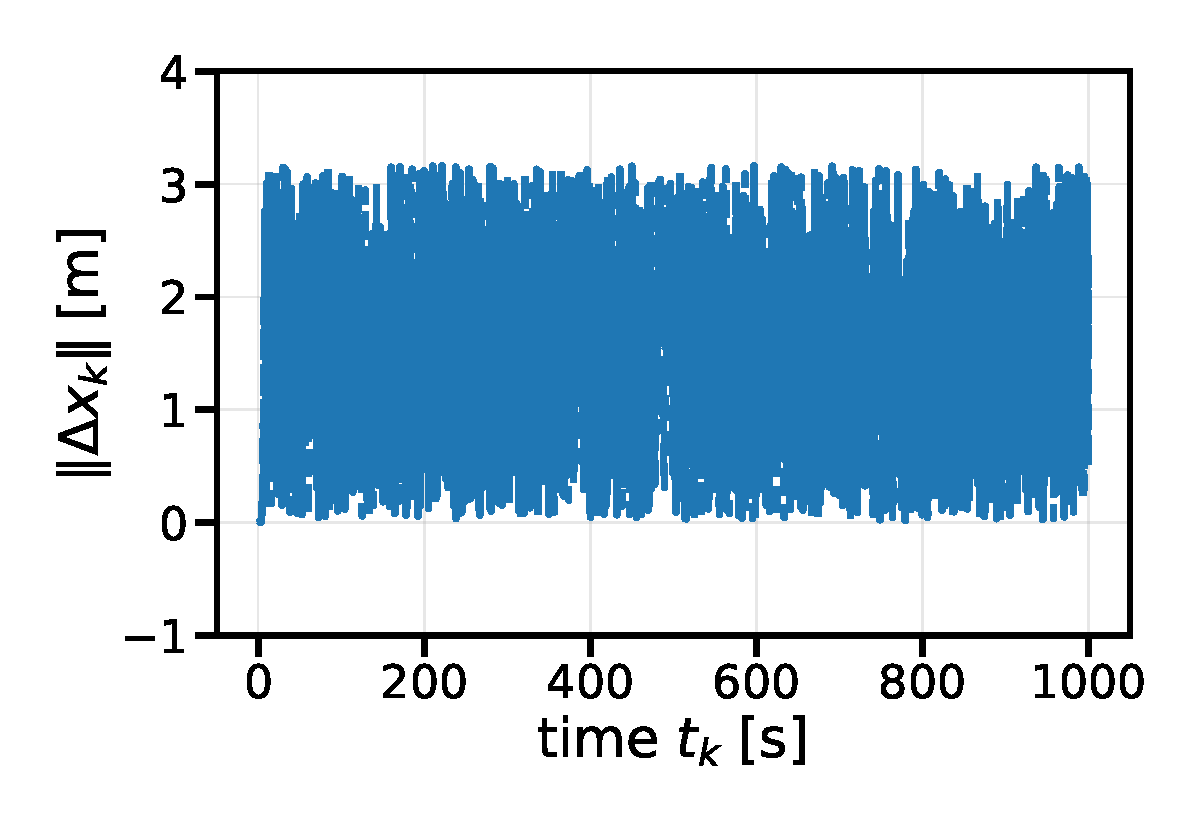
\includegraphics[width=\textwidth]{pics/Numerical_Simulation/Acrobot/acrobot_position_error_norm.pdf}
        \caption*{(b) Position error norm $\|\Delta \bm{x}_k \||$.}
    \end{minipage}

    \vspace{0.5em}

    \begin{minipage}{0.49\textwidth}
        \centering
        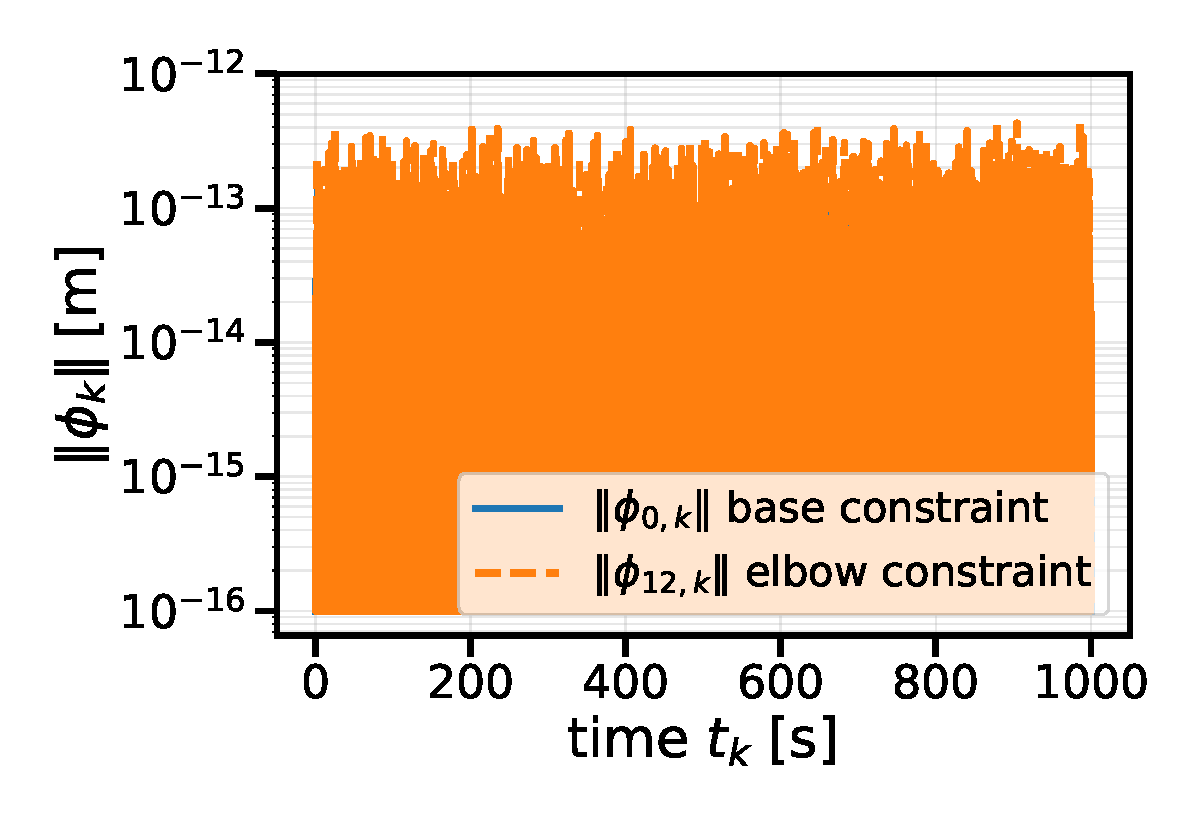
\includegraphics[width=\textwidth]{pics/Numerical_Simulation/Acrobot/acrobot_holonomic_constraint_residuals.pdf}
        \caption*{(c) Holonomic constraint residual $\bm{\phi}$.}
    \end{minipage}
    \hfill
    \begin{minipage}{0.49\textwidth}
        \centering
        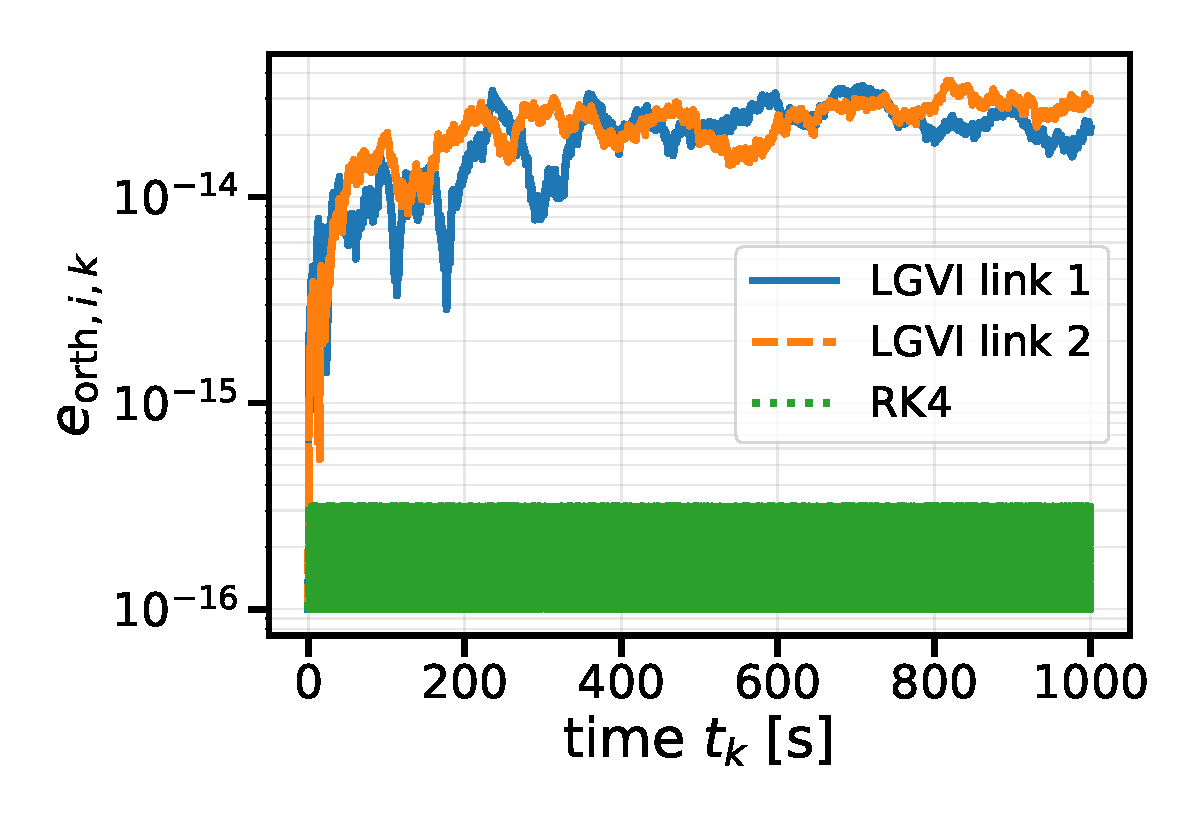
\includegraphics[width=\textwidth]{pics/Numerical_Simulation/Acrobot/acrobot_orthogonality_error.pdf}
        \caption*{(d) Orthogonality error $e_{orth}$.}
    \end{minipage}

    \caption{Comparison of the numerical preservation properties for the unforced Acrobot.}
    \label{fig:simulation_results_acrobot_unforced}
\end{figure}

The total energy $E_k$ is shown in Fig.\ref{fig:simulation_results_acrobot_unforced}(a). Since the system is unforced, the exact mechanical energy is expected to remain constant. The LGVI energy remains close to its initial value and shows bounded oscillations over the long-time horizon. This behaviour is consistent with the symplectic structure of variational integrators introduced in Section \ref{sec:properties_discrete_lagrangian_flow}. In contrast, the RK4 reference shows a visible drift of the energy over time. This agrees with the observation from the unforced 3D-pendulum simulation in Fig.\ref{fig:simulation_results_3d_pendulum}.

Fig.~\ref{fig:simulation_results_acrobot_unforced}(b) shows the position error norm
$\|\Delta \bm{x}_k\|$ between the LGVI trajectory and the reconstructed RK4
reference. It subsequently grows and oscillates over the long-time
horizon, reaching a maximum of approximately $\SI{3.16}{\meter}$. The deviation is reasoned, by
the numerical differences between the two
integrators LGVI and RK4.

The holonomic constraint residuals $\|\bm{\phi}_{0,k}\|_2$ and $\|\bm{\phi}_{12,k}\|_2$ are shown in Fig.\ref{fig:simulation_results_acrobot_unforced}(c). Both the base constraint residual $\|\bm{\phi}_{0,k}\|_2$ and the elbow constraint residual $\|\bm{\phi}_{12,k}\|_2$ remain close to machine precision over the complete simulation ($< 10^{-12}$). This confirms that the constrained LGVI in maximal-coordinates \eqref{eq:acrobot_full_del_shifted} enforces the fixed-base joint and the elbow joint at the position level.

Finally, Fig.\ref{fig:simulation_results_acrobot_unforced}(d) shows the orthogonality error $e_{orth,i,k}$ of both link rotations. The LGVI preserves the $SO(2)$ structure of both attitudes by the multiplicative update $\bm{R}_{i,k+1}=\bm{R}_{i,k}\bm{F}_{i,k}$ with $\bm{F}_{i,k}\in SO(2)$. The RK4 reference also remains very small, because it is integrated in relative coordinates and then reconstructed into rotation matrices. However, the LGVI shows a slightly larger error, which is caused by the finite tolerance of the Newton iteration used to compute the Cayley parameters. Nevertheless, the orthogonality error remains below $10^{-13}$ over the complete simulation.

Overall, the unforced Acrobot simulation confirms that the derived constrained LGVI preserves the geometric structure of the maximal-coordinate model. The link attitudes remain on $SO(2)$, the joint constraints remain satisfied, and the energy shows bounded long-time behaviour.

\subsubsection{Controlled Acrobot}

The Acrobot is actuated by a scalar torque at the elbow joint. As derived in \eqref{eq:acrobot_generalized_torque}, this torque is an internal joint torque acting between the two links.
The control input is chosen as the sinusoidal elbow torque
\[
u(t)=0.15\sin(0.7t)\,\si{\newton\meter}.
\]
The discrete input is obtained by evaluating the continuous input at the time nodes, $u_k=u(t_k)$. The forced simulation uses the same physical parameters and initial condition as the unforced case. The simulation is performed with
\[
h=\SI{0.001}{\second},
\qquad
t_f=\SI{100}{\second},
\]
corresponding to $N=100000$ discrete-time steps. The same metrics as in the unforced case are evaluated.

\begin{figure}[t]
    \centering
    \begin{minipage}{0.49\textwidth}
        \centering
        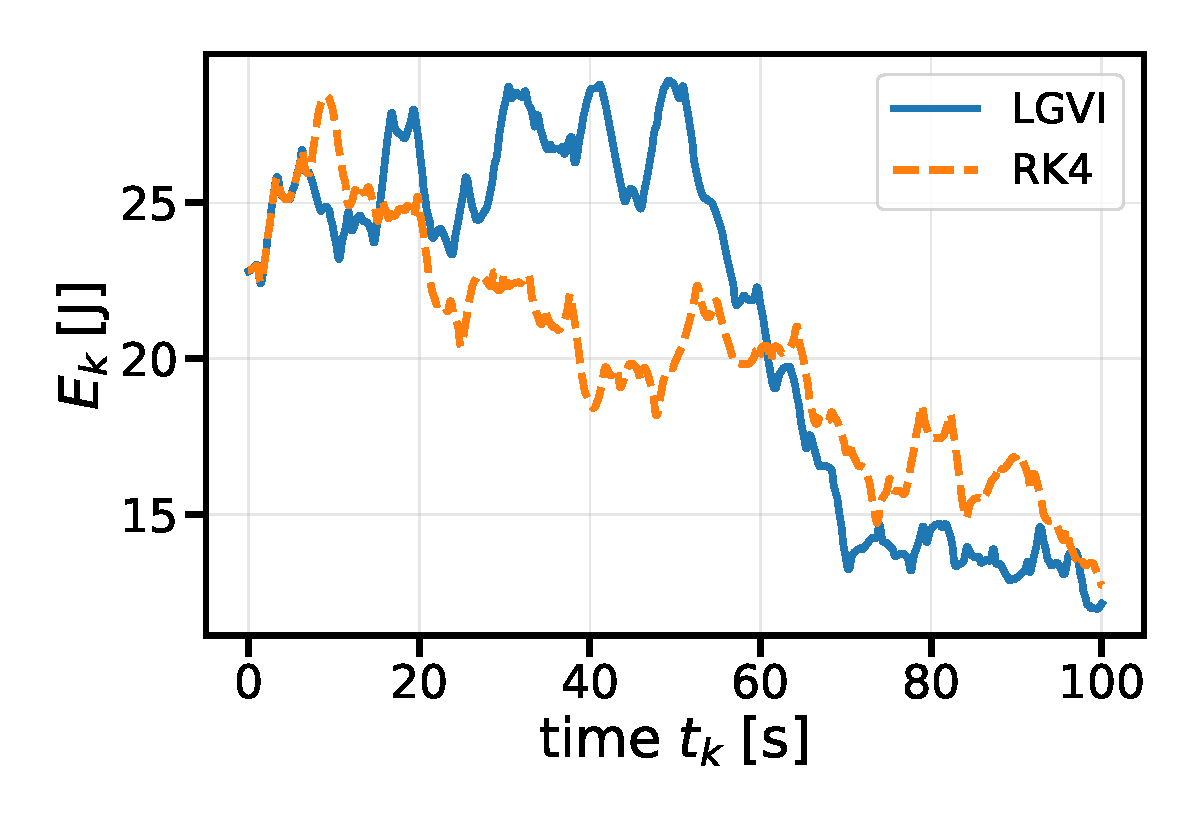
\includegraphics[width=\textwidth]{pics/Numerical_Simulation/Acrobot/forced_sine_total_energy.pdf}
        \caption*{(a) Total energy $E_k$.}
    \end{minipage}
    \hfill
    \begin{minipage}{0.49\textwidth}
        \centering
        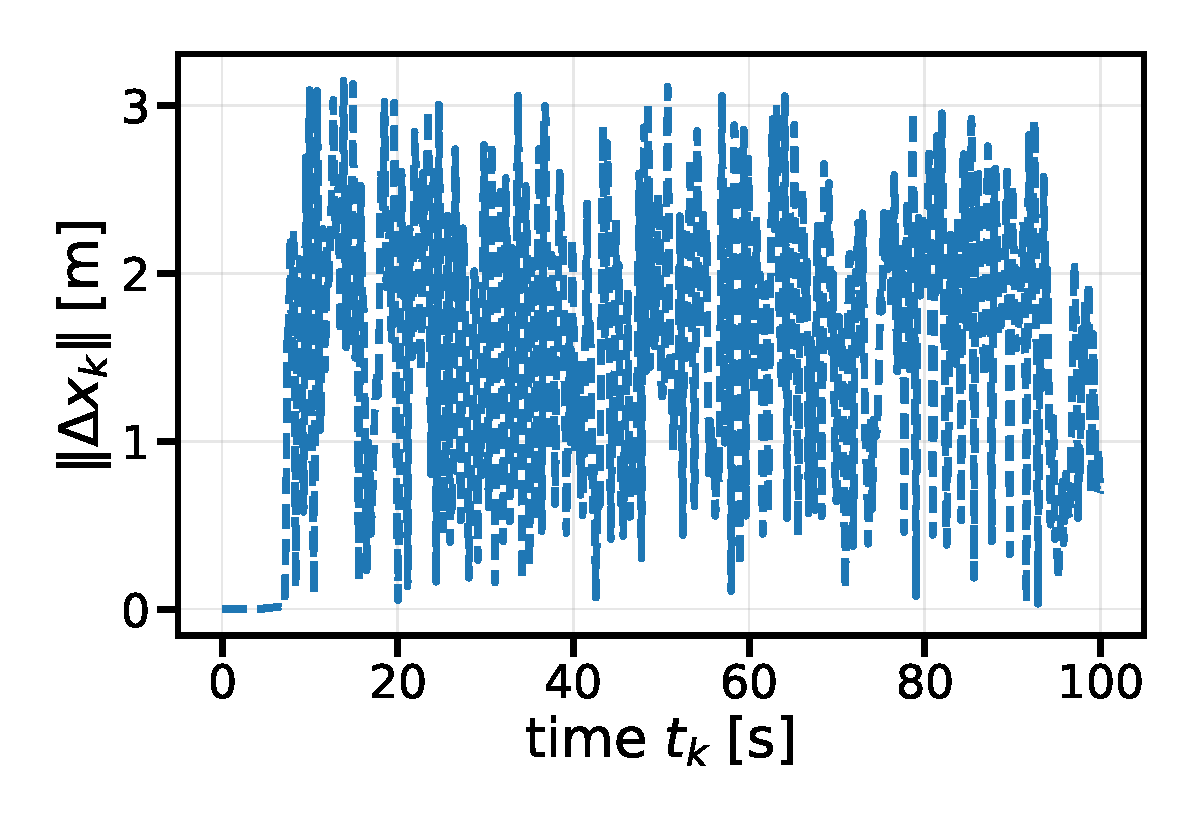
\includegraphics[width=\textwidth]{pics/Numerical_Simulation/Acrobot/forced_sine_position_error.pdf}
        \caption*{(b) Position error norm $\|\Delta \bm{x}_k \|$.}
    \end{minipage}

    \vspace{0.5em}

    \begin{minipage}{0.49\textwidth}
        \centering
        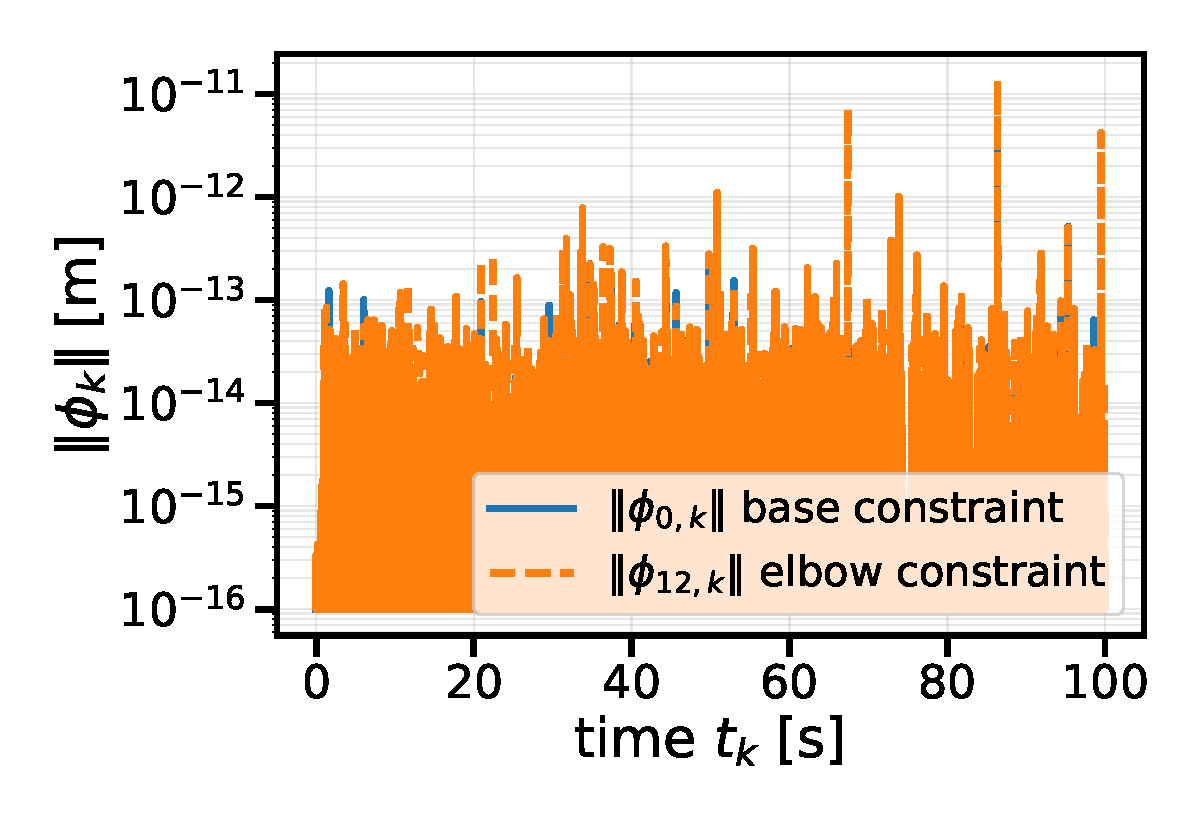
\includegraphics[width=\textwidth]{pics/Numerical_Simulation/Acrobot/forced_sine_constraint_residuals.pdf}
        \caption*{(c) Holonomic constraint residual $\bm{\phi}$.}
    \end{minipage}
    \hfill
    \begin{minipage}{0.49\textwidth}
        \centering
        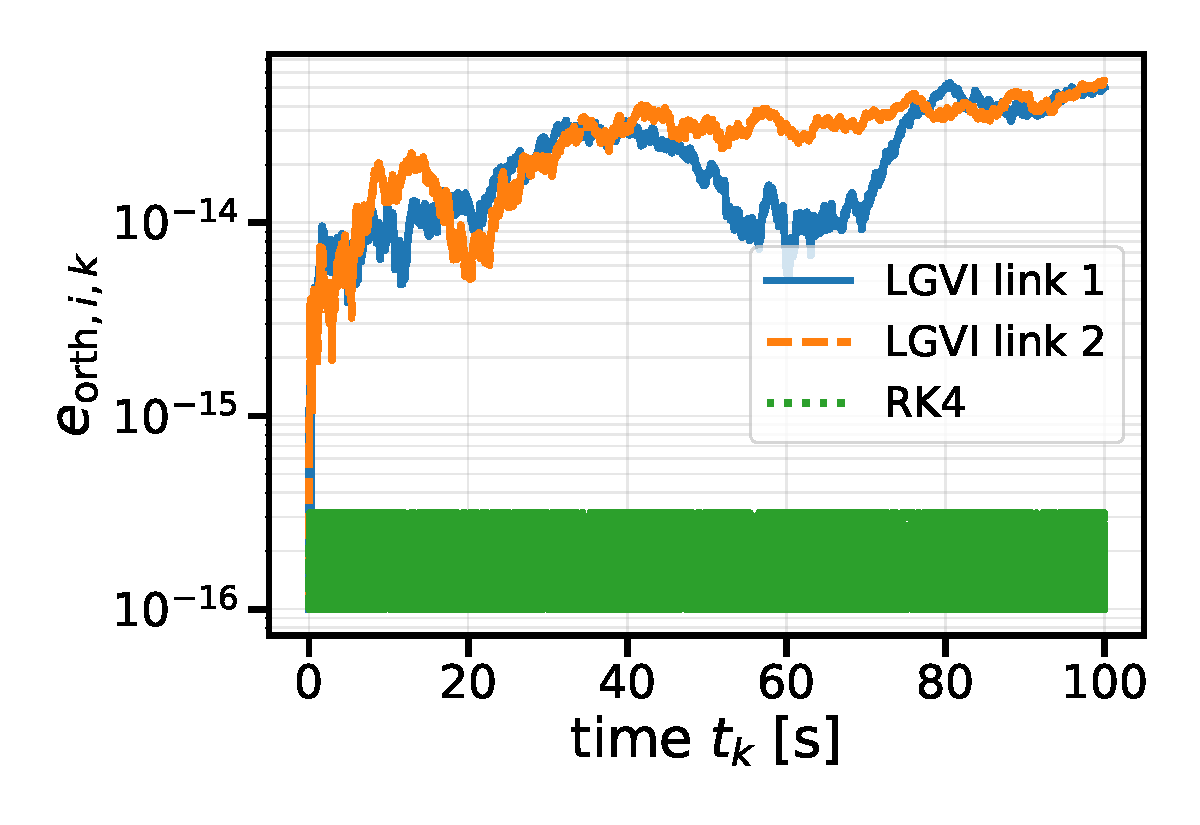
\includegraphics[width=\textwidth]{pics/Numerical_Simulation/Acrobot/forced_sine_orthogonality_error.pdf}
        \caption*{(d) Orthogonality error $e_{orth}$.}
    \end{minipage}

    \caption{Numerical simulation results for the controlled Acrobot.}
    \label{fig:simulation_results_acrobot_forced}
\end{figure}

The total energy \(E_k\) of the controlled Acrobot is shown in
Fig.~\ref{fig:simulation_results_acrobot_forced}(a). As for the controlled
3D pendulum, the LGVI and RK4 energies agree closely during approximately the
first $\SI{5}{\second}$ and subsequently deviate as the numerical trajectories
separate. In contrast to the unforced case, the applied torque performs work on
the system, and the mechanical energy is therefore neither conserved nor
expected to remain bounded around its initial value.

Fig.~\ref{fig:simulation_results_acrobot_forced}(b) shows the position error
norm $\|\Delta \bm{x}_k\|$ between the LGVI trajectory and the RK4 reference.
The error is initially zero and remains close to zero over the
first $\SI{5}{\second}$, confirming that both methods reproduce the same
short-time response to the sinusoidal elbow input. It then increases and
oscillates as the trajectories diverge, following the same
behaviour observed for the controlled 3D pendulum, because of the
numerical differences between the two methods.

The holonomic constraint residuals $\|\bm{\phi}_{0,k}\|_2$ and $\|\bm{\phi}_{12,k}\|_2$ are plotted in Fig.\ref{fig:simulation_results_acrobot_forced}(c). The base and elbow constraint residuals are negligible ($< 10^{-11}$) over the complete simulation. In the forced case, the maximal-coordinate LGVI therefore also prevents constraint drift and keeps the Acrobot links physically connected, which is essential for the later SDP optimization conducted in Section \ref{sec:acrobot_optimization_results}.

Finally, Fig.\ref{fig:simulation_results_acrobot_forced}(d) shows the orthogonality error $e_{orth,i,k}$ of both link rotations. As in the unforced simulation, the LGVI preserves the $SO(2)$ structure through the attitude update \eqref{eq:acrobot_full_del_shifted_kinematics_1} and \eqref{eq:acrobot_full_del_shifted_kinematics_2}. As in the unforced case, the RK4 reference remains close to zero, since its rotations are represented as rotation matrices. Therefore, the controlled Acrobot simulation confirms that both the forcing term and the constrained Lie-group update are numerically consistent.

Overall, Fig.~\ref{fig:simulation_results_acrobot_unforced} and
Fig.~\ref{fig:simulation_results_acrobot_forced} show that the Acrobot LGVI also behaves
consistently for a constrained multi-body system, introduced in Section \ref{sec:multi_body_systems}. The method preserves the
\(SO(2)\) structure, keeps the holonomic constraints small, and aligns closely with
the RK4 reference for the tested timestep.


\section{3D-Pendulum Optimization Results}
\label{sec:3d_pendulum_optimization_results}

This section evaluates the controlled 3D-pendulum polynomial optimization
problem (POP) \eqref{eq:controlled_3d_pendulum_pop} introduced in
Section~\ref{sec:discrete_motion_planning_3d_pendulum}. The POP is converted
into a sparse second-order Moment-SOS relaxation using SPOT and is solved with
MOSEK \cite{Kang_2025Global}. The implementation is documented in
\cite{Elshani2026CTO_GitHub}. All experiments were conducted 
on the Harvard FASRC Cannon cluster using Intel Xeon Sapphire Rapids CPUs and 
\(512\,\mathrm{GB}\) of RAM. Each optimization was executed on a 
single compute node using 8 CPU cores.

\paragraph{Optimization Configuration}
The physical parameters are identical to those used for the $3$D pendulum in
Section \ref{subsec:3d_pendulum_numercial_simulation}.
For all optimization runs, the
relaxation order, SDP time step, number of time steps, and prediction horizon
are
\begin{equation}
    \kappa=2,
    \qquad
    \Delta t_{\mathrm{SDP}}=0.1\,\mathrm{s},
    \qquad
    N=20,
    \qquad
    T=N\Delta t_{\mathrm{SDP}}=2.0\,\mathrm{s}.
    \label{eq:3d_pendulum_optimization_configuration}
\end{equation}
The initial attitude is $\bm{R}^{\mathrm{init}}=\bm{R}_x(5^\circ)$ and the initial
relative rotation is $\bm F^{\mathrm{init}}=\bm I$. Starting from the same
initial state, the desired rotation angle is varied as
\(\theta_{x,\mathrm{des}}\in
\{0^\circ,45^\circ,90^\circ,135^\circ,180^\circ\}\) around the x-axis, with
\(\bm{R}_{\mathrm{des}}=\bm{R}_x(\theta_{x,\mathrm{des}})\). The terminal 
desired relative rotation is chosen to be $\bm{F}_{\mathrm{des}}=\bm{I}$, which represents 
zero velocity at step $N$ of the 3D-pendulum.
The scalar control and relative-rotation limits of the POP are set as
\begin{align*}
    u_{\max}
    &=5,
    \\
    \cos(\Delta\theta_{\max})
    &=0.5.
\end{align*}
The objective parameters of \eqref{eq:controlled_3d_pendulum_pop_objective} 
remain constant for all target rotations and are
identical to the Acrobot optimization configuration in
Table \ref{tab:optimization_cost_parameters}.

The correlative sparsity pattern is completed with the minimum-degree (MD)
chordal-extension heuristic introduced in
Section~\ref{subsec:sparse_relaxations} \cite{Kang_2025Global}. For the present
problem, the largest clique generated by SPOT contains $24$ scalar variables.
Consequently, its order-two moment matrix has
\(\binom{24+2}{2}=325\) rows and columns. In comparison, the complete
$39$-variable temporal
chain-like clique $\bm{z}_{\mathrm{P}}(\mathcal I_k^{\mathrm{P}})$ would produce an $820\times820$ matrix, while the dense
relaxation for $N=20$ would require a
$91{,}378\times91{,}378$ matrix (see Section \ref{sec:discrete_motion_planning_3d_pendulum}).
Therefore, the MD chordal extension substantially
reduces the dense or chain-like moment-matrix in this experiment.

\paragraph{Evaluation metrics}
The angular rotation error at time step $k$ is
evaluated from the ordered SDP extraction in degrees as
\begin{equation}
    e_{R,k}^{P}
    =
    \frac{180}{\pi}\theta_{k}^{\mathrm{rad}},
    \qquad
    \theta_{k}^{\mathrm{rad}}
    =
    \cos^{-1}\!\left(
        \frac{\operatorname{tr}(\bm R_{\mathrm{des}}^\top\bm R_k)-1}{2}
    \right),
    \label{eq:3d_pendulum_evaluation_rotation_error}
\end{equation}
where $\theta_k^{\mathrm{rad}}$ is the relative rotation angle in radians and
$\bm{R}_{\mathrm{des}}^\top \bm{R}_k$ is the relative rotation to the target attitude
\cite{GallierQuaintance2020LinearAlgebra}. Thus, $e_{R,k}^{P}$ is reported in degrees.
Thereby, the terminal angular error at $N$
is denoted as $e_{R,N}^{P}$.
In addition, the maximum orthogonality violation over the optimization horizon is defined as
\begin{equation}
    e_{\mathrm{orth}}^{P,\max}
    =\max_{0\leq k\leq N}
    \left\lVert
        \bm R_k^{\top}\bm R_k-\bm I
    \right\rVert_F.
    \label{eq:3d_pendulum_evaluation_terminal_error}
\end{equation}

In order to evaluate the optimality of the lower-bound solution $\gamma_{\kappa}^*$,
a feasible upper bound $p(\widehat{\bm{z}})$ can be generated through a
nonlinear programming (NLP) solver \cite{Sangli2025}. Thereby, the corresponding 
objectives $J_{SDP}$ and $J_{NLP}$ can be calculated, whose suboptimality gap is given by 
\begin{equation}
    \epsilon
    =
    \frac{
        \left|J_{\mathrm{NLP}}-J_{\mathrm{SDP}}\right|
    }{
        \left|J_{\mathrm{NLP}}\right|+10^{-6}
    }.
    \label{eq:3d_pendulum_warm_start_gap}
\end{equation}
Here, the SDP trajectory extraction is used as a warm start for the NLP solver,
using the GitHub code of \cite{Sangli2025}. The resulting suboptimality gap is denoted by $\epsilon_{\mathrm{warm}}$.
The numerical rank condition $\delta_{\max}$ is evaluated according to
\eqref{eq:numerical_rank_metric} over the sub-moment matrices used for the
ordered extraction. The runtime given in Table \ref{tab:pendulum_3d_sdp_statistics} 
is the MOSEK optimizer time.

\begin{table}[!htbp]
    \centering
    \caption{Results of the controlled $3$D pendulum for desired $x$-axis rotations.}
    \label{tab:pendulum_3d_sdp_statistics}

    \setlength{\tabcolsep}{6pt}
    \renewcommand{\arraystretch}{1.15}

    \resizebox{\textwidth}{!}{%
    \begin{tabular}{@{}lccccc@{}}
        \toprule
        $\theta_{x,\mathrm{des}}$
        & $0^\circ$
        & $45^\circ$
        & $90^\circ$
        & $135^\circ$
        & $180^\circ$ \\
        \midrule

        Terminal angular error $e_{R,N}^{P}$
        & $0.0389^\circ$
        & $13.735^\circ$
        & $19.496^\circ$
        & $10.614^\circ$
        & $0.1418^\circ$ \\

        Manifold violation $e_{\mathrm{orth}}^{P,\max}$
        & $1.2\!\times\!10^{-9}$
        & $4.6\!\times\!10^{-8}$
        & $1.1\!\times\!10^{-11}$
        & $2.6\!\times\!10^{-9}$
        & $4.5\!\times\!10^{-8}$ \\

        Suboptimality gap $\epsilon_{warm}$
        & $1.8\!\times\!10^{-6}$
        & $8.8\!\times\!10^{-8}$
        & $5.6\!\times\!10^{-10}$
        & $2.4\!\times\!10^{-9}$
        & $2.8\!\times\!10^{-9}$ \\

        Rank condition $\delta_{\max}$
        & $3.0\!\times\!10^{-9}$
        & $7.3\!\times\!10^{-8}$
        & $1.1\!\times\!10^{-11}$
        & $3.2\!\times\!10^{-9}$
        & $2.3\!\times\!10^{-8}$ \\

        Runtime (s)
        & $3349.46$
        & $3706.36$
        & $4032.72$
        & $4128.29$
        & $3873.03$ \\
        \bottomrule
    \end{tabular}%
    }
\end{table}

\begin{figure}[t!]
    \centering
    \begin{minipage}{0.49\textwidth}
        \centering
        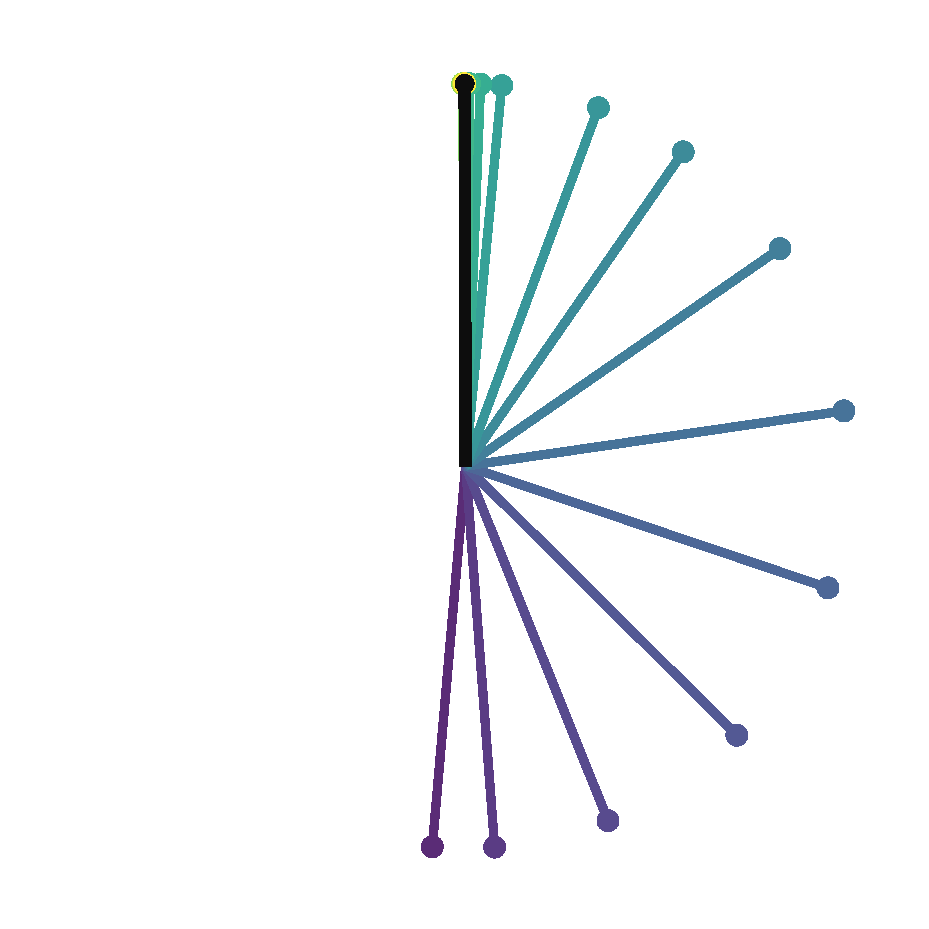
\includegraphics[width=0.70\linewidth]{pics/Optimization/3D_Pendulum/MD_180_deg_Pendulum_trajectory_matlab.pdf}
        \caption*{(a) 3D-Pendulum trajectory.}
    \end{minipage}
    \hfill
    \begin{minipage}{0.49\textwidth}
        \centering
        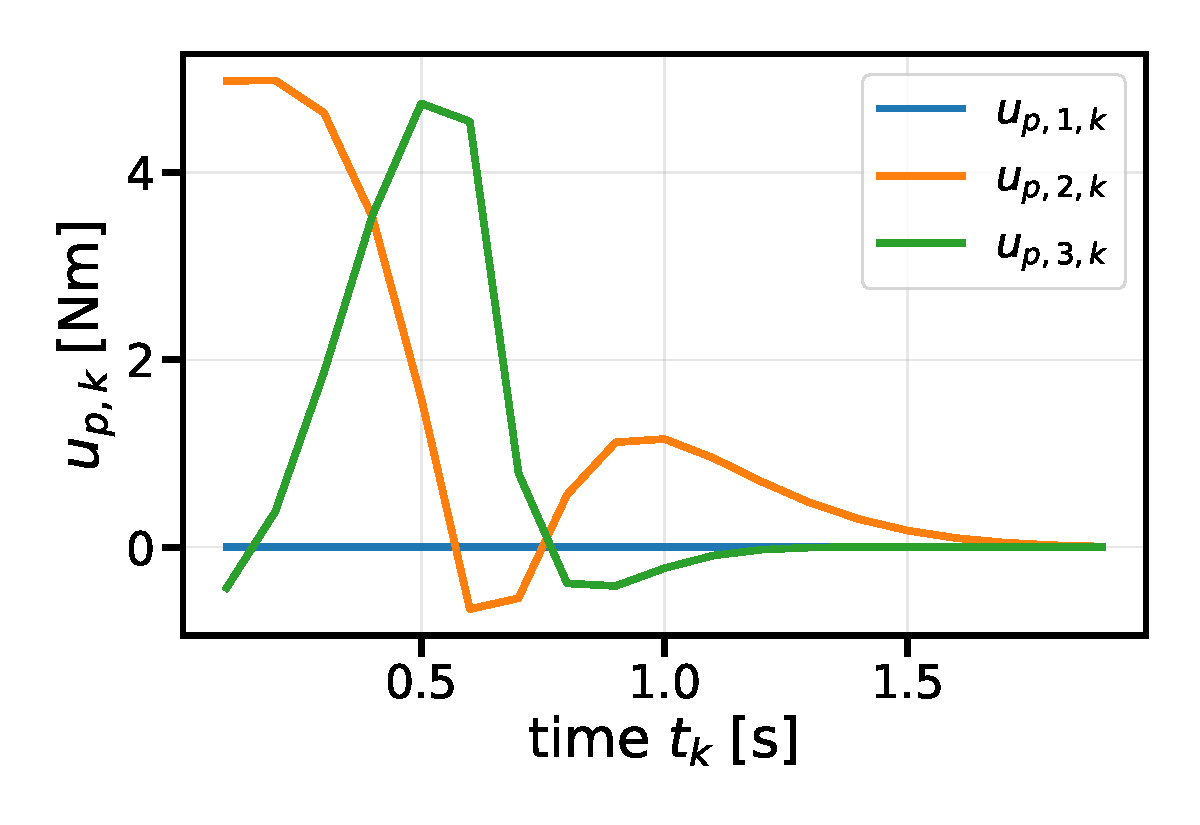
\includegraphics[width=\linewidth]{pics/Optimization/3D_Pendulum/MD_180_deg_Pendulum_control_input.pdf}
        \caption*{(b) Control inputs $\bm u_{p,k}$.}
    \end{minipage}

    \vspace{0.5em}

    \begin{minipage}{0.49\textwidth}
        \centering
        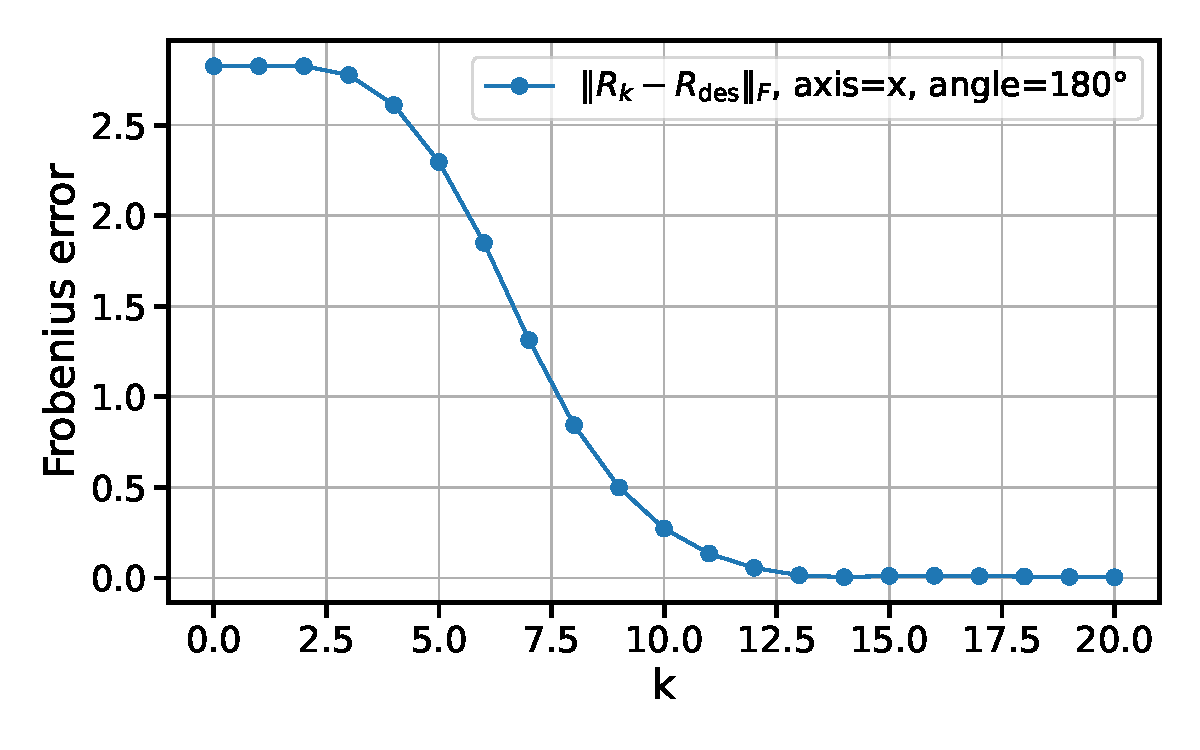
\includegraphics[width=\linewidth]{pics/Optimization/3D_Pendulum/MD_180_deg_Pendulum_frobenius.pdf}
        \caption*{(c) Angular rotation tracking error $e_{R,k}^{P}$.}
    \end{minipage}
    \hfill
    \begin{minipage}{0.49\textwidth}
        \centering
        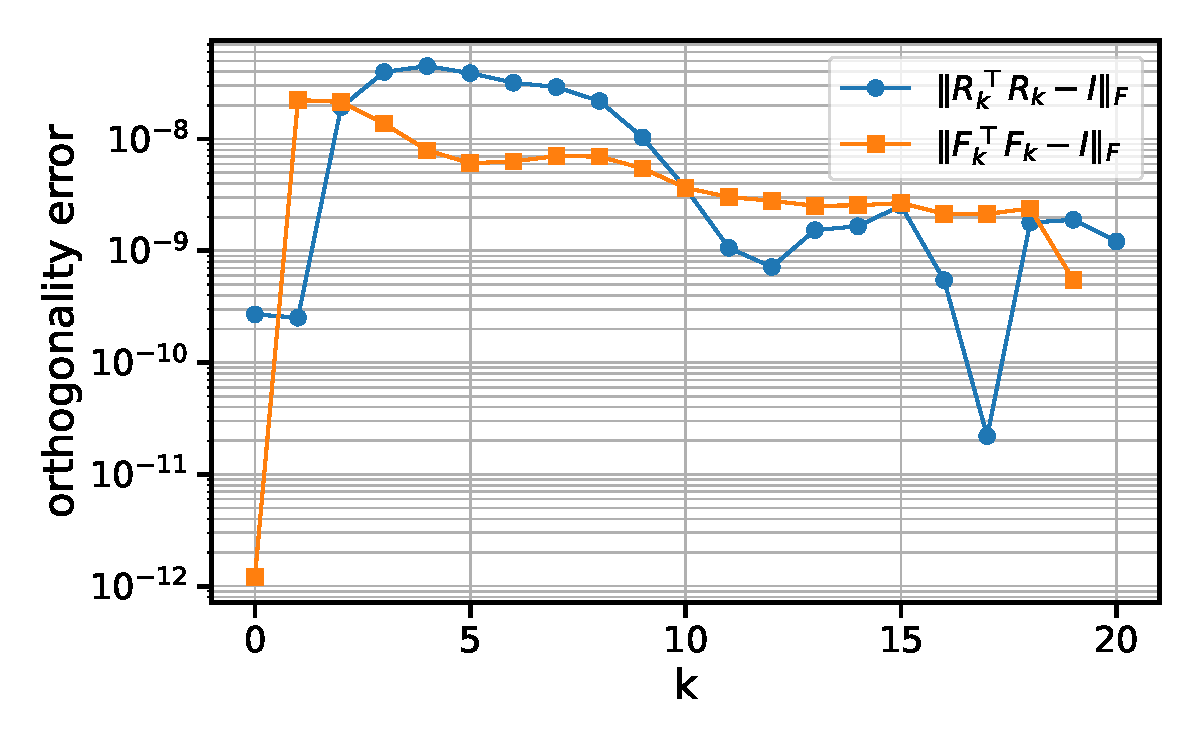
\includegraphics[width=\linewidth]{pics/Optimization/3D_Pendulum/MD_180_deg_Pendulum_orthogonality.pdf}
        \caption*{(d) Orthogonality errors $e_{\mathrm{orth},k}^{P}$ of
        $\bm R_k$, $\bm F_k$.}
    \end{minipage}

    \caption{SPOT optimization results for the controlled $3$D pendulum
    performing a $180^\circ$ rotation about the $x$-axis using the MD
    sparsity setting: (a) optimization trajectory,
    (b) control inputs
    $\bm u_{p,k}$, (c) angular rotation tracking error $e_{R,k}^{P}$, and
    (d) orthogonality errors $e_{\mathrm{orth},k}^{P}$}
    \label{fig:optimization_results_x180_md}
\end{figure}

\paragraph{Results}

Table~\ref{tab:pendulum_3d_sdp_statistics} shows that 
\(e_{\mathrm{orth}}^{P,\max}\leq4.6\times10^{-8}\) for all target rotations. Therefore, the 
extracted rotation matrices satisfy the orthogonality constraints. 
Moreover, \(\epsilon_{\mathrm{warm}}\leq1.8\times10^{-6}\) and 
\(\delta_{\max}\leq7.3\times10^{-8}\). The feasible NLP upper bounds and the SDP lower 
bounds therefore nearly coincide, while the maximal rank condition $\delta_{\max}$ of the 
evaluated sub-moment matrices is numerically 
close to rank one. Consequently, the suboptimality gap $\epsilon_{\mathrm{warm}}$ 
and rank metric validate the tightness
of the second-order MD relaxation for the considered 3D-pendulum test cases,
certifying the feasibility of the extracted solutions.

The terminal angular error does not increase monotonically with the target rotation
\(\theta_{x,\mathrm{des}}\). The smallest errors are obtained for the \(0^\circ\) and 
\(180^\circ\) targets, with \(e_{R,N}^{P}=0.0389^\circ\) and 
\(e_{R,N}^{P}=0.1418^\circ\). In contrast, the intermediate targets 
result in errors of \(13.735^\circ\), \(19.496^\circ\), and \(10.614^\circ\) for 
\(45^\circ\), \(90^\circ\), and \(135^\circ\). Consequently, the \(90^\circ\) target 
produces the largest terminal tracking error. The reason for this behaviour is that
the corresponding POP \eqref{eq:controlled_3d_pendulum_pop} does not require the 
optimal trajectory to reach the desired attitude exactly, as $\bm{R}_{\mathrm{des}}$ is not considered
as a hard terminal constraint but weighted in the objective. Furthermore, the \(0^\circ\) and 
\(180^\circ\) attitudes are equilibrium configurations of the considered pendulum for which 
the gravitational moment vanishes. In contrast, the intermediate attitudes require a 
control moment to stay at $\bm{R}_{\mathrm{des}}$, which contributes to their larger terminal errors. 

Fig.\ref{fig:optimization_results_x180_md} illustrates the ordered extraction 
for a desired rotation of \(\theta_{x,\mathrm{des}}=180^\circ\). The 
optimized trajectory follows a smooth path
from the initial to the inverted configuration.
As the rotation is around the x-axis, \(u_{p,1,k}\) 
remains zero. When reaching the final horizon time at $T=\SI{2}{\second}$, all three control
inputs approach zero. Correspondingly, the angular tracking error \(e_{R,k}^{P}\)
decreases from approximately \(175^\circ\) and reaches \(0.1418^\circ\) at the terminal time.
Finally, the orthogonality errors of both \(\bm R_k\) and \(\bm F_k\) remain less then
\(10^{-8}\), which validates the feasibility of the extracted solution. 
The four panels therefore show that the extracted trajectory performs the 
desired rotational motion while remaining on the Lie group.

\section{Acrobot Optimization Results}
\label{sec:acrobot_optimization_results}

This section evaluates the controlled Acrobot polynomial optimization problem
(POP) introduced in Section~\ref{sec:discrete_motion_planning_acrobot}. As for
the $3$D pendulum, SPOT constructs a sparse
second-order Moment-SOS relaxation, which is solved using MOSEK \cite{Kang_2025Global}. First, the
semidefinite optimization of
Section \ref{sec:trajectory_optimization_via_sdp_relaxation} is investigated.
For the larger desired rotations, its ordered extraction does not provide a
certified feasible trajectory over the complete horizon. This motivates the
closed-loop SDP--MPC formulation of
Section \ref{sec:acrobot_trajectory_optimization_SDP_MPC}, which applies only
the first extracted control before solving the problem again. The complete
implementation is documented in \cite{Elshani2026CTO_GitHub}. All experiments were conducted 
on the Harvard FASRC Cannon cluster using Intel Xeon Sapphire Rapids CPUs and 
\(512\,\mathrm{GB}\) of RAM. Each optimization was executed on a 
single compute node using 8 CPU cores.

\subsection{Semidefinite Optimization Results}
\label{subsec:acrobot_optimization_results}

\paragraph{Optimization configuration}
The physical parameters are identical to those of the Acrobot simulation in
Section~\ref{subsec:evaluation_acrobot}. For all optimization runs, the
relaxation order, SDP time step, and number of time steps are
\begin{equation}
    \kappa=2,
    \qquad
    \Delta t_{\mathrm{SDP}}=0.1\,\mathrm{s},
    \qquad
    N=60,
    \qquad
    N\Delta t_{\mathrm{SDP}}=6.0\,\mathrm{s}.
    \label{eq:acrobot_sdp_optimization_configuration}
\end{equation}
The complete discretization window from the history node $k=0$ to the terminal
node $k=N$ therefore spans $6.0\,\mathrm{s}$.

Both links start from the same initial attitude and relative rotation,
\begin{equation}
    \bm R_1^{\mathrm{init}}
    =\bm R_2^{\mathrm{init}}
    =\bm R(5^\circ),
    \qquad
    \bm F_1^{\mathrm{init}}
    =\bm F_2^{\mathrm{init}}
    =\bm I,
    \label{eq:acrobot_sdp_initial_configuration}
\end{equation}
where $\bm R(\theta)\in SO(2)$ denotes the planar rotation matrix defined in
\eqref{eq:so2_rotation_matrix}. Starting from this state, the same desired
absolute rotation is assigned to both links
\begin{equation}
    \theta_1^{\mathrm{des}}
    =\theta_2^{\mathrm{des}}
    =\theta_{\mathrm A}^{\mathrm{des}}
    \in
    \{0^\circ,45^\circ,90^\circ,135^\circ,180^\circ\},
    \label{eq:acrobot_sdp_target_configurations}
\end{equation}
with desired relative rotation $\bm F_1^{\mathrm{des}}
    =\bm F_2^{\mathrm{des}}
    =\bm I_2$ after $N=60$.
In particular, $\theta_{\mathrm A}^{\mathrm{des}}=180^\circ$ represents the inverted
equilibrium with both links at rest, which is considered as a final stabilization target for the Acrobot.
The physical control and multiplier scales
of \eqref{eq:acrobot_variable_scaling}, together with the link-specific rotation
increment bounds in \eqref{eq:controlled_acrobot_pop_step_bound}, are chosen as
\begin{equation}
    u_{\max}=15\,\mathrm{N\,m},
    \qquad
    \lambda_{\max}=40\,\mathrm{N},
    \qquad
    \Delta\theta_{1,\max}=70^\circ,
    \qquad
    \Delta\theta_{2,\max}=60^\circ.
    \label{eq:acrobot_sdp_optimization_bounds}
\end{equation}
Thus, the polynomial step constraints are
$a_{1,k}\geq\cos(70^\circ)\approx0.3420$ and
$a_{2,k}\geq\cos(60^\circ)=0.5$ for $k=1,\ldots,N-1$. The objective parameters of the 
cost function \eqref{eq:controlled_acrobot_pop_objective} are summarized in
Table~\ref{tab:optimization_cost_parameters}.

\begin{table}[!htbp]
    \centering
    \caption{Objective parameters used for the $3$D-pendulum and Acrobot
    optimization experiments.}
    \label{tab:optimization_cost_parameters}
    \setlength{\tabcolsep}{12pt}
    \renewcommand{\arraystretch}{1.15}
    \begin{tabular}{@{}ccccc@{}}
        \toprule
        $w_R$ & $w_F$ & $\alpha_R$ & $\alpha_F$ & $w_u$ \\
        \midrule
        $20$ & $8$ & $15$ & $2$ & $0.09$ \\
        \bottomrule
    \end{tabular}
\end{table}

Two user-defined clique constructions are compared. The first follows the
complete chain-like sparsity of
\eqref{eq:acrobot_full_self_initial_clique}--\eqref{eq:acrobot_full_self_interior_cliques}.
At $\kappa=2$, its first clique
$\bm{z}_{\mathrm{A}}(\mathcal I_1^{\mathrm{A}})$ produces a $351\times351$ moment
matrix, while every subsequent complete clique
$\bm{z}_{\mathrm{A}}(\mathcal I_k^{\mathrm{A}})$ produces a
$253\times253$ matrix, as given in
\eqref{eq:acrobot_full_self_moment_sizes}. The second construction uses the
special multi-body sparsity in \eqref{eq:acrobot_hybrid_self_cliques}. It keeps
the complete cliques $\bm{z}_{\mathrm{A}}(\mathcal I_1^{\mathrm{A}})$ and
$\bm{z}_{\mathrm{A}}(\mathcal I_2^{\mathrm{A}})$,
but separates the later coupled dynamics
$\bm{z}_{\mathrm{A}}(\mathcal I_{\mathrm{dyn},k}^{\mathrm{A}})$ and kinematics
$\bm{z}_{\mathrm{A}}(\mathcal I_{\mathrm{kin},k}^{\mathrm{A}})$ into moment matrices
of size $171\times171$ and $91\times91$
\eqref{eq:acrobot_hybrid_self_moment_sizes}. Consequently,
the larger cliques around the first control decision are preserved, whereas the
semidefinite blocks over the remaining horizon are reduced.

\paragraph{Evaluation metrics}
Similar to the $3$D-pendulum evaluation \eqref{eq:3d_pendulum_evaluation_rotation_error}, the terminal attitude error is
reported in degrees. The combined
angular error of both links is defined as
\begin{equation}
\begin{aligned}
e_{R,k}^{\mathrm A}
&:=
\frac{180^\circ}{\pi}
\left(
    \sum_{i=1}^{2}
    \left(\theta_{i,k}^{\mathrm{rad}}\right)^2
\right)^{1/2},
\\
\theta_{i,k}^{\mathrm{rad}}
&:=
\cos^{-1}\!\left(
\frac{
\operatorname{tr}\!\left(
(\bm R_i^{\mathrm{des}})^\top
\bm R_{i,k}
\right)
}{2}
\right),
\end{aligned}
\label{eq:acrobot_terminal_rotation_error}
\end{equation}
for $i\in\{1,2\}$.
The angular error $e_{R,k}^{\mathrm A}$ is the Euclidean combination of the two
link-wise angular errors. Thereby, $e_{R,N}^{\mathrm A}$ is interpreted as a
terminal matrix error at $k=N$.
The maximum orthogonality violation is evaluated over the configuration of both links by
\begin{equation}
\begin{aligned}
    e_{\mathrm{orth}}^{\mathrm A,\max}
    =\max_{\substack{i\in\{1,2\}\\0\leq k\leq N-1}}
    \left\|
        \bm R_{i,k}^{\top}\bm R_{i,k}-\bm I_2
    \right\|_F.
\end{aligned}
\label{eq:acrobot_max_orthogonality_error}
\end{equation}
The relative-rotation errors of $\bm{F}_{i,k}$ are smaller than $\bm{R}_{i,k}$ for all $k$.
Therefore, the orthogonality of $\bm{F}_{i,k}$ is not evaluated.

The maximum numerical rank condition $\delta_{\max}$ is evaluated according to
\eqref{eq:numerical_rank_metric}~\cite{Sangli2025}. Additionally, the rank condition
of the first moment matrix, which belongs to the
clique vector \(\bm{z}_{\mathrm{A}}(\mathcal I_1^{\mathrm{A}})\), is denoted by
\begin{equation}
    \delta_1
    :=
    \frac{\nu_{2,1}}{\nu_{1,1}},
    \qquad
    \nu_{1,1}\geq\nu_{2,1}\geq0.
    \label{eq:acrobot_first_clique_rank_metric}
\end{equation}
Here, $\nu_{1,1}$ and $\nu_{2,1}$ are the two largest eigenvalues of
the moment matrix associated with
\(\bm{z}_{\mathrm{A}}(\mathcal I_1^{\mathrm{A}})\). The quantity
\(\delta_1\) is reported in addition to \(\delta_{\max}\) because
\(\bm{z}_{\mathrm{A}}(\mathcal I_1^{\mathrm{A}})\) contains the first normalized control
$\bar u_1$ used later by the subsequent MPC controller.

In contrast to the $3$D pendulum, the extracted SDP trajectories for the
Acrobot POP with $N=60$ were not certifiable for all targets. Therefore,
cold-start NLP upper bounds were generated instead of using the SDP extraction
as a warm start. The reported suboptimality gap
$\epsilon_{\mathrm{cold}}$ is computed according to
\eqref{eq:3d_pendulum_warm_start_gap} with the cold-start NLP objective. The
runtimes in Tables~\ref{tab:acrobot_sdp_statistics_full} and
\ref{tab:acrobot_sdp_statistics_hybrid} are the solver operation times reported
by the implementation.

\begin{table}[H]
    \centering
    \caption{Results of the Acrobot trajectory optimization using the
    complete chain-like cliques
    \(\bm{z}_{\mathrm{A}}(\mathcal I_k^{\mathrm{A}})\). All trajectory metrics are
    evaluated from the
    ordered extraction.}
    \label{tab:acrobot_sdp_statistics_full}
    \setlength{\tabcolsep}{6pt}
    \renewcommand{\arraystretch}{1.15}
    \resizebox{\textwidth}{!}{%
    \begin{tabular}{@{}lccccc@{}}
        \toprule
        $\theta_1^{\mathrm{des}}=\theta_2^{\mathrm{des}}$
        & $0^\circ$ & $45^\circ$ & $90^\circ$ & $135^\circ$ & $180^\circ$ \\
        \midrule
        Terminal angular error $e_{R,N}^{\mathrm A}$
        & $3.2815^\circ$
        & $54.975^\circ$
        & $64.629^\circ$
        & $36.377^\circ$
        & $3.1\!\times\!10^{-4}\,{}^\circ$ \\
        Manifold violation $e_{\mathrm{orth}}^{\mathrm A,\max}$
        & $2.2\!\times\!10^{-8}$ & $1.9\!\times\!10^{-8}$
        & $1.0368$ & $1.3688$ & $1.4053$ \\
        Suboptimality gap $\epsilon_{\mathrm{cold}}$
        & $2.0\!\times\!10^{-6}$ & $4.8\!\times\!10^{-10}$
        & $0.0717$ & $0.4126$ & $0.5233$ \\
        Rank condition $\delta_{\max}$
        & $1.4\!\times\!10^{-8}$ & $1.1\!\times\!10^{-8}$
        & $0.3542$ & $0.4696$ & $0.5596$ \\
        Rank condition $\delta_1$
        & $3.1\!\times\!10^{-9}$ & $2.8\!\times\!10^{-10}$
        & $0.003747$ & $0.1020$ & $0.2066$ \\
        Runtime $[\mathrm{s}]$
        & $2675.54$ & $3581.13$ & $6806.96$ & $5913.05$ & $5421.42$ \\
        \bottomrule
    \end{tabular}%
    }
\end{table}

\begin{table}[H]
    \centering
    \caption{Results of the Acrobot trajectory optimization using the
    special multi-body clique construction
    \(\bm{z}_{\mathrm{A}}(\mathcal I_1^{\mathrm{A}})\),
    \(\bm{z}_{\mathrm{A}}(\mathcal I_2^{\mathrm{A}})\),
    \(\bm{z}_{\mathrm{A}}(\mathcal I_{\mathrm{dyn},k}^{\mathrm{A}})\), and
    \(\bm{z}_{\mathrm{A}}(\mathcal I_{\mathrm{kin},k}^{\mathrm{A}})\).
    All metrics are defined as in
    Table~\ref{tab:acrobot_sdp_statistics_full}.}
    \label{tab:acrobot_sdp_statistics_hybrid}
    \setlength{\tabcolsep}{6pt}
    \renewcommand{\arraystretch}{1.15}
    \resizebox{\textwidth}{!}{%
    \begin{tabular}{@{}lccccc@{}}
        \toprule
        $\theta_1^{\mathrm{des}}=\theta_2^{\mathrm{des}}$
        & $0^\circ$ & $45^\circ$ & $90^\circ$ & $135^\circ$ & $180^\circ$ \\
        \midrule
        Terminal angular error $e_{R,N}^{\mathrm A}$
        & $3.2815^\circ$
        & $54.975^\circ$
        & $65.192^\circ$
        & $36.378^\circ$
        & $3.6\!\times\!10^{-4}\,{}^\circ$ \\
        Manifold violation $e_{\mathrm{orth}}^{\mathrm A,\max}$
        & $3.0\!\times\!10^{-12}$ & $3.4\!\times\!10^{-6}$
        & $1.0225$ & $1.4103$ & $1.4561$ \\
        Suboptimality gap $\epsilon_{\mathrm{cold}}$
        & $1.1\!\times\!10^{-10}$ & $9.2\!\times\!10^{-9}$
        & $0.0778$ & $0.4500$ & $0.5668$ \\
        Rank condition $\delta_{\max}$
        & $2.1\!\times\!10^{-12}$ & $2.4\!\times\!10^{-6}$
        & $0.4216$ & $0.4046$ & $0.6603$ \\
        Rank condition $\delta_1$
        & $2.6\!\times\!10^{-13}$ & $2.4\!\times\!10^{-8}$
        & $0.0010$ & $0.0973$ & $0.2172$ \\
        Runtime $[\mathrm{s}]$
        & $904.83$ & $1058.08$ & $1356.14$ & $1524.25$ & $1869.36$ \\
        \bottomrule
    \end{tabular}%
    }
\end{table}

\paragraph{Results}

Tables~\ref{tab:acrobot_sdp_statistics_full} and
\ref{tab:acrobot_sdp_statistics_hybrid} show the same qualitative behavior for
both clique constructions. For the $0^\circ$ and $45^\circ$ targets,
$\delta_{\max}$ and $e_{\mathrm{orth}}^{\mathrm A,\max}$ remain of
order $10^{-6}$. Moreover, all corresponding cold-start suboptimality gaps
satisfy $\epsilon_{\mathrm{cold}}\leq2.0\times10^{-6}$. Thus, the feasible NLP
upper bounds and the SDP lower bounds nearly coincide, while the evaluated
moment matrices are numerically close to rank one. The extracted matrices
satisfy the $SO(2)$ constraints up to a small tolerance. Together, these
metrics provide strong numerical evidence that the second-order relaxations
are tight and provide a certificate for these two cases.

The complete chain-like and special multi-body constructions give combined
terminal angular errors of $54.975^\circ$ for the $45^\circ$ target, 
This comparatively large
terminal error does not contradict the observed tightness because the desired
attitudes are included as objective terms and are not imposed as terminal
constraints. Similar to the $3$D pendulum results in
Section~\ref{sec:3d_pendulum_optimization_results}, this target is 
not an equilibrium configuration of the Acrobot.

For desired rotations of $90^\circ$, $135^\circ$, and $180^\circ$, the
definition of chain-like cliques gives terminal angular errors of $64.629^\circ$,
$36.377^\circ$, and
$3.1449\!\times\!10^{-4}\,{}^\circ$. The corresponding values
for the special multi-body construction are $65.192^\circ$,
$36.378^\circ$, and
$3.6388\!\times\!10^{-4}\,{}^\circ$. However, these terminal orientation
errors alone do not establish feasibility.

For these three targets, the values of $\delta_{\max}$ lie between $0.3542$
and $0.6603$, while $e_{\mathrm{orth}}^{\mathrm A,\max}$ lies between
$1.0225$ and $1.4561$. Consequently, the raw ordered extraction does
not represent a feasible $SO(2)$ trajectory over the complete horizon, and the
rank-one condition does not provide tightness. In particular, the 
$180^\circ$ results illustrate why both metrics must be considered together.
Although the projected terminal angular error is below
$4\!\times\!10^{-4}\,{}^\circ$, it has the highest
suboptimality gap and the largest manifold violation among all target rotations.

The cold-start NLP solutions provide
valid upper bounds for these cases. Nevertheless, the suboptimality gaps 
$\epsilon_{\mathrm{cold}}$ are
$0.0717$ and $0.0778$ for the $90^\circ$ target, $0.4126$ and $0.4500$ for
the $135^\circ$ target, and $0.5233$ and $0.5668$ for the $180^\circ$ target
for the complete chain-like and special multi-body constructions.
These large suboptimality gaps alone do not prove that the relaxation
is non-tight as it may also be a result of a suboptimal NLP upper bound \cite{Sangli2025}.
However, the higher-rank moment matrices and infeasible ordered
extractions show that global optimality is not certified for
these three cases.

Nevertheless, $\delta_1$ is smaller than $\delta_{\max}$ in every test case.
For example, the $90^\circ$ target gives $\delta_1=0.0037$
compared with $\delta_{\max}=0.3542$ for the chain-like cliques. Moreover, the 
special multi-body clique construction gives $\delta_1=0.0010$ compared with 
$\delta_{\max}=0.4216$. Consequently, the first
moment block is considerably closer to rank one than $\delta_{\max}$,
even if the moment blocks with values between $0.10$ and
$0.22$ for the $135^\circ$ and $180^\circ$ targets are generally not rank one.


The special multi-body construction produces terminal, manifold,
suboptimality-gap, and rank metrics that are comparable to the complete
chain-like construction, while its runtime is approximately $3$ to $5$
times smaller. Therefore, it is used for the following closed-loop evaluation
in Section \ref{subsec:acrobot_sdp_mpc_results}.



\subsection{Model Predictive SDP Control Results}
\label{subsec:acrobot_sdp_mpc_results}

The open-loop results of
Section~\ref{subsec:acrobot_optimization_results} show that the first-clique
rank metric $\delta_1$ is substantially smaller than the worst rank metric
$\delta_{\max}$ for all test cases (see Table \ref{tab:acrobot_sdp_statistics_hybrid}).
This observation motivates the SDP-MPC formulation of
Section~\ref{sec:acrobot_trajectory_optimization_SDP_MPC}. At every MPC
iteration, the second-order sparse Moment-SOS relaxation of the Acrobot
POP~\eqref{eq:controlled_acrobot_pop} is solved, only the first extracted control
$u_j$ in \eqref{eq:acrobot_mpc_applied_control} is applied, and the numerical
LGVI dynamics \eqref{eq:acrobot_full_del_shifted} 
are propagated (see Section \ref{subsec:evaluation_acrobot}).
The remaining predicted trajectory is ignored and the boundary data are
updated from the simulated state before the next SDP is solved. The purpose of
the following experiments is to determine whether this repeated first-step
extraction can stabilize the Acrobot at the inverted equilibrium of 
\begin{align}\label{eq:acrobot_stabilization_target}
    \theta_{\mathrm A}^{\mathrm{des}} = 180^\circ,
    \qquad
    \bm{F}^{des}_1=\bm{F}^{des}_2=\bm{I},
\end{align}
even when the
complete predicted SDP trajectory is not certifiable.

\paragraph{MPC configuration for $u_{\max}=5\,\mathrm{N\,m}$}
The physical Acrobot parameters are identical to those used for the numerical
simulation in Section~\ref{subsec:evaluation_acrobot}, and the objective
parameters are those in Table~\ref{tab:optimization_cost_parameters}. The
second-order relaxation uses only the special multi-body clique
construction in \eqref{eq:acrobot_hybrid_self_cliques}. As shown in the
preceding open-loop comparison, this construction preserves the complete first
two cliques (\(\bm{z}_{\mathrm{A}}(\mathcal I_1^{\mathrm{A}})\),
\(\bm{z}_{\mathrm{A}}(\mathcal I_2^{\mathrm{A}})\)),
including the first applied control, while reducing the sizes of
the moment blocks at $k=3,\dots,N_{\mathrm{SDP}}-1$ using
\(\bm{z}_{\mathrm{A}}(\mathcal I_{\mathrm{dyn},k}^{\mathrm{A}})\) and
\(\bm{z}_{\mathrm{A}}(\mathcal I_{\mathrm{kin},k}^{\mathrm{A}})\).

Both links start at rest from an absolute rotation of $5^\circ$
\begin{equation}
\begin{aligned}
    \bm R_1^{\mathrm{init}}
    &=\bm R_2^{\mathrm{init}}=\bm R(5^\circ),
    &\qquad
    \bm F_1^{\mathrm{init}}
    &=\bm F_2^{\mathrm{init}}=\bm I_2.
\end{aligned}
\label{eq:acrobot_mpc_u5_boundary_configurations}
\end{equation}
The relaxation order, time scales, and horizon are
\begin{equation}
    \kappa=2,
    \qquad
    \Delta t_{\mathrm{SDP}}
    =\Delta t_{\mathrm{sim}}
    =\Delta t_{\mathrm{ctrl}}
    =0.1\,\mathrm{s},
    \qquad
    N_{\mathrm{SDP}}=30.
\label{eq:acrobot_mpc_u5_time_configuration}
\end{equation}
Consequently, the complete discretization during each SDP iteration spans
$3.0\,\mathrm{s}$.
The bounds are
\begin{equation}
    u_{\max}=5\,\mathrm{N\,m},
    \qquad
    \lambda_{\max}=40\,\mathrm{N},
    \qquad
    \Delta\theta_{1,\max}=70^\circ,
    \qquad
    \Delta\theta_{2,\max}=60^\circ.
\label{eq:acrobot_mpc_u5_bounds}
\end{equation}
Therefore, only the torque bound $u_{\max}$ differs from the bounds used for the open-loop
experiments in \eqref{eq:acrobot_sdp_optimization_bounds}.

Stabilization is achieved if the simulated state
\eqref{eq:acrobot_mpc_stabilization_condition} is reached. The attitude and
relative-step rotation tolerances are $\varepsilon_R=2^\circ$ and
$\varepsilon_F=2^\circ$. Both conditions must hold for
three consecutive MPC updates $n_{\mathrm{stable}}=3$. 
No NLP correction or fallback controller is used. The closed-loop experiment
is limited to a maximum of $N_{\mathrm{MPC}}=600$ MPC iterations, which corresponds
to a maximum simulated duration of $60\,\mathrm{s}$.

\begin{figure}[t]
    \centering
    \begin{minipage}{0.49\textwidth}
        \centering
        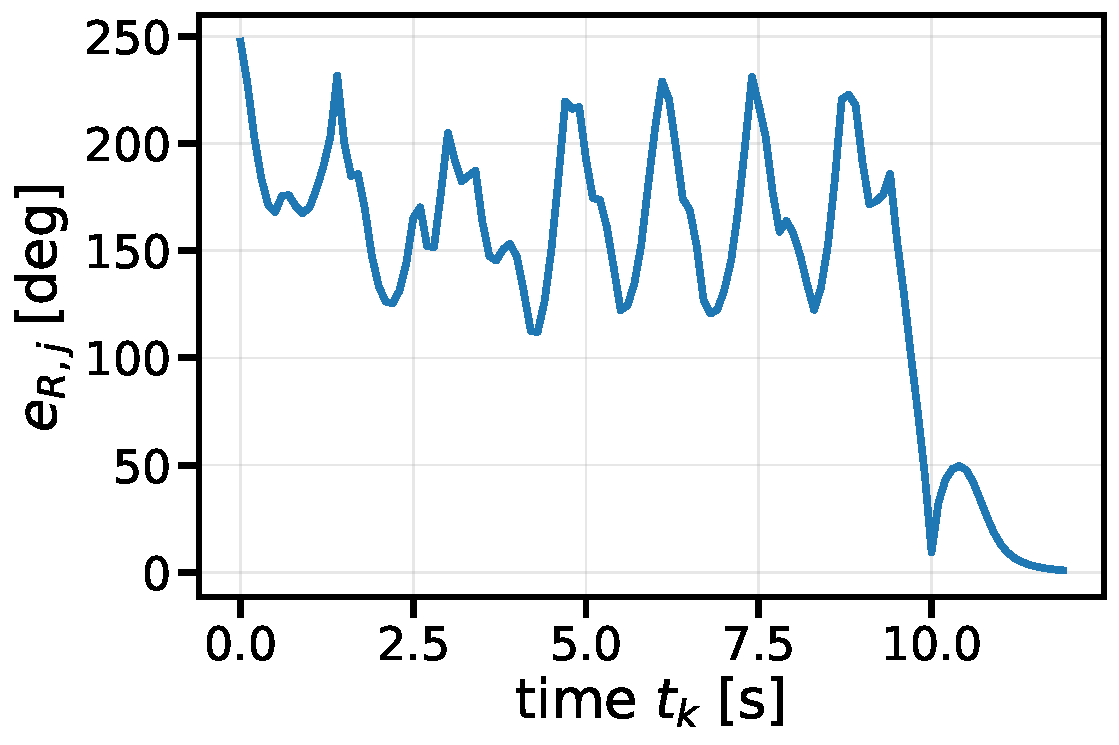
\includegraphics[width=\textwidth]{pics/Optimization/Acrobot/u5_target_rotation_error_norm.pdf}
        \caption*{(a) Target-attitude error $e_{R,j}$.}
    \end{minipage}
    \hfill
    \begin{minipage}{0.49\textwidth}
        \centering
        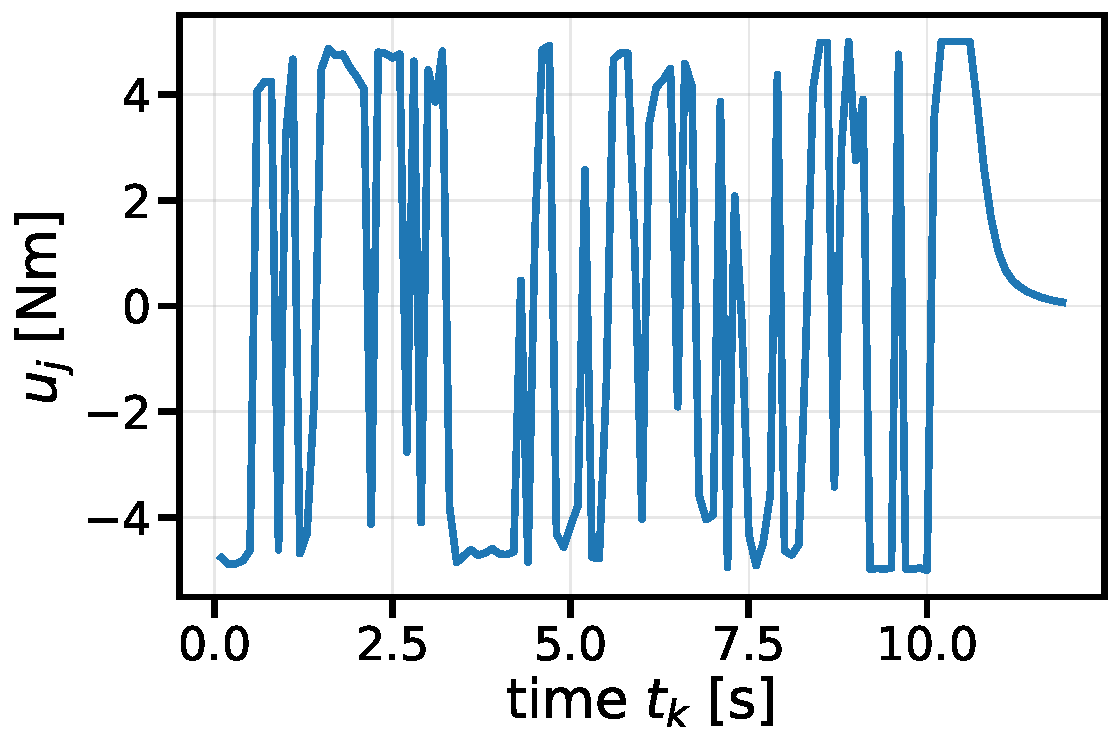
\includegraphics[width=\textwidth]{pics/Optimization/Acrobot/u5_control_inputs.pdf}
        \caption*{(b) Applied MPC control input $u_j$.}
    \end{minipage}

    \vspace{0.5em}

    \begin{minipage}{0.49\textwidth}
        \centering
        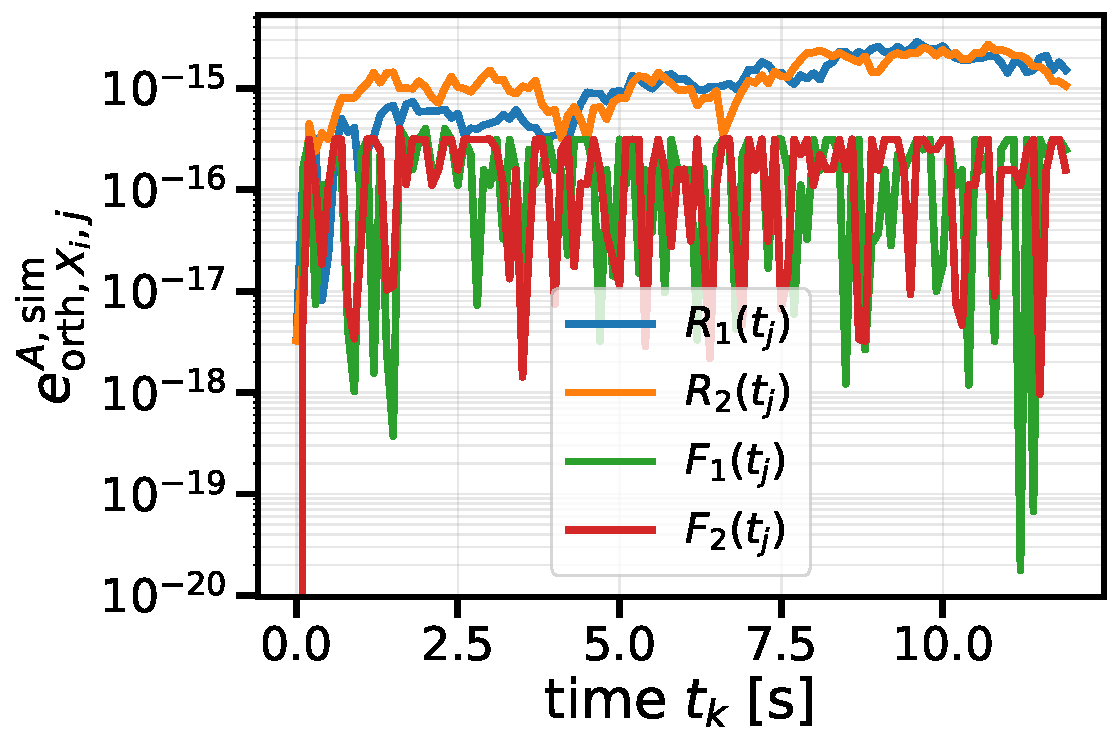
\includegraphics[width=\textwidth]{pics/Optimization/Acrobot/u5_SO2_errors_R_F.pdf}
        \caption*{(c) $SO(2)$ errors of $\bm{X}_{i,j}$.}
    \end{minipage}
    \hfill
    \begin{minipage}{0.49\textwidth}
        \centering
        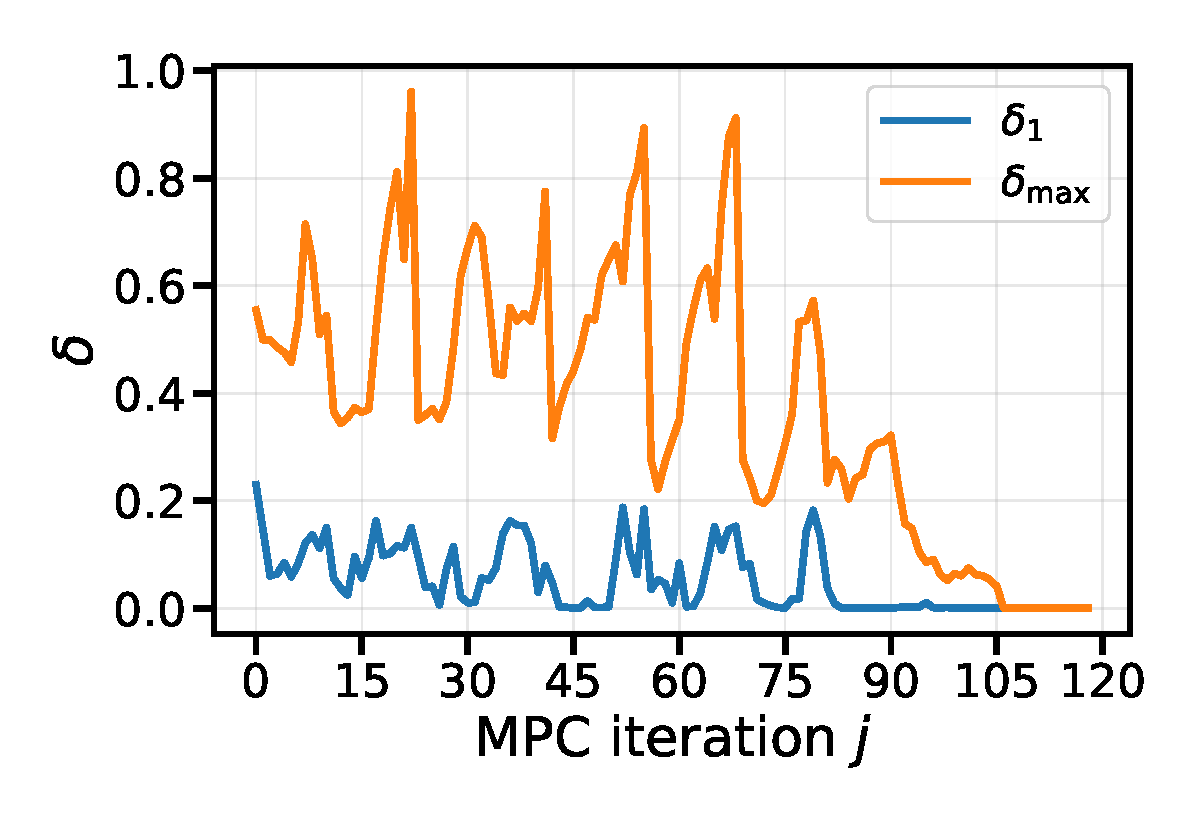
\includegraphics[width=\textwidth]{pics/Optimization/Acrobot/rank_condition_u5.pdf}
        \caption*{(d) Rank metrics $\delta_1$ and $\delta_{\max}$.}
    \end{minipage}

    \caption{Closed-loop SDP--MPC results for the Acrobot with
    $u_{\max}=5\,\mathrm{N\,m}$.}
    \label{fig:acrobot_mpc_u5_closed_loop}
\end{figure}

\paragraph{Results for $u_{\max}=5\,\mathrm{N\,m}$}
Figure \ref{fig:acrobot_mpc_u5_closed_loop} shows one successful closed-loop
swing-up and achieved stabilization. The combined starting attitude error
$e_{R,1}^A$ at $j=1$ is approximately
$247.5^\circ$. The error remains large and oscillates during
the swing up sequence. It begins to decrease rapidly after
approximately $9.5\,\mathrm{s}$ and remains close to zero after approximately
$11.9\,\mathrm{s}$. Therefore, the controller generates a swing-up motion
before stabilizing the Acrobot near the inverted equilibrium (see Fig \ref{fig:acrobot_mpc_u5_closed_loop}(a)).

In Fig.~\ref{fig:acrobot_mpc_u5_closed_loop}(b), the control input repeatedly reaches both limits of
$\pm5\,\mathrm{N\,m}$ during most of the swing-up and decreases toward zero
near the target. The torque constraint is therefore active and restricts
the available corrective action. 

Fig.~\ref{fig:acrobot_mpc_u5_closed_loop}(c) 
illustrates that
the orthogonality errors of the simulated $\bm R_i$ and $\bm F_i$ remain
below $10^{-15}$ without a growing drift. 
Therefore, the generated numerical LGVI trajectory remains
on $SO(2)$. However, the
raw predicted trajectories extracted from the individual SDP problems are
not feasible.

The rank metrics in Fig.~\ref{fig:acrobot_mpc_u5_closed_loop}(d) gives the
corresponding relaxation diagnostic. During a large part of the experiment,
$\delta_1$ assumes values up to approximately $0.2$, while
$\delta_{\max}$ reaches values close to $1$. The first moment block is
therefore generally closer to rank one than the worst block over the horizon.
Still it is not rank one throughout the full
swing-up process. The two metrics are simultaneously close to zero only near
stabilization. 

Finally, the implemented closed-loop SDP optimization
establishes a successful numerical closed-loop
stabilization for the considered initial state. Nevertheless,
the SDP-predicted trajectories do not provide a global optimality 
certificate for the applied control sequence.

The $5\,\mathrm{N\,m}$ bound was not sufficient across all additional tested
initial configurations. For configurations that require
stronger counteracting torques, the controller has limited capability
to provide sufficient corrective action. The following evaluation 
therefore increases the bound to 
$u_{\max}=15\,\mathrm{N\,m}$ and investigates a grid of initial link
orientations.

\paragraph{Empirical basin of attraction and time-discretization mismatch}
For this evaluation, the physical parameters, the relaxation order $\kappa=2$,
the target in \eqref{eq:acrobot_stabilization_target}, the objective
parameters, the multiplier and step-angle bounds, and the special multi-body cliques remain unchanged. Of the optimization bounds, only the control
bound is increased to $u_{\max}=15\,\mathrm{N\,m}$. Three combinations 
of prediction, simulation,
and control time scales are considered, as summarized in
Table~\ref{tab:acrobot_mpc_time_scale_cases}.

\begin{table}[!htbp]
    \centering
    \caption{Time-scale configurations used for the sampled SDP--MPC
    stabilization regions with $u_{\max}=15\,\mathrm{N\,m}$.}
    \label{tab:acrobot_mpc_time_scale_cases}
    \setlength{\tabcolsep}{7pt}
    \renewcommand{\arraystretch}{1.15}
    \begin{tabular}{@{}cccccc@{}}
        \toprule
        Case & $\Delta t_{\mathrm{SDP}}$ & $\Delta t_{\mathrm{sim}}$
        & $\Delta t_{\mathrm{ctrl}}$ & $N_{\mathrm{SDP}}$ & Time scales \\
        \midrule
        I   & $0.1\,\mathrm{s}$  & $0.1\,\mathrm{s}$
            & $0.1\,\mathrm{s}$   & $20$ & matched \\
        II  & $0.05\,\mathrm{s}$ & $0.05\,\mathrm{s}$
            & $0.05\,\mathrm{s}$  & $40$ & matched \\
        III & $0.1\,\mathrm{s}$  & $0.0025\,\mathrm{s}$
            & $0.025\,\mathrm{s}$ & $20$ & mismatched \\
        \bottomrule
    \end{tabular}
\end{table}

In both Cases~I and II, the prediction, plant, and control intervals are
matched. In both cases, the total prediction horizon is
$N_{\mathrm{SDP}}\Delta t_{\mathrm{SDP}}=2.0\,\mathrm{s}$. Case II
therefore evaluates whether a consistent refinement of all time scales changes
the sampled stabilization result while retaining approximately the same
prediction horizon time. In Case III, the prediction model uses the same
$0.1\,\mathrm{s}$ step as Case I, but the simulation model uses
fine LGVI steps of $\Delta t_{\mathrm{sim}}=0.0025\,\mathrm{s}$ 
and simulates for $\Delta t_{\mathrm{ctrl}}=0.025\,\mathrm{s}$, which corresponds to
$10$ LGVI steps per control interval. Therefore, Case~III introduces 
a temporal-discretization mismatch between
the SDP prediction and its fine closed-loop execution.

For each case, both links start at rest and their initial absolute orientations
are selected from
\begin{equation}
    \theta_1^{\mathrm{init}},\theta_2^{\mathrm{init}}
    \in\{0^\circ,20^\circ,\ldots,180^\circ\}.
\label{eq:acrobot_mpc_basin_initial_grid}
\end{equation}
All $10\times10=100$ combinations are evaluated directly. 
The same stabilization tolerances $\varepsilon_R=2^\circ$ and
$\varepsilon_F=2^\circ$ are used in all cases.
\begin{figure}[!t]
    \centering
    \captionsetup{skip=0pt}
    \begin{minipage}[t]{0.45\textwidth}
        \centering
        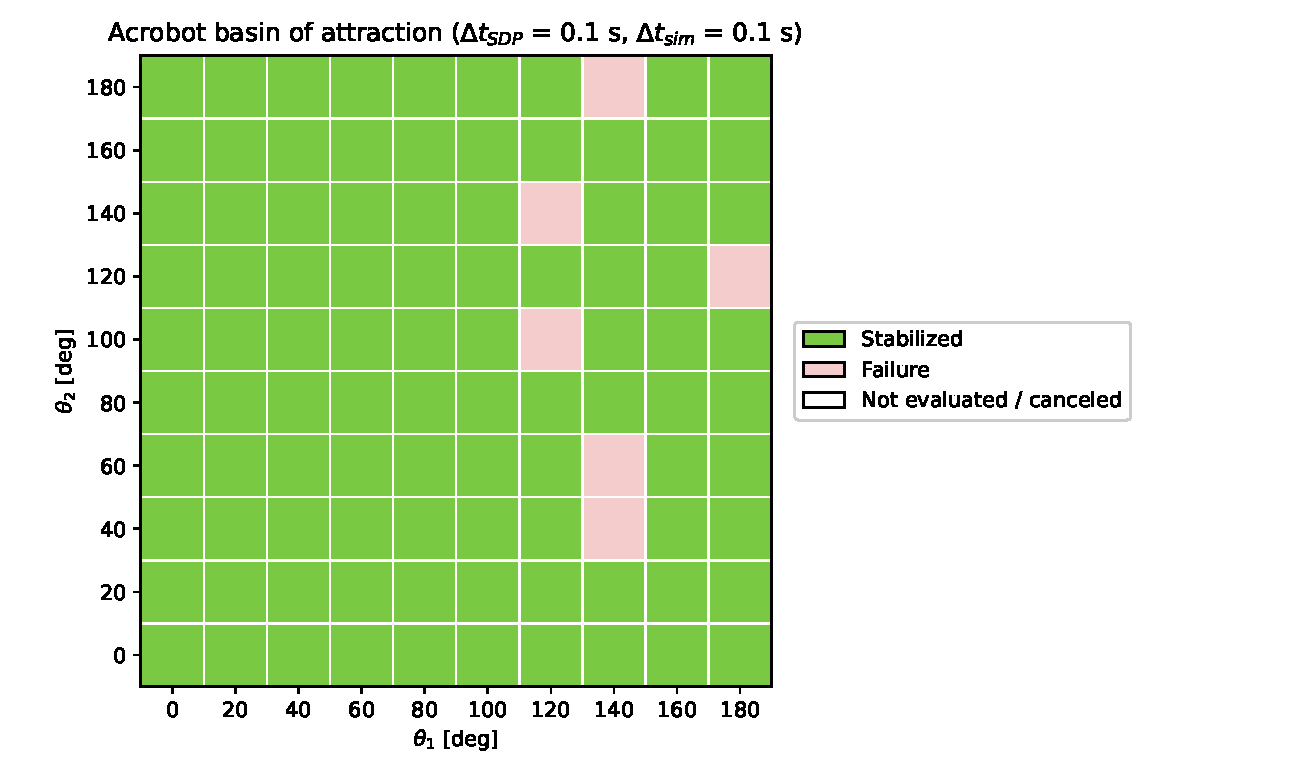
\includegraphics[width=\textwidth,trim=0 1.9cm 0 0,clip]{pics/Optimization/Acrobot/basin_of_attraction_01.pdf}
        \caption*{(a) Case~I.}
    \end{minipage}
    \hfill
    \begin{minipage}[t]{0.45\textwidth}
        \centering
        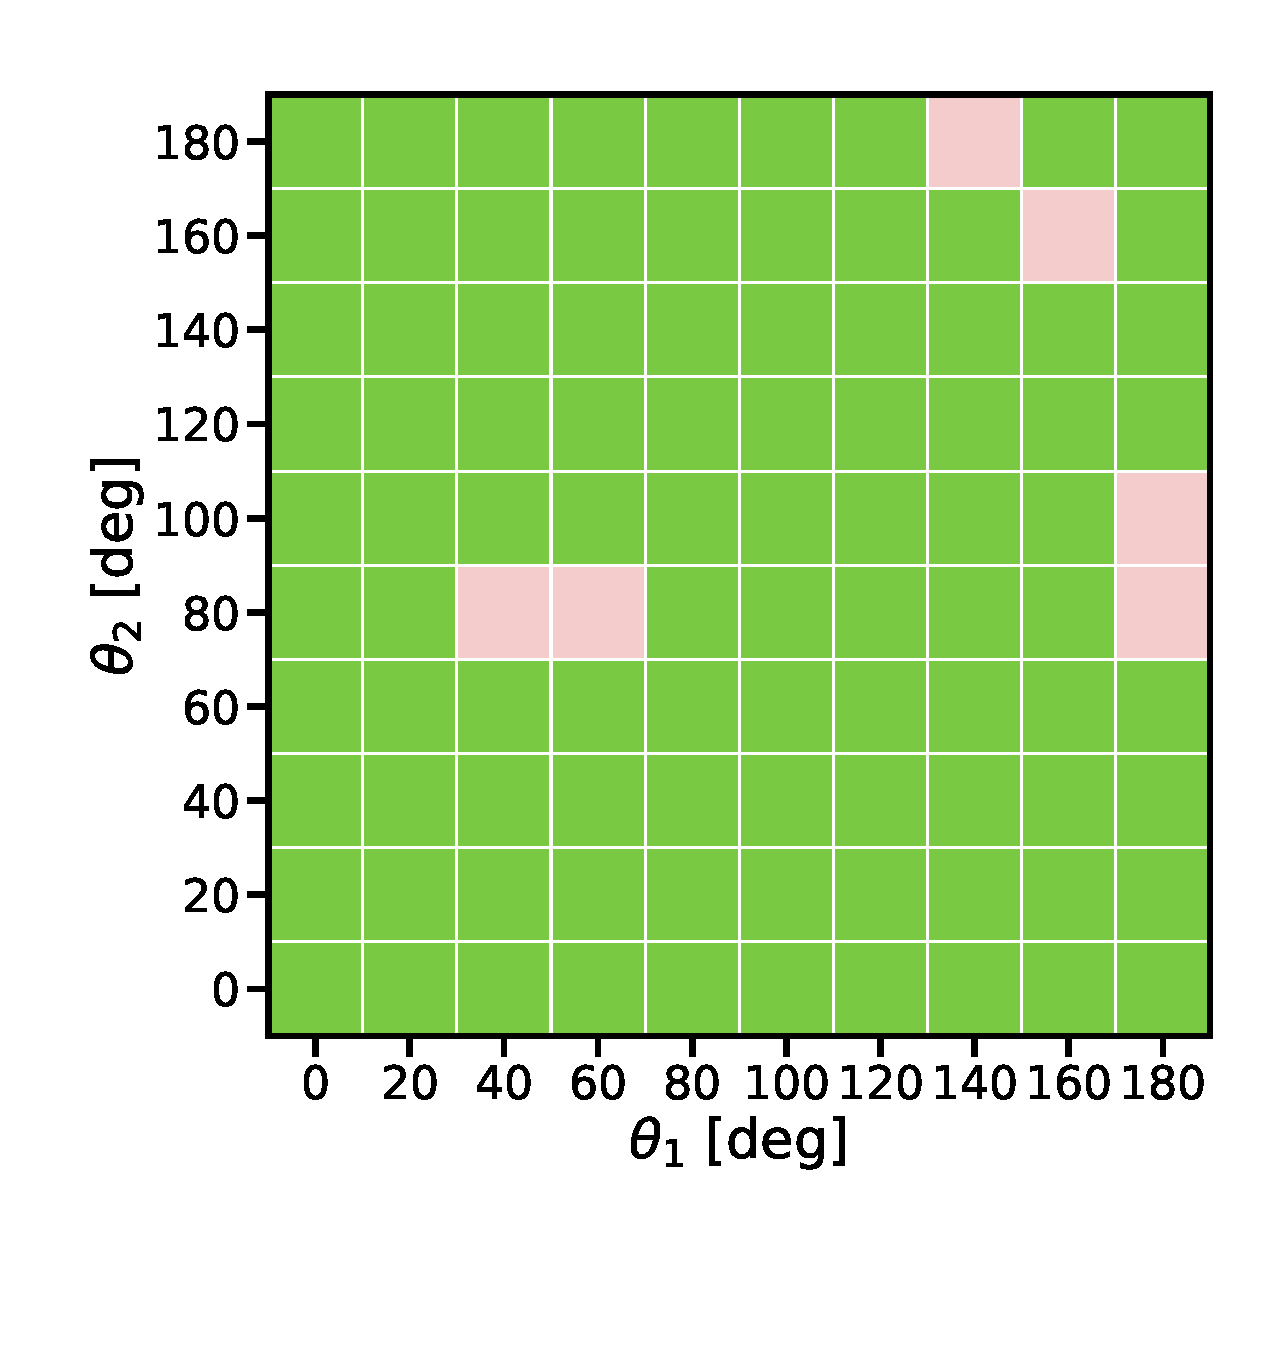
\includegraphics[width=\textwidth,trim=0 1.9cm 0 0,clip]{pics/Optimization/Acrobot/basin_of_attraction_005.pdf}
        \caption*{(b) Case~II.}
    \end{minipage}
    \par\medskip
    \begin{minipage}[t]{0.45\textwidth}
        \centering
        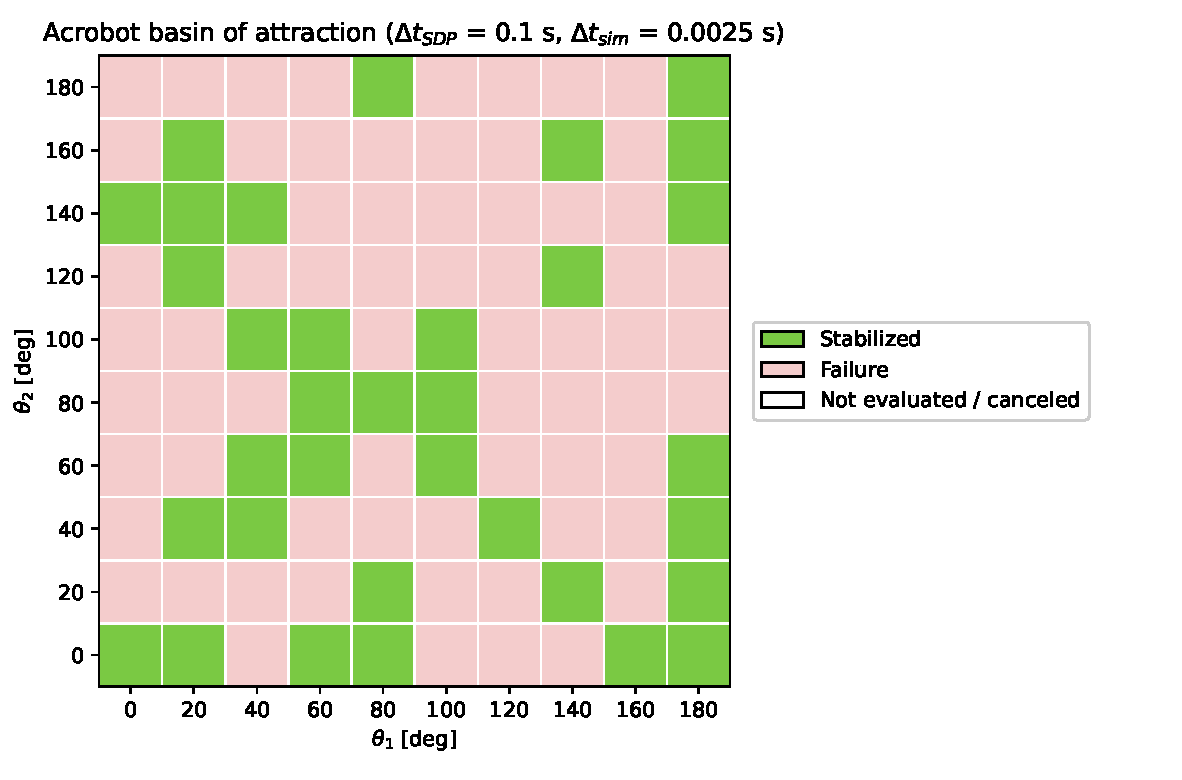
\includegraphics[width=\textwidth,trim=0 1.9cm 0 0,clip]{pics/Optimization/Acrobot/basin_of_attraction_00025.pdf}
        \caption*{(c) Case~III.}
    \end{minipage}

    \vspace{0.9\baselineskip}
    \caption{Empirical sampled stabilization regions of the SDP-MPC
    controller with $u_{\max}=15\,\mathrm{N\,m}$. The tuples
    $(\Delta t_{\mathrm{SDP}},\Delta t_{\mathrm{sim}},
    \Delta t_{\mathrm{ctrl}})$ are $(0.1,0.1,0.1)\,\mathrm{s}$ in Case~I,
    $(0.05,0.05,0.05)\,\mathrm{s}$ in Case~II, and
    $(0.1,0.0025,0.025)\,\mathrm{s}$ in Case~III.}
    \label{fig:acrobot_basin_comparison}
\end{figure}

Figures~\ref{fig:acrobot_basin_comparison} (a)-(b) show that the Acrobot 
model stabilizes $94$ of the $100$ 
initial configurations in Case~I. The matched time-scale configuration
of Case II also contains $94$ stabilized samples, although the locations
of the six non-stabilized entries changed. Therefore, reducing all three time steps
from $0.1\,\mathrm{s}$ to $0.05\,\mathrm{s}$ does not change the overall
stabilization success. Here, the failures occur
after the SDP optimization returns an infeasible solution. 

In contrast, only $34$ of the $100$ samples are marked as stabilized in
Case III, illustrated in Figure~\ref{fig:acrobot_basin_comparison} (c). 
The successful samples form a scattered set rather than a contiguous
region and occur primarily for easier configurations for 
$\theta_1 < 100^\circ$ or configurations 
in which link $i=1$ is already relatively close to the $180^\circ$ target. 
However, both groups are interrupted by failures. Moreover, only five of the thirty samples in the region
$120^\circ\leq\theta_1\leq160^\circ$ stabilize.
The increase in failure states cannot be explained only
by the smaller $\Delta t_{sim}$, as Case~II also refines
the prediction, simulation, and control intervals consistently, but without reducing
the total number of stabilized samples. Instead, the comparison between 
Case~I-II and Case~III indicates that 
the mismatched time scales in Case~III lead to increased failure rates. 
However, a possible case with 
$\Delta t_{SDP}=\Delta t_{sim}=\Delta t_{ctrl}=0.0025\,\mathrm{s}$
could not be evaluated due to the high computational cost of solving the SDP
problems with $N_{\mathrm{SDP}}=800$.

For the successfully stabilized initial configuration
$\theta_{1,\mathrm{init}}=\theta_{2,\mathrm{init}}=80^\circ$, the complete SDP-MPC 
computation required approximately $3.1\,\mathrm{h}$ in Case~I, $27.3\,\mathrm{h}$ in Case~II, 
and $17.8\,\mathrm{h}$ in Case~III. The runtime is determined first by $\Delta t_{\mathrm{SDP}}$ and 
$N_{\mathrm{SDP}}$, which define the size and cost of each SDP problem, and second by the time-discretization mismatch, 
which can increase the number of MPC iterations required before stabilization.

\begin{figure}[!t]
    \centering
    \begin{minipage}[t]{0.49\textwidth}
        \centering
        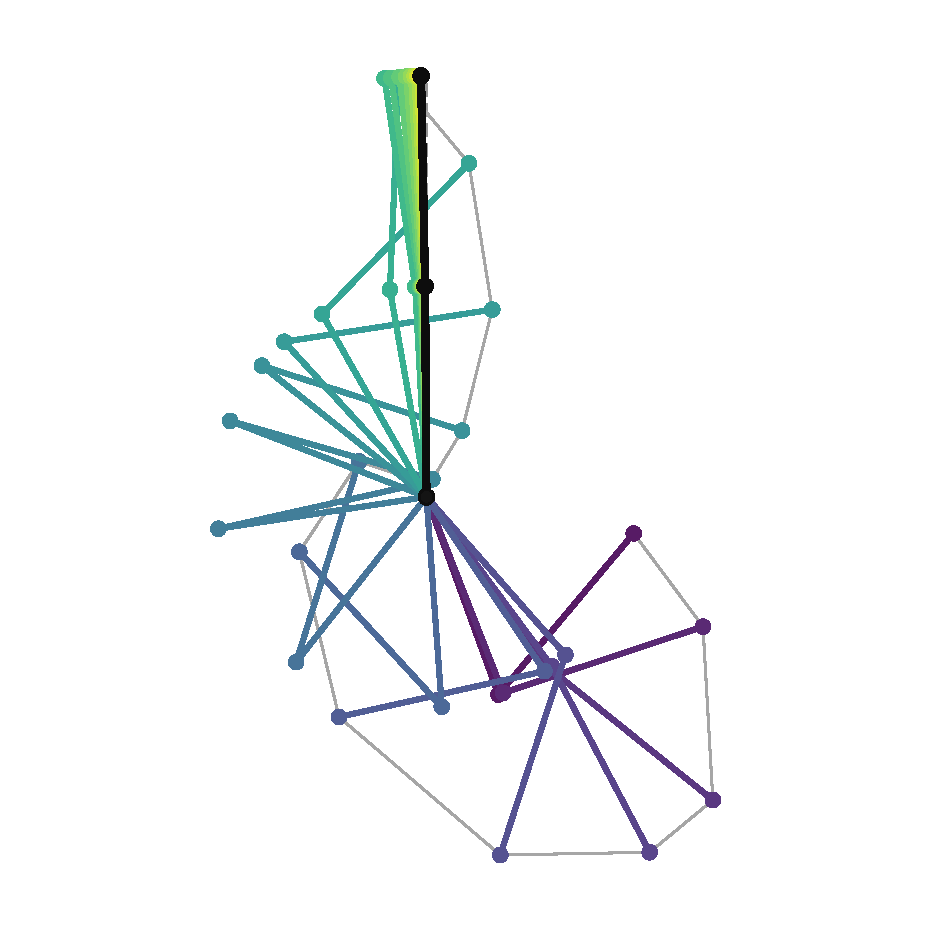
\includegraphics[width=\textwidth]{pics/Optimization/Acrobot/acrobot_trajectory_01_01_01.pdf}
        \caption*{(a) Case~I: $(0.1,0.1,0.1)\,\mathrm{s}$.}
    \end{minipage}
    \hfill
    \begin{minipage}[t]{0.49\textwidth}
        \centering
        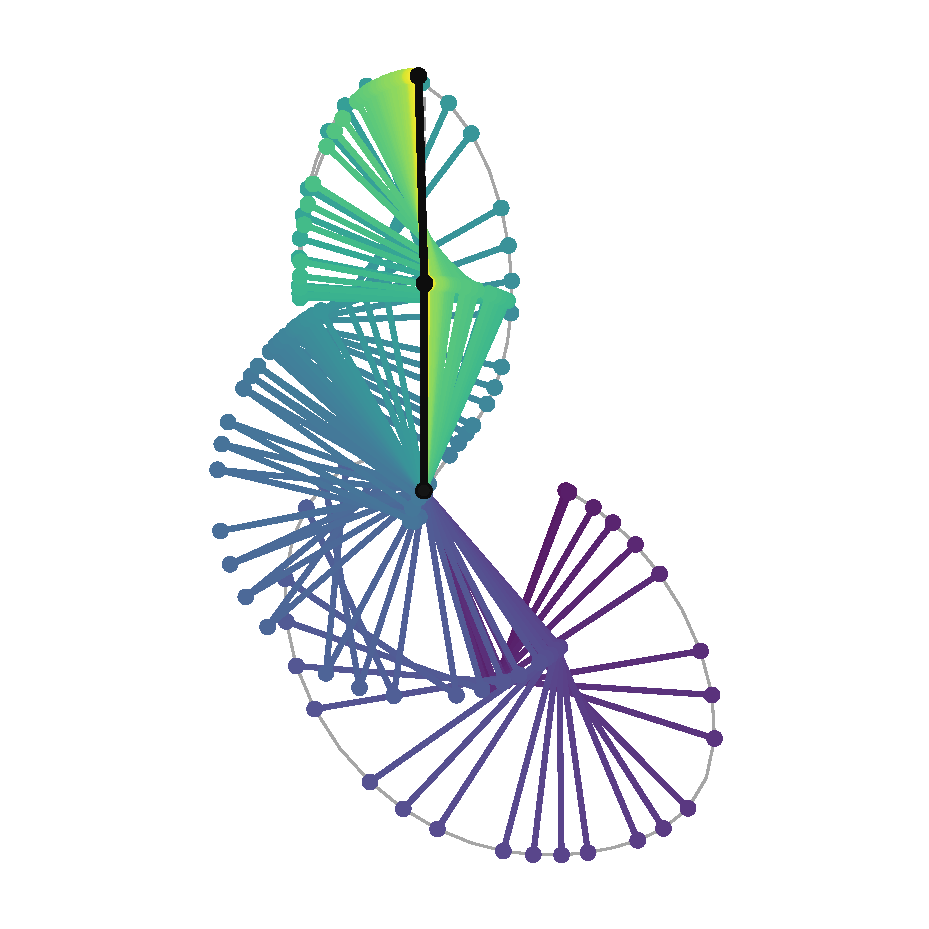
\includegraphics[width=\textwidth]{pics/Optimization/Acrobot/acrobot_trajectory_01_00025_0025.pdf}
        \caption*{(b) Case~III: $(0.1,0.0025,0.025)\,\mathrm{s}$.}
    \end{minipage}

    \caption{Closed-loop Acrobot tip trajectories and sampled link
    configurations for
    $(\theta_1^{\mathrm{init}},\theta_2^{\mathrm{init}})
    =(20^\circ,140^\circ)$ in Cases~I and III. Each tuple gives
    $(\Delta t_{\mathrm{SDP}},\Delta t_{\mathrm{sim}},
    \Delta t_{\mathrm{ctrl}})$.}
    \label{fig:acrobot_sampled_trajectory_comparison}
\end{figure}

The trajectory comparison in
Fig.~\ref{fig:acrobot_sampled_trajectory_comparison} illustrates the described
behaviour for the common initial configuration
$(\theta_1^{\mathrm{init}},\theta_2^{\mathrm{init}})
=(20^\circ,140^\circ)$. With matched $0.1\,\mathrm{s}$ time scales, the
Acrobot follows a comparatively direct swing-up and satisfies the stabilization
criterion after approximately $2.2\,\mathrm{s}$. The mismatched Case~III also
reaches the inverted equilibrium, but requires approximately $4.1\,\mathrm{s}$.
Its link-tip paths contain considerably larger loops, and the repeated passages
around the upright configuration indicate a more oscillatory transient. Thus,
receding-horizon feedback can compensate for the temporal mismatch in this
particular case, but only at the cost of a slower and less direct
closed-loop maneuver.

\paragraph{Summary}
For the evaluated initial states, the SDP-MPC controller can convert first-step
extractions into on-manifold simulated swing-ups, although the complete-horizon
moment relaxations are not generally numerically rank one. With
$u_{\max}=5\,\mathrm{N\,m}$, stabilization is obtained for the symmetric
$5^\circ$ initial state, but the limited control and unsuccessful additional
trials reveal limited control authority. Increasing the bound to
$15\,\mathrm{N\,m}$ yields broad sampled stabilization regions for matched
prediction and execution time scales, whereas the mismatched configuration
stabilizes only about one third of the tested initial states.
Although the SDP relaxations do not provide a certificate of global optimality, 
the results show that embedding the SDP optimization in a closed loop with numerical 
simulation can generate feasible stabilizing trajectories.




%\section{Experimental Results}

%A thesis almost always has an experimental part, typically some comparison to other approaches. Benchmarking takes time, for running the experiments, but also for thinking them up in the first place, and for analysing the results. Plan accordingly to spend enough time here!

%Think about what makes sense to measure, what you want to learn from your measurements. Think about what is really the relevant contribution of your thesis, and how you can prove that you have achieved your goals. Think about what you can measure in order to get a good insight into the performance of various aspects of your design, how you can distinguish between systematic and accidental effects, how you can convince yourself that your results are right. If you get surprising results, do not just say ``surprise, surprise, performance isn't as good as hoped''. Find out why. Surprises without explanation indicate either that you are clueless about what is going on, or that you have made a mistake. Unconvincing results, therefore, tend to imply unconvincing marks. 

%\paragraph{Statistics:} Measurements always have statistical (sampling) errors. Owing to the deterministic nature of simulations these are sometimes very small, as disturbing factors can be designed. However, the reader should be given an indication of how statistically significant the results are. This is done by providing at least a standard deviation in addition to averages. Whenever the results of several runs are averaged, a standard deviation can (and must) be supplied. After all, you average to reduce statistical errors.

%The reproducibility argument applies here just as much as for the implementation. Give enough detail on what you measure, and how you measure it, so that someone who has your implementation (but not your test code) or has re-done your implementation independently, should be able to repeat your measurements and arrive at essentially the same results. In some cases, results seem outright wrong in a thesis. In those cases, not enough detail is provided to allow the supervisor/reader to pinpoint the likely source of the error. Often the cause is systematic errors resulting from an incorrect measurement technique. If it seems wrong, and the text does not convince the reader that it is not wrong, the reader will assume that it is wrong.

\chapter{Discussion}
\label{chap:discussion}

Chapter \ref{chapter:evaluation} examined whether the proposed LGVI-SDP framework 
preserves the geometric structure
of the modeled rigid-body systems,
produces certifiable open-loop trajectories,
and can generate feasible trajectories for non-tight relaxations in a closed-loop implementation.
The results provide a qualified answer to the research question in Section \ref{sec:introduction_problem_statement}.
The framework is suitable for Lagrangian variational integrators of single- and multibody systems
and can certify particular discrete trajectory-optimization instances.
Still tightness, feasible extraction,
and computational cost depend strongly on the considered dynamics and remain challenging.
In the following, the main findings are discussed and related to the state of the art.
Finally, potential applications are elaborated.

\section{Discussion of Main Findings}
\label{sec:discussion_of_main_findings}
The simulation results in Section \ref{sec:numerical_simulation_results} 
establish that the derived discrete models of the 
3D pendulum on $\mathrm{SO}(3)$ and the underactuated Acrobot $(\mathrm{SO}(2) \times \mathbb{R}^2)^2$
represent the intended dynamics while exhibiting energy-conservation properties over a long time horizon.
For the unforced 3D pendulum,
Figure \ref{fig:simulation_results_3d_pendulum} shows that the LGVI remains on $\mathrm{SO}(3)$,
preserves the momentum
and exhibits bounded long-term energy error.
In comparison, a standard RK4 integrator has errors in all three quantities,
whereas projected RK4 restores the rotation constraint but accelerates energy drift.
The constrained Acrobot results in Figures \ref{fig:simulation_results_acrobot_unforced} 
and \ref{fig:simulation_results_acrobot_forced} extend this observation to a multibody system,
where both link rotations remain on $\mathrm{SO}(2)$,
the holonomic link constraints are satisfied,
and the unforced energy error remains bounded.
These results demonstrate that the derived discrete Lagrangian variational 
integrators of the 3D-pendulum \eqref{eq:forced_3D_pendulum_EL} and the 
Acrobot \eqref{eq:acrobot_full_del_shifted} preserve the relevant configuration 
and constraint geometry over the simulated horizon.


\paragraph{Single-body optimization}
The 3D pendulum demonstrates the complete method for a single rigid body.
Its LGVI can be written as the quadratic POP in \eqref{eq:controlled_3d_pendulum_pop},
but a dense second-order relaxation would already require a $91{,}378\times91{,}378$ 
moment matrix for $N=20$.
The minimum-degree chordal extension generated by SPOT in Section \ref{subsec:sparse_relaxations} 
reduces the largest matrix to $325\times325$,
compared with $820\times820$ for the complete temporal clique.
Therefore, the Moment-SOS relaxation can convert a nonconvex
algebraic LGVI formulation into a sparse convex optimization problem.
Still, the MD sparsity construction is required for computational application.

For all five targets $\theta_{x,des}=\{0^\circ, 45^\circ, 90^\circ, 135^\circ, 180^\circ\}$,
Table \ref{tab:pendulum_3d_sdp_statistics} reports a rank metric below $7.3\times10^{-8}$,
a manifold violation below $4.6\times10^{-8}$,
and a suboptimality gap below $1.8\times10^{-6}$.
Additionally, the solution extractions remain feasible.
Therefore, these values indicate that the second-order relaxations are numerically tight and
certify global optimality for the considered discrete POP.
Figure \ref{fig:optimization_results_x180_md} illustrates the $\theta_{x,des}=180^\circ$ case,
where the extracted trajectory reaches the desired attitude while remaining on $\mathrm{SO}(3)$.
Consequently, the single-body problem of a 3D pendulum on $SO(3)$ is globally certifiable 
using discrete LGVI dynamics and sparse SDP relaxations.

Still, it has to be noted that the certified solutions do not necessarily 
reach the desired states after exactly $N$ steps, while still being certifiable. For example,
the $\theta_{x,des}=90^\circ$ case reaches a terminal state of $\theta_{x,final}\approx70.5^\circ$,
since the implemented target is not a hard constraint but a cost inside the objective function.
Therefore, the certified solution is optimal for the discrete objective, 
but not for reaching the exact terminal state.

\paragraph{Multibody formulation and sparsity}
The Acrobot extends the framework to a constrained and underactuated multibody system.
Its maximal-coordinate LGVI represents both links separately
and imposes the joints through holonomic constraints and multipliers.
This enables a quadratic polynomial structure.
Moreover, the reduction introduced in Section \ref{sec:discrete_motion_planning_acrobot} eliminates 
the position variables and expresses the velocities through rotation variables.
Thereby, the size of the decision vector, which has to be optimized, 
decreases from $17N+3$ to $13N-1$ variables while preserving quadratic polynomial dynamics.
It therefore reduces the SDP without introducing densely coupled dynamical 
representations when using minimal coordinates \cite{BrudigamManchester2021LQR}.

Nevertheless, even after the reduction,
the dense second-order moment matrix has the dimension $304{,}590\times304{,}590$ for $N=60$.
The complete chain-like sparsity construction \eqref{eq:acrobot_full_self_initial_clique}-
\eqref{eq:acrobot_full_self_interior_cliques} replaces the dense 
matrix with separate blocks of sizes $351\times351$ and $253\times253$.
The multibody-specific construction in \eqref{eq:acrobot_hybrid_self_cliques} 
keeps the complete cliques at $k=1,2$,
but separates later dynamics and kinematics into $171\times171$ and $91\times91$ matrices.
The results of the SDP relaxation, shown in Tables \ref{tab:acrobot_sdp_statistics_full} and
\ref{tab:acrobot_sdp_statistics_hybrid},
identify similar relaxation metrics for both structures.
Still, the specialized cliques reduce the MOSEK runtime by a factor of approximately three to five.
Consequently, the identification of problem-specific sparsity is necessary 
for solving multi-body systems using semidefinite programming to obtain 
fast and numerically reliable results \cite{Kang_2025Global}. 

However, it is important to note that multibody-specific sparsity does not guarantee tighter relaxations 
than chain-like sparsity. Therefore, before applying the proposed framework to new multibody systems, 
it is necessary to evaluate the tightness of the relaxation for the specific problem.

\paragraph{Open-loop Acrobot optimization}
The open-loop SDP evaluation in Section \ref{subsec:acrobot_optimization_results} 
separates easy from difficult Acrobot problems.
For the targets $\theta_{\mathrm A}^{\mathrm{des}}=0^\circ$ and
$\theta_{\mathrm A}^{\mathrm{des}}=45^\circ$,
Tables \ref{tab:acrobot_sdp_statistics_full} and \ref{tab:acrobot_sdp_statistics_hybrid} report 
rank-one moment matrices, feasible extractions, and negligible suboptimality gaps.
Therefore, in these cases, the solutions are certified.
However, similar to the 3D-Pendulum, the certified $45^\circ$ solution retains a terminal 
error of approximately $55^\circ$, because the target is only weighted in the objective.

For the targets $\theta_{\mathrm A}^{\mathrm{des}}=90^\circ$,
$\theta_{\mathrm A}^{\mathrm{des}}=135^\circ$, and
$\theta_{\mathrm A}^{\mathrm{des}}=180^\circ$,
the maximum rank metric increases to approximately $0.35$-$0.66$,
while the extracted rotations have manifold violations around $1.0$-$1.4$.
Therefore, the first moments do not define feasible $\mathrm{SO}(2)$ trajectories
and no certificate is obtained. The results indicate that the additional complexity of the multibody
underactuated system increases the difficulty of the convex optimization problem.

For the runtime, the optimization using specialized multibody cliques \eqref{eq:acrobot_hybrid_self_cliques} 
requires approximately $15$-$31$ minutes,
compared with $45$-$113$ minutes for the chain-like cliques \eqref{eq:acrobot_full_self_initial_clique}-
\eqref{eq:acrobot_full_self_interior_cliques}.
Therefore, this demonstrates that the size of the moment matrices is the driving factor for the runtime of the SDP solver.
Still, both optimization variants remain too slow for online control.
A lower relaxation order would reduce matrix sizes but weaken the tightness of the relaxation.
Moreover, instead of using the second order interior-point solver MOSEK \cite{MOSEK}, 
a first-order SDP solver, for example CuADMM \cite{Kang_2026Fast}, could accelerate the same relaxation
at the possible cost of less accurate certified solutions. Additionally, in this thesis, only 
second order $\kappa = 2$ relaxations are considered, as \cite{Sangli2025}
states that second order relaxations are sufficient for most of the considered problems. In general, 
higher order relaxations can be used to tighten the relaxation \eqref{eq:convergence_of_moment_sos_hierarchy}, 
but at the cost of increased computational complexity.

\paragraph{Closed-loop Acrobot stabilization}
Tables \ref{tab:acrobot_sdp_statistics_full} and \ref{tab:acrobot_sdp_statistics_hybrid} 
show that $\delta_1$ is smaller than the worst-horizon metric $\delta_{\max}$ inside 
the open-loop optimization.
This motivates the receding-horizon implementation in Section 
\ref{sec:acrobot_trajectory_optimization_SDP_MPC}, where
only the first control from \eqref{eq:acrobot_mpc_applied_control} is applied.
The remaining non-tight prediction is discarded,
and the SDP is solved again from the simulated state.
However, $\delta_1$ is not a rank-one condition and therefore not tight.
Still, the implemented closed-loop control has a feedback structure, 
which can stabilize the system even if the open-loop solution is not tight 
(see Section \ref{subsec:acrobot_sdp_mpc_results}).

Figure \ref{fig:acrobot_mpc_u5_closed_loop} 
illustrates that this procedure stabilizes the system starting from an initial rotation of $5^\circ$,
after approximately $11.9\,\mathrm{s}$ with $u_{\max}=5\,\mathrm{N\,m}$.
The simulated trajectory remains on $\mathrm{SO}(2)$
although the predicted blocks are not rank one throughout the whole maneuver.
This demonstrates numerical closed-loop feasibility for the tested configuration.
However, the solution cannot be considered globally optimal, since the 
optimization problem is not tight. Additionally, failures are also 
consistent with limited control torque availability for $u_{\max}=5\,\mathrm{N\,m}$.

With $u_{\max}=15\,\mathrm{N\,m}$,
Figure \ref{fig:acrobot_basin_comparison} 
shows that the matched discretization ($\Delta t_{SDP} = \Delta t_{\mathrm{sim}}= \Delta t_{ctrl}$) 
Cases~I and~II stabilize $94$ of $100$ initial configurations.
Therefore, consistently refining all $\Delta t_{SDP}$ and $\Delta t_{\mathrm{sim}}$ intervals from $0.1\,\mathrm{s}$ to $0.05\,\mathrm{s}$
does not change the success rate. Nevertheless,
the different failed trials for the same initial conditions between Cases~I and~II
indicate that the success is not guaranteed for all $\Delta t_{SDP} = \Delta t_{\mathrm{sim}}= \Delta t_{ctrl}$
configurations.

In Case~III, where there is a discretization mismatch 
between the SDP and simulation time steps
($\Delta t_{SDP} = 0.1\,\mathrm{s}$, 
 $\Delta t_{\mathrm{sim}}= 0.0025\,\mathrm{s}$, $\Delta t_{ctrl} = 0.025\,\mathrm{s}$),
the controller stabilizes only $34$ of $100$ configurations.
Consequently, Figure \ref{fig:acrobot_sampled_trajectory_comparison}(b) shows a more oscillatory behaviour
near the target configuration before stabilization, compared to
Case~I in Figure \ref{fig:acrobot_sampled_trajectory_comparison}(a) for the same initial condition of $(\theta_1^{\mathrm{init}},\theta_2^{\mathrm{init}})=(20^\circ,140^\circ)$.
Here, Case~III requires $4.1\,\mathrm{s}$
instead of $2.2\,\mathrm{s}$ in Case~I.
The results indicate that mismatched discretization can lead to 
reduced reliability for stabilization of the Acrobot.

For the successful $(\theta_1^{\mathrm{init}},\theta_2^{\mathrm{init}})=(80^\circ,80^\circ)$ example,
Cases~I, II, and III require approximately $3.1\,\mathrm{h}$,
$27.3\,\mathrm{h}$,
and $17.8\,\mathrm{h}$.
These illustrative runtimes depend on $\Delta t_{\mathrm{SDP}}$ and $N_{\mathrm{SDP}}$,
which determine each SDP size,
and on the number of replanning iterations.
A matched discretization case with $\Delta t_{\mathrm{SDP}} =\Delta t_{\mathrm{sim}}=\Delta t_{\mathrm{ctrl}}=0.0025\,\mathrm{s}$ 
would require $N_{\mathrm{SDP}}=800$, which is not computationally feasible with current hardware.
Consequently, the closed-loop implementation is only considered as an offline application 
instead of a real-time controller. However, the 
open-loop optimization using semidefinite relaxation is also not real-time capable, since the SDP solver requires
approximately $15$-$31$ minutes for the considered $N_{\mathrm{SDP}}=60$ problem.

\section{Comparison with the State of the Art}
\label{sec:comparison_state_of_the_art}

The first contribution of this thesis is the Acrobot-specific LGVI in maximal coordinates
\eqref{eq:acrobot_full_del_shifted}, including its underactuation
\eqref{eq:forced_acrobot_rotational_equations} and holonomic joint constraints. This formulation aligns with
the preservation properties of
\cite{Marsden2001,Lee2008} and the maximal-coordinate formulations in
\cite{BrudigamManchester2021VariationalIntegrators,BrudigamManchester2021LQR}.
Moreover, the reduction in Section \ref{sec:discrete_motion_planning_acrobot}
resulted in a smaller decision vector $\bm{z}$ and a
quadratic polynomial model suitable for SDP relaxation \eqref{eq:controlled_acrobot_pop}.

The closest framework to this thesis is \cite{Sangli2025}. In that work, all reported 
trajectories are passed through a local-search step using IPOPT, including cases for which 
the SDP relaxation provides a small optimality gap or satisfies the rank condition. 
In contrast, the second-order relaxations of all considered 3D-pendulum problems in this 
thesis are numerically rank one and directly yield feasible trajectories without subsequent 
NLP refinement. The agreement between the SDP lower bound and the objective of the extracted 
trajectory therefore certifies global optimality using the SDP solution alone. This 
demonstrates that, for the investigated single-body benchmark, the complete pipeline from the 
nonconvex LGVI formulation to a feasible and globally optimal trajectory can be performed 
without depending on the initialization or convergence of a local solver, in contrast to \cite{Sangli2025}. 
Nevertheless, the drone problems in 
\cite{Sangli2025} include translational dynamics and obstacle avoidance and are therefore 
more complex than the present pendulum problem. Whether similarly direct SDP extraction 
remains possible after introducing obstacle constraints for the 3D-pendulum 
has to be evaluated in future research.
%%%%%%%%%%%%%%%
With respect to the research gap identified in Section~\ref{sec:introduction_research_gap}, this thesis 
demonstrates that the complete LGVI-SDP framework can be transferred from a single rigid body 
to a constrained and underactuated multibody system of increased dynamical complexity. 
The results confirm that globally optimal trajectories can be 
certified when the relaxation is tight and that closed-loop feedback controls can still be 
extracted for some non-tight problems, for example the Acrobot stabilization. 
However, the transfer is not equally reliable for 
all configurations, since relaxation tightness, solver feasibility, and computational cost 
remain strongly problem-dependent. In particular, the closed-loop trajectories do not 
provide certificates of global optimality, and their computation is 
too slow for real-time application. The research gap is therefore addressed for the 
investigated single- and multibody models, but remains open for larger systems, contact 
and obstacle constraints, uncertain dynamics, and hardware experiments.


\section{Potential Applications}
\label{sec:potential_applications}

The most direct application is offline trajectory generation. Tight SDP solutions
can provide certified benchmarks for evaluating local optimizers, as initial guesses 
for related NLP problems, 
or as reference trajectories for online tracking controllers.

For non-tight problems, the SDP-MPC implementation can still generate feasible
realized trajectories. The resulting state-control sequences could
be stored as demonstrations for faster online MPC methods or used to construct
warm starts from previously solved configurations. This is consistent with
\cite{Kang_2026Fast}, where data-based warm starts substantially reduce repeated
SDP solution times.

The trajectories could also provide training data for imitation learning or
offline reinforcement learning. This is particularly relevant for underactuated
systems such as the Acrobot, where swing-up requires coordinated actions over a
longer time horizon and can be difficult to explore \cite{acrobot_RL}.
A learned controller could approximate the SDP closed-loop policy while operating
at lower online cost.

%_____Zusammenfassung, Ausblick_________________________________
\chapter{Conclusion}
\label{chap:conclusion}

This thesis analyzed the combination of Lie group
variational integrators (LGVIs) with sparse Moment-SOS semidefinite relaxations
for multi rigid-body trajectory optimization. 

Firstly, Chapter \ref{sec:introduction} 
formulated the general optimization problem and identified the research gap of 
semidefinite relaxation providing global optimal solutions
for some low-dimensional rigid-body systems, however, not analyzed for 
different complex multibody systems.
Thereby, accuracy of lower bounds, relaxation tightness and feasible extraction become
problem dependent as the dynamical complexity increases. This question was
examined for a single rigid body and a constrained, underactuated multibody
system.

In order to derive LGVIs, 
Chapter \ref{chapter:preliminaries_lie_groups} briefly introduced the matrix 
Lie groups, Lie algebras, and local
group variations required for the following derivations.
%%%%%%

Chapter \ref{chapter:continous_mechanics_of_rigid_bodies_on_lie_groups} 
established the continuous mechanical foundation. The
Euler-Lagrange equations on a matrix Lie group were derived from Hamilton's
principle using left-trivialized variations \eqref{eq:continuous_euler_lagrange_lie_group}.
Additionally, the Legendre transformation was
used to express the dynamics in Hamiltonian form \eqref{eq:continuous_hamilton_equations_lie_group}. 
This framework was applied to
the unforced 3D pendulum on $\mathrm{SO}(3)$, for which the continuous equations
were derived \eqref{eq:continuous_3D_pendulum_euler_lagrange}. 
To validate the LGVI properties of the 3D pendulum,
the momentum conservation associated with rotations about gravity was
verified \eqref{eq:continuous_3d_pendulum_validation} using Noether's theorem.

Afterwards, Chapter \ref{chapter:discrete_mechanics_for_rigid_bodies_on_lie_groups} 
transferred the continous lagrangian variational construction to discrete time. 
Instead of
discretizing the continuous equations of motion directly, the action integral was
replaced by a discrete action sum \eqref{eq:discrete_action_sum}. 
This yields to the discrete Euler-Lagrange \eqref{eq:discrete_euler_lagrange_lie_group} 
and Hamiltonian equations \eqref{eq:discrete_hamilton_equations_lie_group}, 
discrete Legendre transformations \eqref{eq:discrete_legendre_transformations}, 
and their forced extension \eqref{eq:discrete_forced_Euler_Lagrange}. 
A computational approach was introduced to solve the implicit discrete equations of motion. 
Thereby, multiplicative kinematic updates preserve the Lie-group structure, 
while a Cayley parametrization and Newton iteration solved the implicit rotation 
update. In corespondance, to the continous case, the discrete 
unforced and controlled 3D-pendulum LGVI were derived \eqref{eq:discrete_3D_pendulum_EL}. 
This single rigid-body formulation was
extended to a multi-body framework for deriving LGVI for coupled rigid bodies. 
Therefore, the Acrobot LGVI using maximal coordinates was derived as an example 
\eqref{eq:acrobot_full_del_shifted}. Its two center-of-mass positions and
$\mathrm{SO}(2)$ attitudes were coupled by holonomic constraints and
Lagrangian multipliers.

To optimize these models trajectories, Chapter \ref{chapter:certifiable_trajectory_optimization} 
transforms these discrete dynamical models into finite-horizon polynomial
optimization problems (POPs). However, as these equations are nonconvex
semidefinite programming is introduced to convert these into convex optimization problems.
Thereby the Moment-SOS hierarchy and sparse relaxations are introduced. 
Afterwards, the POP of the 3D-pendulum is defined on
$\mathrm{SO}(3)$ \eqref{eq:controlled_3d_pendulum_pop}. 
For the Acrobot, the derived LGVI was reduced to a smaller variable size optimization problem.
Thereby, the holonomic constraints eliminated
the positions and the velocity variables, which were expressed through rotations, 
reducing the decision vector from $17N+3$ to $13N-1$ variables. Still, 
the quadratic structure of the dynamics was preserved. The resulting POP was defined in \eqref{eq:controlled_acrobot_pop}.
In addition, chain-like cliques \eqref{eq:acrobot_full_self_interior_cliques} 
were compared with a multibody-specific
clique construction \eqref{eq:acrobot_hybrid_self_cliques} 
to seperate moment matrices for computational efficiency.
Finally, the reduced Acrobot POP was embedded in an SDP-based
model predictive control (MPC) loop that applied only the first extracted control
after each SDP optimization itteratively.

In Consequence, Chapter \ref{chapter:evaluation} 
evaluated the resulting models and optimization problems. 
Firstly, a numerical simulation of the 3D-pendulum LGVI 
and the Acrobot LGVI was implemented to verify the derived equations of motion.
As result, the unforced 3D-pendulum simulation remained on $\mathrm{SO}(3)$, 
preserved the momentum, and conserved the energy over a long time horizon. 
Similarly, the Acrobot simulations preserved both $\mathrm{SO}(2)$ attitudes and 
the base and elbow constraints. 
Secondly, the POPs were solved using SDP relaxations and evaluated for 
feasibility and optimality. All five evaluated 3D-pendulum relaxations 
were numerically rank one, gave feasible extractions, and were certified for 
their discrete POPs (see Table \ref{tab:pendulum_3d_sdp_statistics}). 
For the 3D-pendulum minimum degree chordal extension
was used for the clique construction. Moreover, the Acrobot $0^\circ$ and $45^\circ$ targets were also 
certified using chain-like cliques and multibody-specific clique constructions. 
In contrast, the $90^\circ$,
$135^\circ$, and $180^\circ$ semidefinite relaxation cases produced higher-rank moment
matrices and infeasible extractions (see Table \ref{tab:acrobot_sdp_statistics_full}-\ref{tab:acrobot_sdp_statistics_hybrid}). 
Therefore, no global certificate was obtained for these cases. Nevertheless,
the closed loop MPC implementation with repeated
first-control extraction generated feasible simulated Acrobot swing-ups. With
the $15\,\mathrm{N\,m}$ bound, the two matched time-scale cases each stabilized
$94$ of $100$ sampled states, compared with $34$ of $100$ for the mismatched
case (see Fig.\ref{fig:acrobot_basin_comparison}). 

Finally, Chapter \ref{chap:discussion} interpreted these findings in relation to the research question and
the state of the art literature. Additional, possible applications of optimization and learning-based methods were identified.

In connection to the research question the results provide following analysis. 
The LGVI
dynamics of both considered systems can be represented by low-degree polynomial
constraints while retaining their Lie-group structure. The resulting POPs can be solved by sparse Moment-SOS relaxations, 
which can provide certified global optima for some low-dimensional
rigid-body problems. Here, Sparse second-order Moment-SOS relaxation recovered feasible trajectories that
were certified as globally optimal for the tight 3D-pendulum problems and the two
simpler Acrobot optimization problems. However, the Acrobot cases of 
$\theta_{des} \geq 90^\circ$ prevent this result from being
generalized to complex multibody motions. 
Also, sparsity reduces the SDP computation time, 
but does not guarantee tightness or feasible extraction.
The approach of an closed-loop SDP-MPC produces feasible trajectories 
for even complex optimization problems, for example the stabilization of 
an underactuated Acrobot,
when the prediction was not rank one. However, it did not globally certify 
these solutions.

\paragraph{Limitations}

This thesis does not consider contact, collision avoidance and obstacles. Adittionally,
hardware experiments were not performed.

Computational scaling is the strongest practical limitation because the moment
matrix dimension grows with the variables in each clique. Without
sparsity, the reported problems would require matrices of size
$91{,}378\times91{,}378$ and $304{,}590\times304{,}590$. Even with sparsity,
MOSEK required about $56$ to $69$ min for one 3D-pendulum problem,
$15$--$31$ min for the special-multibody Acrobot cliques, and $45$--$113$ min
for the complete chain-like cliques on eight CPU cores. The successful initial
$(80^\circ,80^\circ)$ Acrobot MPC computations required $3.1$, $27.3$, and $17.8$ hours
in Cases I--III. The implementation is therefore an offline study. In general, larger
time horizons, systems, or coupled constraints are increasing the computational
expense significantly.

\paragraph{Future Work}

A first direction is to reduce the polynomial representation before constructing
the SDP. For spatial rotations, a unit-quaternion formulation should be compared
with the rotation-matrix formulation used here. The relevant question is not only
whether fewer scalar attitude variables are obtained, but whether the complete
quaternion POP produces smaller sparse moment blocks while preserving suitable
polynomial dynamics and reliable extraction. This comparison should include the
resulting polynomial degree, constraints, clique structure, numerical conditioning,
and relaxation tightness.

The framework should next be transferred to additional multibody benchmarks. A
cart--pole system provides a useful intermediate problem containing translational
and rotational motion. Its LGVI and reduced POP could be derived, its temporal
and problem-specific sparsity identified, and the generic and user-defined clique
constructions compared. The same SDP--MPC procedure could then be applied to
determine whether the first-control strategy remains effective. This would provide
a controlled progression toward systems with more links, followed by obstacle,
contact, uncertainty, and hardware experiments already identified as open in this
thesis.

The computational backend should also be reconsidered. A first-order GPU solver
such as CuADMM could replace the interior-point solver MOSEK and substantially
reduce solution time, although potentially lower numerical accuracy
would have to be evaluated carefully whenever a certificate is claimed. The solver
itself would not make a fixed relaxation tighter. However, faster solution of the
SDP could make larger cliques or higher relaxation orders affordable, which may
yield tighter bounds for the difficult Acrobot cases, and could reduce the cost of
longer horizons. Warm starting consecutive MPC problems and reusing their
unchanged polynomial and sparsity structure should be investigated for the same
reason.

Finally, future work could examine adaptive and iterative extraction. Rank metrics
could identify locally tight moment blocks, after which only variables supported by
verified rank-one blocks would be fixed and the remaining relaxation solved again.
Clique merging or a higher relaxation order could be applied selectively where the
rank condition fails. Such a procedure may help construct a feasible full-horizon
trajectory, but fixing local decisions alone is not a certificate of global optimality.
A global claim would still require satisfaction of all constraints of the original POP
and agreement between the objective of the completed feasible trajectory and a
valid lower bound for that original problem. In parallel, hard terminal constraints
or terminal sets should be evaluated so that certification refers to reaching the
target rather than only minimizing a soft tracking cost. For the closed-loop method,
a systematic study of matched prediction and execution time scales, together with
terminal stability conditions, would be required before extending the approach
from empirical stabilization to a certified controller.


\begin{comment}
	
Do not just leave it at the discussion: discuss what you/the reader can learn from the results. Draw some real conclusions. Separate discussion/interpretation of the results clearly from the conclusions you draw from them. (So-called ``conclusion creep'' tends to upset reviewers. It means surrendering your scientific objectivity.) Identify all shortcomings/limitations of your work, and discuss how they could be fixed (``future work''). It is not a sign of weakness of your work if you clearly analyze and state the limitations. Informed readers will notice them anyway and draw their own conclusions if not addressed properly.

\vspace{\baselineskip}
Recap: do not stick to this structure at all cost. Also, remember that the thesis must be:

\begin{itemize}
	\item honest, stating clearly all limitations
	\item self--contained, do not write just for the locals, do not assume that the reader has read the same literature as you, do not let the reader work out the details for themselves
\end{itemize}

This chapter is followed by the list of figures and the bibliography. If you are using acronyms, listing them (with the expanded full name) before the bibliography is also a good idea. The acronyms package helps with consistency and an automatic listing.
\end{comment}



%%%%%%%%%%%%%%%%%%%%%%%%%%%%%%%%%%%%%%%%%%%%%%%%%%%%%%%%%%%%%%%
%%%%%%%%%%%%%%%%%%%%%%%% Appendix %%%%%%%%%%%%%%%%%%%%%%%%%%%%%
%%%%%%%%%%%%%%%%%%%%%%%%%%%%%%%%%%%%%%%%%%%%%%%%%%%%%%%%%%%%%%%
\appendix

% Add optional appendix here
%_________Appendix__________________________________

% final tutorial remarks
\ifLSRITRtutorial
	\chapter{BUSTED! Last chance to actually read the HowTo-Section!}
	
%	Make sure your thesis is well structured, that each major section does what it is supposed to do, and that the whole thing hangs together. The basic structure is often as given in this template (but other structures are possible). In particular, don't think you need to have exactly as many major sections or chapters as the list implies; sometimes it makes sense to merge things, sometimes it makes sense to move things (e.g., the literature review is in many papers deferred until after the results), sometimes it makes sense to split a logical part into several individual sections. Just use some common sense.
%	
%	Hand in your thesis at minimum \textbf{one week} before the deadline for correction. You will receive feedback for the final version and very likely have to do minor or major revisions of your writing. Plan your writing schedule to allow for these adjustments, which can have quite some impact on your grade! 
%	
%	\optional{Please have a look on our \href{https://wiki.lsr.ei.tum.de/thesiswriting_students}{thesis-guidelines} as well before submitting your \emph{final} thesis.}
	
\optional{Do not forget to check our \href{https://wiki.tum.de/display/lsritr/Students}{\underline{thesis-guidelines}} before submitting your \emph{final} thesis.}	
	
%	\section{Style and Expressions}
%	
%	Before handing in your thesis, even for an intermediate review, please perform a spellcheck and correct grammar mistakes. The report is not meant to be a narrative text. Please stick to neutral and technical style and avoid subjective or biased expressions or adjectives/adverbs such as \emph{obviously, always, very, especially well, actually, so-called etc}. Scientific writing is about precision and you should underpin your statements factually, not soften them with unnecessary qualifiers.
%	
%	... Okay enough. But please check chapter \ref{sec:Tutorial} before starting with your report. 

\paragraph{Spellcheck reminder}
Before handing in your thesis, even for an intermediate review, please perform a proper spellcheck and correct grammar mistakes. Otherwise, there is a high likelihood that your supervisor will return your report immediately without making any comments.
\fi


\chapter{Scalar Implementation of POPs}
% Insert this chapter after \appendix in the main thesis file.
\section{Scalar Implementation of the 3D-Pendulum Optimization Problem}
\label{app:controlled_3d_pendulum_scalar_pop}

This appendix expands the matrix formulation
\eqref{eq:controlled_3d_pendulum_pop} into the scalar polynomial equations used
to construct the semidefinite relaxation. Let
\begin{equation}
R_k=[r_{ij,k}]_{i,j=1}^{3},
\qquad
F_k=[f_{ij,k}]_{i,j=1}^{3},
\qquad
J_d=\operatorname{diag}(\delta_1,\delta_2,\delta_3),
\label{eq:app_3d_scalar_matrices}
\end{equation}
and define
\begin{equation}
\rho_c=
\begin{bmatrix}\rho_1&\rho_2&\rho_3\end{bmatrix}^{\top},
\qquad
\bar u_{p,k}=
\begin{bmatrix}\bar u_{p1,k}&\bar u_{p2,k}&\bar u_{p3,k}\end{bmatrix}^{\top},
\qquad
u_{p,k}=u_{\max}\bar u_{p,k}.
\label{eq:app_3d_scalar_vectors}
\end{equation}

\paragraph{Objective and Discrete Dynamics}

Writing \(R_N^{\mathrm{des}}=[r_{ij,N}^{\mathrm{des}}]\) and
\(F^{\mathrm{des}}=[f_{ij}^{\mathrm{des}}]\), the scalar objective is
\begin{align}
J
=\;&
\rho_R\sum_{i=1}^{3}\sum_{j=1}^{3}
\left(r_{ij,N}-r_{ij,N}^{\mathrm{des}}\right)^2
+\rho_F\sum_{i=1}^{3}\sum_{j=1}^{3}
\left(f_{ij,N-1}-f_{ij}^{\mathrm{des}}\right)^2
\notag\\
&+\sum_{k=0}^{N-1}\alpha_R
\sum_{i=1}^{3}\sum_{j=1}^{3}
\left(r_{ij,k}-r_{ij,N}^{\mathrm{des}}\right)^2
\notag\\
&+\sum_{k=0}^{N-2}\alpha_F
\sum_{i=1}^{3}\sum_{j=1}^{3}
\left(f_{ij,k}-f_{ij}^{\mathrm{des}}\right)^2
\notag\\
&+\sum_{k=1}^{N-1}\gamma^{-1}
\left(\bar u_{p1,k}^2+\bar u_{p2,k}^2+\bar u_{p3,k}^2\right).
\label{eq:app_3d_scalar_objective}
\end{align}

Since \(R_k^{\top}e_3=[r_{31,k}\;r_{32,k}\;r_{33,k}]^{\top}\), write the
gravity moment as
\[
\tau_{g,k}=
\begin{bmatrix}\tau_{g1,k}&\tau_{g2,k}&\tau_{g3,k}\end{bmatrix}^{\top}.
\]
Its components are
\begin{subequations}
\label{eq:app_3d_scalar_gravity}
\begin{align}
\tau_{g1,k}&=mg\left(\rho_2r_{33,k}-\rho_3r_{32,k}\right),\\
\tau_{g2,k}&=mg\left(\rho_3r_{31,k}-\rho_1r_{33,k}\right),\\
\tau_{g3,k}&=mg\left(\rho_1r_{32,k}-\rho_2r_{31,k}\right).
\end{align}
\end{subequations}
Likewise, using the thesis definition
\(u_k=R_k^{\top}e_3\times u_{p,k}\) with
\(u_{p,k}=u_{\max}\bar u_{p,k}\), the three components are
\begin{subequations}
\label{eq:app_3d_scalar_control_moment}
\begin{align}
u_{1,k}&=u_{\max}
\left(r_{32,k}\bar u_{p3,k}-r_{33,k}\bar u_{p2,k}\right),\\
u_{2,k}&=u_{\max}
\left(r_{33,k}\bar u_{p1,k}-r_{31,k}\bar u_{p3,k}\right),\\
u_{3,k}&=u_{\max}
\left(r_{31,k}\bar u_{p2,k}-r_{32,k}\bar u_{p1,k}\right).
\end{align}
\end{subequations}
After multiplying
\eqref{eq:controlled_3d_pendulum_pop_dynamics} by \(h\), the three independent
entries of the skew-symmetric dynamics constraint are
therefore
\begin{subequations}
\label{eq:app_3d_scalar_dynamics}
\begin{align}
&\delta_2f_{32,k+1}-\delta_3f_{23,k+1}
-\delta_3f_{32,k}+\delta_2f_{23,k}
-h^2\left(\tau_{g1,k+1}+u_{1,k+1}\right)=0,
\label{eq:app_3d_scalar_dynamics_1}
\\
&\delta_3f_{13,k+1}-\delta_1f_{31,k+1}
-\delta_1f_{13,k}+\delta_3f_{31,k}
-h^2\left(\tau_{g2,k+1}+u_{2,k+1}\right)=0,
\label{eq:app_3d_scalar_dynamics_2}
\\
&\delta_1f_{21,k+1}-\delta_2f_{12,k+1}
-\delta_2f_{21,k}+\delta_1f_{12,k}
-h^2\left(\tau_{g3,k+1}+u_{3,k+1}\right)=0.
\label{eq:app_3d_scalar_dynamics_3}
\end{align}
\end{subequations}
for \(k=0,\ldots,N-2\).

\paragraph{Kinematics and Rotation Constraints}

The nine scalar equations corresponding to \(R_{k+1}=R_kF_k\) are
\begin{subequations}
\label{eq:app_3d_scalar_kinematics}
\begin{align}
r_{11,k+1}-r_{11,k}f_{11,k}-r_{12,k}f_{21,k}-r_{13,k}f_{31,k}&=0,\\
r_{12,k+1}-r_{11,k}f_{12,k}-r_{12,k}f_{22,k}-r_{13,k}f_{32,k}&=0,\\
r_{13,k+1}-r_{11,k}f_{13,k}-r_{12,k}f_{23,k}-r_{13,k}f_{33,k}&=0,\\
r_{21,k+1}-r_{21,k}f_{11,k}-r_{22,k}f_{21,k}-r_{23,k}f_{31,k}&=0,\\
r_{22,k+1}-r_{21,k}f_{12,k}-r_{22,k}f_{22,k}-r_{23,k}f_{32,k}&=0,\\
r_{23,k+1}-r_{21,k}f_{13,k}-r_{22,k}f_{23,k}-r_{23,k}f_{33,k}&=0,\\
r_{31,k+1}-r_{31,k}f_{11,k}-r_{32,k}f_{21,k}-r_{33,k}f_{31,k}&=0,\\
r_{32,k+1}-r_{31,k}f_{12,k}-r_{32,k}f_{22,k}-r_{33,k}f_{32,k}&=0,\\
r_{33,k+1}-r_{31,k}f_{13,k}-r_{32,k}f_{23,k}-r_{33,k}f_{33,k}&=0.
\end{align}
\end{subequations}
for \(k=0,\ldots,N-1\).

For every \(k=0,\ldots,N\), the six independent scalar equations in
\(R_k^{\top}R_k=I_3\) are
\begin{subequations}
\label{eq:app_3d_scalar_R_orthogonality}
\begin{align}
r_{11,k}^2+r_{21,k}^2+r_{31,k}^2-1&=0,\\
r_{12,k}^2+r_{22,k}^2+r_{32,k}^2-1&=0,\\
r_{13,k}^2+r_{23,k}^2+r_{33,k}^2-1&=0,\\
r_{11,k}r_{12,k}+r_{21,k}r_{22,k}+r_{31,k}r_{32,k}&=0,\\
r_{12,k}r_{13,k}+r_{22,k}r_{23,k}+r_{32,k}r_{33,k}&=0,\\
r_{11,k}r_{13,k}+r_{21,k}r_{23,k}+r_{31,k}r_{33,k}&=0.
\end{align}
\end{subequations}
The nine right-handedness equations for \(R_k\) are
\begin{subequations}
\label{eq:app_3d_scalar_R_right_handedness}
\begin{align}
r_{21,k}r_{32,k}-r_{31,k}r_{22,k}-r_{13,k}&=0,\\
r_{31,k}r_{12,k}-r_{11,k}r_{32,k}-r_{23,k}&=0,\\
r_{11,k}r_{22,k}-r_{21,k}r_{12,k}-r_{33,k}&=0,\\
r_{22,k}r_{33,k}-r_{32,k}r_{23,k}-r_{11,k}&=0,\\
r_{32,k}r_{13,k}-r_{12,k}r_{33,k}-r_{21,k}&=0,\\
r_{12,k}r_{23,k}-r_{22,k}r_{13,k}-r_{31,k}&=0,\\
r_{23,k}r_{31,k}-r_{33,k}r_{21,k}-r_{12,k}&=0,\\
r_{33,k}r_{11,k}-r_{13,k}r_{31,k}-r_{22,k}&=0,\\
r_{13,k}r_{21,k}-r_{23,k}r_{11,k}-r_{32,k}&=0.
\end{align}
\end{subequations}

For every \(k=0,\ldots,N-1\), the corresponding six equations in
\(F_k^{\top}F_k=I_3\) are
\begin{subequations}
\label{eq:app_3d_scalar_F_orthogonality}
\begin{align}
f_{11,k}^2+f_{21,k}^2+f_{31,k}^2-1&=0,\\
f_{12,k}^2+f_{22,k}^2+f_{32,k}^2-1&=0,\\
f_{13,k}^2+f_{23,k}^2+f_{33,k}^2-1&=0,\\
f_{11,k}f_{12,k}+f_{21,k}f_{22,k}+f_{31,k}f_{32,k}&=0,\\
f_{12,k}f_{13,k}+f_{22,k}f_{23,k}+f_{32,k}f_{33,k}&=0,\\
f_{11,k}f_{13,k}+f_{21,k}f_{23,k}+f_{31,k}f_{33,k}&=0.
\end{align}
\end{subequations}
The nine right-handedness equations for \(F_k\) are
\begin{subequations}
\label{eq:app_3d_scalar_F_right_handedness}
\begin{align}
f_{21,k}f_{32,k}-f_{31,k}f_{22,k}-f_{13,k}&=0,\\
f_{31,k}f_{12,k}-f_{11,k}f_{32,k}-f_{23,k}&=0,\\
f_{11,k}f_{22,k}-f_{21,k}f_{12,k}-f_{33,k}&=0,\\
f_{22,k}f_{33,k}-f_{32,k}f_{23,k}-f_{11,k}&=0,\\
f_{32,k}f_{13,k}-f_{12,k}f_{33,k}-f_{21,k}&=0,\\
f_{12,k}f_{23,k}-f_{22,k}f_{13,k}-f_{31,k}&=0,\\
f_{23,k}f_{31,k}-f_{33,k}f_{21,k}-f_{12,k}&=0,\\
f_{33,k}f_{11,k}-f_{13,k}f_{31,k}-f_{22,k}&=0,\\
f_{13,k}f_{21,k}-f_{23,k}f_{11,k}-f_{32,k}&=0.
\end{align}
\end{subequations}

\paragraph{Bounds, Initial Values, and Normalization}

The relative-rotation and control bounds become
\begin{subequations}
\label{eq:app_3d_scalar_bounds}
\begin{align}
f_{11,k}+f_{22,k}+f_{33,k}-1
-2\cos(\Delta\theta_{\max})&\geq0,
&&k=0,\ldots,N-1,
\\
1-\bar u_{p1,k}^2-\bar u_{p2,k}^2-\bar u_{p3,k}^2&\geq0,
&&k=1,\ldots,N-1.
\end{align}
\end{subequations}
The fixed initial matrices are imposed entrywise as
\begin{equation}
r_{ij,0}=r_{ij}^{\mathrm{init}},
\qquad
f_{ij,0}=f_{ij}^{\mathrm{init}},
\qquad i,j=1,2,3.
\label{eq:app_3d_scalar_initial_values}
\end{equation}

The control scaling is already included in
\eqref{eq:app_3d_scalar_vectors},
\eqref{eq:app_3d_scalar_control_moment}, and
\eqref{eq:app_3d_scalar_bounds}. Together with
\eqref{eq:app_3d_scalar_dynamics}--
\eqref{eq:app_3d_scalar_initial_values}, these equations give the complete
scalar POP used for the controlled 3D-Pendulum relaxation.

\section{Scalar Implementation of the Acrobot Optimization Problem}
\label{app:controlled_acrobot_scalar_pop}

This appendix expands the reduced matrix formulation
\eqref{eq:controlled_acrobot_pop} into the scalar polynomial equations used to
construct the sparse semidefinite relaxation. It uses exactly the notation of
Section~\ref{sec:discrete_motion_planning_acrobot}: the normalized control and
constraint multipliers are denoted by \(\bar u_k\), \(\bar\lambda_{0,k}\), and
\(\bar\lambda_{12,k}\). The center-of-mass positions and velocities are
reconstructed from the rotations and are not optimization variables.

\paragraph{Reduced Variables and Objective}

For $i\in\{1,2\}$, let
\begin{equation}
R_{i,k}=
\begin{bmatrix}
c_{i,k}&-s_{i,k}\\
s_{i,k}& c_{i,k}
\end{bmatrix},
\qquad
F_{i,k}=
\begin{bmatrix}
a_{i,k}&-b_{i,k}\\
b_{i,k}& a_{i,k}
\end{bmatrix}.
\label{eq:app_acrobot_scalar_rotations}
\end{equation}
For the uniform-rod geometry used in the implementation,
\begin{equation}
\rho_{1,0}=\begin{bmatrix}0\\ l_1/2\end{bmatrix},
\qquad
\rho_{1,12}=\begin{bmatrix}0\\-l_1/2\end{bmatrix},
\qquad
\rho_{2,12}=\begin{bmatrix}0\\ l_2/2\end{bmatrix}.
\label{eq:app_acrobot_geometry_vectors}
\end{equation}
Hence, the holonomic geometry reconstructs the center-of-mass positions as
\begin{subequations}
\label{eq:app_acrobot_reconstructed_positions}
\begin{align}
x_{1,k}
&=p_0+
\begin{bmatrix}
\frac{l_1}{2}s_{1,k}\\[0.1em]
-\frac{l_1}{2}c_{1,k}
\end{bmatrix},
\label{eq:app_acrobot_reconstructed_x1}\\
x_{2,k}
&=p_0+
\begin{bmatrix}
l_1s_{1,k}+\frac{l_2}{2}s_{2,k}\\[0.1em]
-l_1c_{1,k}-\frac{l_2}{2}c_{2,k}
\end{bmatrix}.
\label{eq:app_acrobot_reconstructed_x2}
\end{align}
\end{subequations}
These expressions are used only for the exact elimination and for trajectory
reconstruction; $x_{1,k}$ and $x_{2,k}$ are not optimization variables.

Using \(R_{i,k+1}=R_{i,k}F_{i,k}\) and
\(R_{i,k-1}=R_{i,k}F_{i,k-1}^{\top}\), the matrix
\(A_{i,k}=F_{i,k}-2I_2+F_{i,k-1}^{\top}\), introduced in the reduced
translational dynamics of Section~\ref{sec:discrete_motion_planning_acrobot},
contains only \(F_{i,k-1}\) and
\(F_{i,k}\). Its scalar contributions are substituted directly below; no
additional hatted variables are introduced.

Let
\begin{equation}
\begin{aligned}
R_i^{\mathrm{des}}
&=\begin{bmatrix}c_i^{\mathrm{des}}&-s_i^{\mathrm{des}}\\
s_i^{\mathrm{des}}&c_i^{\mathrm{des}}\end{bmatrix},\\
F_i^{\mathrm{des}}
&=\begin{bmatrix}a_i^{\mathrm{des}}&-b_i^{\mathrm{des}}\\
b_i^{\mathrm{des}}&a_i^{\mathrm{des}}\end{bmatrix}.
\end{aligned}
\label{eq:app_acrobot_desired_rotations}
\end{equation}
Since the structured $SO(2)$ matrices satisfy
$\|R-R^{\mathrm{des}}\|_F^2=2[(c-c^{\mathrm{des}})^2+
(s-s^{\mathrm{des}})^2]$, the scalar objective is
\begin{align}
J=\;&2\rho_R\sum_{i=1}^{2}
\left[(c_{i,N}-c_i^{\mathrm{des}})^2
     +(s_{i,N}-s_i^{\mathrm{des}})^2\right]
\notag\\
&+2\rho_F\sum_{i=1}^{2}
\left[(a_{i,N-1}-a_i^{\mathrm{des}})^2
     +(b_{i,N-1}-b_i^{\mathrm{des}})^2\right]
\notag\\
&+2\alpha_R\sum_{k=0}^{N-1}\sum_{i=1}^{2}
\left[(c_{i,k}-c_i^{\mathrm{des}})^2
     +(s_{i,k}-s_i^{\mathrm{des}})^2\right]
\notag\\
&+2\alpha_F\sum_{k=0}^{N-2}\sum_{i=1}^{2}
\left[(a_{i,k}-a_i^{\mathrm{des}})^2
     +(b_{i,k}-b_i^{\mathrm{des}})^2\right]
+\gamma^{-1}\sum_{k=1}^{N-1}\bar u_k^2.
\label{eq:app_acrobot_scalar_objective}
\end{align}
There is no multiplier regularization term in the optimization problem evaluated
in this thesis.

\paragraph{Reduced Discrete Dynamics}

The normalized variables are mapped to the physical quantities exactly as in
Section~\ref{sec:discrete_motion_planning_acrobot}:
\begin{equation}
u_k^{\mathrm{phys}}=u_{\max}\bar u_k,
\qquad
\lambda_{0,k}^{(j)}
=\lambda_{\max}\bar\lambda_{0,k}^{(j)},
\qquad
\lambda_{12,k}^{(j)}
=\lambda_{\max}\bar\lambda_{12,k}^{(j)},
\quad j=1,2.
\label{eq:app_acrobot_scaling}
\end{equation}
For the geometry in \eqref{eq:app_acrobot_geometry_vectors} and the gravity
direction \(e_2=[0\;-1]^{\top}\), the four scalar components of the reduced
translational dynamics are
\begin{subequations}
\label{eq:app_acrobot_scalar_translational_dynamics}
\begin{align}
&m_1\frac{l_1}{2}
\left[
s_{1,k}(a_{1,k}+a_{1,k-1}-2)
+c_{1,k}(b_{1,k}-b_{1,k-1})
\right]
-h^2\lambda_{\max}
 \left(\bar\lambda_{0,k}^{(1)}
      +\bar\lambda_{12,k}^{(1)}\right)=0,
\label{eq:app_acrobot_translation_1x}\\
&-m_1\frac{l_1}{2}
\left[
c_{1,k}(a_{1,k}+a_{1,k-1}-2)
-s_{1,k}(b_{1,k}-b_{1,k-1})
\right]
+h^2m_1g
-h^2\lambda_{\max}
 \left(\bar\lambda_{0,k}^{(2)}
      +\bar\lambda_{12,k}^{(2)}\right)=0,
\label{eq:app_acrobot_translation_1y}\\
&m_2\Bigl[
l_1\bigl(
s_{1,k}(a_{1,k}+a_{1,k-1}-2)
+c_{1,k}(b_{1,k}-b_{1,k-1})
\bigr)
\notag\\[-0.2em]
&\hspace{5.5em}
+\frac{l_2}{2}\bigl(
s_{2,k}(a_{2,k}+a_{2,k-1}-2)
+c_{2,k}(b_{2,k}-b_{2,k-1})
\bigr)
\Bigr]
+h^2\lambda_{\max}\bar\lambda_{12,k}^{(1)}=0,
\label{eq:app_acrobot_translation_2x}\\
&-m_2\Bigl[
l_1\bigl(
c_{1,k}(a_{1,k}+a_{1,k-1}-2)
-s_{1,k}(b_{1,k}-b_{1,k-1})
\bigr)
\notag\\[-0.2em]
&\hspace{5.5em}
+\frac{l_2}{2}\bigl(
c_{2,k}(a_{2,k}+a_{2,k-1}-2)
-s_{2,k}(b_{2,k}-b_{2,k-1})
\bigr)
\Bigr]
+h^2m_2g
+h^2\lambda_{\max}\bar\lambda_{12,k}^{(2)}=0,
\label{eq:app_acrobot_translation_2y}
\end{align}
\end{subequations}
for $k=1,\ldots,N-1$.

For the geometry~\eqref{eq:app_acrobot_geometry_vectors}, the scalar moments
generated by the constraint forces are
\begin{subequations}
\label{eq:app_acrobot_scalar_constraint_moments}
\begin{align}
\mu_{1,0,k}
&=-\frac{l_1}{2}
  \lambda_{\max}\left(c_{1,k}\bar\lambda_{0,k}^{(1)}
       +s_{1,k}\bar\lambda_{0,k}^{(2)}\right),
\label{eq:app_acrobot_mu_10}\\
\mu_{1,12,k}
&=\frac{l_1}{2}
  \lambda_{\max}\left(c_{1,k}\bar\lambda_{12,k}^{(1)}
       +s_{1,k}\bar\lambda_{12,k}^{(2)}\right),
\label{eq:app_acrobot_mu_112}\\
\mu_{2,12,k}
&=-\frac{l_2}{2}
  \lambda_{\max}\left(c_{2,k}\bar\lambda_{12,k}^{(1)}
       +s_{2,k}\bar\lambda_{12,k}^{(2)}\right).
\label{eq:app_acrobot_mu_212}
\end{align}
\end{subequations}
Here,
$\mu_{1,0,k}=\rho_{1,0}\times
(R_{1,k}^{\top}\lambda_{0,k})$,
$\mu_{1,12,k}=\rho_{1,12}\times
(R_{1,k}^{\top}\lambda_{12,k})$, and
$\mu_{2,12,k}=\rho_{2,12}\times
(R_{2,k}^{\top}\lambda_{12,k})$.
Accordingly, the moment convention in the matrix POP is
$\mu_{1,k}=\mu_{1,0,k}+\mu_{1,12,k}$ and
$\mu_{2,k}=-\mu_{2,12,k}$.
The two independent scalar rotational equations are therefore
\begin{subequations}
\label{eq:app_acrobot_scalar_rotational_dynamics}
\begin{align}
&\operatorname{tr}(J_{d,1})(b_{1,k-1}-b_{1,k})
+h^2\left(
\mu_{1,0,k}+\mu_{1,12,k}-u_{\max}\bar u_k
\right)=0,
\label{eq:app_acrobot_rotation_1}\\
&\operatorname{tr}(J_{d,2})(b_{2,k-1}-b_{2,k})
+h^2\left(
u_{\max}\bar u_k-\mu_{2,12,k}
\right)=0,
\label{eq:app_acrobot_rotation_2}
\end{align}
\end{subequations}
for $k=1,\ldots,N-1$. Equations
\eqref{eq:app_acrobot_scalar_translational_dynamics} and
\eqref{eq:app_acrobot_scalar_rotational_dynamics} are all quadratic
polynomials in the reduced decision variables.

\paragraph{Kinematics, Rotation Constraints, and Bounds}

For each link, $R_{i,k+1}=R_{i,k}F_{i,k}$ gives the two independent scalar
kinematic equations
\begin{subequations}
\label{eq:app_acrobot_scalar_kinematics}
\begin{align}
c_{i,k+1}-c_{i,k}a_{i,k}+s_{i,k}b_{i,k}&=0,
\label{eq:app_acrobot_kinematics_c}\\
s_{i,k+1}-s_{i,k}a_{i,k}-c_{i,k}b_{i,k}&=0,
\label{eq:app_acrobot_kinematics_s}
\end{align}
\end{subequations}
for $i=1,2$ and $k=0,\ldots,N-1$. Owing to the structured
parameterization~\eqref{eq:app_acrobot_scalar_rotations}, the $SO(2)$
constraints reduce to
\begin{subequations}
\label{eq:app_acrobot_scalar_so2_constraints}
\begin{align}
c_{i,k}^2+s_{i,k}^2-1&=0,
&&i=1,2,\quad k=0,\ldots,N,
\label{eq:app_acrobot_so2_R}\\
a_{i,k}^2+b_{i,k}^2-1&=0,
&&i=1,2,\quad k=0,\ldots,N-1.
\label{eq:app_acrobot_so2_F}
\end{align}
\end{subequations}
The increment, control, and componentwise multiplier bounds are
\begin{subequations}
\label{eq:app_acrobot_scalar_bounds}
\begin{align}
a_{i,k}-\cos(\Delta\theta_{i,\max})&\geq0,
&&i=1,2,\quad k=1,\ldots,N-1,
\label{eq:app_acrobot_step_bounds}\\
1-\bar u_k^2&\geq0,
&&k=1,\ldots,N-1,
\label{eq:app_acrobot_control_bounds}\\
1-\bigl(\bar\lambda_{0,k}^{(j)}\bigr)^2&\geq0,
&&j=1,2,\quad k=1,\ldots,N-1,
\label{eq:app_acrobot_lambda0_bounds}\\
1-\bigl(\bar\lambda_{12,k}^{(j)}\bigr)^2&\geq0,
&&j=1,2,\quad k=1,\ldots,N-1.
\label{eq:app_acrobot_lambda12_bounds}
\end{align}
\end{subequations}
Thus, the physical quantities satisfy
$|u_k^{\mathrm{phys}}|\leq u_{\max}$ and
$|\lambda_{0,k}^{(j)}|,
 |\lambda_{12,k}^{(j)}|\leq\lambda_{\max}$.

Finally, write
\begin{equation}
R_i^{\mathrm{init}}=
\begin{bmatrix}c_i^{\mathrm{init}}&-s_i^{\mathrm{init}}\\
s_i^{\mathrm{init}}&c_i^{\mathrm{init}}\end{bmatrix},
\qquad
F_i^{\mathrm{init}}=
\begin{bmatrix}a_i^{\mathrm{init}}&-b_i^{\mathrm{init}}\\
b_i^{\mathrm{init}}&a_i^{\mathrm{init}}\end{bmatrix}.
\label{eq:app_acrobot_initial_matrices}
\end{equation}
The implementation fixes $R_{i,1}=R_i^{\mathrm{init}}$,
$F_{i,0}=F_i^{\mathrm{init}}$, and
$R_{i,0}=R_i^{\mathrm{init}}(F_i^{\mathrm{init}})^{\top}$. Entrywise, this is
\begin{subequations}
\label{eq:app_acrobot_scalar_initial_values}
\begin{align}
c_{i,1}&=c_i^{\mathrm{init}},
&s_{i,1}&=s_i^{\mathrm{init}},
&a_{i,0}&=a_i^{\mathrm{init}},
&b_{i,0}&=b_i^{\mathrm{init}},
\label{eq:app_acrobot_fixed_R1_F0}\\
c_{i,0}&=c_i^{\mathrm{init}}a_i^{\mathrm{init}}
          +s_i^{\mathrm{init}}b_i^{\mathrm{init}},
&s_{i,0}&=s_i^{\mathrm{init}}a_i^{\mathrm{init}}
          -c_i^{\mathrm{init}}b_i^{\mathrm{init}},
&&&
\label{eq:app_acrobot_reconstructed_R0}
\end{align}
\end{subequations}
for $i=1,2$. For the rest initial condition used in the numerical study,
$a_i^{\mathrm{init}}=1$ and $b_i^{\mathrm{init}}=0$, such that
$R_{i,0}=R_{i,1}=R_i^{\mathrm{init}}$. Together with the objective
\eqref{eq:app_acrobot_scalar_objective}, equations
\eqref{eq:app_acrobot_scalar_translational_dynamics}--
\eqref{eq:app_acrobot_scalar_initial_values} give the complete scalar POP
implemented for the Acrobot relaxation.

\chapter{Validation of the Reduced Acrobot Dynamics}
\label{appendix:experimental_details}

The reduction used in Section~\ref{sec:discrete_motion_planning_acrobot} is
validated against two references. The first reference is the full
maximal-coordinate LGVI used in the numerical simulation, which propagates
\(x_{i,k}\), \(v_{i,k}\), and \(R_{i,k}\) while enforcing the base and elbow
constraints. The second is the continuous joint-coordinate Acrobot model used
in Section~\ref{sec:numerical_simulation_results}, integrated with the adaptive
DOP853 method. It serves as a high-accuracy numerical approximation of the
physical dynamics; it is not a hardware measurement.

The reduced LGVI eliminates the position and velocity variables through
\eqref{eq:app_acrobot_reconstructed_positions}. It replaces the preceding
rotation by \(R_{i,k-1}=R_{i,k}F_{i,k-1}^{\top}\). Consequently, the full and reduced
LGVIs describe the same discrete equations after exact elimination. The
comparison of their reconstructed positions and absolute link rotations
confirmed agreement within the nonlinear-solver tolerance. The relevant
remaining error is therefore the common deviation of these discrete LGVI
trajectories from the continuous reference.

For the coarse discretizations \(h\in\{0.1,0.05\}\,\mathrm{s}\), a constant
elbow torque is applied over \(T_c=0.1\,\mathrm{s}\). The MPC-relevant setting
uses \(h=0.0025\,\mathrm{s}\) and \(T_c=0.025\,\mathrm{s}\). In all cases,
\[
u\in\{-20,-10,-5,0,5,10,20\}\,\mathrm{N\,m}.
\]
Let \(\Delta\theta_{i,k}\in(-\pi,\pi]\) be the shortest signed difference
between the absolute angle of link \(i\) in the LGVI and continuous
trajectories. The terminal and trajectory errors are
\begin{equation}
e_{\theta,f}=
\sqrt{\Delta\theta_{1,N_c}^{2}+\Delta\theta_{2,N_c}^{2}},
\qquad
e_{\theta,\mathrm{RMSE}}=
\sqrt{\frac{1}{2(N_c+1)}
\sum_{k=0}^{N_c}
\left(\Delta\theta_{1,k}^{2}+\Delta\theta_{2,k}^{2}\right)},
\label{eq:app_acrobot_validation_errors}
\end{equation}
where \(N_c=T_c/h\). Table~\ref{tab:app_acrobot_validation_steps} reports the
mean over all tested inputs. Since the full and reduced LGVIs coincide within
the reported precision, one common error pair is shown rather than duplicating
identical columns.

\begin{table}[ht]
\centering
\caption{Mean angular errors of the full and reduced maximal-coordinate LGVIs
relative to the continuous physical reference.}
\label{tab:app_acrobot_validation_steps}
\small
\begin{tabular}{ccccc}
\hline
\(h\,[\mathrm{s}]\) & \(T_c\,[\mathrm{s}]\) & Steps &
\(e_{\theta,f}\,[{}^\circ]\) &
\(e_{\theta,\mathrm{RMSE}}\,[{}^\circ]\)\\
\hline
0.1000 & 0.100 & 1  & 7.758 & 3.879\\
0.0500 & 0.100 & 2  & 4.202 & 1.752\\
0.0025 & 0.025 & 10 & 0.003 & 0.001\\
\hline
\end{tabular}
\end{table}

The reduction from \(h=0.1\,\mathrm{s}\) to \(h=0.05\,\mathrm{s}\) over the
same physical interval decreases both errors, although deviations of several
degrees remain for larger inputs. The last row additionally shortens the
control interval and must therefore not be interpreted as a pure step-size
convergence test. It instead measures the prediction accuracy over the interval
used by the numerical closed-loop implementation.

Table~\ref{tab:app_acrobot_validation_torque} separates the influence of the
input magnitude. For \(|u|>0\), the values are averaged over the corresponding
positive and negative torques. Each entry gives
\(e_{\theta,f}/e_{\theta,\mathrm{RMSE}}\) in degrees.

\begin{table}[ht]
\centering
\caption{Mean angular errors of the full and reduced LGVIs grouped by control
magnitude relative to the continuous reference.}
\label{tab:app_acrobot_validation_torque}
\small
\begin{tabular}{ccc}
\hline
\(|u|\,[\mathrm{N\,m}]\) &
\(h=0.05\,\mathrm{s},\ T_c=0.1\,\mathrm{s}\) &
\(h=0.0025\,\mathrm{s},\ T_c=0.025\,\mathrm{s}\)\\
\hline
0  & 0.041/0.017 & 0.000026/0.000008\\
5  & 1.860/0.773 & 0.001144/0.000346\\
10 & 4.074/1.693 & 0.002512/0.000749\\
20 & 8.752/3.658 & 0.006794/0.001953\\
\hline
\end{tabular}
\end{table}

The error increases with \(|u|\), because stronger torques produce larger
intra-step changes that are represented less accurately by a coarse finite
step. For \(h=0.0025\,\mathrm{s}\) and \(T_c=0.025\,\mathrm{s}\), the mean
terminal error remains below \(0.01^\circ\), even at
\(|u|=20\,\mathrm{N\,m}\). These results verify that the reduction preserves
the full maximal-coordinate LGVI and that the selected fine simulation scale
provides close agreement with the continuous Acrobot dynamics. The validation
concerns the prediction model itself and is independent of whether a subsequent
SDP relaxation is tight.



% List of figures
\cleardoublepage
\phantomsection
\addcontentsline{toc}{chapter}{\listfigurename} 
\listoffigures 	

% List of tables
\cleardoublepage
\phantomsection
\addcontentsline{toc}{chapter}{\listtablename} 
\listoftables

% Acronyms and notation
% -> see include/gloss.tex
\ifdefined\AddMyGloss
    \AddMyGloss 
\fi

% Bibliography
\cleardoublepage
\phantomsection
\addcontentsline{toc}{chapter}{Bibliography}
\bibliography{refs/mybib}
\bibliographystyle{alphaurl}

% License
\cleardoublepage
\chapter*{License}
\markright{LICENSE}
This work is licensed under the Creative Commons Attribution 3.0 Germany License. To view a copy of this license, visit \href{http://creativecommons.org/licenses/by/3.0/de/}{http://creativecommons.org} or send a letter to Creative Commons, 171 Second Street, Suite 300, San Francisco, California 94105, USA.

% Todo list
% This MUST be empty and/or removed in the final version!
\listoftodos
\end{document}
